% =====================================================================
%  CS 360 -- Sprint 4 Project Documentation
%  Codey: A Gamified Computer Science Study App
%  Build (from docs/source/):  tectonic --outdir .. Sprint4_Documentation.tex
%  and the reading copy:      tectonic --outdir .. Sprint4_Documentation_reading.tex
%  Before building: scripts/gen-appendix-b.sh and scripts/gen-pattern-map.sh
%  (they write docs/source/generated/, which Appendix B and Table~\ref{tab:pattern-lines}
%  \input). Run both again after any code change.
% =====================================================================
\documentclass[12pt,letterpaper]{article}

% ---------- Page layout & typography --------------------------------
\usepackage[margin=1in]{geometry}
\usepackage[T1]{fontenc}
\usepackage[utf8]{inputenc}
\usepackage{newtxtext,newtxmath}
\usepackage{setspace}
\doublespacing
\usepackage{microtype}
\usepackage{parskip}
\usepackage{xcolor}
\usepackage{etoolbox}
\usepackage{enumitem}
\setlist{nosep}
\emergencystretch=3em

% ---------- Tables ----------------------------------------------------
\usepackage{array}
\usepackage{booktabs}
\usepackage{xltabular}
\newcolumntype{L}[1]{>{\raggedright\arraybackslash}p{#1}}
\newcolumntype{Y}{>{\raggedright\arraybackslash}X}

% Tables and figures are single-spaced so they stay readable.
\AtBeginEnvironment{table}{\singlespacing\footnotesize\renewcommand{\arraystretch}{1.25}}
\AtBeginEnvironment{xltabular}{\singlespacing\footnotesize\renewcommand{\arraystretch}{1.25}}
\AtBeginEnvironment{figure}{\singlespacing}

% ---------- Captions / references -------------------------------------
\usepackage[font=small,labelfont=bf,skip=6pt]{caption}
\usepackage{float}
\usepackage[section]{placeins}
\usepackage{graphicx}
\graphicspath{{figures/}}
\usepackage[hidelinks]{hyperref}

% ---------- Diagrams --------------------------------------------------
\usepackage{tikz}
\usetikzlibrary{positioning,arrows.meta,shapes.geometric,shapes.multipart,
                fit,backgrounds,calc}
\usepackage{pgfgantt}
\usepackage{pgfplots}
\usepackage{pgfplotstable}
\pgfplotsset{compat=1.18}
\usepackage{listings}
\usepackage{longtable}
% Long identifiers in \texttt (type names, paths, file names) may break after
% . / _ - and between camelCase words, so table cells don't run into the margin.
\NewCommandCopy\codeyOrigTexttt\texttt
\ExplSyntaxOn
\tl_new:N \l__codey_tt_tl
\cs_new_protected:Npn \__codey_texttt:n #1
  {
    \tl_set:Nn \l__codey_tt_tl {#1}
    \regex_replace_all:nnN { ([\.\/\-]) } { \1 \c{allowbreak} } \l__codey_tt_tl
    \regex_replace_all:nnN { (\c{_}) } { \1 \c{allowbreak} } \l__codey_tt_tl
    \regex_replace_all:nnN { ([a-z])([A-Z]) } { \1 \c{allowbreak} \2 } \l__codey_tt_tl
    \regex_replace_all:nnN { ([A-Za-z])(\() } { \1 \c{allowbreak} \2 } \l__codey_tt_tl
    \regex_replace_all:nnN { ([0-9])([A-Z]) } { \1 \c{allowbreak} \2 } \l__codey_tt_tl
    \exp_args:NV \codeyOrigTexttt \l__codey_tt_tl
  }
\RenewDocumentCommand \texttt { m } { \__codey_texttt:n {#1} }
\ExplSyntaxOff
\pdfstringdefDisableCommands{\def\texttt#1{#1}}
\IfFileExists{generated/appendix_b_preamble.tex}{% Generated by scripts/gen-appendix-b.sh. Listings setup for Appendix B.
% Needs \usepackage{listings,xcolor}. Built with tectonic (XeTeX), so UTF-8
% in the sources (arrows, box drawing, en dashes) passes straight through;
% the mono font must have those glyphs. Latin Modern Mono (T1) lacks box
% drawing, math symbols and checkmarks, and listings' literate only remaps
% characters up to U+00FF, so the listings get their own family in DejaVu
% Sans Mono (TU encoding; the rest of the document keeps newtx/T1).
\DeclareFontFamily{TU}{codeymono}{}
\DeclareFontShape{TU}{codeymono}{m}{n}{<-> s*[0.9] "[DejaVuSansMono.ttf]"}{}
\DeclareFontShape{TU}{codeymono}{b}{n}{<-> s*[0.9] "[DejaVuSansMono-Bold.ttf]"}{}
\DeclareFontShape{TU}{codeymono}{m}{it}{<-> s*[0.9] "[DejaVuSansMono-Oblique.ttf]"}{}
\DeclareFontShape{TU}{codeymono}{b}{it}{<-> s*[0.9] "[DejaVuSansMono-BoldOblique.ttf]"}{}
\DeclareFontShape{TU}{codeymono}{bx}{n}{<->ssub*codeymono/b/n}{}
\DeclareFontShape{TU}{codeymono}{bx}{it}{<->ssub*codeymono/b/it}{}
\DeclareFontShape{TU}{codeymono}{m}{sl}{<->ssub*codeymono/m/it}{}
\newcommand\codeymono{\fontencoding{TU}\fontfamily{codeymono}\selectfont}
% DejaVu has no emoji (or U+22C0). Characters above U+00FF keep their global catcode
% inside listings, so those few are active and print a stand-in.
\begingroup
\catcode"1F44D=\active \catcode"1F3FD=\active \catcode"1F525=\active \catcode"1F512=\active \catcode"22C0=\active
\gdef⋀{\ensuremath{\bigwedge}}\gdef👍{[thumbs-up]}\gdef🏽{}\gdef🔥{[fire]}\gdef🔒{[lock]}
\endgroup
\AtBeginDocument{\catcode"1F44D=\active \catcode"1F3FD=\active
  \catcode"1F525=\active \catcode"1F512=\active \catcode"22C0=\active}
\lstset{
  numbers=left, numberstyle=\tiny\color{gray}, stepnumber=1, numbersep=6pt,
  breaklines=true, breakatwhitespace=false, postbreak=\mbox{\textcolor{gray}{$\hookrightarrow$}\space},
  columns=fullflexible, keepspaces=true, showstringspaces=false, tabsize=4,
  frame=single, rulecolor=\color{gray!40}, extendedchars=true,
  commentstyle=\color{gray}\itshape, keywordstyle=\color{blue!60!black}\bfseries,
  stringstyle=\color{red!50!black},
  % Kept for pdfLaTeX builds; under XeTeX only the entries up to U+00FF fire.
  literate={→}{{$\rightarrow$}}1 {←}{{$\leftarrow$}}1 {↑}{{$\uparrow$}}1
    {↓}{{$\downarrow$}}1 {⇥}{{$\rightarrow$|}}2 {–}{{--}}1 {—}{{---}}1
    {…}{{\ldots}}1 {·}{{$\cdot$}}1 {≥}{{$\geq$}}1 {≤}{{$\leq$}}1
    {×}{{$\times$}}1 {−}{{-}}1 {≈}{{$\approx$}}1 {±}{{$\pm$}}1 {§}{{\S}}1
    {°}{{$^\circ$}}1 {²}{{$^2$}}1 {ⁿ}{{$^n$}}1 {⁶}{{$^6$}}1 {₂}{{$_2$}}1
    {∪}{{$\cup$}}1 {Ω}{{$\Omega$}}1 {✓}{{v}}1 {✗}{{x}}1 {✕}{{x}}1
    {─}{{-}}1 {━}{{=}}1 {│}{{|}}1 {╭}{{+}}1 {╮}{{+}}1 {╰}{{+}}1 {╯}{{+}}1
    {▯}{{[ ]}}1 {▮}{{[\#]}}1 {◆}{{*}}1 {◇}{{o}}1 {◎}{{o}}1 {▶}{{>}}1 {›}{{>}}1
    {é}{{\'e}}1 {ç}{{\c{c}}}1 {À}{{\`A}}1 {ø}{{\o}}1
    {👍}{{[thumbs-up]}}1 {🏽}{{}}0 {🔥}{{[fire]}}1 {🔒}{{[lock]}}1,
}
\lstdefinelanguage{Swift}{
  morekeywords={actor,any,as,associatedtype,async,await,break,case,catch,class,
    continue,default,defer,deinit,do,else,enum,extension,fallthrough,false,
    fileprivate,final,for,func,guard,if,import,in,indirect,init,inout,internal,
    is,lazy,let,mutating,nil,nonisolated,open,operator,override,private,
    protocol,public,repeat,rethrows,return,self,Self,some,static,struct,
    subscript,super,switch,throw,throws,true,try,typealias,var,weak,where,while},
  sensitive=true, morecomment=[l]{//}, morecomment=[s]{/*}{*/},
  morestring=[b]", morestring=[s]{"""}{"""},
}
\lstdefinelanguage{CodeySQL}[]{SQL}{
  morekeywords={returns,language,security,definer,invoker,policy,using,check,
    replace,function,trigger,execute,revoke,grant,enable,row,level,schema,
    begin,end,raise,exception,coalesce,returning,conflict,extension,if,exists},
  sensitive=false, morecomment=[l]{--},
}
\lstdefinelanguage{CodeyBash}[]{bash}{morecomment=[l]{\#}}
\lstdefinelanguage{CodeyPython}[]{Python}{}
\lstdefinelanguage{CodeyJSON}{morestring=[b]", sensitive=true}
\lstdefinelanguage{CodeyYAML}{morecomment=[l]{\#}, morestring=[b]", morestring=[b]'}
\lstdefinelanguage{CodeyPlain}{morecomment=[l]{//}, morecomment=[l]{\#}}
}{}

% Values that can only be measured on a Mac (Xcode, Simulator, live Supabase).
% Reading copy: Sprint4_Documentation_reading.tex defines \readingcopy, which
% leaves the Appendix B listings out (the full PDF keeps them).
\newif\ifcodelistings \codelistingstrue
\ifdefined\readingcopy \codelistingsfalse \fi
% Every \tbd must be replaced before submission.
\newcommand{\tbd}[1]{\textcolor{red}{\textbf{[TBD: #1]}}}

\newcommand{\st}[1]{\guillemotleft#1\guillemotright}   % <<stereotype>>
\newcommand{\ctitle}[1]{{\centering #1\par}}   % centred class-name compartment
\newcommand{\priv}{\ensuremath{-}}                       % UML private
% UML required-interface socket on ball #1, opening toward angle #2 (90 = up).
\newcommand{\sock}[2]{\draw[line width=0.6pt] ([shift={(#2-90:0.24)}]#1.center)
  arc[start angle=#2-90, delta angle=180, radius=0.24];}

\tikzset{
  % UML class box: #1 = colour, #2 = width
  cls/.style n args={2}{draw=#1!70!black, line width=0.6pt,
      rectangle split, rectangle split parts=3,
      rectangle split part fill={#1!22,#1!6,#1!6},
      text width=#2, font=\sffamily\scriptsize, inner sep=3pt},
  % Arrow styles (UML 2.5 notation)
  assoc/.style   ={line width=0.6pt, -{Straight Barb[length=2mm]}},
  dep/.style     ={line width=0.6pt, dashed, -{Straight Barb[length=2mm]}},
  realize/.style ={line width=0.6pt, dashed, -{Triangle[open,length=2.6mm,width=2.6mm]}},
  compo/.style   ={line width=0.6pt, {Diamond[length=3.2mm,width=2.2mm]}-},
  aggr/.style    ={line width=0.6pt, {Diamond[open,length=3.2mm,width=2.2mm]}-},
  lbl/.style     ={font=\sffamily\scriptsize, fill=white, inner sep=1.5pt},
  glbl/.style    ={font=\sffamily\scriptsize, fill=gray!22, inner sep=2pt, align=center},
  % Use-case elements
  usecase/.style ={ellipse, draw, line width=0.6pt, fill=white, align=center,
      text width=2.3cm, inner sep=0pt, minimum height=1.05cm,
      execute at begin node=\hyphenpenalty 10000\relax, font=\sffamily\scriptsize},
  store/.style   ={cylinder, shape border rotate=90, aspect=0.25, draw, line width=0.6pt,
      fill=white, minimum height=1.45cm, minimum width=2.1cm, align=center,
      font=\sffamily\scriptsize},
  % State-machine elements
  state/.style   ={rectangle, rounded corners=3pt, draw, line width=0.7pt, fill=white,
      minimum width=2.6cm, minimum height=0.75cm, font=\sffamily\small},
  trans/.style   ={line width=0.6pt, -{Stealth[length=2.2mm]}, rounded corners=2pt},
  % Component / deployment elements
  comp/.style    ={rectangle, draw, line width=0.6pt, fill=white, align=center,
      text width=2.9cm, minimum height=1.25cm, font=\sffamily\scriptsize},
  ball/.style    ={circle, draw, line width=0.6pt, fill=white, minimum size=2.8mm, inner sep=0pt},
  artifact/.style={rectangle, draw, line width=0.6pt, fill=white, align=center,
      text width=2.5cm, minimum height=1.0cm, font=\sffamily\scriptsize},
}

% Stick-figure actor
\tikzset{stickman/.pic={
  \draw[line width=0.7pt] (0,0.42) circle (0.13);
  \draw[line width=0.7pt] (0,0.29) -- (0,-0.08)
        (-0.22,0.17) -- (0.22,0.17)
        (0,-0.08) -- (-0.18,-0.42)
        (0,-0.08) -- (0.18,-0.42);
}}

% Small UML component icon in the top-right corner of node #1
\newcommand{\compicon}[1]{%
  \draw[line width=0.4pt,fill=white] ([shift={(-0.42,-0.12)}]#1.north east) rectangle ++(0.28,-0.34);
  \draw[line width=0.4pt,fill=white] ([shift={(-0.48,-0.19)}]#1.north east) rectangle ++(0.12,-0.07);
  \draw[line width=0.4pt,fill=white] ([shift={(-0.48,-0.32)}]#1.north east) rectangle ++(0.12,-0.07);
}

% 3-D box faces for a UML deployment node #1 with colour #2
\newcommand{\nodebox}[2]{%
  \draw[line width=0.6pt,fill=#2!35] (#1.north west) -- ++(0.35,0.35)
      -- ([shift={(0.35,0.35)}]#1.north east) -- (#1.north east) -- cycle;
  \draw[line width=0.6pt,fill=#2!45] (#1.north east) -- ++(0.35,0.35)
      -- ([shift={(0.35,0.35)}]#1.south east) -- (#1.south east) -- cycle;
}

% ---------- Section formatting ----------------------------------------
\usepackage{sectsty}
\allsectionsfont{\raggedright}
\setcounter{secnumdepth}{2}
\setcounter{tocdepth}{2}

\begin{document}

% =====================================================================
%  COVER PAGE
% =====================================================================
\begin{titlepage}
\begin{singlespace}
\centering
\vspace*{1.2in}
{\LARGE\bfseries Codey\par}
\vspace{0.25cm}
{\Large Gamified Computer Science Study App\par}
\vspace{1.2cm}
{\large CS 360: Software Engineering I\par}
\vspace{0.3cm}
{\large Sprint 4 Project Documentation\par}
\vspace{0.3cm}
{\large Sprint Period: November 4 -- December 1, 2026\par}
\vspace{0.3cm}
{\large Date Submitted: December 1, 2026\par}
\vspace{1.6cm}
{\large\bfseries Team Members\par}
\vspace{0.4cm}
\begin{tabular}{lll}
\toprule
\textbf{Name} & \textbf{Role} & \textbf{Email} \\
\midrule
Raaj Banga        & Project Manager            & manraaj.banga277@topper.wku.edu \\
Arnav Bawankule   & Backend \& Systems Lead    & arnav.bawankule838@topper.wku.edu \\
Elnad Salcinovic  & iOS UI/UX \& QA Lead       & elnad.salcinovic250@topper.wku.edu \\
\bottomrule
\end{tabular}
\vfill
{\large Client: Dr.\ Galloway\par}
\vspace{0.5in}
\end{singlespace}
\end{titlepage}

% =====================================================================
%  TABLE OF CONTENTS
% =====================================================================
\pagenumbering{arabic}
\setcounter{page}{2}
\begin{singlespace}
\tableofcontents
\clearpage
\listoffigures
\listoftables
\end{singlespace}
\clearpage

% =====================================================================
\section{Project Overview and Scope (Updated for Sprint 4)}
% =====================================================================

\subsection{Project Overview}
Codey is a native iOS study application for computer science that combines the game
mechanics of Duolingo with the flashcard-based study model of Quizlet. It is intended
for undergraduate computer science students and students in introductory programming
courses. The client is Dr.\ Galloway. Codey is developed as a course project and is
demonstrated by the team from Xcode. It will not be distributed through the App Store.

The product comprises six feature areas:
\begin{itemize}
  \item \textbf{Flashcard decks.} Students build their own decks in the app, supplemented by developer-authored starter
        decks for each topic, and may attach
        syntax-highlighted code examples to individual cards. Decks remain available
        offline and are synchronized across devices.
  \item \textbf{Adaptive practice.} Questions in each topic are grouped into Easy,
        Medium, and Hard tiers. Mastered questions are retired from practice, and
        higher tiers unlock as the student progresses.
  \item \textbf{Gamification.} Students earn experience points (XP), levels, daily
        streaks, and badges.
  \item \textbf{Progress analytics.} The app tracks accuracy by topic and generates
        personalized study plans from that data.
  \item \textbf{Code-completion exercises.} Students fill in the missing parts of
        partially written code snippets, and each answer is checked
        against automated test cases.
  \item \textbf{Leaderboards and weekly challenges.} Students create or join a group
        (a class, club, or friends list) with an invite code, compete on a weekly XP
        leaderboard, and work toward one rotating weekly challenge.
\end{itemize}
Section~\ref{sec:reqs} specifies the requirements for each feature area.

\begin{table}[H]
\centering
\caption{Team roles and responsibilities}
\label{tab:team}
\begin{tabularx}{\textwidth}{@{}L{3.1cm} L{3.3cm} Y@{}}
\toprule
\textbf{Member} & \textbf{Role} & \textbf{Responsibilities} \\
\midrule
Raaj Banga & Project Manager (Sprints 1--4) & Sprint planning, backlog and schedule, deliverable coordination, client liaison, sprint documentation. \\
Arnav Bawankule & Backend \& Systems Lead & Database architecture, Supabase configuration, cloud sync, encryption standards, exercise validation. \\
Elnad Salcinovic & iOS UI/UX \& QA Lead & SwiftUI components, offline caching (SwiftData), responsive layouts, test harness and QA. \\
\bottomrule
\end{tabularx}
\end{table}

\subsection{User Interface}\label{sec:ui}
The app uses a native iOS 26 structure: a Liquid Glass tab bar with Home, Decks, and
Quiz; sheets for setup and editing; and full-screen covers for study and quiz sessions.
Its look, redone in Sprint 3, is calm and minimal: content sits on rounded notes on
warm, faintly dotted paper with one desaturated ink-blue accent, and celebrations are
quiet banners with a haptic. Every color, font, spacing, and radius comes from the
design-system tokens, which a CI check enforces (Section~\ref{sec:vc}). Sprint 4 added
one screen family, the coding exercises, reached from the top of the Quiz tab.
Figure~\ref{fig:screens} shows the main screens on an iPhone~17 Simulator; the
storyboard, wireframes, and navigation diagram are in the Sprint 3 document.

\begin{figure}[!htbp]
\centering
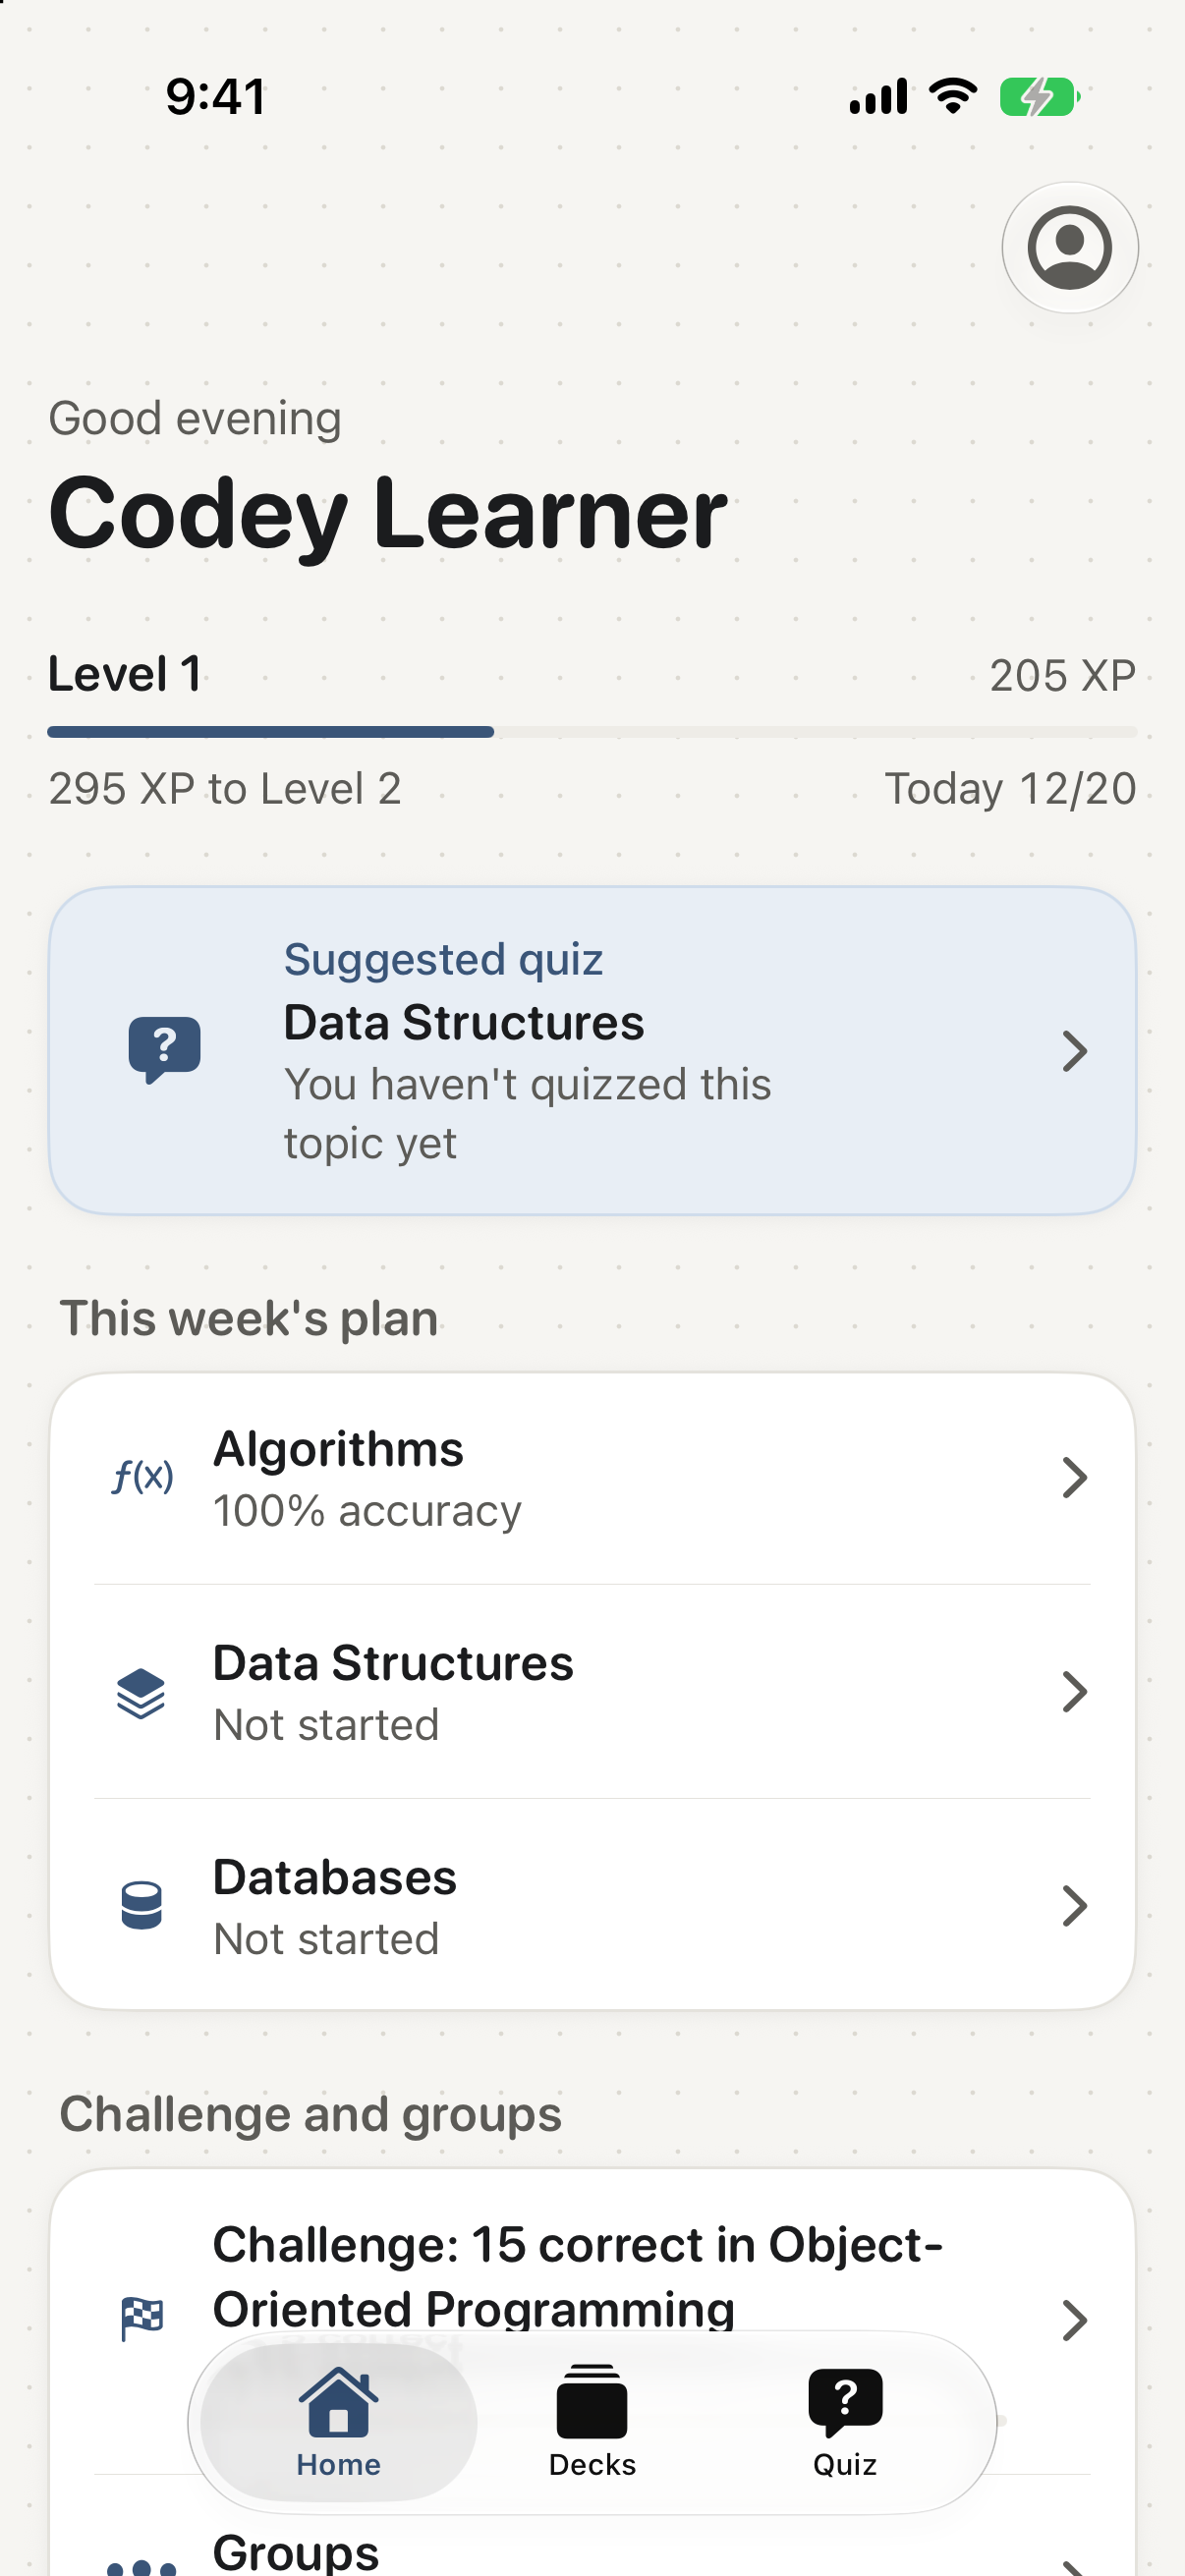
\includegraphics[width=0.235\textwidth]{home-light.png}\hfill
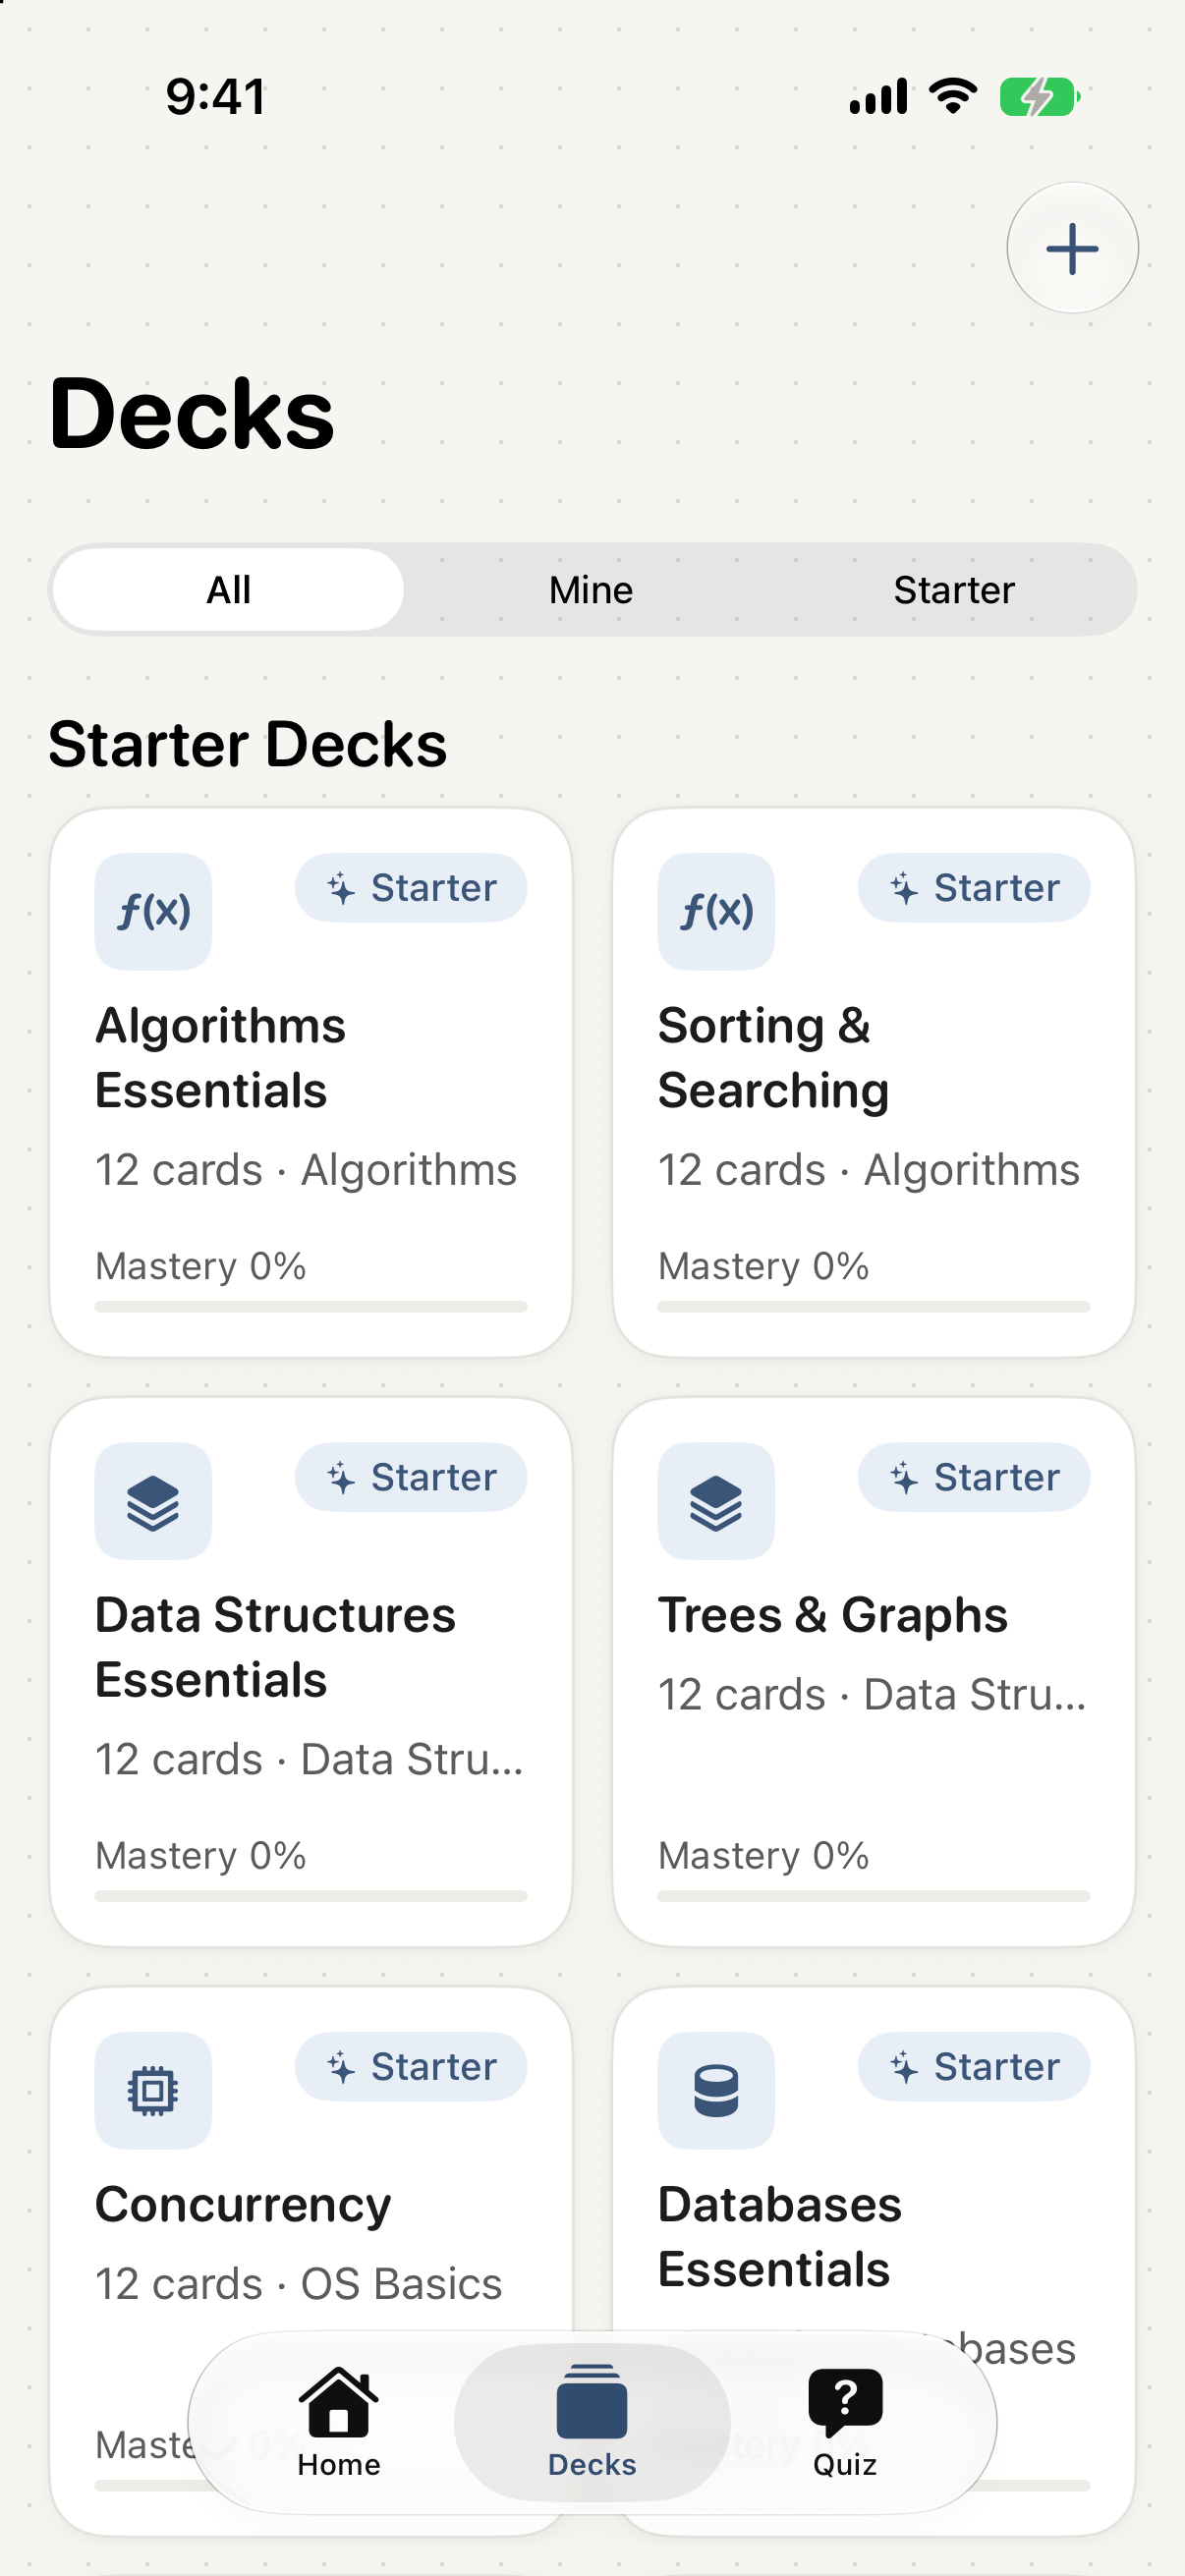
\includegraphics[width=0.235\textwidth]{decks.png}\hfill
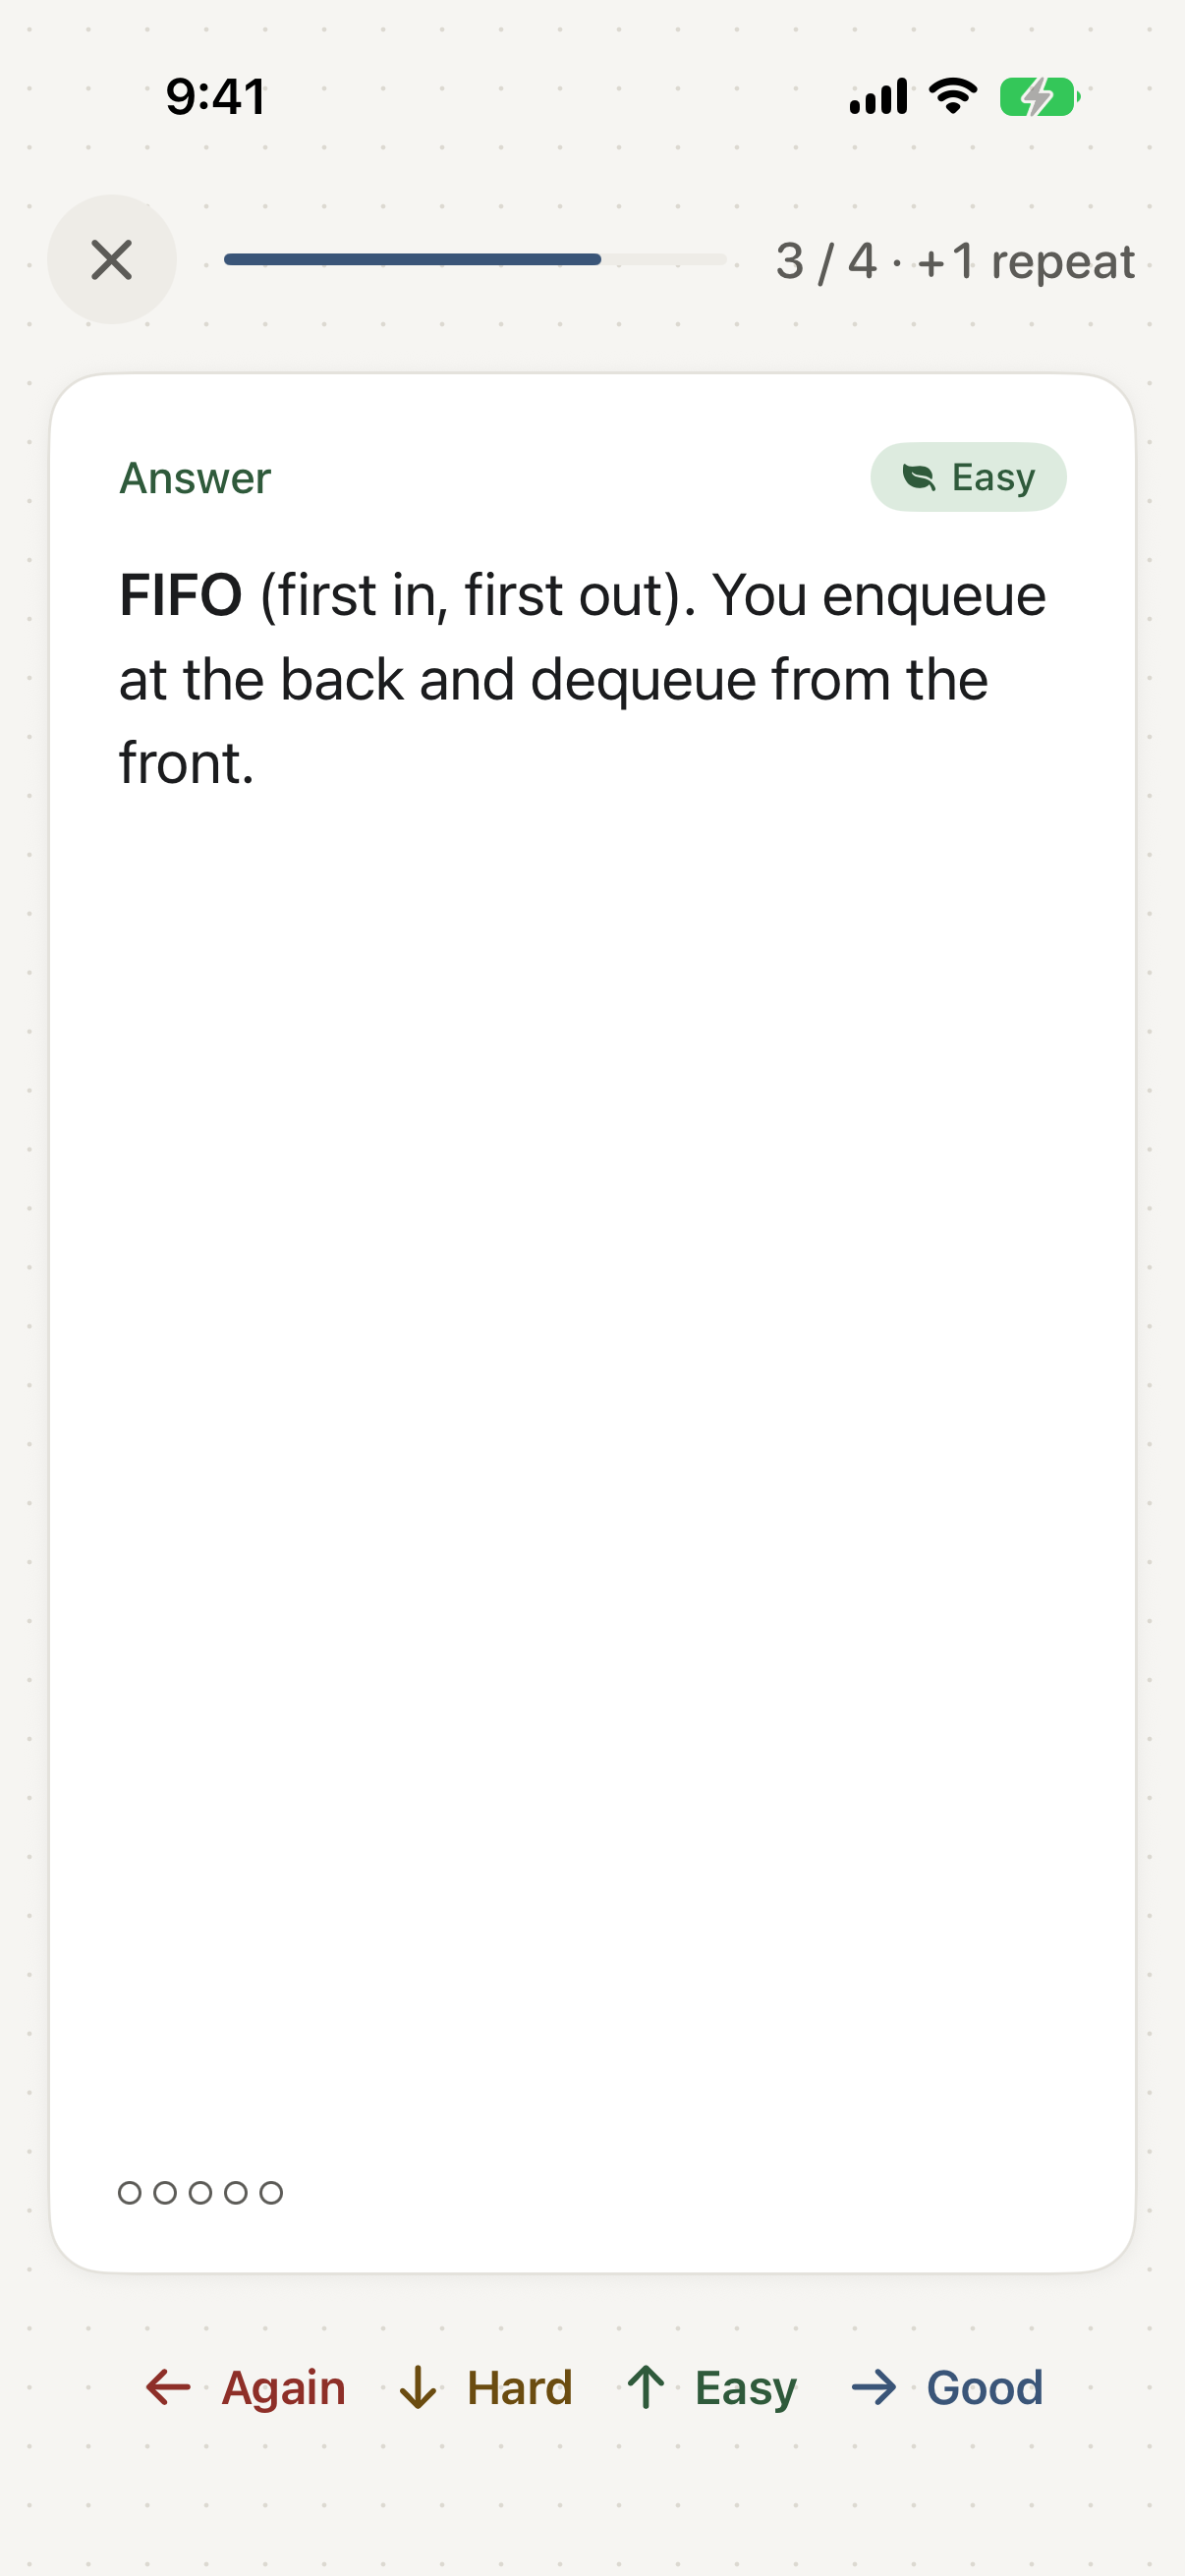
\includegraphics[width=0.235\textwidth]{study.png}\hfill
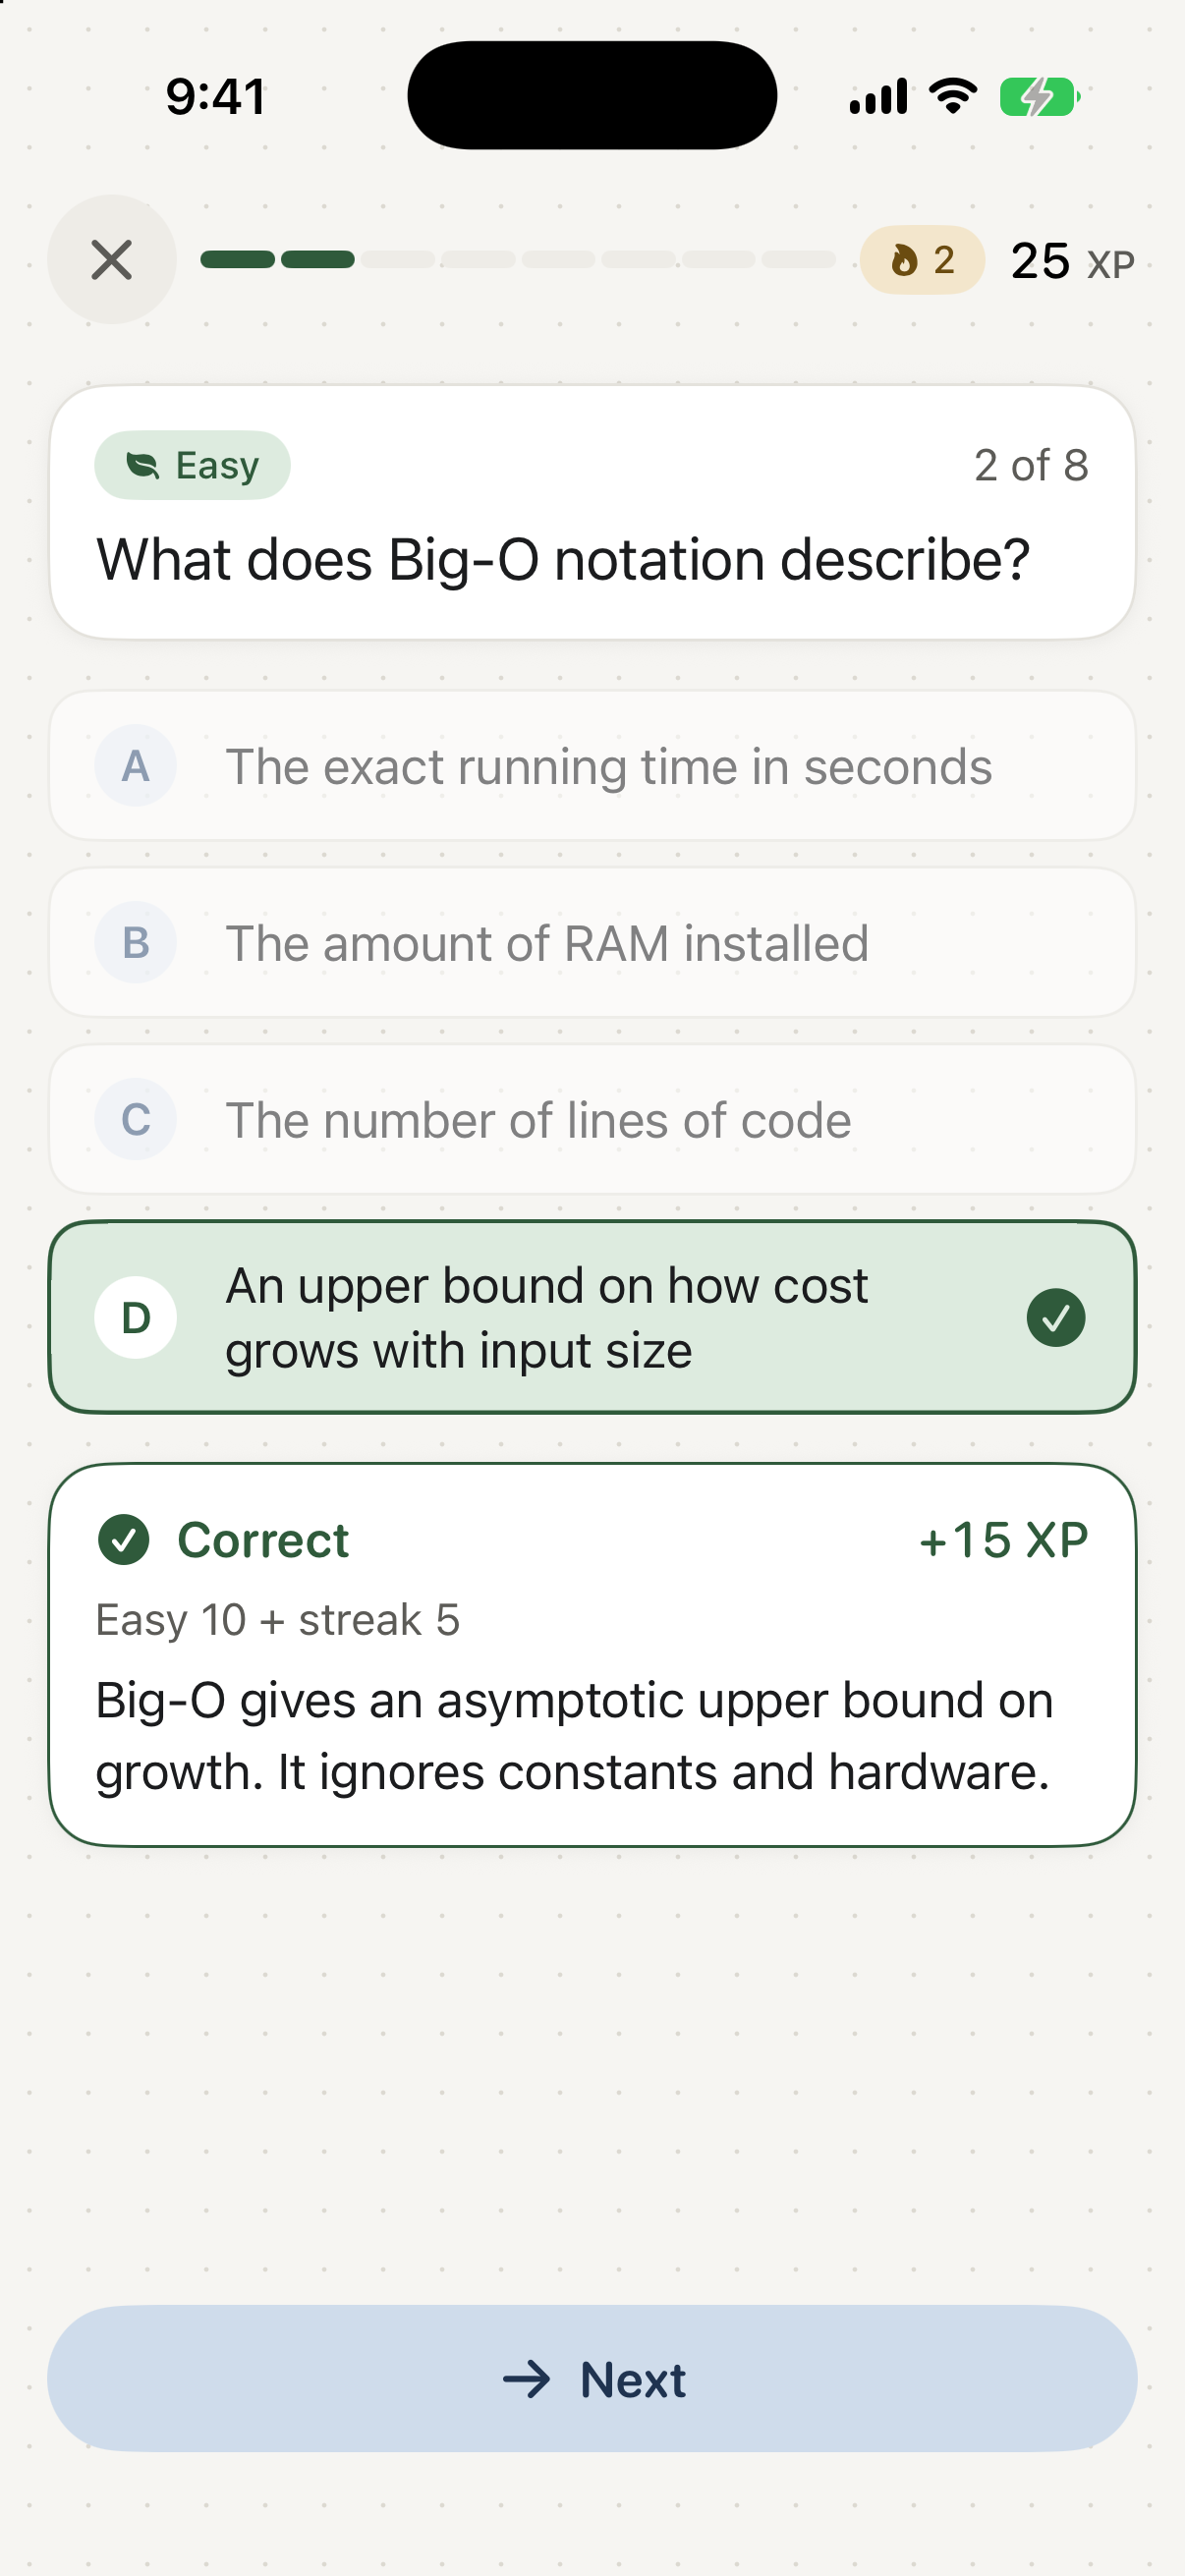
\includegraphics[width=0.235\textwidth]{quiz.png}\\[1ex]
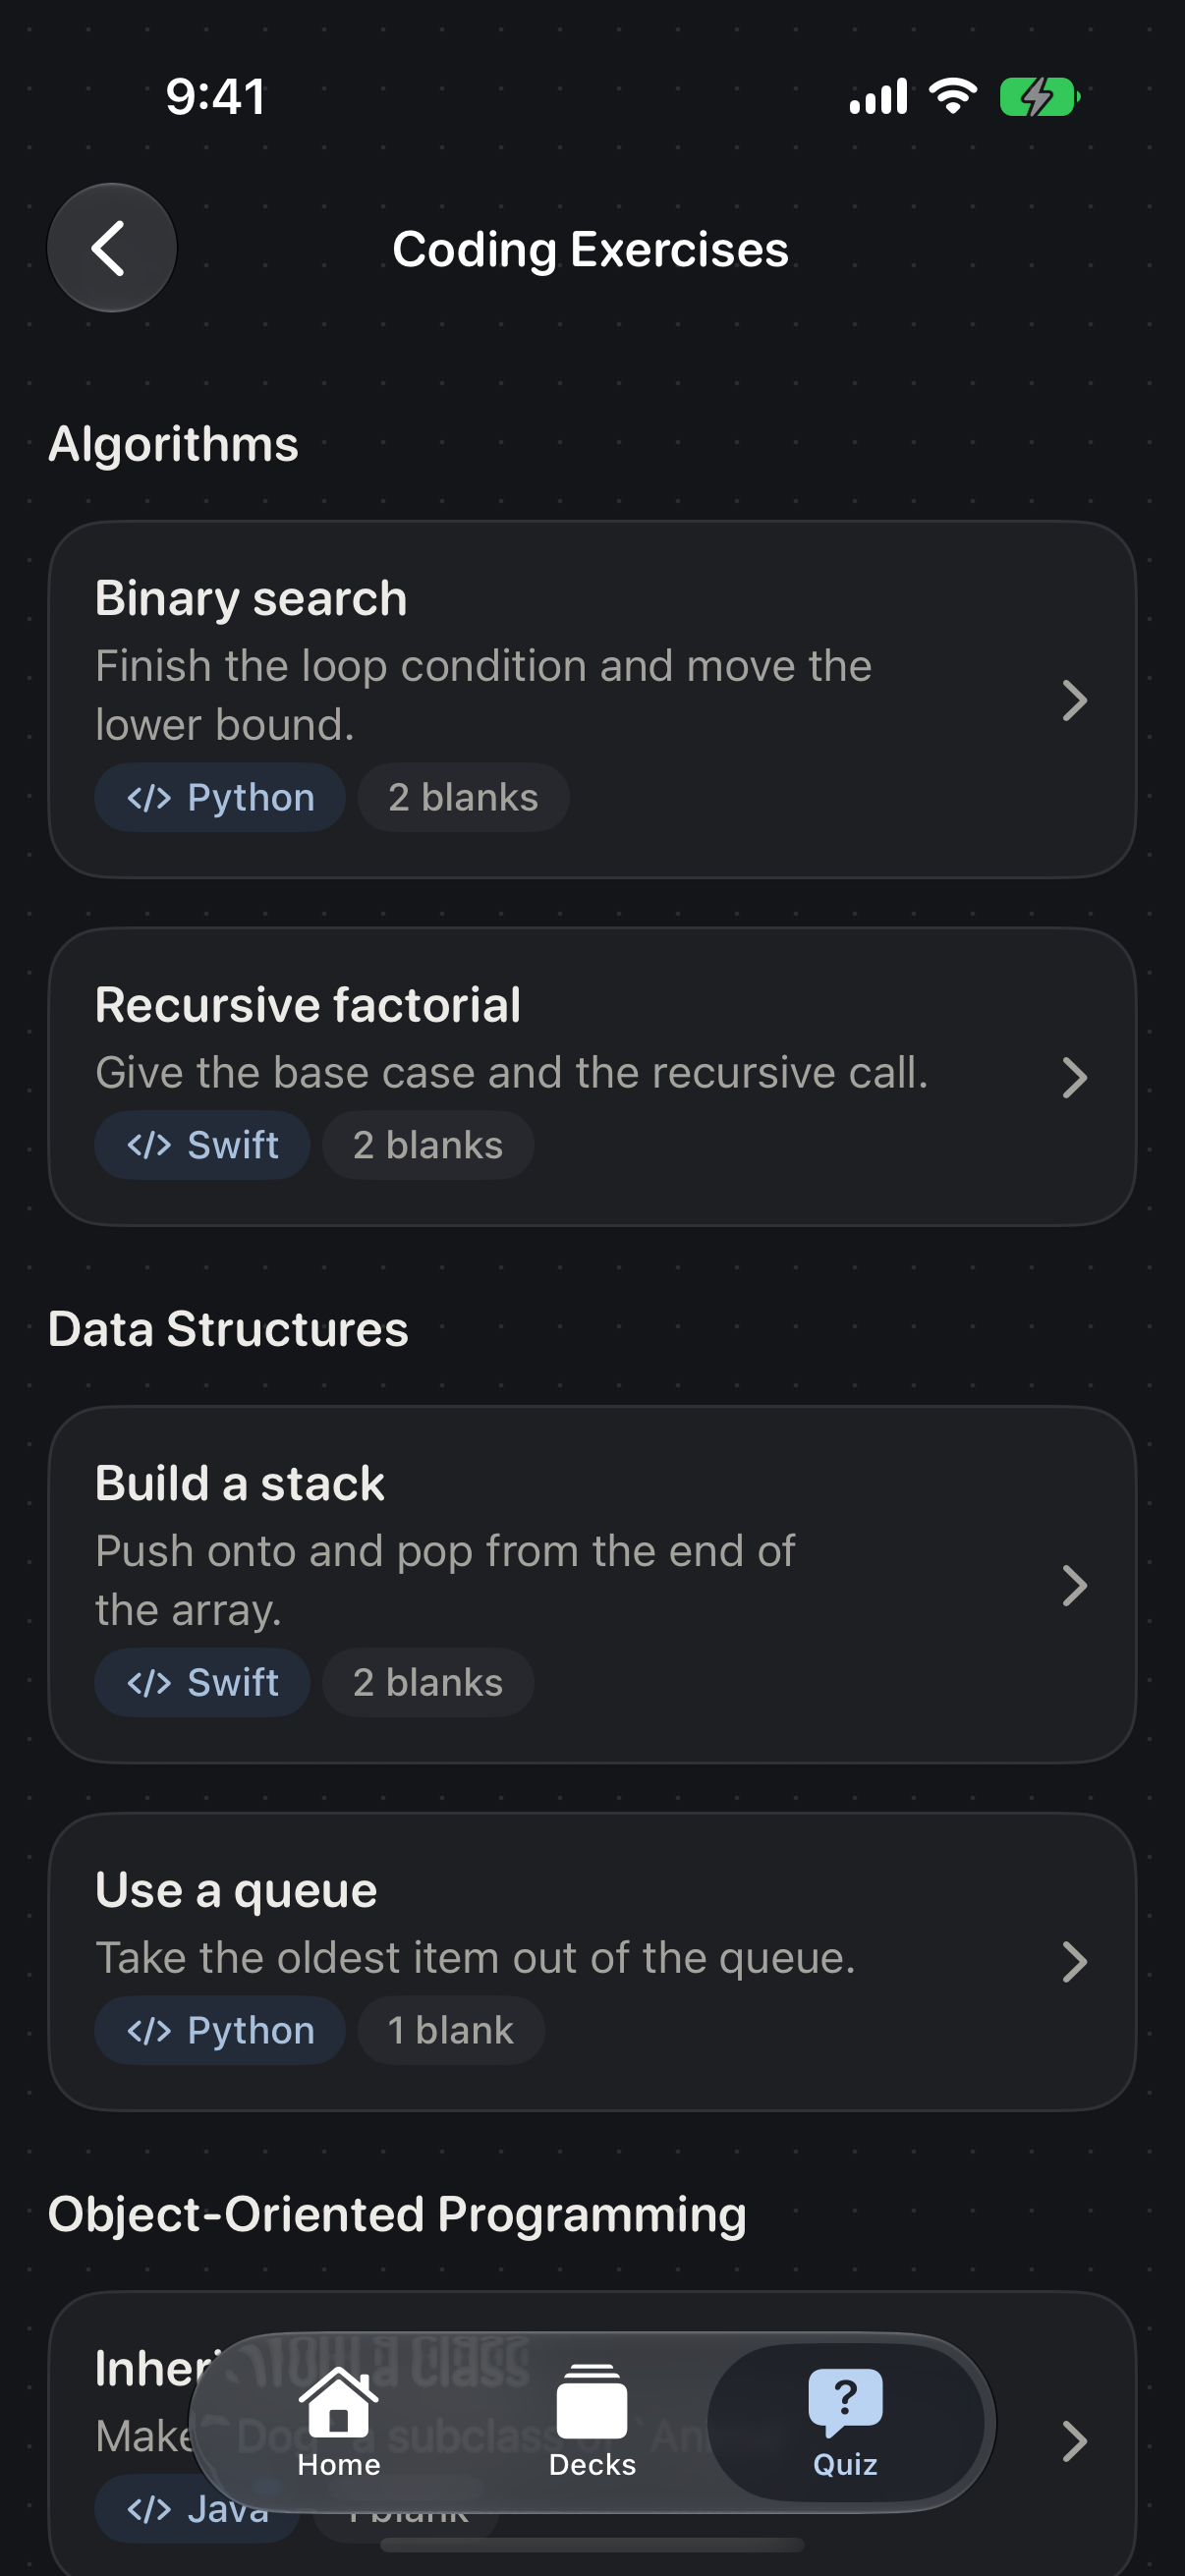
\includegraphics[width=0.235\textwidth]{exercise-list.png}\hfill
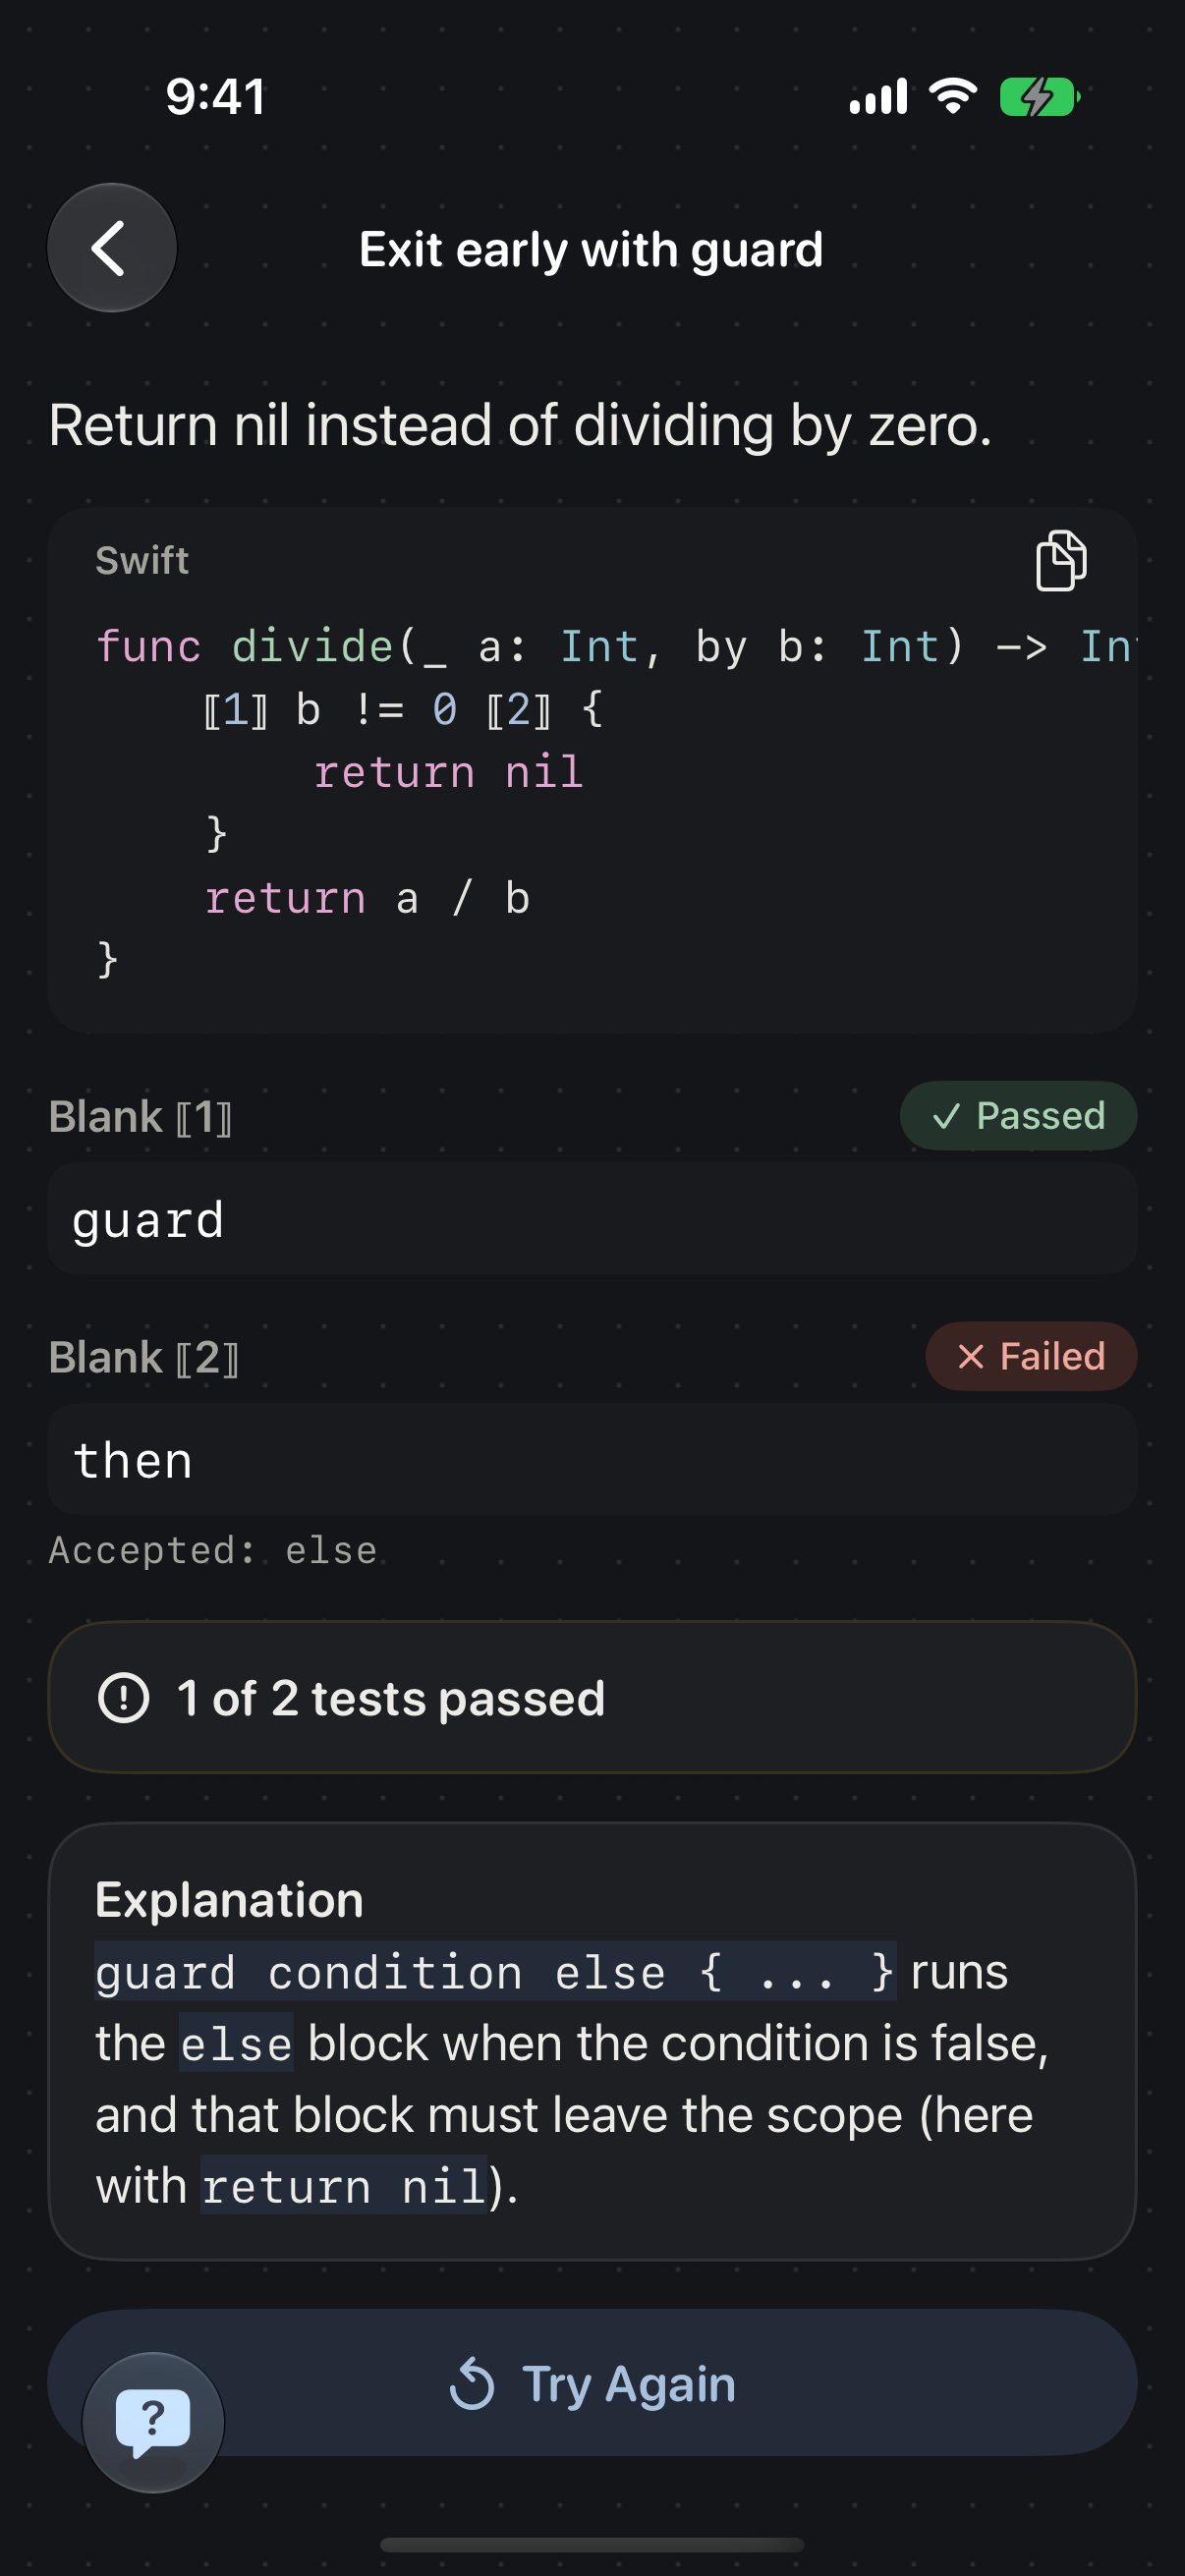
\includegraphics[width=0.235\textwidth]{exercise.png}\hfill
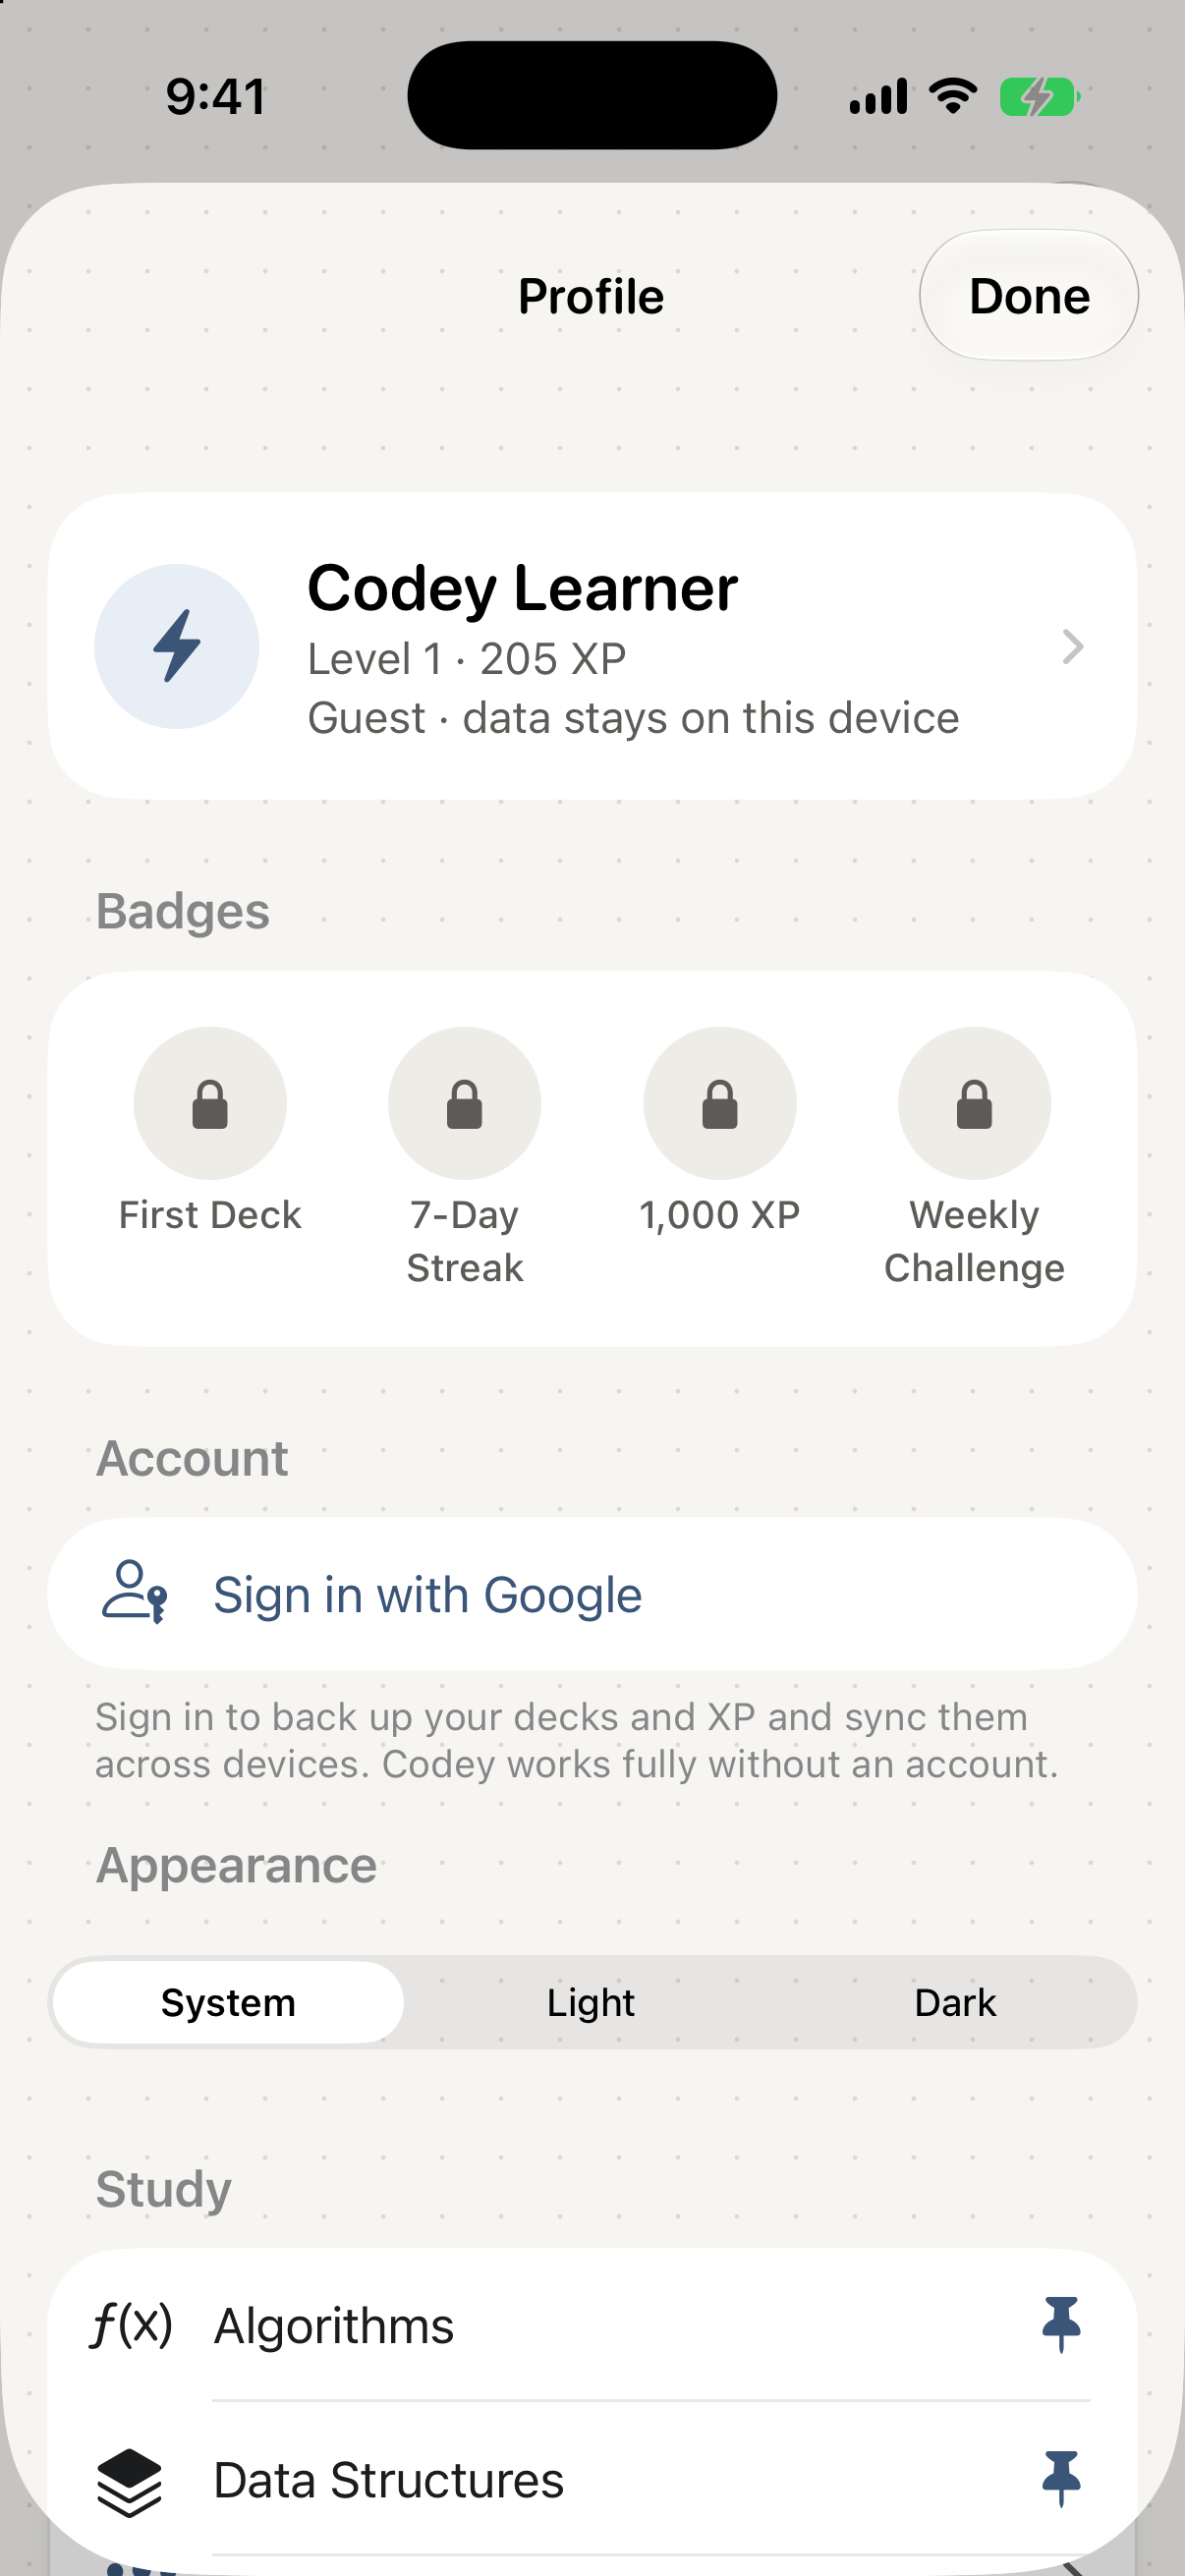
\includegraphics[width=0.235\textwidth]{profile.png}\hfill
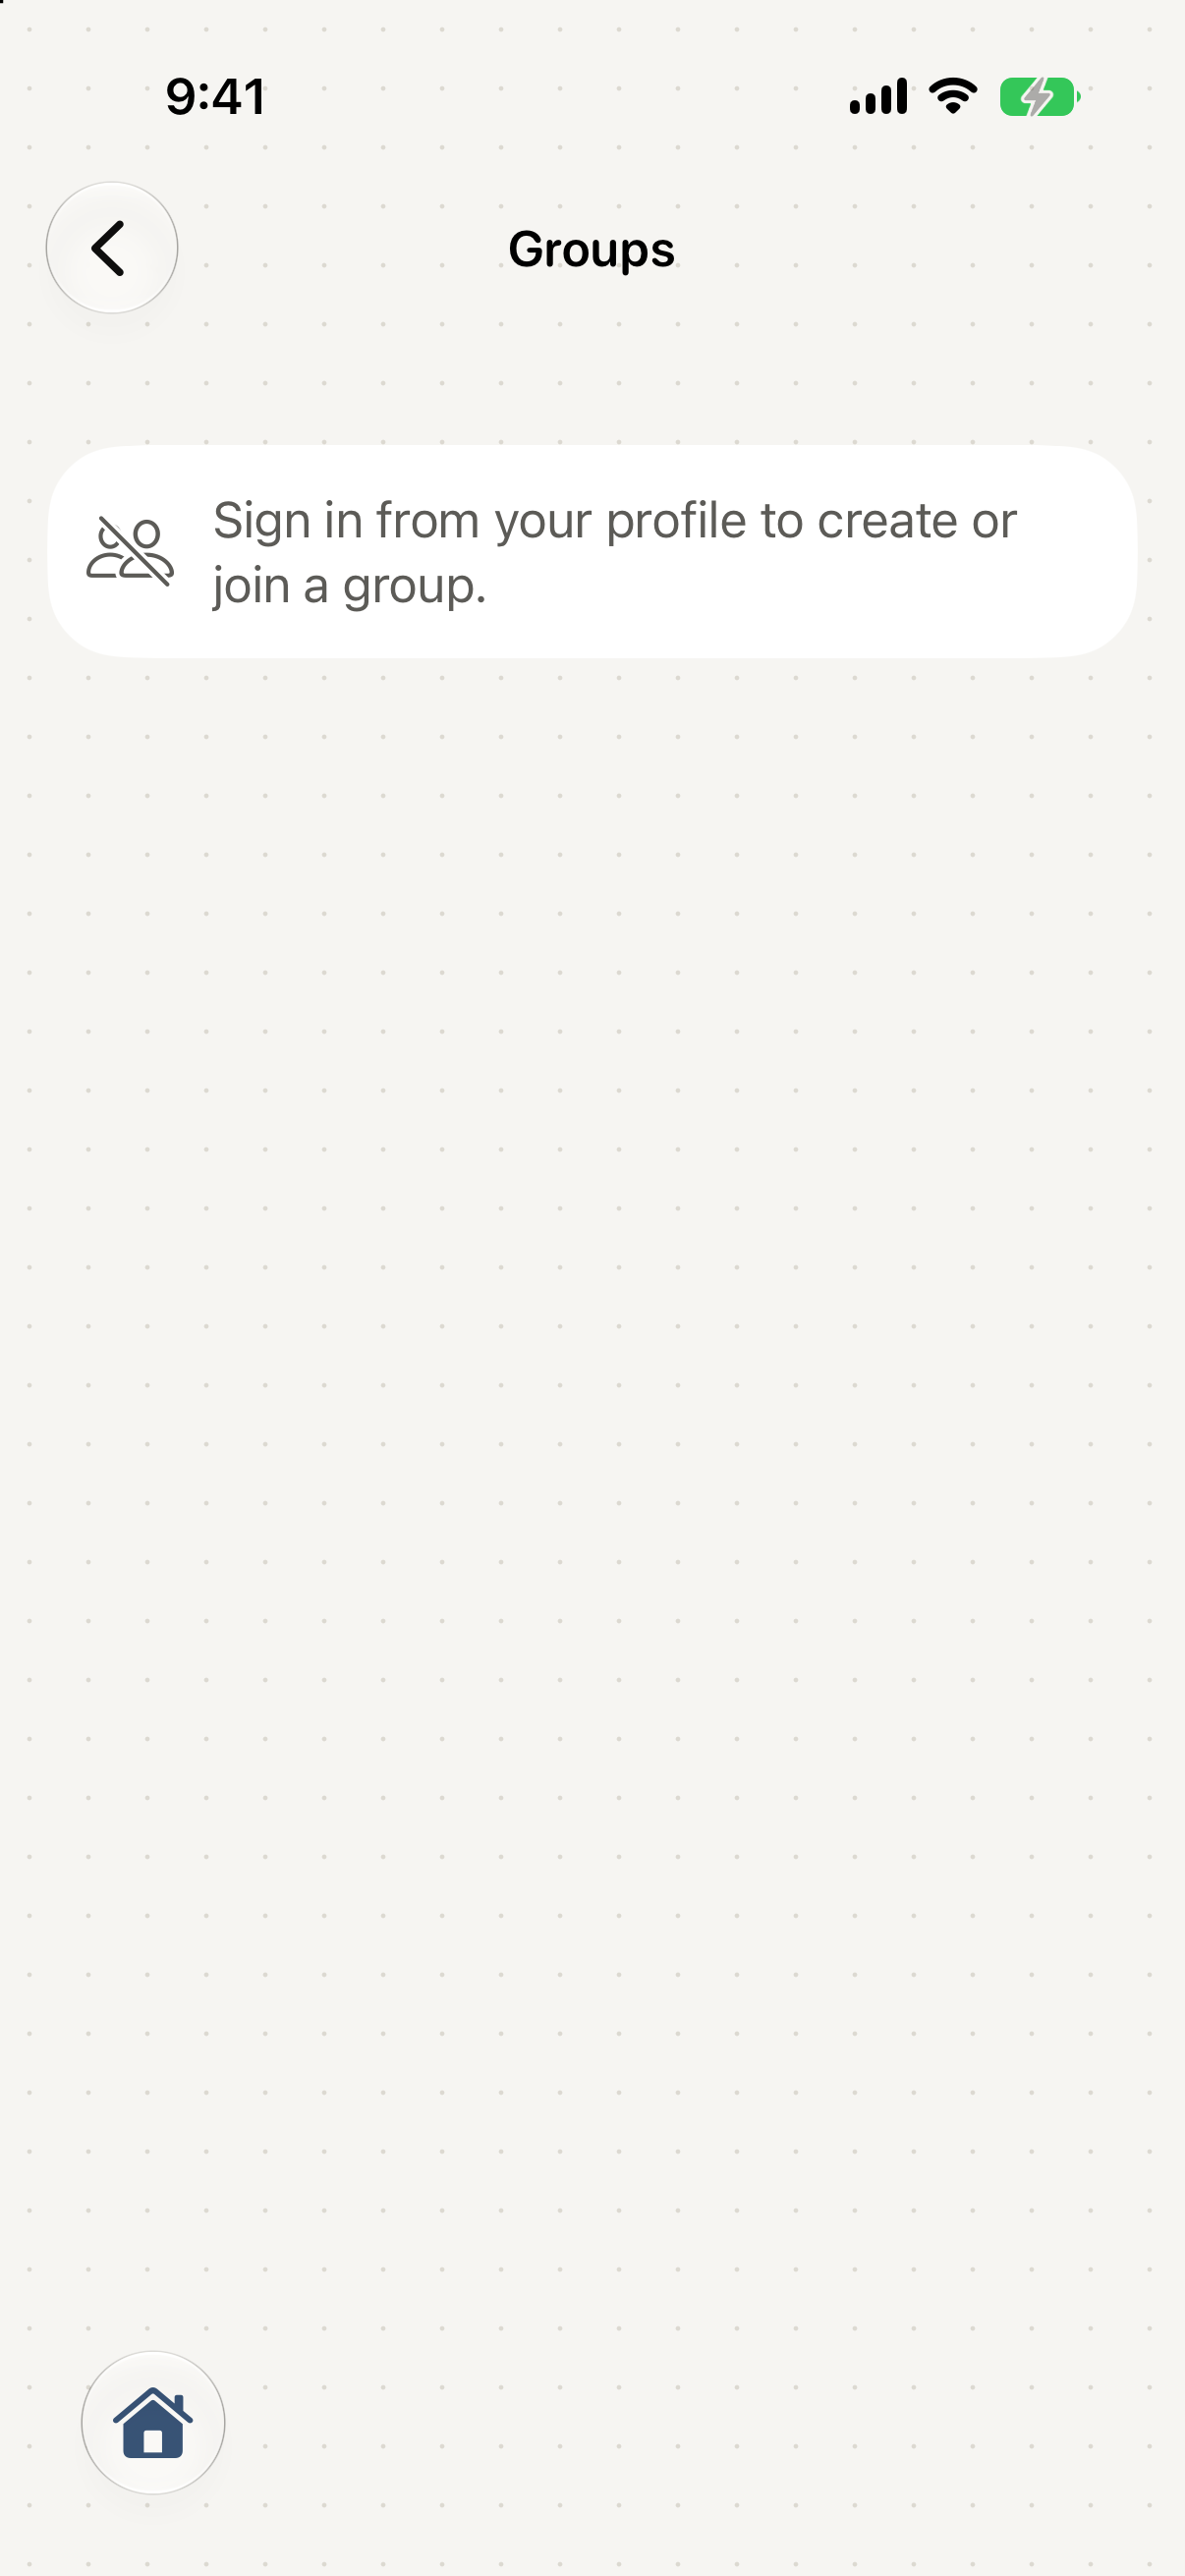
\includegraphics[width=0.235\textwidth]{groups.png}
\caption{Main screens (iOS Simulator). Top: Home, Decks, a study card (answer side), and a quiz question after a correct answer. Bottom: the coding-exercise list and an exercise after Check with one blank passed and one failed (Dark Mode, FR-39 to FR-41), the profile sheet, and Groups while signed out.}
\label{fig:screens}
\end{figure}

\subsection{Changes Since Sprint 3}
Sprint 4 was the testing sprint. It added no feature beyond the two client mandates
that were still open, and spent the rest of its time planning, running, and
documenting tests. The principal changes are:
\begin{itemize}
  \item \textbf{Coding exercises (FR-39 to FR-41).} Twelve code-completion exercises
        in Swift, Python, and Java across five topics. The student fills in each
        blank, and every blank is checked as one test case against its accepted
        answers after whitespace normalization. No code is compiled or executed on
        the device (decision S31).
  \item \textbf{Study-results sync (FR-61).} Card mastery, quiz-question progress,
        and tier unlocks now sync per account through three new Supabase tables with
        Row Level Security and merge triggers (decision S32).
  \item \textbf{Two defects fixed.} Google Sign-In crashed on tap (BUG-01), and a
        successful Google sign-in did not sign the student in to Codey (BUG-02).
        Both have regression tests (Section~\ref{sec:defects}).
  \item \textbf{Testing.} A test plan, unit-test results with coverage, flow-graph
        test design, integration, system, and acceptance tests
        (Section~\ref{sec:testing}). Continuous integration now runs on both
        \texttt{main} and \texttt{dev} in three jobs: repository checks, the 75
        database tests, and the app tests with a per-test report and coverage.
  \item \textbf{Cuts.} The live-network leaderboard requirement (NFR-32), the live
        test accounts, and the peer usability study were dropped because they could
        not be verified within the sprint; R13 (client-reported weekly XP) was
        accepted with its rate limit (decisions S33, S34).
  \item \textbf{Fixes from November 2--5.} Swift 6 language mode, the first CI
        workflow, a server-side weekly-XP pace limit, and two launch-time fixes
        (no minimum loading screen, bundled content seeded only once).
  \item \textbf{Documentation.} New sections cover software testing
        (Section~\ref{sec:testing}) and concluding remarks
        (Section~\ref{sec:conclusion}). The UI design section and the change lists
        of earlier sprints were removed (they are in the Sprint 2 and 3 documents).
\end{itemize}

\subsection{Scope}
Table~\ref{tab:scope} defines the project scope. Every feature on the client's
mandatory list is built: XP, streaks, badges, analytics, the personalized study
plan, leaderboards and weekly challenges, offline use with cloud sync of decks and
study results (FR-61), and the coding challenges (FR-39 to FR-41). Table~\ref{tab:moscow}
prioritizes features using the MoSCoW method. Could Have features were built last,
and open-ended coding problems were dropped as planned under risk R1.

The client-mandated coding challenges are scoped as code-completion
(fill-in-the-blank) exercises. Each answer is validated by comparison with accepted
solutions, so no code is compiled or executed on the device. Open-ended,
LeetCode-style problems that require running arbitrary code are a stretch goal. No
code-execution prototype was built, so, as planned under risk R1, open-ended
problems were dropped and are listed as future work (Section~\ref{sec:conclusion}).

\begin{table}[H]
\centering
\caption{In-scope and out-of-scope features (updated for Sprint 4)}
\label{tab:scope}
\begin{tabularx}{\textwidth}{@{}Y Y@{}}
\toprule
\textbf{In Scope (will build)} & \textbf{Out of Scope (will not build)} \\
\midrule
User-built flashcard decks with optional code snippets, plus bundled starter decks & Multi-language (localization) support \\
Adaptive practice with Easy/Medium/Hard question tiers that rotate as questions are mastered & Real-time multiplayer (leaderboards and weekly challenges are asynchronous) \\
XP, levels, streaks, and badges & Advertisements and in-app purchases \\
Per-topic progress analytics and personalized study plans & Direct messaging between users \\
Code-completion (fill-in-the-blank) exercises with automated validation & Full IDE functionality \\
Leaderboards and weekly challenges (class, club, or friends list) & Importing decks from files (user decks are built in the app; starter decks are bundled) \\
Offline data caching and cloud sync & App Store distribution (demonstrated from Xcode only) \\
Secure data handling (encryption and row-level access control) & Paid third-party services \\
\bottomrule
\end{tabularx}
\end{table}

\begin{table}[H]
\centering
\caption{Feature prioritization (MoSCoW)}
\label{tab:moscow}
\begin{tabularx}{\textwidth}{@{}Y Y Y@{}}
\toprule
\textbf{Must Have} & \textbf{Should Have} & \textbf{Could Have} \\
\midrule
User-created flashcards & Code snippets on cards & Customized profile \\
Working SwiftUI interface & Levels & Defect reports \\
Easy/Medium/Hard difficulty & Dark/Light mode & Open-ended coding problems (dropped, R1) \\
Adaptive tier rotation (client mandate) & Starter decks & \\
XP, daily streaks, and badges (client mandate) & Review returns of retired questions & \\
Progress analytics and personalized study plan (client mandate) & Guest-mode upload, sync retries, conflict merge, and sync status & \\
Offline use with cloud sync of decks (client mandate) & & \\
Navigation that adapts to all supported iPhone screen sizes (NFR-10) & & \\
Stable operation (no crashes during scripted test sessions) & & \\
Code-completion exercises (client mandate) & & \\
Leaderboards and weekly challenges (client mandate) & & \\
Offline sync of study results (client mandate) & & \\
\bottomrule
\end{tabularx}
\end{table}

% =====================================================================
\section{Requirements (Updated for Sprint 4)}\label{sec:reqs}
% =====================================================================
Requirements are written in accordance with ISO/IEC/IEEE 29148:2018. Each
requirement is a single, verifiable ``shall'' statement with a unique identifier that
is referenced in the traceability matrices (Section~\ref{sec:trace}). \emph{Priority}
follows the MoSCoW scale in Table~\ref{tab:moscow}. \emph{Source} indicates whether
the requirement originates from the client's mandatory list or from the team.
\emph{Status} reflects progress at the time of submission: \emph{Implemented} (built,
covered by passing tests, and merged) or \emph{Retired} (dropped, with the reason
given). Sprint 4 closes every requirement: no requirement is planned or in progress. Sprint 1 requirements that specified
more than one behavior were decomposed in Sprint 2, and identifiers were reassigned
accordingly. In Sprint 3 the remaining compound requirements were split so that each
has one testable behavior. To keep every identifier stable, the original requirement
keeps its number and the split-off behavior receives a new number: FR-03 $\to$ FR-54,
FR-12 $\to$ FR-55, FR-24 $\to$ FR-56 and FR-57, FR-28 $\to$ FR-58, FR-47 $\to$ FR-59,
FR-04 $\to$ FR-60, FR-08 $\to$ FR-62, FR-14 $\to$ FR-63, FR-15 $\to$ FR-64,
FR-45 $\to$ FR-65, and FR-46 $\to$ FR-66. The compound leaderboard requirement FR-42
was split into FR-42 and FR-50 to FR-53, and FR-61 was added for the client's offline
results mandate. Every requirement whose source is the client's mandatory list has
Must priority. In Sprint 4, FR-39 to FR-41 and FR-61 moved from Planned to
Implemented, and NFR-32 was retired (decision S33). The functional requirements
number 66, all implemented, and the non-functional requirements 32, of which 31 are
in force.

\subsection{Functional Requirements}

\begin{xltabular}{\textwidth}{@{}l Y l l l@{}}
\caption{Functional requirements}\label{tab:fr}\\
\toprule
\textbf{ID} & \textbf{Requirement} & \textbf{Priority} & \textbf{Source} & \textbf{Status} \\
\midrule
\endfirsthead
\multicolumn{5}{@{}l}{\small\itshape Table \thetable\ continued} \\
\toprule
\textbf{ID} & \textbf{Requirement} & \textbf{Priority} & \textbf{Source} & \textbf{Status} \\
\midrule
\endhead
\bottomrule
\endfoot
\multicolumn{5}{@{}l}{\textit{Account and authentication}} \\
FR-01 & The app shall allow a user to sign in with a Google account through Supabase Auth. & Must & Team & Implemented \\
FR-02 & The app shall store the authenticated session token in the iOS Keychain. & Must & Client & Implemented \\
FR-03 & The app shall allow a signed-in user to sign out, which deletes the stored session token from the Keychain. & Must & Team & Implemented \\
FR-54 & When signing out, the app shall let the user choose whether to keep or remove that account's decks on the device. & Must & Team & Implemented \\
FR-04 & The app shall allow a user to set a display name of 1--30 characters (trimmed, counted in Unicode scalars). & Could & Team & Implemented \\
FR-60 & The app shall allow a user to choose an avatar from a predefined set of 12 symbols, synchronized to the user's profile. & Could & Team & Implemented \\
\multicolumn{5}{@{}l}{\textit{Decks and flashcards}} \\
FR-05 & The app shall allow a user to create a flashcard deck with a title of 1--60 characters and a topic category chosen from a predefined list. & Must & Team & Implemented \\
FR-06 & The app shall allow a user to add a flashcard with a prompt and an answer of 1--500 characters each to a deck. & Must & Team & Implemented \\
FR-07 & The app shall allow a user to attach an optional code snippet (language and source text) to a flashcard. & Should & Team & Implemented \\
FR-08 & The app shall render card prompts and answers as Markdown. & Should & Team & Implemented \\
FR-62 & The app shall display code snippets with syntax highlighting for Swift, Python, Java, and C++. & Should & Team & Implemented \\
FR-09 & The app shall validate every flashcard against the JSON card schema (\texttt{flashcard.schema.json}, encoded as \texttt{FlashcardPayload}) before saving it. & Must & Team & Implemented \\
FR-10 & The app shall show an inline error message next to each field that fails validation. & Must & Team & Implemented \\
FR-11 & The app shall allow a user to edit the prompt, answer, or code snippet of an existing flashcard. & Must & Team & Implemented \\
FR-12 & The app shall allow a user to delete a deck after confirming a deletion prompt. & Must & Team & Implemented \\
FR-55 & The app shall propagate a deleted deck that was synced before to Supabase on the next sync. & Must & Team & Implemented \\
FR-13 & The app shall allow a user to delete an individual flashcard from a deck. & Must & Team & Implemented \\
FR-14 & The app shall include at least one developer-authored starter deck for each predefined topic category, bundled with the app (\texttt{starter-decks.json}). & Should & Team & Implemented \\
FR-63 & The app shall tag every starter-deck card with exactly one difficulty tier: Easy, Medium, or Hard. & Should & Team & Implemented \\
FR-15 & The app shall allow a user to toggle a starter deck between hidden and shown in the deck library. & Should & Team & Implemented \\
FR-64 & The app shall prevent a user from editing or deleting a starter deck. & Should & Team & Implemented \\
\multicolumn{5}{@{}l}{\textit{Study and quizzes}} \\
FR-16 & The app shall present the cards of a selected deck one at a time, with the answer hidden until the user taps the card. & Must & Team & Implemented \\
FR-17 & The app shall let the user rate a revealed card as Again, Hard, Good, or Easy. & Must & Team & Implemented \\
FR-18 & The app shall update a card's mastery score after each rating given in FR-17: Again resets the score to 0, Hard leaves it unchanged, Good adds 1, and Easy adds 2, up to a maximum of 5. A card with a score of 5 is considered mastered. & Must & Team & Implemented \\
FR-19 & The app shall generate a multiple-choice quiz of up to 10 questions from the question bank for a user-selected topic (fewer when the active pool is smaller). & Must & Client & Implemented \\
FR-20 & The app shall display the score (correct/total and percentage) at the end of each quiz. & Must & Team & Implemented \\
FR-21 & The app shall organize the question bank by computer science topic: Data Structures, Algorithms, OS Basics, Databases, Object-Oriented Programming, Networking, Swift Basics, and Python Basics. & Must & Team & Implemented \\
\multicolumn{5}{@{}l}{\textit{Adaptive practice}} \\
FR-22 & The app shall tag each question in the question bank with exactly one difficulty tier: Easy, Medium, or Hard. & Must & Client & Implemented \\
FR-23 & The app shall record, for each user and question, the number of consecutive correct answers; an incorrect answer resets this count to zero. & Must & Client & Implemented \\
FR-24 & The app shall retire a question from the user's active practice pool after it has been answered correctly 3 consecutive times. & Must & Client & Implemented \\
FR-56 & The app shall retire a starter-deck card from study when its mastery score reaches 5. & Must & Client & Implemented \\
FR-57 & The app shall keep a tier unlocked for a topic once it has been unlocked, even if review returns lower the retired count. & Must & Client & Implemented \\
FR-25 & The app shall add a topic's Medium questions to the user's active pool when at least 70\% of that topic's Easy questions are retired. & Must & Client & Implemented \\
FR-26 & The app shall add a topic's Hard questions to the user's active pool when at least 70\% of that topic's Medium questions are retired and the user is level 3 or higher. & Must & Client & Implemented \\
FR-27 & The app shall draw at least 70\% of each quiz's questions from the highest unlocked tier for that topic and the rest from lower unlocked tiers. If only the Easy tier is unlocked, all questions shall be drawn from it. & Must & Client & Implemented \\
FR-28 & The app shall return a retired question to the user's active pool as a review question 7 days after it was retired. & Should & Team & Implemented \\
FR-58 & The app shall retire a review question again after one correct answer, and reset its consecutive correct count to zero after an incorrect answer. & Should & Team & Implemented \\
FR-29 & The app shall let the user restrict a practice session to any single tier they have unlocked for the selected topic. & Must & Team & Implemented \\
\multicolumn{5}{@{}l}{\textit{Gamification}} \\
FR-30 & The app shall award XP for each correctly answered quiz question equal to a tier base (Easy 10, Medium 15, Hard 20) plus a streak bonus of $\min(5\times(\text{streak}-1), 25)$, for at most 45 XP per answer. & Must & Client & Implemented \\
FR-31 & The app shall compute the user's level as $\lfloor \text{XP}/500 \rfloor + 1$. & Should & Team & Implemented \\
FR-32 & The app shall mark the daily goal as met when the user answers 20 questions (quiz questions answered plus flashcards rated) within one calendar day in the device's time zone. & Must & Client & Implemented \\
FR-33 & The app shall set the daily streak to 1 on a day the daily goal is met following a day it was not met, and increase it by one for each subsequent consecutive day the goal is met. & Must & Client & Implemented \\
FR-34 & The app shall reset the daily streak to zero after a calendar day in which the daily goal was not met. & Must & Client & Implemented \\
FR-35 & The app shall award a badge for each of four milestones: saving a first deck, reaching a 7-day streak, earning 1,000 total XP, and completing a weekly challenge; an earned badge stays earned. & Must & Client & Implemented \\
\multicolumn{5}{@{}l}{\textit{Progress and analytics}} \\
FR-36 & The app shall calculate per-topic accuracy as the percentage of correct answers over the user's last 50 quiz answers in that topic. & Must & Client & Implemented \\
FR-37 & The app shall display a home dashboard showing total XP, level, current streak, and per-topic accuracy. & Must & Client & Implemented \\
FR-38 & The app shall generate a weekly study plan that recommends the three topics with the lowest accuracy (topics with fewer than 5 answers first), fixed until the next Monday. & Must & Client & Implemented \\
\multicolumn{5}{@{}l}{\textit{Code-completion exercises}} \\
FR-39 & The app shall provide code-completion exercises in which the user types the missing token or expression for each blank of a code snippet. & Must & Client & Implemented \\
FR-40 & The app shall validate each completed blank against the exercise's automated test cases, which compare the answer with the accepted solutions after whitespace normalization. & Must & Client & Implemented \\
FR-41 & The app shall show a pass or fail result for each test case after a submission is validated. & Must & Client & Implemented \\
\multicolumn{5}{@{}l}{\textit{Social competition}} \\
FR-42 & The app shall display a weekly leaderboard that ranks the members of a group the user belongs to by XP earned since the most recent Monday at 00:00 UTC. & Must & Client & Implemented \\
FR-43 & The app shall publish one weekly challenge (15 correct quiz answers in a topic chosen by ISO week number) that resets every Monday at 00:00 UTC. & Must & Client & Implemented \\
FR-50 & The app shall allow a signed-in user to create a group with a name of 1--40 characters, and shall show the group's six-character invite code generated by the server. & Must & Client & Implemented \\
FR-51 & The app shall allow a signed-in user to join a group by entering a valid six-character invite code (case-insensitive). & Must & Client & Implemented \\
FR-52 & The app shall allow a user to leave a group. & Must & Team & Implemented \\
FR-53 & The app shall show the user's weekly challenge progress (correct answers out of 15) on the home dashboard. & Must & Team & Implemented \\
\multicolumn{5}{@{}l}{\textit{Offline operation and synchronization}} \\
FR-44 & The app shall save every new or edited deck to the local SwiftData store before making any network request. & Must & Client & Implemented \\
FR-45 & The app shall queue every local change to decks, cards, and the profile's XP for synchronization, including changes made while offline or signed out. & Must & Client & Implemented \\
FR-65 & The app shall upload the changes queued while the user was signed out after the user's first sign-in. & Should & Team & Implemented \\
FR-46 & The app shall push queued changes to Supabase and pull remote changes automatically when connectivity is restored. & Must & Client & Implemented \\
FR-66 & The app shall retry a failed synchronization with exponential backoff, from 2 seconds up to 300 seconds. & Should & Team & Implemented \\
FR-47 & The app shall resolve a sync conflict with an additive merge that keeps every card present in either the local or the remote version. & Should & Team & Implemented \\
FR-59 & When the same card has been edited in both versions of a conflicting deck, the app shall keep the version with the later modification timestamp. & Should & Team & Implemented \\
FR-48 & The app shall show each deck's sync status (Draft, Saved locally, Syncing, Synced, or Conflict) in the deck library. & Should & Team & Implemented \\
FR-61 & The app shall sync a signed-in user's study results (card mastery scores, quiz question progress, and tier unlocks) to Supabase when connectivity is restored, keeping the most recent review when two devices differ. & Must & Client & Implemented \\
\multicolumn{5}{@{}l}{\textit{Feedback}} \\
FR-49 & The app shall allow a signed-in user to submit a UI/UX defect report with a text description of 1--1,000 characters, which is stored in Supabase for review by the development team. & Could & Team & Implemented \\
\end{xltabular}

\subsection{Adaptive Practice Rationale}
The client requires practice that adjusts difficulty to recent performance. FR-22 to
FR-29 implement this as a tiered pool: a question answered correctly three times in a
row retires, the next tier opens when 70\% of the current one has retired, quizzes
draw mostly from the highest open tier, and retired questions return for review after
seven days. The thresholds live in one type, \texttt{GatingConfig}, so they can be
tuned without code changes elsewhere, and tier unlocks are permanent. Starter-deck
cards follow the same gating (a card retires at mastery 5), and every topic has at
least 8 Easy, 8 Medium, and 6 Hard questions so the 70/30 mix works from the first
quiz.

\subsection{Non-Functional Requirements}

\begin{xltabular}{\textwidth}{@{}l L{2.1cm} Y L{4.3cm}@{}}
\caption{Non-functional requirements}\label{tab:nfr}\\
\toprule
\textbf{ID} & \textbf{Category} & \textbf{Requirement} & \textbf{Verification Method} \\
\midrule
\endfirsthead
\multicolumn{4}{@{}l}{\small\itshape Table \thetable\ continued} \\
\toprule
\textbf{ID} & \textbf{Category} & \textbf{Requirement} & \textbf{Verification Method} \\
\midrule
\endhead
\bottomrule
\endfoot
NFR-01 & Performance & The home dashboard shall finish loading within 3 seconds of app launch on a standard mobile data connection (95th percentile). & TC-P08: \texttt{LaunchTimer} logs process start to Home's first appearance; \texttt{scripts/perf-launch.sh} relaunches the app 10 times on the Simulator. Launch makes no network request, so the network profile does not change the result. \\
NFR-02 & Performance & A 100-card deck shall finish syncing to Supabase within 5 seconds on Wi-Fi, measured from the start of the push to receipt of the server's acknowledgment. & TC-P07 against a mock backend with 50 ms per request. Not measured live: the live test accounts were dropped (S33). \\
NFR-03 & Compatibility & The app shall build and run on the latest public iOS release, with a minimum deployment target of iOS 26. & Build and smoke test on the latest iOS Simulator runtime (iOS 27). \\
NFR-04 & Security & The local SwiftData store shall be encrypted at rest using iOS Data Protection (\emph{complete unless open} file protection, so a sync in progress can finish after the device locks). & \texttt{StoreFileProtectionTests} sets and checks the protection class; the attribute itself is read on a physical device (TC-S10), because the Simulator does not store it. \\
NFR-05 & Security & All user data stored in the cloud database shall be encrypted at rest (AES-256). & Review Supabase project security settings and the provider's encryption-at-rest documentation. \\
NFR-06 & Security & All client--server traffic shall use HTTPS with TLS 1.3, with no App Transport Security exceptions. & Info.plist test (no ATS exceptions); unit test confirms the backend URL session's minimum protocol is TLS 1.3. \\
NFR-07 & Security & A user shall be able to read and write only rows they own, enforced by PostgreSQL Row Level Security. & Automated test: a second account's queries return zero of the first user's rows. \\
NFR-08 & Availability & With no network connection, the app shall let the user create, edit, and study flashcard decks and take quizzes, with no feature of either disabled. & \texttt{SyncEngineTests} offline cases (a save never touches the network); a run with no backend configured, in which every quiz and study feature works (Appendix~A.4). \\
NFR-09 & Reliability & Queued offline changes shall sync within 30 seconds of connectivity being restored, with no lost or duplicated cards. & Unit test of the reconnect trigger against a mock backend (\texttt{SyncEngineTests}); system test ST-04 (Section~\ref{sec:systemtests}). \\
NFR-10 & Usability & Every screen shall render without clipped or overlapping content on the smallest, standard, and largest current iPhone screen sizes (iPhone 17e, iPhone 17, and iPhone 18 Pro Max). & Manual layout pass on the three Simulator device profiles. \\
NFR-11 & Usability & The app shall support both Light Mode and Dark Mode, following the system setting. & Manual layout pass with each appearance forced from the profile sheet. \\
NFR-12 & Accessibility & All text shall have a contrast ratio of at least 4.5:1 (WCAG 2.1 AA) in both Light and Dark Mode. & Automated contrast test over every shipped text/background color pair in both modes, plus an Xcode Accessibility Inspector audit. \\
NFR-13 & Data & The system shall persist user data in a database: SwiftData (SQLite) on the device and PostgreSQL hosted by Supabase in the cloud. & Schema review; integration test reads back a saved deck from both stores. \\
NFR-14 & Constraint & The app shall be implemented in Swift and SwiftUI and built with Xcode on macOS. & Repository language statistics; project build settings. \\
NFR-15 & Constraint & All project source code shall be written by the CS 360 project team, excluding the third-party libraries listed in Table~\ref{tab:services} (Supabase, GoogleSignIn-iOS, Textual, Runestone, and TreeSitterLanguages) and their dependencies. & GitHub commit history and the task owners recorded in the Gantt charts. \\
NFR-16 & Maintainability & Unit tests shall achieve at least 70\% line coverage of the Model, ViewModel, and Service layers. & Xcode code-coverage report (\texttt{xccov}). \\
NFR-17 & Measurement & Performance metrics shall be collected every sprint and compared with the previous sprint. & Metrics section of each sprint document (Table~\ref{tab:metrics}). \\
NFR-18 & Measurement & Security metrics shall be collected every sprint and compared with the previous sprint. & Metrics section of each sprint document (Table~\ref{tab:metrics}). \\
NFR-19 & Measurement & User interface metrics shall be collected every sprint and compared with the previous sprint. & Metrics section of each sprint document (Table~\ref{tab:metrics}). \\
NFR-20 & Constraint & All third-party services shall be used within their free plans, so that the project incurs no service costs. & Monthly review of the Supabase usage and billing pages against the limits in Table~\ref{tab:services}. \\
\multicolumn{4}{@{}l}{\textit{Added in Sprint 3: security}} \\
NFR-21 & Security & Session tokens shall never be written to logs, \texttt{UserDefaults}, or any file other than the Keychain item. & \texttt{KeychainSessionStorageTests}; logging audit (every log value is private by default); PR checklist item. \\
NFR-22 & Security & The Supabase \texttt{service\_role} key and every real secret shall be absent from the app bundle, the repository, and its history. & \texttt{scripts/check-secrets.sh -{}-history} reports 0 findings (TC-S03). \\
NFR-23 & Security & Every client validation limit shall be enforced again by a CHECK constraint in PostgreSQL with the same bounds. & \texttt{SupabaseSchemaTests}, \texttt{FlashcardSchemaFileTests} fail when the limits drift (TC-S06). \\
NFR-24 & Security & The app shall send network requests only to the configured Supabase project and Google's sign-in endpoints. & Code review of every URL the app builds; Proxyman traffic capture (TC-S09). \\
NFR-25 & Security & Group, group-membership, and weekly-XP rows shall be readable only by members of the same group. & Live RLS check items 37--48: a non-member reads 0 rows (TC-S01). \\
NFR-26 & Security & A Release build shall contain no test-only client code or other DEBUG-only bypass. & \texttt{scripts/check-release-build.sh} (TC-S05). \\
NFR-27 & Security & The database shall expose no callable function other than \texttt{join\_group}, and the Supabase Security Advisor shall report no unjustified warning. & Security Advisor run after each migration (TC-S02). \\
\multicolumn{4}{@{}l}{\textit{Added in Sprint 3: performance}} \\
NFR-28 & Performance & Peak memory footprint during a 100-card study session shall not exceed 150 MB. & TC-P03 (\texttt{PerformanceTests.\allowbreak studySession100CardsMemory}). \\
NFR-29 & Performance & Building a 10-question quiz shall take at most 50 ms (95th percentile). & TC-P01 (\texttt{quizBuild}). \\
NFR-30 & Performance & Validating and saving a 100-card deck locally shall take at most 250 ms (95th percentile). & TC-P02 (\texttt{deckSave100Cards}). \\
NFR-31 & Performance & The first render of a card with an 80-line code snippet shall take at most 100 ms (95th percentile). & TC-P06 (\texttt{highlight80LineSnippet}). \\
NFR-32 & Performance & \emph{Retired in Sprint 4 (S33).} A group leaderboard shall load within 1.5 seconds on Wi-Fi (95th percentile). & Could not be verified without live test accounts. \\
\end{xltabular}

\subsection{Metrics Plan}
NFR-17 through NFR-19 require performance, security, and user interface metrics to be
collected and optimized. Table~\ref{tab:metrics} defines each metric, its measurement
method, and its target, and reports the Sprint 3 value next to the Sprint 4 value so
the effect of each change can be assessed. Every metric is measured by a repeatable
tool run; the Sprint 4 values come from the runs of Nov 14 described in
Sections~\ref{sec:security}, \ref{sec:performance}, and \ref{sec:testing}. The peer
usability metric was dropped with the usability study (S34).

\begin{xltabular}{\textwidth}{@{}L{1.8cm} L{3.0cm} Y L{1.6cm} L{2.0cm} L{2.2cm}@{}}
\caption{Metrics plan with Sprint 3 and Sprint 4 values}\label{tab:metrics}\\
\toprule
\textbf{Category} & \textbf{Metric} & \textbf{Tool / Method} & \textbf{Target} & \textbf{Sprint 3} & \textbf{Sprint 4} \\
\midrule
\endfirsthead
\multicolumn{6}{@{}l}{\small\itshape Table \thetable\ continued} \\
\toprule
\textbf{Category} & \textbf{Metric} & \textbf{Tool / Method} & \textbf{Target} & \textbf{Sprint 3} & \textbf{Sprint 4} \\
\midrule
\endhead
\bottomrule
\endfoot
Performance & Home dashboard ready after launch (p95) & \texttt{LaunchTimer} + \texttt{perf-launch.sh}, 10 runs & $\le$ 3 s & 3.82 s (Simulator) & 4.23 s (Simulator; 0.62 s is Codey's code); iPhone \tbd{value} \\
Performance & 100-card deck sync & Mock with 50 ms per request (TC-P07) & $\le$ 5 s & 0.41 s & 0.42 s \\
Performance & Peak memory, 100-card study session & \texttt{task\_info} footprint (TC-P03) & $\le$ 150 MB & 270.6 MB (Simulator; session +1.2 MB) & 282.9 MB (Simulator; session +1.5 MB); iPhone \tbd{value} \\
Performance & Quiz build / deck save / 80-line render (p95) & \texttt{PerformanceTests} (TC-P01, P02, P06) & 50 / 250 / 100 ms & 0.39 / 57.9 / 15.1 ms & 0.37 / 38.7 / 13.8 ms \\
Performance & Frame rate while scrolling the deck library & Instruments (Animation Hitches) & $\ge$ 60 fps & Not measured & \tbd{value or ``not measured''} \\
Security & Tables with RLS enabled & Schema unit test, pgTAP, live SQL check & 100\% & 100\% (8 of 8) & 100\% (11 of 11) \\
Security & Cross-account or non-member reads/writes that succeed & Live RLS check; pgTAP & 0 & 0 (48 checks) & 0 (57 live checks; 75 pgTAP tests pass) \\
Security & Backend requests not using TLS 1.3 & URL session minimum protocol (unit test) & 0 & 0 & 0 \\
Security & Secrets or tokens found in source, history, or logs & \texttt{check-secrets.sh -{}-history}; logging audit & 0 & 0 & 0 (in CI on every push) \\
Security & Open Security Advisor warnings & Supabase Security Advisor & 0 unjustified & 1, justified (\texttt{join\_group}) & \tbd{re-run} \\
Security & Static-analyzer security warnings & \texttt{xcodebuild analyze} & 0 & 0 & 0 \\
Quality & Unit tests passing; line coverage (Model, ViewModel, Service) & \texttt{scripts/test.sh} with \texttt{xccov} & All pass; $\ge$ 70\% & 342 of 342; 89.4\% & 388 of 388; 89.8\% \\
User interface & Screens passing the layout pass (3 sizes, Light and Dark) & UI tests on 3 Simulators; walkthrough & 100\% & 100\% (96 of 96: 16 screens, 3 sizes, 2 modes) & \tbd{count incl.\ exercise screens} \\
User interface & Text/background pairs below 4.5:1 & \texttt{ContrastTests} (Light, Dark, Increase Contrast) & 0 & 0 & 0 \\
User interface & Accessibility audit issues & System accessibility audit (\texttt{AccessibilityAuditUITests}) over every main screen, Light and Dark & 0 & 0 open over 16 screens & 0 open over 19 screens (1 fixed, BUG-03) \\
User interface & Taps to start a study session from launch & Task walkthrough & $\le$ 3 & 1 & 1 (Home ``Up next'') \\
\end{xltabular}

% =====================================================================
\section{Project Hardware Details (Updated for Sprint 4)}
% =====================================================================
Development and testing are performed primarily on the iOS Simulator. The team
develops on one Apple Silicon MacBook Pro in pair-programming sessions, so every
build, test run, and measurement uses the same compiler toolchain and simulator
runtime. One physical iPhone is used for the on-device checks. The
project incurs no hardware or service costs.

\begin{table}[H]
\centering
\caption{Hardware and execution environment}
\label{tab:hardware}
\begin{tabularx}{\textwidth}{@{}L{3.3cm} Y@{}}
\toprule
\textbf{Item} & \textbf{Specification} \\
\midrule
Development machine & One MacBook Pro (Mac16,8) with an Apple M4 Pro (12-core CPU) and 24 GB of unified memory, running macOS 27.2 with Xcode 27.2 and Tuist 4.214.1; all three members work on it in pair-programming sessions. At least 16 GB of memory is recommended to run Xcode and the Simulator concurrently. \\
Measurement machine & The same Mac. Every performance result in Section~\ref{sec:performance} comes from it, recorded by \texttt{scripts/perf-report.sh} in \texttt{docs/source/perf/sprint4-environment.txt} (Sprint 3: \texttt{environment.txt}). \\
Primary test target & Xcode iOS Simulator (iOS 27 runtime) with three device profiles for layout coverage: iPhone 17e (smallest current size), iPhone 17 (also used for the performance suite), and iPhone 18 Pro Max (largest). \\
Network simulation & None is needed: launch makes no network request, the sync tests use a mock backend that waits 50 ms per request, and unit tests simulate connectivity with a mock reachability monitor. The live network tests planned in Activity~9.2 were dropped with the live test accounts (S33). \\
Physical device & Raaj Banga's iPhone 16 Pro Max (128 GB, iOS 27), for the on-device checks (NFR-01, NFR-28, TC-S10). The app is installed from Xcode with a free Apple ID (personal team). No paid Apple Developer Program membership is required, but builds signed this way expire after seven days and must be reinstalled. \\
Cloud backend & Supabase project on the Free plan (AWS region) providing GoTrue Auth, the PostgREST API, and a managed PostgreSQL database. Clients connect over HTTPS on port 443. The backend connects to PostgreSQL over SSL on port 5432. \\
Source control and tracking & GitHub repository with GitHub Actions workflows for tests (repository checks, database tests, app tests) and the Supabase keep-alive (Section~\ref{sec:vc}); tasks are tracked in the project plan (\texttt{todo.md}) in the repository. CI runs on GitHub's hosted macOS and Ubuntu runners. \\
\bottomrule
\end{tabularx}
\end{table}

\subsection{Third-Party Services and Costs}
Table~\ref{tab:services} lists every external service the project uses and the plan
limits that apply. Usage is limited to the three developers during development and
the team's own demonstrations, so expected load is a small fraction of each limit.
Sprint 4 added no new service or library; the progress tables (FR-61) live in the
same Supabase project, and the coding exercises are a bundled JSON file.
Sign in with Apple, which requires a paid Apple Developer Program membership, is not
used. App Store distribution, which also requires that membership, is out of scope.

\begin{table}[H]
\centering
\caption{Third-party services, plans, and costs}
\label{tab:services}
\begin{tabularx}{\textwidth}{@{}L{3.2cm} L{2.4cm} Y l@{}}
\toprule
\textbf{Service} & \textbf{Plan} & \textbf{Relevant Limits} & \textbf{Cost} \\
\midrule
Supabase (Auth, PostgREST, PostgreSQL) & Free & 2 active projects; 500 MB database per project; 50,000 monthly active users; 5 GB egress; 1 GB file storage; social OAuth providers included; AES-256 encryption at rest; projects pause after one week of inactivity (prevented by the keep-alive workflow); no automated backups (manual \texttt{pg\_dump} script). & \$0 \\
Google Sign-In (Google Cloud OAuth client, GoogleSignIn-iOS SDK) & No-cost & OAuth consent screen kept in Testing mode, which permits up to 100 listed test users without Google app verification. & \$0 \\
Xcode, iOS Simulator, and on-device installs & Free Apple ID & Personal-team signing; device builds expire after seven days. & \$0 \\
GitHub and GitHub Actions & Free & Repository, pull request template, and Actions; a scheduled workflow pings the Supabase API every 3 days. & \$0 \\
Textual & Open source (MIT) & Markdown and Prism.js code rendering for card text (pinned at 0.5.0). & \$0 \\
Runestone and TreeSitterLanguages & Open source (MIT) & Code editor and Tree-sitter grammars for Swift, Python, Java, and C++ (pinned). & \$0 \\
Supabase Swift and GoogleSignIn-iOS SDKs & Open source (MIT, Apache 2.0) & Client libraries for the two services above (pinned). The app's Acknowledgements screen credits them and their dependencies. & \$0 \\
\bottomrule
\end{tabularx}
\end{table}

% =====================================================================
\section{Software Product Development and Organizational Approach (Updated for Sprint 4)}\label{sec:process}
% =====================================================================

\subsection{Modified Waterfall Model}
The team follows a modified waterfall model. Requirements, design, implementation,
testing, and deployment proceed in sequence, but each sprint constitutes a short
waterfall cycle that concludes with a documented deliverable. Adjacent phases may
overlap (the ``sashimi'' variant), and each phase may feed corrections back to its
predecessor. In Sprint 2, for example, design work exposed gaps in the Sprint 1
requirements, which were revised within the same sprint rather than deferred. In
Sprint 3, implementation fed back into requirements twice: the leaderboard requirement
FR-42 was split into five atomic requirements once the group design was fixed, and the
coding challenges and every other client-sourced requirement were raised to Must after
the client's mandatory list was re-checked. Testing also fed back into design: a user test on October 30 found the
study screen's hidden mastery score confusing, so the design was revised and rebuilt
before the final code freeze. In Sprint 4, testing fed back into implementation: the
integration-test design (Activity~12.2) showed that no test asserted the explicit
\texttt{retired\_at: null} that FR-61 depends on, so one was added, and the
accessibility audit of the new exercise screens found an unlabeled code view, which
was fixed before the freeze (Section~\ref{sec:defects}).

\begin{table}[H]
\centering
\caption{Sprint timeline and phase focus}
\label{tab:timeline}
\begin{tabularx}{\textwidth}{@{}l L{3.6cm} Y@{}}
\toprule
\textbf{Sprint} & \textbf{Dates (2026)} & \textbf{Primary Phases and Outcomes} \\
\midrule
Sprint 1 & Aug 25 -- Sep 12 & Requirements, feasibility, and initial implementation: team charter, scope, risk assessment, estimates, repository and Xcode scaffold, JSON question schema, flashcard/quiz UI, local SwiftData persistence. \\
Sprint 2 & Sep 13 -- Oct 3 & Architecture, design, and implementation: UML models, three design patterns, deck builder, study mode, starter decks, adaptive practice tiers, XP and levels, Home hub and onboarding, Supabase schema and RLS, Google Sign-In, offline sync queue and sync engine, security checks, and metrics baselines. \\
Sprint 3 & Oct 4 -- Nov 3 & Version control workflow (Activity 8.1), wireframes and storyboard (8.2), performance requirements (9.2), threat model (10.1), and sprint wrap-up (10.2); streaks, daily goal, and badges; profile identity, weekly plan, and defect reports; groups, leaderboard, and weekly challenge; UI facelift; security and performance measurement; this document. \\
Sprint 4 & Nov 4 -- Dec 1 & Testing: unit (Activity 12.1), integration (12.2), system (13.1), and acceptance (13.2) tests; Google Sign-In fixes (BUG-01, BUG-02); sync of study results (FR-61); code-completion exercises (FR-39 to FR-41); CI on \texttt{dev} with database tests; on-device checks; code freeze Nov 22; this document. \\
\bottomrule
\end{tabularx}
\end{table}

\subsection{Team Organization and Workflow}
\begin{itemize}
  \item \textbf{Meetings.} The team meets Tuesday, Thursday, and Sunday from 6:00 to
        9:00 PM, in person or over Discord voice and screen share. Decisions and
        action items are recorded in the project plan (\texttt{todo.md}) in the
        repository, under the sprint's decision log (decisions S1 to S38 by the end
        of Sprint 4; Table~\ref{tab:decisions4}).
  \item \textbf{Communication.} Discord is used for design discussion and asynchronous
        communication, and SMS/iMessage for urgent notifications. Members provide at
        least four hours' notice of absences and blocking issues.
  \item \textbf{Branching.} The repository uses two long-lived branches, \texttt{dev}
        and \texttt{main} (Section~\ref{sec:vc}). Work is committed to \texttt{dev},
        and \texttt{dev} is squash-merged into \texttt{main} at the end of each stage
        or sprint; \texttt{main} is then merged back into \texttt{dev} so the branches
        never diverge.
  \item \textbf{Task tracking.} Tasks are tracked manually in the project plan
        (\texttt{todo.md}): each task records its owner, its requirement IDs, a
        target date, and a checkbox status. No separate issue tracker is used.
  \item \textbf{Build cadence.} The app is built and \texttt{scripts/test.sh} is run
        in every pair-programming session; code is reviewed on screen during the
        session. Since Sprint 4, GitHub Actions runs every test on each push to
        \texttt{dev} and \texttt{main} (Section~\ref{sec:testplan}).
  \item \textbf{Definition of done.} A task is complete when the code compiles without
        warnings, all unit tests pass, the repository checks pass
        (\texttt{check-imports.sh} for the Supabase boundary,
        \texttt{check-design-tokens.sh} for the design system, and
        \texttt{check-secrets.sh} for leaked keys), the checklist in the pull request
        template is satisfied before a merge to \texttt{main}, every new or changed file has a header comment, and the status of
        each associated requirement is updated.
\end{itemize}

\subsection{Sprint 4 Status of Critical Tasks}
Table~\ref{tab:status} records the Sprint 4 tasks that decided whether the client's
mandates were met, and what was cut. Table~\ref{tab:decisions4} lists the decisions
that shaped the sprint.

\begin{table}[H]
\centering
\caption{Critical Sprint 4 tasks and their status at submission}
\label{tab:status}
\begin{tabularx}{\textwidth}{@{}L{3.4cm} Y L{1.9cm}@{}}
\toprule
\textbf{Task} & \textbf{Notes} & \textbf{Status} \\
\midrule
Google Sign-In fixes (BUG-01, BUG-02) & Blocked FR-61 until fixed; regression tests added (Section~\ref{sec:defects}). & Done Nov 10 \\
Study-results sync (FR-61) & Three tables with RLS and merge triggers; 13 unit and 24 database tests; verified with two Simulators. & Done Nov 10 \\
Coding exercises (FR-39 to FR-41) & 12 exercises, loader, validator, two screens; 25 unit tests and one UI test; accessibility audit on three sizes. & Done Nov 14 \\
Software testing (rubric 18a--f) & Test plan, unit, flow-graph, integration, system, and acceptance tests (Section~\ref{sec:testing}). & Done \\
CI on \texttt{dev}; database tests in CI & Three jobs on every push (Section~\ref{sec:testplan}). & Done Nov 14 \\
On-device checks (NFR-01, NFR-28, TC-S10) and traffic capture (TC-S09) & Need the physical iPhone and Proxyman. & \tbd{status} \\
Live sync and leaderboard tests (NFR-02 live, NFR-32), peer usability study, OAuth project rename & Could not be verified or finished within the sprint. & Dropped (S33, S34) \\
\bottomrule
\end{tabularx}
\end{table}

\begin{table}[H]
\centering
\caption{Sprint 4 decision log}
\label{tab:decisions4}
\begin{tabularx}{\textwidth}{@{}l Y@{}}
\toprule
\textbf{ID} & \textbf{Decision and reason} \\
\midrule
S30 & Sprint 4 scope is ``finish and test'': the only new code is FR-39 to FR-41, FR-61, and the BUG-01 fix. \\
S31 & Coding exercises are code-completion blanks from a bundled JSON file: no schema change, no sync, no XP. Each blank is one test case, checked after whitespace normalization, so no code runs on the device. \\
S32 & FR-61 syncs progress in a per-cycle step instead of the change queue, and the latest review wins (not the higher mastery), because rating a card ``Again'' lowers mastery on purpose. Tier unlocks are sticky. \\
S33 & No live Supabase test accounts: NFR-02 is verified against the mock backend only, NFR-32 is retired, and the live-account test code was deleted. A team decision, made because the requirement could not be verified in scope. \\
S34 & No peer usability study: acceptance tests are scripted walkthroughs run by a member who did not build the feature. \\
S35 & Code freeze on Sunday, November 22; afterwards only documentation and defect fixes. \\
S36 & Flow-graph test design uses \texttt{StudyQueue.record(\_:)} (Activity 12.1) and \texttt{ExerciseValidator.check(answer:accepted:)}. \\
S37 & Integration testing follows Activity 12.2: the progress-sync path, sandwich strategy, mocks as stubs and test harnesses as drivers. \\
S38 & The document is trimmed by removing material the rubric does not ask for or that repeats another section; explanations and justifications stay. \\
\bottomrule
\end{tabularx}
\end{table}

\subsection{Input Validation and Failure Handling}
Every value a student types in the Deck Builder passes through
\texttt{ModelValidator} before it is saved or synchronized: text is trimmed and
counted in Unicode scalars (title 1--60, prompt or answer 1--500, code 1--2,000
characters in at most 80 lines), and the topic and language must be known values.
An invalid save is refused with an inline message next to the field, and errors are
returned as values rather than thrown, so input cannot crash the app. The same limits
are CHECK constraints in Supabase and in \texttt{flashcard.schema.json} (NFR-23), and
\texttt{SupabaseSchemaTests} fails if they drift apart. Exercise answers need no
limits: they are compared in memory and never stored.

\subsection{Estimation}
In Sprint 1 the team estimated five tasks at 18 optimistic and 34 realistic hours, a
ratio of about 1.9, and later sprints apply the same factor. The target workload
remains 8--10 hours per member per week. In Sprint 4 the factor held for the
feature work (FR-61 took two sessions instead of one, because BUG-02 had to be
diagnosed first), and the two-day buffer before the freeze was kept for the
on-device measurements.

% =====================================================================
\section{Sprint Gantt Charts}
% =====================================================================
Figures~\ref{fig:gantt1}, \ref{fig:gantt2}, \ref{fig:gantt3}, and~\ref{fig:gantt4}
present the Sprint 1 to Sprint 4 schedules. The horizontal axis shows calendar dates, and the vertical axis lists tasks
grouped by work stream, with the owner's initials in parentheses: RB (Raaj Banga), AB
(Arnav Bawankule), ES (Elnad Salcinovic), and All (entire team). Shaded bar segments
indicate completed work, arrows indicate finish-to-start dependencies, and diamonds
mark milestones.

\subsection{Sprint 1 Gantt Chart}
\begin{figure}[!htbp]
\centering
\begin{ganttchart}[
    hgrid, vgrid={*1{gray!30, dotted}},
    time slot format=isodate,
    x unit=0.52cm, y unit title=0.5cm, y unit chart=0.52cm,
    title/.append style={fill=gray!10},
    title label font=\sffamily\scriptsize,
    bar label font=\sffamily\scriptsize,
    group label font=\sffamily\scriptsize\bfseries,
    milestone label font=\sffamily\scriptsize\itshape,
    bar/.append style={fill=blue!45},
    bar incomplete/.append style={fill=white},
    group/.append style={fill=black!70},
    group incomplete/.append style={fill=white},
    milestone/.append style={fill=red!70},
    link/.style={-{Stealth[length=1.6mm]}, line width=0.5pt, red!60!black},
    progress label text={\pgfmathprintnumber[precision=0,fixed]{#1}\%},
    progress label node/.append style={font=\sffamily\tiny},
  ]{2026-08-25}{2026-09-12}
  \gantttitle{Date (2026)}{19} \\
  \gantttitlecalendar{month=name, day} \\
  \ganttgroup[progress=100]{Planning \& Documentation}{2026-08-25}{2026-09-12} \\
  \ganttbar[progress=100]{Team charter \& kickoff (All)}{2026-08-25}{2026-08-26} \\
  \ganttbar[progress=100]{Scope \& initial requirements (All)}{2026-08-25}{2026-08-28} \\
  \ganttbar[progress=100]{Feasibility \& risk assessment (All)}{2026-08-31}{2026-09-03} \\
  \ganttbar[progress=100]{Task estimation \& scheduling (RB)}{2026-09-01}{2026-09-03} \\
  \ganttbar[progress=100]{Sprint 1 documentation (RB)}{2026-09-04}{2026-09-12} \\
  \ganttgroup[progress=100]{Implementation}{2026-08-27}{2026-09-11} \\
  \ganttbar[progress=100, name=repo]{Repo setup (RB)}{2026-08-27}{2026-08-29} \\
  \ganttbar[progress=100, name=xcode]{Xcode base setup \& navigation (RB)}{2026-08-30}{2026-09-03} \\
  \ganttbar[progress=100, name=schema]{JSON schema \& question bank (AB)}{2026-08-31}{2026-09-04} \\
  \ganttbar[progress=100, name=ui]{Flashcard \& quiz UI (ES)}{2026-09-05}{2026-09-11} \\
  \ganttbar[progress=100, name=persist]{Local persistence: SwiftData (AB)}{2026-09-04}{2026-09-10} \\
  \ganttmilestone{Sprint 1 documentation due}{2026-09-12}
  \ganttlink{repo}{xcode}
  \ganttlink{xcode}{persist}
  \ganttlink{schema}{ui}
  \node[anchor=south east, font=\sffamily\scriptsize\bfseries] at (-0.15cm,-1.0cm) {Task (Owner)};
\end{ganttchart}
\caption{Sprint 1 Gantt chart (Aug 25 -- Sep 12, 2026). X-axis: date; Y-axis: task (owner).}
\label{fig:gantt1}
\end{figure}

\subsection{Sprint 2 Gantt Chart}
\begin{figure}[!htbp]
\centering
\begin{ganttchart}[
    hgrid, vgrid={*1{gray!30, dotted}},
    time slot format=isodate,
    x unit=0.44cm, y unit title=0.5cm, y unit chart=0.52cm,
    title/.append style={fill=gray!10},
    title label font=\sffamily\scriptsize,
    bar label font=\sffamily\scriptsize,
    group label font=\sffamily\scriptsize\bfseries,
    milestone label font=\sffamily\scriptsize\itshape,
    bar/.append style={fill=blue!45},
    bar incomplete/.append style={fill=white},
    group/.append style={fill=black!70},
    group incomplete/.append style={fill=white},
    milestone/.append style={fill=red!70},
    link/.style={-{Stealth[length=1.6mm]}, line width=0.5pt, red!60!black},
    progress label text={\pgfmathprintnumber[precision=0,fixed]{#1}\%},
    progress label node/.append style={font=\sffamily\tiny},
  ]{2026-09-13}{2026-10-03}
  \gantttitle{Date (2026)}{21} \\
  \gantttitlecalendar{month=name, day} \\
  \ganttgroup[progress=100]{Design \& Modeling}{2026-09-13}{2026-10-02} \\
  \ganttbar[progress=100, name=beh]{Behavioral UML: use case, seq., state (All)}{2026-09-13}{2026-09-16} \\
  \ganttbar[progress=100, name=str]{Structural UML: class, comp., deploy. (All)}{2026-09-16}{2026-09-18} \\
  \ganttbar[progress=100, name=fac]{Creational pattern: FlashcardFactory (AB)}{2026-09-21}{2026-09-25} \\
  \ganttbar[progress=100, name=sta]{Behavioral pattern: DeckSyncState (AB, ES)}{2026-09-23}{2026-09-30} \\
  \ganttbar[progress=100, name=fcd]{Structural pattern: BackendFacade (RB)}{2026-09-28}{2026-10-02} \\
  \ganttgroup[progress=100]{Implementation}{2026-09-14}{2026-10-03} \\
  \ganttbar[progress=100, name=supa]{Supabase schema \& RLS policies (AB)}{2026-09-14}{2026-09-21} \\
  \ganttbar[progress=100, name=auth]{Google sign-in via Supabase Auth (AB)}{2026-09-22}{2026-09-29} \\
  \ganttbar[progress=100, name=deck]{Deck builder \& code snippet block (ES)}{2026-09-14}{2026-09-22} \\
  \ganttbar[progress=100, name=sync]{Offline sync queue \& merge (AB)}{2026-09-26}{2026-10-03} \\
  \ganttbar[progress=100, name=test]{Unit tests: validation \& state transitions (ES)}{2026-09-27}{2026-10-03} \\
  \ganttgroup[progress=100]{Documentation}{2026-09-20}{2026-10-01} \\
  \ganttbar[progress=100, name=req]{Requirements revision (RB)}{2026-09-20}{2026-09-25} \\
  \ganttbar[progress=100, name=doc]{Sprint 2 documentation (RB)}{2026-09-24}{2026-10-01} \\
  \ganttmilestone[name=m1]{Sprint 2 documentation submitted}{2026-10-01} \\
  \ganttmilestone{Sprint 2 review \& close}{2026-10-03}
  \ganttlink{beh}{str}
  \ganttlink{str}{fac}
  \ganttlink{supa}{auth}
  \node[anchor=south east, font=\sffamily\scriptsize\bfseries] at (-0.15cm,-1.0cm) {Task (Owner)};
\end{ganttchart}
\caption{Sprint 2 Gantt chart (Sep 13 -- Oct 3, 2026). X-axis: date; Y-axis: task (owner).}
\label{fig:gantt2}
\end{figure}

All design, modeling, and implementation tasks in the chart are complete. The offline
sync queue was on the critical path, because it depends on the State pattern, and came
closest to the R5 trigger (Section~\ref{sec:risks}).

\subsection{Sprint 3 Gantt Chart}
\begin{figure}[!htbp]
\centering
\resizebox{\textwidth}{!}{%
\begin{ganttchart}[
    hgrid, vgrid={*1{gray!30, dotted}},
    time slot format=isodate,
    x unit=0.36cm, y unit title=0.5cm, y unit chart=0.52cm,
    title/.append style={fill=gray!10},
    title label font=\sffamily\tiny,
    bar label font=\sffamily\scriptsize,
    group label font=\sffamily\scriptsize\bfseries,
    milestone label font=\sffamily\scriptsize\itshape,
    bar/.append style={fill=blue!45},
    bar incomplete/.append style={fill=white},
    group/.append style={fill=black!70},
    group incomplete/.append style={fill=white},
    milestone/.append style={fill=red!70},
    link/.style={-{Stealth[length=1.6mm]}, line width=0.5pt, red!60!black},
    progress label text={\pgfmathprintnumber[precision=0,fixed]{#1}\%},
    progress label node/.append style={font=\sffamily\tiny},
  ]{2026-10-04}{2026-11-03}
  \gantttitle{Date (2026)}{31} \\
  \gantttitlecalendar{month=name, day} \\
  \ganttgroup[progress=100]{Course activities}{2026-10-05}{2026-11-03} \\
  \ganttbar[progress=100, name=a81]{GitHub \& VC workflow, Act.\ 8.1 (All)}{2026-10-05}{2026-10-16} \\
  \ganttbar[progress=100, name=a82]{Wireframes \& storyboard, Act.\ 8.2 (All)}{2026-10-12}{2026-10-18} \\
  \ganttbar[progress=100, name=a92]{Performance requirements, Act.\ 9.2 (All)}{2026-10-19}{2026-10-27} \\
  \ganttbar[progress=100, name=a101]{Threat model \& SSC, Act.\ 10.1 (AB)}{2026-10-26}{2026-10-30} \\
  \ganttbar[progress=100, name=a102]{Sprint wrap-up \& tech debt, Act.\ 10.2 (RB)}{2026-10-28}{2026-11-03} \\
  \ganttgroup[progress=100]{Implementation}{2026-10-28}{2026-10-31} \\
  \ganttbar[progress=100, name=face]{UI facelift: tokens, components, icon (ES)}{2026-10-28}{2026-10-30} \\
  \ganttbar[progress=100, name=strk]{Streaks, daily goal, badges (AB, ES)}{2026-10-29}{2026-10-30} \\
  \ganttbar[progress=100, name=small]{Profile, weekly plan, defect reports (ES, AB)}{2026-10-29}{2026-10-30} \\
  \ganttbar[progress=100, name=grp]{Groups, leaderboard, weekly challenge (AB, ES)}{2026-10-30}{2026-10-30} \\
  \ganttbar[progress=100, name=fac]{Facade split \& commenting pass (RB)}{2026-10-30}{2026-10-30} \\
  \ganttbar[progress=100, name=ux]{Study-session fix after user test (ES)}{2026-10-30}{2026-10-31} \\
  \ganttgroup[progress=100]{Measurement \& Documentation}{2026-10-30}{2026-11-03} \\
  \ganttbar[progress=100, name=sec]{Security runs: RLS, Advisor, secrets (AB)}{2026-10-30}{2026-10-30} \\
  \ganttbar[progress=100, name=perf]{Performance suite \& first runs (AB)}{2026-10-30}{2026-10-30} \\
  \ganttbar[progress=100, name=rem]{Re-freeze \& re-measure (AB)}{2026-10-31}{2026-10-31} \\
  \ganttbar[progress=100, name=doc]{Sprint 3 documentation (RB)}{2026-10-30}{2026-11-03} \\
  \ganttmilestone[name=frz]{Code freeze}{2026-10-31} \\
  \ganttmilestone{Sprint 3 documentation due}{2026-11-03}
  \ganttlink{ux}{rem}
  \ganttlink{strk}{grp}
  \ganttlink{grp}{perf}
  \ganttlink{a92}{perf}
  \ganttlink{a101}{sec}
  \node[anchor=south east, font=\sffamily\scriptsize\bfseries] at (-0.15cm,-1.0cm) {Task (Owner)};
\end{ganttchart}}
\caption{Sprint 3 Gantt chart (Oct 4 -- Nov 3, 2026). X-axis: date; Y-axis: task (owner). Shading shows actual progress at submission.}
\label{fig:gantt3}
\end{figure}

The course activities ran across the whole sprint, each bar ending on its due date,
and their results are folded into this document: the version-control workflow
(Section~\ref{sec:vc}), the wireframes and storyboard (Sprint 3 document), the
performance requirements (Section~\ref{sec:performance}), the threat model
(Section~\ref{sec:security}), and the wrap-up (Section~\ref{sec:process}). The feature
work ran in the final week, ordered by dependency: badges need the streak, and the
weekly-challenge badge needs the groups stage. A user test on October 30 led to the
study-session fix, so the code was frozen again on October 31 and every measurement
was repeated, because the results must describe the submitted code.

\subsection{Sprint 4 Gantt Chart}
\begin{figure}[!htbp]
\centering
\resizebox{\textwidth}{!}{%
\begin{ganttchart}[
    hgrid, vgrid={*1{gray!30, dotted}},
    time slot format=isodate,
    x unit=0.4cm, y unit title=0.5cm, y unit chart=0.52cm,
    title/.append style={fill=gray!10},
    title label font=\sffamily\tiny,
    bar label font=\sffamily\scriptsize,
    group label font=\sffamily\scriptsize\bfseries,
    milestone label font=\sffamily\scriptsize\itshape,
    bar/.append style={fill=blue!45},
    bar incomplete/.append style={fill=white},
    group/.append style={fill=black!70},
    group incomplete/.append style={fill=white},
    milestone/.append style={fill=red!70},
    link/.style={-{Stealth[length=1.6mm]}, line width=0.5pt, red!60!black},
    progress label text={\pgfmathprintnumber[precision=0,fixed]{#1}\%},
    progress label node/.append style={font=\sffamily\tiny},
  ]{2026-11-04}{2026-12-01}
  \gantttitle{Date (2026)}{28} \\
  \gantttitlecalendar{month=name, day} \\
  \ganttgroup[progress=50]{Course activities}{2026-11-10}{2026-11-19} \\
  \ganttbar[progress=100, name=a121]{Unit tests \& flow graph, Act.\ 12.1 (All)}{2026-11-10}{2026-11-12} \\
  \ganttbar[progress=100, name=a122]{Integration tests, Act.\ 12.2 (All)}{2026-11-12}{2026-11-14} \\
  \ganttbar[progress=0, name=a131]{System tests, Act.\ 13.1 (All)}{2026-11-17}{2026-11-17} \\
  \ganttbar[progress=0, name=a132]{Acceptance tests, Act.\ 13.2 (All)}{2026-11-19}{2026-11-19} \\
  \ganttgroup[progress=100]{Implementation}{2026-11-05}{2026-11-15} \\
  \ganttbar[progress=100, name=hk]{Merge main into dev, plan (RB)}{2026-11-05}{2026-11-08} \\
  \ganttbar[progress=100, name=bug]{Sign-in fixes BUG-01, BUG-02 (AB)}{2026-11-09}{2026-11-09} \\
  \ganttbar[progress=100, name=sync]{Study-results sync, FR-61 (AB)}{2026-11-09}{2026-11-10} \\
  \ganttbar[progress=100, name=ci]{CI on dev, test reports, DB tests in CI (AB)}{2026-11-14}{2026-11-14} \\
  \ganttbar[progress=100, name=ex]{Coding exercises, FR-39--41 (AB, ES)}{2026-11-13}{2026-11-15} \\
  \ganttgroup[progress=20]{Testing \& measurement}{2026-11-14}{2026-11-26} \\
  \ganttbar[progress=50, name=plan]{Test plans \& runs, rubric 18a--f (All)}{2026-11-14}{2026-11-22} \\
  \ganttbar[progress=0, name=dev]{On-device checks \& Proxyman (AB, ES)}{2026-11-16}{2026-11-20} \\
  \ganttbar[progress=0, name=rerun]{Re-runs for the Sprint 4 column (AB, ES)}{2026-11-23}{2026-11-26} \\
  \ganttgroup[progress=30]{Documentation}{2026-11-14}{2026-11-30} \\
  \ganttbar[progress=40, name=doc]{Sprint 4 document \& trim (RB)}{2026-11-14}{2026-11-30} \\
  \ganttbar[progress=0, name=gen]{Generators, PDFs, merge to main (AB, RB)}{2026-11-27}{2026-11-30} \\
  \ganttmilestone[name=frz]{Code freeze}{2026-11-22} \\
  \ganttmilestone{Documentation due, Expo}{2026-12-01}
  \ganttlink{bug}{sync}
  \ganttlink{ex}{plan}
  \ganttlink{a122}{plan}
  \ganttlink{frz}{rerun}
  \ganttlink{rerun}{gen}
  \node[anchor=south east, font=\sffamily\scriptsize\bfseries] at (-0.15cm,-1.0cm) {Task (Owner)};
\end{ganttchart}}
\caption{Sprint 4 Gantt chart (Nov 4 -- Dec 1, 2026). X-axis: date; Y-axis: task (owner). Shading shows actual progress at submission.}
\label{fig:gantt4}
\end{figure}

Sprint 4 was ordered by dependency. The sign-in fixes came first because FR-61 cannot
be tested without a signed-in account; the exercises had to exist before their
flow-graph and system tests could be designed; and the re-runs for the metrics table
wait for the code freeze, so the numbers describe the submitted code. The course
activities of Weeks 12 and 13 supply the test designs in
Section~\ref{sec:testing}.

% =====================================================================
\section{Risks (Updated for Sprint 4)}\label{sec:risks}
% =====================================================================

\subsection{Risk Identification}
Table~\ref{tab:risks} is the project risk register. Risks R1--R6 were identified in
Sprint 1 and re-rated in later sprints. Risks R7--R11 arise from Sprint 2 architecture
decisions, R12 from the choice of third-party UI libraries, R13--R18 from Sprint 3,
and R19--R20 from Sprint 4 testing. Probability (P) and impact (I) are rated High (H), Medium (M), or Low (L).

\begin{xltabular}{\textwidth}{@{}l L{3.0cm} c c Y L{2.9cm} L{1.7cm}@{}}
\caption{Risk register (updated for Sprint 4)}\label{tab:risks}\\
\toprule
\textbf{ID} & \textbf{Risk (Category)} & \textbf{P} & \textbf{I} & \textbf{Mitigation / Contingency} & \textbf{Monitoring Trigger} & \textbf{Status} \\
\midrule
\endfirsthead
\multicolumn{7}{@{}l}{\small\itshape Table \thetable\ continued} \\
\toprule
\textbf{ID} & \textbf{Risk (Category)} & \textbf{P} & \textbf{I} & \textbf{Mitigation / Contingency} & \textbf{Monitoring Trigger} & \textbf{Status} \\
\midrule
\endhead
\bottomrule
\endfoot
R1 & iOS sandbox limits on in-app code execution (Technology) & H & L & Validate code-completion exercises by comparing answers with accepted solutions, so that no code is executed on the device (FR-39 through FR-41). Attempt open-ended problems only if a prototype interpreted engine or no-cost server-side runner proves feasible. & No working execution prototype exists by the end of Sprint 3; the stretch goal is then dropped. & Occurred: stretch goal dropped \\
R2 & Offline/cloud sync conflicts cause data loss or duplicates (Technology) & M & M & Apply an additive merge policy, use the State pattern to prevent undefined transitions, and record all sync operations in a ledger table for auditing. & A sync test fails, or local and remote card counts differ. & Mitigated \\
R3 & Scope creep (Requirements) & H & M & Apply MoSCoW triage. With client approval, de-scope in the following order: leaderboards, the XP system, and code-completion exercises. De-scoping XP removes the level condition from FR-26. & Fewer than 80\% of planned tasks are completed in a sprint. & Closed: scope fixed by S30 \\
R4 & Member illness, absence, or exam load (People) & M & M & Enforce the four-hour notice policy and pair-program, so that at least two members know every change. & A member misses two or more team meetings in a sprint. & Monitoring \\
R5 & Underestimated effort, particularly for offline sync (Estimation) & H & M & Apply the Sprint 1 realistic-to-optimistic factor ($\approx$1.9) to estimates and reserve the final two days of each sprint as buffer. & A task exceeds its realistic estimate by more than 25\%. & Occurred (see R14) \\
R6 & SwiftUI/iOS framework bugs delay features (Technology) & M & L & Use only stable APIs, isolate workarounds in the view layer, and document fixes in the team Discord channel. & A blocking issue remains open for more than two days. & Monitoring \\
R7 & Lock-in to Supabase after a late backend choice (Technology) & M & M & Route all backend access through \texttt{BackendFacade}, and confine Supabase and Google Sign-In to one adapter folder behind protocols, so that a provider change affects only that folder. & \texttt{check-imports.sh} finds Supabase or GoogleSignIn imported outside \texttt{Services/\allowbreak Backend/\allowbreak Supabase/}. & Mitigated \\
R8 & \texttt{BackendFacade} grows into a ``god class'' (Design) & M & L & Limit the facade to coordination. When a facade file exceeds 300 lines, split it by concern into extension files of the same type, so the UI keeps one entry point. & A facade source file exceeds 300 lines. & Occurred: split into four files (largest 231 lines) \\
R9 & A sync-state transition is missed when adding a state (Design) & M & M & Keep all states in \texttt{DeckSyncState.swift} and unit-test every transition in the state diagram. & A state diagram transition has no corresponding test. & Mitigated \\
R10 & Leaked session tokens or OAuth misconfiguration (Security) & L & H & Store tokens only in the Keychain and exclude them from logs, enable RLS on every table, and permit only TLS 1.3 connections. & A security checklist item fails before a merge to \texttt{main}, or \texttt{check-secrets.sh} reports a finding. & Monitoring \\
R11 & Supabase free-tier limits or inactivity pausing (Operational) & L & M & A GitHub Actions workflow pings the project every 3 days to prevent inactivity pausing. Export the database with \texttt{pg\_dump} (\texttt{scripts/backup.sh}) before schema changes, because the Free plan has no automated backups. Keep the schema as migrations in the repository, and run the app in local-only mode when no backend keys are configured. & The project is paused, a keep-alive run fails, or usage exceeds 80\% of a tier limit. & Occurred (Nov 9, BUG-02); restored \\
R12 & A third-party UI library (Textual, pre-1.0; Runestone) is abandoned or stops building on a new Xcode (Technology) & M & M & Pin exact versions and wrap each library in a single file (\texttt{CardMarkdownView}, \texttt{CodeEditorView}), enforced by \texttt{check-design-tokens.sh}, so a replacement changes one file. Fallbacks: MarkdownUI (\texttt{swift-markdown-ui}) for Textual, and a plain \texttt{TextEditor} with autocorrect, smart quotes, and smart dashes disabled for Runestone. & The project fails to build on a new Xcode release for more than two days. & Monitoring \\
R13 & A tampering user inflates their own weekly XP on the leaderboard, because the client reports it (Security) & M & L & Row Level Security lets a user write only their own row; a CHECK caps a week at 22,500 XP (45 XP $\times$ 500 answers); the server keeps the higher of the old and new value, so a row cannot be lowered to hide tampering; a trigger clamps growth to 600 XP per minute of server time (one 45 XP answer every 4.5 s; at most 30 minutes' worth on a week's first write). A server-computed XP ledger is future work. & A board shows a weekly total that is not a sum of valid answers. & Accepted \\
R14 & Schedule compression: four feature stages and the document in the final week (Schedule) & H & M & Fixed decision log (S1--S28) from the start of the week; strict stage order; automated generators for Appendix~B and the pattern map; deferred items labeled ``Sprint 4'' instead of being rushed. & A stage is not done by its planned day. & Closed \\
R15 & The UI-test runner is refused by macOS, so UI tests and XCTest's launch metric cannot run (Technology) & H & M & Measure launch from an in-app log line and a Simulator relaunch script (\texttt{perf-launch.sh}); keep the UI tests in the repository and retry on each Xcode update. & The runner still fails on the current Xcode. & Occurred; resolved on Xcode 27.2 \\
R16 & The facelift introduces contrast or layout regressions (Quality) & M & M & Colors change only through tokens; \texttt{ContrastTests} checks every text/background pair in Light, Dark, and Increase Contrast; Simulator walkthrough on three sizes in both modes. & A contrast test fails or a screen clips. & Mitigated \\
R17 & The client-mandated coding challenges (FR-39 to FR-41) slip to Sprint 4 (Requirements) & H & H & Raised to Must; scoped as code completion validated by comparison (no code execution, R1); first stage of Sprint 4 with the data model designed before the sprint starts. & Not started by the second week of Sprint 4. & Closed: built Nov 13--15 \\
R18 & The client-mandated sync of study results (FR-61) slips, or merging progress from two devices loses a student's mastery (Requirements) & M & M & Progress tables with RLS and merge triggers; the latest review wins on both pull and push (S32); 13 unit tests include two simulated devices. & Not started by the second week of Sprint 4, or a two-device test loses progress. & Closed: built Nov 10; two-Simulator test passed \\
R19 & Results measured on the Simulator do not hold on a phone (launch, memory, file protection) (Testing) & M & M & Measure NFR-01, NFR-28, and TC-S10 on the iPhone 16 Pro Max and report the numbers as they are, met or not. & A device number misses its target. & Monitoring \\
R20 & UI tests are slow or flaky on shared runners, so CI failures are ignored (Testing) & M & L & UI tests wait on elements rather than fixed delays and scroll to off-screen rows; failures upload the result bundle; only the accessibility audit runs in CI, and the other UI suites run locally before a merge. & A CI failure that passes on re-run. & Monitoring \\
\end{xltabular}

\subsection{Risk Planning}
Each risk is assigned one of four response strategies:
\begin{itemize}
  \item \textbf{Avoid} (R1, R7): code-completion exercises require no on-device code
        execution, and the facade eliminates direct coupling to Supabase.
  \item \textbf{Mitigate} (R2, R4, R5, R8, R9, R10, R11, R12, R14, R16, R17, R18, R19,
        R20): design and process controls reduce the probability or impact.
  \item \textbf{Contingency} (R3, R15): a predefined fallback is triggered at a
        defined point.
  \item \textbf{Accept} (R6, R13): the impact is low; R13 is accepted because the
        leaderboard is a friendly competition with no prize and the pace limit caps
        what tampering can gain.
\end{itemize}
The Project Manager maintains the register. Each risk is owned by the member
responsible for the affected area: Arnav Bawankule (R1, R2, R7, R11, R13, R18, R19), Elnad
Salcinovic (R6, R9, R12, R15, R16, R20), and Raaj Banga (R3, R4, R5, R8, R10, R14, R17).

\subsection{Risk Monitoring}
Risks are reviewed at the start of each Tuesday team meeting, and each monitoring
trigger is checked against the task list in the project plan and the repository. When a trigger fires, the risk's
status is changed to ``Occurred'' and its contingency is added to the backlog as a
task. In Sprint 3 five triggers fired (R1, R5, R8, R14, R15; see the Sprint 3
document). In Sprint 4 one fired: R11, the free Supabase project was found paused on
November 9 while BUG-02 was being diagnosed. The project was restored, and the lesson
is recorded with the defect (Section~\ref{sec:defects}): the keep-alive workflow had
failed five times in a row in late October without anyone noticing, so its result is
now part of the release checklist. R17 and R18, the highest risks at the end of
Sprint 3, were closed by building FR-39 to FR-41 and FR-61.

% =====================================================================
\section{UML Use Case Diagram (Updated for Sprint 4)}\label{sec:usecase}
% =====================================================================
Figure~\ref{fig:usecase} shows the use cases within the Codey system boundary. The
\emph{Student} is the primary actor. \emph{Local Data (SwiftData)} and \emph{Cloud
Sync (Supabase)} are secondary system actors responsible for persistence and
replication, and \emph{Google Account} is the external identity provider. The
diagram covers deck creation and synchronization together with quizzes, tiered
practice, starter decks, onboarding, the profile, groups, and challenges. Sprint 4
added \emph{Complete Coding Exercise} with the \emph{Check Exercise Answers} use
case it includes (FR-39 to FR-41), and \emph{Replicate Decks to Remote} now also
replicates study progress (FR-61).

\begin{figure}[!htbp]
\centering
\resizebox{\textwidth}{!}{%
\begin{tikzpicture}[font=\sffamily\scriptsize]
  % Use cases: student-facing (left column; the ends step left so actor lines clear)
  \node[usecase] (onboard)  at (-4.2,1.6)   {Onboard (Pick Topics)};
  \node[usecase] (create)   at (-3.6,0.0)   {Create / Edit Flashcard Deck};
  \node[usecase] (study)    at (-3.6,-1.6)  {Study Flashcard Deck};
  \node[usecase] (quiz)     at (-3.6,-3.2)  {Take Quiz};
  \node[usecase] (hide)     at (-3.6,-4.8)  {Hide / Restore Starter Deck};
  \node[usecase] (profile)  at (-3.6,-6.4)  {Manage Profile};
  \node[usecase] (report)   at (-4.2,-8.0)  {Report UI/UX Defect};
  \node[usecase] (plan)     at (-3.6,-9.6)  {View Weekly Plan};
  \node[usecase] (chall)    at (-3.6,-11.2) {Track Weekly Challenge};
  \node[usecase] (badges)   at (-3.6,-12.8) {Earn / View Badges};
  \node[usecase] (mkgroup)  at (-3.6,-14.4) {Create Group};
  \node[usecase] (join)     at (-3.6,-16.0) {Join Group};
  \node[usecase] (board)    at (-4.2,-17.6) {View Weekly Leaderboard};
  \node[usecase] (exer)     at (-3.6,-19.2) {Complete Coding Exercise};
  \node[usecase] (checkans) at (0.9,-19.2)  {Check Exercise Answers};
  % Middle column
  \node[usecase] (attach)   at (0.9,1.6)    {Attach Code Snippet};
  \node[usecase] (tier)     at (0.9,-2.4)   {Practice by Tier};
  \node[usecase] (signout)  at (0.6,-5.3)   {Sign Out};
  % System-facing (right column)
  \node[usecase] (validate) at (3.9,0.0)    {Validate Schema Constraints};
  \node[usecase] (cache)    at (3.9,-1.4)   {Cache Decks for Offline};
  \node[usecase] (queue)    at (3.9,-3.0)   {Queue Sync Transaction};
  \node[usecase] (repl)     at (3.9,-4.6)   {Replicate Decks \& Progress to Remote};
  \node[usecase] (conflict) at (3.9,-6.2)   {Resolve Write Conflicts};
  \node[usecase] (auth)     at (3.9,-7.8)   {Authenticate User Session};
  % System boundary
  \begin{scope}[on background layer]
    \node[draw, line width=0.7pt, fill=magenta!5, inner sep=0.45cm,
          fit=(onboard)(attach)(create)(validate)(study)(quiz)(hide)(profile)(report)
              (tier)(signout)(auth)(cache)(queue)(repl)(conflict)
              (plan)(chall)(badges)(mkgroup)(join)(board)(exer)(checkans)] (sys) {};
  \end{scope}
  \node[anchor=north, font=\sffamily\scriptsize\bfseries] at (sys.north) {Codey Application Boundary};
  % Actors
  \pic at (-7.6,-8.0) {stickman};
  \node (student) at (-7.6,-8.0) [minimum width=0.6cm, minimum height=1.0cm] {};
  \node[below=0.05cm of student] {Student / User};
  \node[store] (local)  at (7.2,-0.8) {\st{system}\\Local Data\\(SwiftData)};
  \node[store] (cloud)  at (7.2,-4.6) {\st{system}\\Cloud Sync\\(Supabase)};
  \node[store] (google) at (7.2,-8.4) {\st{system}\\Google\\Account};
  % Associations
  \foreach \u in {onboard,create,study,quiz,hide,profile,report,plan,chall,badges,mkgroup,join,board,exer}
    \draw[line width=0.6pt] (student) -- (\u);
  \draw[line width=0.6pt] (validate) -- (local);
  \draw[line width=0.6pt] (cache)    -- (local);
  \draw[line width=0.6pt] (queue)    -- (local);
  \draw[line width=0.6pt] (queue)    -- (cloud);
  \draw[line width=0.6pt] (repl)     -- (cloud);
  \draw[line width=0.6pt] (conflict) -- (cloud);
  \draw[line width=0.6pt] (auth)     -- (cloud);
  \draw[line width=0.6pt] (auth)     -- (google);
  % Include / extend
  \tikzset{ucl/.style={font=\sffamily\scriptsize, inner sep=1pt}}
  \draw[dep] (attach)  -- node[ucl, above, sloped] {\st{extend}} (create);
  \draw[dep] (create)  -- node[lbl] {\st{include}} (validate);
  \draw[dep] (tier)    -- node[ucl, below, sloped] {\st{extend}} (quiz);
  \draw[dep] (tier)    -- node[ucl, above, sloped] {\st{extend}} (study);
  \draw[dep] (signout) -- node[ucl, above, sloped] {\st{extend}} (profile);
  \draw[dep] (profile) -- node[ucl, below, sloped, pos=0.55] {\st{include}} (auth);
  \draw[dep] (conflict) -- node[ucl, right] {\st{extend}} (repl);
  \foreach \u in {report,mkgroup,join,board}
    \draw[dep] (\u) -- node[ucl, pos=0.3, above, sloped] {\st{include}} (auth);
  \draw[dep] (exer) -- node[ucl, above] {\st{include}} (checkans);
\end{tikzpicture}}
\caption{UML use case diagram: decks, study, quizzes, coding exercises, profile, groups, challenges, and synchronization}
\label{fig:usecase}
\end{figure}

\textbf{Actors.} The \emph{Student} completes onboarding, creates, edits, and studies
decks, takes quizzes, hides or restores starter decks, manages the profile (display
name and avatar), submits defect reports, views the weekly plan and challenge, views
earned badges, creates, joins, and views groups, and completes coding exercises.
\emph{Local Data} validates and persists cards,
caches decks for offline use, and records unsynchronized changes. \emph{Cloud Sync}
authenticates sessions, replicates decks and study progress across devices, and
resolves write conflicts.
\emph{Google Account} verifies the student's identity for sign-in.

\textbf{Relationships.} \emph{Create / Edit Flashcard Deck} includes \emph{Validate
Schema Constraints}, because no card is saved until it conforms to the JSON card schema
(FR-09). \emph{Attach Code Snippet} extends it with an optional syntax-highlighted
example (FR-07, FR-62). \emph{Practice by Tier} extends both \emph{Take Quiz} and
\emph{Study Flashcard Deck} when the student restricts a session to one unlocked tier
(FR-29). \emph{Manage Profile} includes \emph{Authenticate User Session} for sign-in,
and \emph{Sign Out} extends it (FR-03). \emph{Resolve Write Conflicts} extends
\emph{Replicate Decks to Remote} and runs only when, at push time, the remote copy has
changed since this device's last synchronization (FR-47). \emph{Report UI/UX Defect},
\emph{Create Group}, \emph{Join Group}, and \emph{View Weekly Leaderboard} include
\emph{Authenticate User Session}, because each needs an account: Row Level Security
ties a report to its sender and a group to its members. Badges are earned as a side
effect of saving a deck, rating a card, or answering a quiz question, and are viewed
in the profile. \emph{Complete Coding Exercise} includes \emph{Check Exercise
Answers}, because every submission is checked blank by blank (FR-40); it touches no
store and no network, so it works offline and for a guest. Sign-in is optional for
everything else: every other use case except \emph{Replicate Decks \& Progress to
Remote} works for a guest.

Table~\ref{tab:uc01} specifies UC-01 in full. The traceability matrix
(Section~\ref{sec:trace}) uses the following use case identifiers: UC-01 Create / Edit
Flashcard Deck, UC-02 Attach Code Snippet, UC-03 Validate Schema Constraints, UC-04
Study Flashcard Deck, UC-05 Report UI/UX Defect, UC-06 Replicate Decks to Remote, UC-07
Queue Sync Transaction, UC-08 Authenticate User Session, UC-09 Cache Decks for Offline,
UC-10 Resolve Write Conflicts, UC-11 Take Quiz, UC-12 Practice by Tier, UC-13 Hide /
Restore Starter Deck, UC-14 Onboard, UC-15 Manage Profile, UC-16 Sign Out, UC-17 View
Weekly Plan, UC-18 Track Weekly Challenge, UC-19 Earn / View Badges, UC-20 Create Group,
UC-21 Join Group, UC-22 View Weekly Leaderboard, UC-23 Complete Coding Exercise, and
UC-24 Check Exercise Answers. Table~\ref{tab:uc23} specifies the Sprint 4 use case;
Table~\ref{tab:ucnew} summarizes the Sprint 3 use cases, which are specified in full
in the Sprint 3 document.

\begin{table}[H]
\centering
\caption{Use case specification: UC-01 Create / Edit Flashcard Deck}
\label{tab:uc01}
\begin{tabularx}{\textwidth}{@{}L{3.0cm} Y@{}}
\toprule
\textbf{Field} & \textbf{Description} \\
\midrule
Primary actor & Student \\
Secondary actors & Local Data (SwiftData); Cloud Sync (Supabase) \\
Preconditions & The app is running and the student is on the deck library screen. Sign-in is not required. \\
Main flow & 1. The student selects \emph{New Deck}; the builder opens an in-memory draft (no deck exists in the store yet). 2. The student enters a title, a topic, and one or more prompt/answer cards. 3. The student selects \emph{Save}. 4. The system validates the deck and every card (UC-03). 5. The system creates the deck and its cards through \texttt{FlashcardFactory} and saves them locally; the deck passes through \emph{Drafting} into \emph{LocallyPersisted}. 6. The system queues the deck and its cards for synchronization (UC-07), schedules a sync two seconds later, and returns to the library. \\
Alternate flows & 2a. The student attaches a code snippet (UC-02). 4a. Validation fails: the system shows inline errors, moves to the first invalid card, and remains on the form; after the first failed save, errors update as the student types. 6a. The device is offline or the student is a guest: the changes stay queued until connectivity is restored or the student signs in. \\
Postconditions & The deck exists in SwiftData and appears in the library with its sync status. \\
Requirements & FR-05, FR-06, FR-07, FR-09, FR-10, FR-11, FR-44, FR-45, FR-48 \\
\bottomrule
\end{tabularx}
\end{table}

\begin{table}[H]
\centering
\caption{Use case specification: UC-23 Complete Coding Exercise}
\label{tab:uc23}
\begin{tabularx}{\textwidth}{@{}L{3.0cm} Y@{}}
\toprule
\textbf{Field} & \textbf{Description} \\
\midrule
Primary actor & Student \\
Secondary actors & None (the exercises are bundled with the app) \\
Preconditions & The app is running. Sign-in and connectivity are not required. \\
Main flow & 1. On the Quiz tab, the student opens \emph{Coding Exercises}; the system loads and validates \texttt{exercises.json} and lists the exercises by topic. 2. The student opens an exercise; the system shows the prompt, the syntax-highlighted code with each blank numbered, and one text field per blank. 3. The student types an answer for each blank and selects \emph{Check}. 4. The system checks every blank as one test case (UC-24). 5. The system shows Passed or Failed next to each blank, a summary (``1 of 2 tests passed''), and the explanation. \\
Alternate flows & 4a. A blank is left empty: it is reported as ``No answer'' and counts as failed. 5a. A blank failed: its accepted answers are shown under the field. 5b. The student selects \emph{Try Again}: the fields are cleared and the exercise restarts. 1a. The file fails validation: an error screen is shown instead of a partial list. \\
Postconditions & Nothing is stored or synced, and no XP is awarded (S31). \\
Requirements & FR-39, FR-40, FR-41 \\
\bottomrule
\end{tabularx}
\end{table}

\begin{table}[H]
\centering
\caption{Use cases added in Sprint 3 (summary)}
\label{tab:ucnew}
\begin{tabularx}{\textwidth}{@{}L{3.6cm} Y L{2.0cm}@{}}
\toprule
\textbf{Use case} & \textbf{Main flow in one line} & \textbf{Requirements} \\
\midrule
UC-15 Manage Profile & Edit display name (1--30 characters) and avatar; saved locally and pushed when signed in. & FR-04, FR-60 \\
UC-05 Report UI/UX Defect & Signed-in student sends a 1--1,000 character report; kept for retry if offline. & FR-49 \\
UC-17 View Weekly Plan & Home shows the three weakest topics, fixed until Monday. & FR-36, FR-38 \\
UC-18 Track Weekly Challenge & Home shows $n$/15 correct in the week's topic; 15 earns a badge. & FR-43, FR-53 \\
UC-19 Earn / View Badges & Rules run after a save, rating, or answer; earned badges stay earned. & FR-32--FR-35 \\
UC-20 Create Group & Signed in and online; the server makes the invite code. & FR-50 \\
UC-21 Join Group & Code checked and joined through \texttt{join\_group}. & FR-51 \\
UC-22 View Weekly Leaderboard & Push own weekly XP, fetch the board, cache it for offline. & FR-42, FR-52 \\
\bottomrule
\end{tabularx}
\end{table}

% =====================================================================
\section{Requirements Traceability Table (Updated for Sprint 4)}\label{sec:trace}
% =====================================================================

Table~\ref{tab:rtm} traces each functional requirement to the use case that motivates
it, the design elements that realize it, and the test case that verifies it. Test case
identifiers correspond to requirement numbers (TC-05 verifies FR-05), and
Table~\ref{tab:tcmap} maps each test case to the automated test suites that implement
it. Requirements that share a use case, design element, and status are grouped in a
single row but keep individual test case identifiers. A dash indicates that no use case
covers the requirement. Design elements are the type and member names used in the code.
Security test cases (TC-S01 to TC-S11) and performance test cases (TC-P01 to TC-P08)
are defined in Sections~\ref{sec:security} and~\ref{sec:performance}.

\begin{xltabular}{\textwidth}{@{}l L{1.6cm} Y L{2.0cm} L{1.9cm}@{}}
\caption{Requirements traceability matrix}\label{tab:rtm}\\
\toprule
\textbf{Req.} & \textbf{Use Case} & \textbf{Design Element(s)} & \textbf{Test} & \textbf{Status} \\
\midrule
\endfirsthead
\multicolumn{5}{@{}l}{\small\itshape Table \thetable\ continued} \\
\toprule
\textbf{Req.} & \textbf{Use Case} & \textbf{Design Element(s)} & \textbf{Test} & \textbf{Status} \\
\midrule
\endhead
\bottomrule
\endfoot
FR-01 & UC-08 & \texttt{BackendFacade.signInWithGoogle()}, \texttt{SupabaseAuthProvider} (\texttt{AuthProviding}) & TC-01 & Implemented \\
FR-02 & UC-08 & \texttt{KeychainSessionStorage} (Supabase session storage); iOS Keychain artifact (Fig.~\ref{fig:deploy}) & TC-02 & Implemented \\
FR-03, FR-54 & UC-16 & \texttt{BackendFacade.signOut(\allowbreak removingLocalDecks:)}, \texttt{SupabaseAuthProvider.signOut()}, sign-out confirmation dialog & TC-03, TC-54 & Implemented \\
FR-04, FR-60 & UC-15 & \texttt{ProfileEditorView}, \texttt{ModelValidator.\allowbreak validateDisplayName()}, \texttt{ProfileAvatar.symbols}, \texttt{BackendFacade.updateProfile()}, \texttt{UserProfile.avatarId} (V7); \texttt{profiles.avatar\_id} CHECK & TC-04, TC-60 & Implemented \\
FR-05 & UC-01 & \texttt{DeckBuilderView}, \texttt{DeckViewModel.createDeck()}, \texttt{ModelValidator.validateDeck()}, \texttt{FlashcardDeck} & TC-05 & Implemented \\
FR-06 & UC-01 & \texttt{FlashcardFactory.createCard()}, \texttt{SwiftDataService.apply()} & TC-06 & Implemented \\
FR-07 & UC-02 & \texttt{CodeSnippet}, \texttt{CodeEditorView}, \texttt{FlashcardFactory} & TC-07 & Implemented \\
FR-08, FR-62 & UC-02 & \texttt{CardMarkdownView} (Textual Markdown, Prism.js highlighting), \texttt{CodeEditorView} (Runestone, Tree-sitter), \texttt{SyntaxRole} & TC-08, TC-62 & Implemented \\
FR-09 & UC-03 & \texttt{ModelValidator.validateCard()}, \texttt{FlashcardPayload}, \texttt{flashcard.schema.json} & TC-09 & Implemented \\
FR-10 & UC-03 & \texttt{DeckViewModel.fieldErrors}, \texttt{FieldErrorLabel}; \emph{Drafting} self-transition (Fig.~\ref{fig:state}) & TC-10 & Implemented \\
FR-11 & UC-01 & \texttt{DeckViewModel.updateDeck()}, \texttt{FlashcardFactory.updateCard()}; \emph{Drafting} state & TC-11 & Implemented \\
FR-12, FR-55 & UC-01 & \texttt{BackendFacade.deleteDeck()}, \texttt{DeckSyncState.onDelete()} (tombstone), delete operation in \texttt{SyncQueue}; final state ``Deck removed'' & TC-12, TC-55 & Implemented \\
FR-13 & UC-01 & \texttt{DeckViewModel.deleteCard()} (in the builder), \texttt{BackendFacade.deleteCard()} & TC-13 & Implemented \\
FR-14, FR-63 & -- & \texttt{StarterDeckLoader}, \texttt{FlashcardFactory.createCard(from:)}, \texttt{starter-decks.json} (a tier on every card) & TC-14, TC-63 & Implemented \\
FR-15, FR-64 & UC-13 & \texttt{BackendFacade.setHidden(\_:deck:)}, \texttt{DeckLibraryView}, profile sheet; \texttt{DeckOrigin.starter} (no edit or delete actions) & TC-15, TC-64 & Implemented \\
FR-16 -- FR-18 & UC-04 & \texttt{StudySessionViewModel}, \texttt{StudyQueue} (distinct total, repeats), \texttt{Flashcard.updateMastery(rating:)}, \texttt{CardRating}, \texttt{MasteryDots}, \texttt{FlashcardDeck.progressRate}, \texttt{StudyProgressSnapshot} (V8) & TC-16 -- TC-18 & Implemented \\
FR-19 -- FR-21 & UC-11 & \texttt{QuizViewModel}, \texttt{QuestionPool.build()}, \texttt{QuestionBankLoader} & TC-19 -- TC-21 & Implemented \\
FR-22 -- FR-29, FR-56 -- FR-58 & UC-11, UC-12 & \texttt{QuizProgressStore}, \texttt{QuestionProgress}, \texttt{TopicProgress}, \texttt{TierGate}, \texttt{QuestionPool}, \texttt{StudyPool}, \texttt{GatingConfig} & TC-22 -- TC-29, TC-56 -- TC-58 & Implemented \\
FR-30 -- FR-31 & UC-11 & \texttt{XPPolicy}, \texttt{LevelCalculator}, \texttt{QuizViewModel.select()} & TC-30 -- TC-31 & Implemented \\
FR-32 -- FR-34 & -- & \texttt{StreakCalculator.isGoalMet()}, \texttt{currentStreak(endingOn:)}, \texttt{GatingConfig.dailyGoal}, \texttt{DailyActivity}; Home level line & TC-32 -- TC-34 & Implemented \\
FR-35 & UC-19 & \texttt{Badge}, \texttt{BadgeEvaluator.award()}, \texttt{BadgeAward} (V7), \texttt{BadgesRow}, \texttt{.badgeBanner()} & TC-35 & Implemented \\
FR-36 & UC-11 & \texttt{QuizAnswerRecord}, \texttt{QuizProgressStore.accuracy()} & TC-36 & Implemented \\
FR-37 & -- & \texttt{HomeView} (level card, topic cards with per-topic accuracy) & TC-37 & Implemented \\
FR-38 & UC-17 & \texttt{StudyPlanBuilder.build()}, \texttt{StudyPlan.current()} (cached per week), Home ``This week's plan'' & TC-38 & Implemented \\
FR-39 -- FR-41 & UC-23, UC-24 & \texttt{ExerciseLoader}, \texttt{exercises.json}, \texttt{ExerciseValidator.check()}, \texttt{normalize()}, \texttt{ExerciseResult}, \texttt{ExerciseListView}, \texttt{ExerciseView}; no code is executed on the device & TC-39 -- TC-41 & Implemented \\
FR-42, FR-52 & UC-22 & \texttt{GroupBoardView}, \texttt{BackendFacade.fetchLeaderboard()}, \texttt{leaveGroup()}, \texttt{LeaderboardRanking}, \texttt{GroupCache}, \texttt{WeeklyXPStore}; \texttt{group\_leaderboard} view, \texttt{weekly\_xp} & TC-42, TC-52 & Implemented \\
FR-43, FR-53 & UC-18 & \texttt{WeeklyChallenge}, \texttt{UTCWeek}, Home challenge row, \texttt{Badge.weeklyChallenge} & TC-43, TC-53 & Implemented \\
FR-50, FR-51 & UC-20, UC-21 & \texttt{GroupsView} (create and join sheets), \texttt{BackendFacade.createGroup()}, \texttt{joinGroup(code:)}, \texttt{ModelValidator.validateGroupName()}, \texttt{validateInviteCode()}; \texttt{groups}, \texttt{group\_members}, \texttt{join\_group(code)} & TC-50, TC-51 & Implemented \\
FR-44 & UC-09 & \texttt{BackendFacade.saveDeck()}, \texttt{SwiftDataService.apply()} & TC-44 & Implemented \\
FR-45, FR-65 & UC-07 & \texttt{SyncQueue} (coalescing), \texttt{SyncOperation}; \texttt{BackendFacade.\allowbreak claimGuestDecks(for:)} at first sign-in & TC-45, TC-65 & Implemented \\
FR-46, FR-66 & UC-06 & \texttt{SyncEngine} (push, pull, exponential backoff), \texttt{RemoteChangeApplier}, \texttt{NetworkMonitor} & TC-46, TC-66 & Implemented \\
FR-47, FR-59 & UC-10 & \texttt{ConflictResolver.merge()}, \texttt{ConflictState.onResolve()} & TC-47, TC-59 & Implemented \\
FR-48 & UC-06 & \texttt{DeckStatusChip}, \texttt{DeckSyncStateKind.displayName}; state machine (Fig.~\ref{fig:state}) & TC-48 & Implemented \\
FR-61 & UC-06 & \texttt{SyncEngine.syncProgress()} (a step in every sync cycle), \texttt{ProgressSync} (latest review wins, sticky unlocks), \texttt{SupabaseDataClient.upsertProgress()}, \texttt{fetchProgressChanges()}; \texttt{card\_progress}, \texttt{question\_progress}, \texttt{topic\_progress} with RLS and merge triggers & TC-61 & Implemented \\
FR-49 & UC-05 & \texttt{FeedbackFormView}, \texttt{BackendFacade.submitFeedback()}, \texttt{ModelValidator.validateFeedback()}, \texttt{SupabaseDataClient.submitFeedback()}; \texttt{feedback\_reports} (insert-only) & TC-49 & Implemented \\
\end{xltabular}

Non-functional requirements describe system qualities rather than user goals.
Table~\ref{tab:rtm-nfr} therefore traces each one to the architectural element that
satisfies it (component, deployment node, or class) and to its verification test.

\begin{xltabular}{\textwidth}{@{}l L{3.2cm} Y l L{2.6cm}@{}}
\caption{Non-functional requirements traceability matrix}\label{tab:rtm-nfr}\\
\toprule
\textbf{Req.} & \textbf{Quality} & \textbf{Satisfied By (Design Element)} & \textbf{Test} & \textbf{Status} \\
\midrule
\endfirsthead
\multicolumn{5}{@{}l}{\small\itshape Table \thetable\ continued} \\
\toprule
\textbf{Req.} & \textbf{Quality} & \textbf{Satisfied By (Design Element)} & \textbf{Test} & \textbf{Status} \\
\midrule
\endhead
\bottomrule
\endfoot
NFR-01 & Dashboard load $\le$ 3 s & Local-first reads from the SwiftData store (Local Store component, Fig.~\ref{fig:component}); no network wait on launch; \texttt{LaunchTimer} & TC-P08 & Not met on the Simulator (4.23 s; 0.62 s is Codey's code); iPhone \tbd{result} \\
NFR-02 & 100-card sync $\le$ 5 s & \texttt{SyncEngine} batched push (one request per table, up to 500 operations); pulls paged at PostgREST's 1,000-row cap, decks and cards in parallel; PostgREST (Fig.~\ref{fig:deploy}) & TC-N02, TC-P07 & Met with mock latency; not measured live (S33) \\
NFR-03 & Latest iOS, target iOS 26 & Client node (Fig.~\ref{fig:deploy}); Xcode deployment target & TC-N03 & Implemented \\
NFR-04 & Local encryption at rest & SwiftData store with \emph{complete unless open} protection; Keychain item \emph{this device only} (Fig.~\ref{fig:deploy}) & TC-N04 & Implemented \\
NFR-05 & Cloud encryption at rest & Data tier node: managed PostgreSQL instance (Fig.~\ref{fig:deploy}) & TC-N05 & Implemented \\
NFR-06 & TLS 1.3 in transit & \texttt{SupabaseServices.tlsConfiguration} (minimum TLS 1.3); HTTPS path on port 443 (Fig.~\ref{fig:deploy}) & TC-N06 & Implemented \\
NFR-07 & Row-level data ownership & RLS policies on all eleven tables, enforced by PostgREST (Fig.~\ref{fig:deploy}) & TC-N07 & Implemented \\
NFR-08 & Offline quizzes and flashcards & Local Store component; local-only \texttt{BackendFacade} when signed out or unconfigured; save-local-first sequence (Fig.~\ref{fig:sequence}) & TC-N08 & Implemented \\
NFR-09 & Reliable sync within 30 s & \texttt{SyncQueue}, \texttt{SyncEngine} reconnect trigger, \texttt{NetworkMonitor} (\texttt{Reachability}); State pattern (Fig.~\ref{fig:statepattern}) & TC-N09 & Implemented \\
NFR-10 & Consistent layout across screen sizes & Presentation component (SwiftUI adaptive layouts, \texttt{ViewThatFits}) & TC-N10 & Implemented \\
NFR-11 & Light and Dark Mode & \texttt{AppAppearance} (System, Light, Dark); asset colors with dark variants & TC-N11 & Implemented \\
NFR-12 & 4.5:1 text contrast & Design-system color tokens (\texttt{codey/DESIGN\_SYSTEM.md}); \texttt{scripts/palette} & TC-N12 & Implemented \\
NFR-13 & Uses a database & Local Store component and PostgreSQL (Figs.~\ref{fig:component} and~\ref{fig:deploy}) & TC-N13 & Implemented \\
NFR-14 & Swift/SwiftUI with Xcode & \texttt{Codey.app} artifact on the client node (Fig.~\ref{fig:deploy}) & TC-N14 & Implemented \\
NFR-15 & Team-written source code & All components; commit history and task owners (Section~\ref{sec:process}) & TC-N15 & Implemented: written by the team with AI coding assistance; every change reviewed and committed by a member \\
NFR-16 & 70\% unit-test coverage & Model, ViewModel, and Service layers (Section~\ref{sec:unittests}) & TC-N16 & Implemented \\
NFR-17--19 & Metrics every sprint & Metrics plan (Table~\ref{tab:metrics}) with Sprint 3 and Sprint 4 columns & TC-N17--19 & Implemented \\
NFR-20 & No service costs & Free plans and open-source libraries (Table~\ref{tab:services}) & TC-N20 & Implemented \\
NFR-21 & Tokens never logged or stored outside the Keychain & \texttt{KeychainSessionStorage}; \texttt{Logger} privacy defaults & TC-S07 & Implemented \\
NFR-22 & No secrets in app or repository & Gitignored \texttt{Secrets.xcconfig}; \texttt{check-secrets.sh} & TC-S03 & Implemented \\
NFR-23 & Server CHECKs mirror client limits & \texttt{ModelValidator.Limits}, \texttt{flashcard.schema.json}, SQL CHECK constraints & TC-S06 & Implemented \\
NFR-24 & Only Supabase and Google contacted & Supabase Adapter component (Fig.~\ref{fig:component}) & TC-S09 & \tbd{Proxyman result} \\
NFR-25 & Group data visible only to members & RLS on \texttt{groups}, \texttt{group\_members}, \texttt{weekly\_xp}; \texttt{private.is\_member()} & TC-S01 & Implemented \\
NFR-26 & No test-only code in Release & \texttt{\#if DEBUG} around \texttt{SupabaseTestClient} & TC-S05 & Implemented \\
NFR-27 & One callable function; Advisor clean & \texttt{private} schema for helpers; \texttt{join\_group} only & TC-S02 & Implemented \\
NFR-28 & Memory $\le$ 150 MB & \texttt{StudySessionViewModel}, \texttt{StudyQueue} & TC-P03 & Not met on the Simulator (282.9 MB; the session adds 1.5 MB); iPhone \tbd{result} \\
NFR-29 -- NFR-31 & Quiz build, deck save, render & \texttt{QuestionPool}, \texttt{SwiftDataService} + \texttt{FlashcardFactory}, \texttt{CardMarkdownView} & TC-P01, TC-P02, TC-P06 & Met \\
NFR-32 & Leaderboard $\le$ 1.5 s & \texttt{group\_leaderboard} view (one request) & -- & Retired (S33) \\
\end{xltabular}

\begin{xltabular}{\textwidth}{@{}L{2.4cm} Y@{}}
\caption{Test cases mapped to automated test suites}\label{tab:tcmap}\\
\toprule
\textbf{Test case} & \textbf{Suites (Swift Testing; the three XCTest UI test suites are marked UI)} \\
\midrule
\endfirsthead
\multicolumn{2}{@{}l}{\small\itshape Table \thetable\ continued} \\
\toprule
\textbf{Test case} & \textbf{Suites} \\
\midrule
\endhead
\bottomrule
\endfoot
TC-01, TC-03 & \texttt{SyncEngineTests} (sign-in claims guest decks, cancelled sign-in, sign-out keeping or removing decks) \\
TC-02 & \texttt{KeychainSessionStorageTests} \\
TC-04, TC-60, TC-49 & \texttt{ProfileAndFeedbackTests}, \texttt{ModelValidatorTests}, \texttt{SupabaseSchemaTests} (avatar set and limits match the SQL) \\
TC-54 & \texttt{SyncEngineTests} (sign-out keeping or removing decks) \\
TC-05 -- TC-07, TC-11, TC-13 & \texttt{DeckViewModelTests}, \texttt{FlashcardFactoryTests}, \texttt{DeckBuilderUITests} (UI) \\
TC-08, TC-62 & \texttt{CardMarkdownCompositionTests}, \texttt{SyntaxRoleTests}, \texttt{MarkdownFormattingTests} \\
TC-09, TC-10 & \texttt{ModelValidatorTests}, \texttt{FlashcardSchemaFileTests}, \texttt{SupabaseSchemaTests}, \texttt{DeckViewModelTests} \\
TC-12, TC-55 & \texttt{DeckSyncStateTests}, \texttt{SyncEngineTests} (delete tests) \\
TC-14, TC-63 & \texttt{StarterDeckLoaderTests} (every deck seeded, every card has a tier), \texttt{DataSeederTests} \\
TC-15, TC-64 & \texttt{DeckViewModelTests} (starter decks can be hidden, not edited or deleted) \\
TC-16 -- TC-18 & \texttt{StudySessionViewModelTests}, \texttt{StudyQueueTests}, \texttt{SwipeRatingTests}, \texttt{CardRatingTests}, \texttt{FlashcardMasteryTests}, \texttt{StudySessionUITests} (UI) \\
TC-19 -- TC-21 & \texttt{QuizViewModelTests}, \texttt{QuestionPoolTests}, \texttt{QuestionBankLoaderTests} \\
TC-22 -- TC-29, TC-56 -- TC-58 & \texttt{QuestionProgressTests}, \texttt{TierGateTests}, \texttt{StudyPoolTests}, \texttt{QuestionPoolTests}, \texttt{QuizViewModelTests} \\
TC-30, TC-31 & \texttt{XPPolicyTests}, \texttt{LevelCalculatorTests}, \texttt{QuizViewModelTests} \\
TC-32 -- TC-34 & \texttt{StreakCalculatorTests} (gaps, time zones and DST, empty history, goal exactly 20), \texttt{MigrationTests} (V6 $\to$ V7) \\
TC-35 & \texttt{BadgeEvaluatorTests} \\
TC-36 & \texttt{QuizViewModelTests} (accuracy over the last 50 answers) \\
TC-37 & \texttt{HomeLogicTests}, \texttt{RouterTests} \\
TC-38 & \texttt{StudyPlanBuilderTests} (ordering, ties, sparse data, week rollover) \\
TC-42, TC-43, TC-50 -- TC-53 & \texttt{GroupsAndChallengeTests} (UTC week start, challenge rotation, invite codes, ranking ties, facade calls with mocks), \texttt{SupabaseSchemaTests} \\
TC-44 & \texttt{DeckViewModelTests}, \texttt{SyncEngineTests} (offline save never touches the network) \\
TC-45, TC-65 & \texttt{SyncQueueTests}, \texttt{SyncEngineTests} (sign-in claims guest decks) \\
TC-46, TC-66 & \texttt{SyncEngineTests} (push, pull, backoff, reconnect), \texttt{SupabaseDataClientTests} \\
TC-39 -- TC-41 & \texttt{ExerciseLoaderTests}, \texttt{ExerciseValidatorTests} (basis paths, Section~\ref{sec:flowgraph}), \texttt{ExerciseUITests} (UI), \texttt{AccessibilityAuditUITests} (UI) \\
TC-61 & \texttt{ProgressSyncTests} (two simulated devices), \texttt{SupabaseDataClientTests} (explicit nulls), \texttt{supabase/tests/progress.sql} (pgTAP) \\
TC-47, TC-59 & \texttt{ConflictResolverTests}, \texttt{SyncEngineTests} (concurrent edits, two devices converge) \\
TC-48 & \texttt{DeckSyncStateTests} \\
TC-N02 & \texttt{SyncEngineTests} (one request per table), \texttt{PerformanceTests} (TC-P07) \\
TC-N04 & \texttt{StoreFileProtectionTests}, \texttt{KeychainSessionStorageTests} \\
TC-N06 & \texttt{TransportSecurityTests}, \texttt{AppConfigTests} \\
TC-N07 & \texttt{SupabaseSchemaTests} (every table has RLS), \texttt{supabase/tests/rls.sql} and \texttt{progress.sql} (in CI), live RLS check \\
TC-N08, TC-N09 & \texttt{SyncEngineTests} (offline save, reconnect); system test ST-04 \\
TC-N10, TC-N11 & Manual layout pass: 19 screens on iPhone 17e, 17, and 18 Pro Max, Light and Dark; \texttt{ExerciseUITests} on all three sizes \\
TC-N11, TC-N12 & \texttt{ColorTokenTests}, \texttt{ContrastTests}, \texttt{AppAppearanceTests}, \texttt{AccessibilityAuditUITests} (UI) \\
TC-N03 & Build and smoke test on the iOS 27 Simulator (Appendix~A.8); deployment target iOS 26 in \texttt{Project.swift} \\
TC-N05 & Review of the Supabase project settings and Supabase's encryption-at-rest documentation (AES-256) \\
TC-N13 & \texttt{MigrationTests} (every stage up to V7 $\to$ V8), \texttt{DataSeederTests}, \texttt{LocalDataResetTests} \\
TC-N14 & Review of the project build settings (\texttt{Project.swift}) and the repository's language statistics \\
TC-N15 & Review of the commit history and the task owners in the Gantt charts; third-party code only through the pinned packages in \texttt{Tuist/Package.swift} \\
TC-N16 & Coverage report (\texttt{xccov}) on every test run \\
TC-N17 -- TC-N19 & Sprint 3 and Sprint 4 columns of the metrics plan (Table~\ref{tab:metrics}) \\
TC-N20 & Monthly review of the Supabase usage and billing pages against the Free-plan limits (Table~\ref{tab:services}) \\
TC-S01 -- TC-S11 & Security test cases (Table~\ref{tab:sectests}) \\
TC-P01 -- TC-P08 & \texttt{PerformanceTests} and \texttt{perf-launch.sh} (Table~\ref{tab:perftests}) \\
\end{xltabular}

The project plan records the requirement identifiers of each task, and the Project
Manager updates the Status column when the associated test passes. Every design element
in these models traces to at least one requirement.

% =====================================================================
\section{UML Sequence Diagrams (Updated for Sprint 4)}
% =====================================================================
This section models three scenarios: saving a deck locally first (UC-01), joining a
group by invite code and loading its leaderboard (UC-21, UC-22), and, new in Sprint 4,
the study-progress step of a sync cycle (FR-61, UC-06).


\begin{figure}[!htbp]
\centering
\resizebox{\textwidth}{!}{%
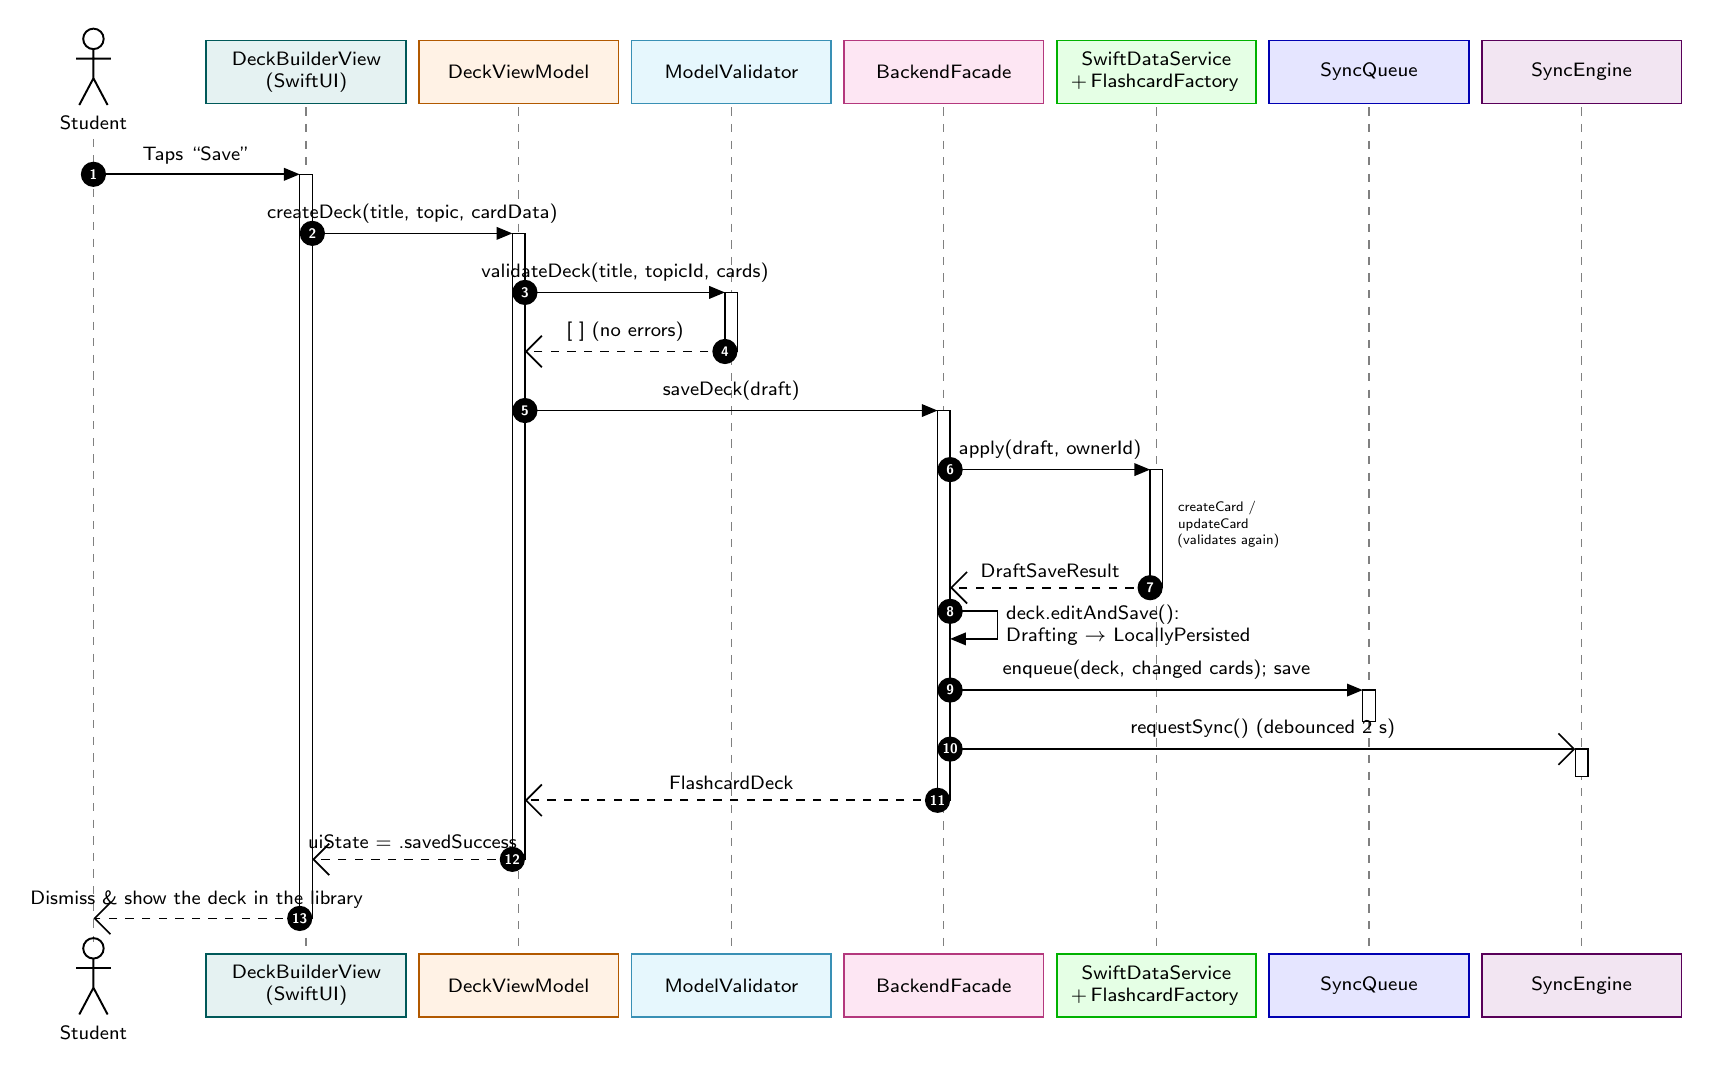
\begin{tikzpicture}[font=\sffamily\scriptsize]
  % Lifeline x-positions
  \def\xS{0}\def\xV{2.7}\def\xM{5.4}\def\xA{8.1}\def\xF{10.8}\def\xD{13.5}\def\xQ{16.2}\def\xE{18.9}
  \def\ytop{0}\def\ybot{-11.6}
  % Heads
  \pic at (\xS,\ytop) {stickman};
  \node at (\xS,\ytop-0.65) {Student};
  \foreach \x/\n/\c in {\xV/{DeckBuilderView\\(SwiftUI)}/teal,
                        \xM/DeckViewModel/orange,
                        \xA/ModelValidator/cyan,
                        \xF/BackendFacade/magenta,
                        \xD/{SwiftDataService\\+\,FlashcardFactory}/green,
                        \xQ/SyncQueue/blue,
                        \xE/SyncEngine/violet}{
    \node[draw=\c!70!black, fill=\c!10, align=center, minimum height=0.8cm,
          text width=2.3cm, line width=0.6pt] at (\x,\ytop) {\n};
    \node[draw=\c!70!black, fill=\c!10, align=center, minimum height=0.8cm,
          text width=2.3cm, line width=0.6pt] at (\x,\ybot) {\n};
    \draw[dashed, gray] (\x,\ytop-0.45) -- (\x,\ybot+0.45);
  }
  \draw[dashed, gray] (\xS,\ytop-0.85) -- (\xS,\ybot+0.55);
  \pic at (\xS,\ybot+0.05) {stickman};
  \node at (\xS,\ybot-0.6) {Student};
  % Activation bars
  \foreach \x/\a/\b in {\xV/-1.3/-10.75, \xM/-2.05/-10.0, \xA/-2.8/-3.55,
                        \xF/-4.3/-9.25, \xD/-5.05/-6.55, \xQ/-7.85/-8.25, \xE/-8.6/-8.95}{
    \fill[white] (\x-0.08,\a) rectangle (\x+0.08,\b);
    \draw[line width=0.5pt] (\x-0.08,\a) rectangle (\x+0.08,\b);
  }
  % Messages: \msg{step}{from x}{to x}{y}{label}{style}
  \newcommand{\msg}[6]{%
    \draw[#6] (#2,#4) -- node[above=2.5pt, inner sep=1pt] {#5} (#3,#4);
    \node[circle, fill=black, text=white, inner sep=0.5pt, minimum size=3.2mm,
          font=\sffamily\tiny\bfseries] at (#2,#4) {#1};}
  % Self message: \self{step}{x}{y}{label}
  \newcommand{\selfmsg}[4]{%
    \draw[sync] (#2+0.08,#3) -- ++(0.6,0) -- ++(0,-0.35) -- (#2+0.08,#3-0.35);
    \node[anchor=west, inner sep=1pt, align=left] at (#2+0.75,#3-0.17) {#4};
    \node[circle, fill=black, text=white, inner sep=0.5pt, minimum size=3.2mm,
          font=\sffamily\tiny\bfseries] at (#2+0.08,#3) {#1};}
  \tikzset{sync/.style={line width=0.6pt, -{Triangle[length=2mm,width=1.6mm]}},
           ret/.style={line width=0.6pt, dashed, -{Straight Barb[length=2mm]}},
           async/.style={line width=0.6pt, -{Straight Barb[length=2mm]}}}
  \msg{1}{\xS}{\xV-0.08}{-1.3}{Taps ``Save''}{sync}
  \msg{2}{\xV+0.08}{\xM-0.08}{-2.05}{createDeck(title, topic, cardData)}{sync}
  \msg{3}{\xM+0.08}{\xA-0.08}{-2.8}{validateDeck(title, topicId, cards)}{sync}
  \msg{4}{\xA-0.08}{\xM+0.08}{-3.55}{[ ] (no errors)}{ret}
  \msg{5}{\xM+0.08}{\xF-0.08}{-4.3}{saveDeck(draft)}{sync}
  \msg{6}{\xF+0.08}{\xD-0.08}{-5.05}{apply(draft, ownerId)}{sync}
  \node[align=left, anchor=west, font=\sffamily\tiny, text width=2.2cm] at (\xD+0.15,-5.75) {createCard /\\updateCard\\(validates again)};
  \msg{7}{\xD-0.08}{\xF+0.08}{-6.55}{DraftSaveResult}{ret}
  \selfmsg{8}{\xF}{-6.85}{deck.editAndSave():\\Drafting $\to$ LocallyPersisted}
  \msg{9}{\xF+0.08}{\xQ-0.08}{-7.85}{enqueue(deck, changed cards); save}{sync}
  \msg{10}{\xF+0.08}{\xE-0.08}{-8.6}{requestSync() (debounced 2 s)}{async}
  \msg{11}{\xF-0.08}{\xM+0.08}{-9.25}{FlashcardDeck}{ret}
  \msg{12}{\xM-0.08}{\xV+0.08}{-10.0}{uiState = .savedSuccess}{ret}
  \msg{13}{\xV-0.08}{\xS}{-10.75}{Dismiss \& show the deck in the library}{ret}
\end{tikzpicture}}
\caption{UML sequence diagram: Create Flashcard Deck via in-app form (UC-01)}
\label{fig:sequence}
\end{figure}

Figure~\ref{fig:sequence} models the main success scenario of UC-01. The student
edits the draft and selects \emph{Save} (1). \texttt{DeckBuilderView} calls
\texttt{DeckViewModel.save()}, which calls \texttt{createDeck(title, topic,
cardData)} for a new deck (2). The view model validates the whole draft with
\texttt{ModelValidator} (3); an empty list of field errors means the draft is valid
(4). The view model then passes the draft to \texttt{BackendFacade.saveDeck()} (5),
the only backend operation it depends on (through the \texttt{DeckBackend} protocol).
The facade asks \texttt{SwiftDataService} to apply the draft (6). It creates or
updates every card through \texttt{FlashcardFactory}, which validates the content a
second time, so no card can bypass the rules. \texttt{SwiftDataService} reports which
cards changed (7). The deck takes the \emph{edit} and \emph{save} transitions of the
State pattern into \emph{LocallyPersisted} (8). The facade queues the deck and its
changed cards, saves the store (9), and asks \texttt{SyncEngine} for a sync two
seconds later (10), so replication runs in the background and rapid saves share one
push. The facade returns the saved deck (11), the view model publishes
\texttt{savedSuccess} (12), and the view dismisses the form (13).

The deck is persisted locally before any network activity (FR-44), which enables
offline deck creation (NFR-08). If validation fails at step 4, the view model stores
the field errors, the view moves to the first invalid card, and the flow stops before
the facade is called (FR-10).

\begin{figure}[!htbp]
\centering
\resizebox{\textwidth}{!}{%
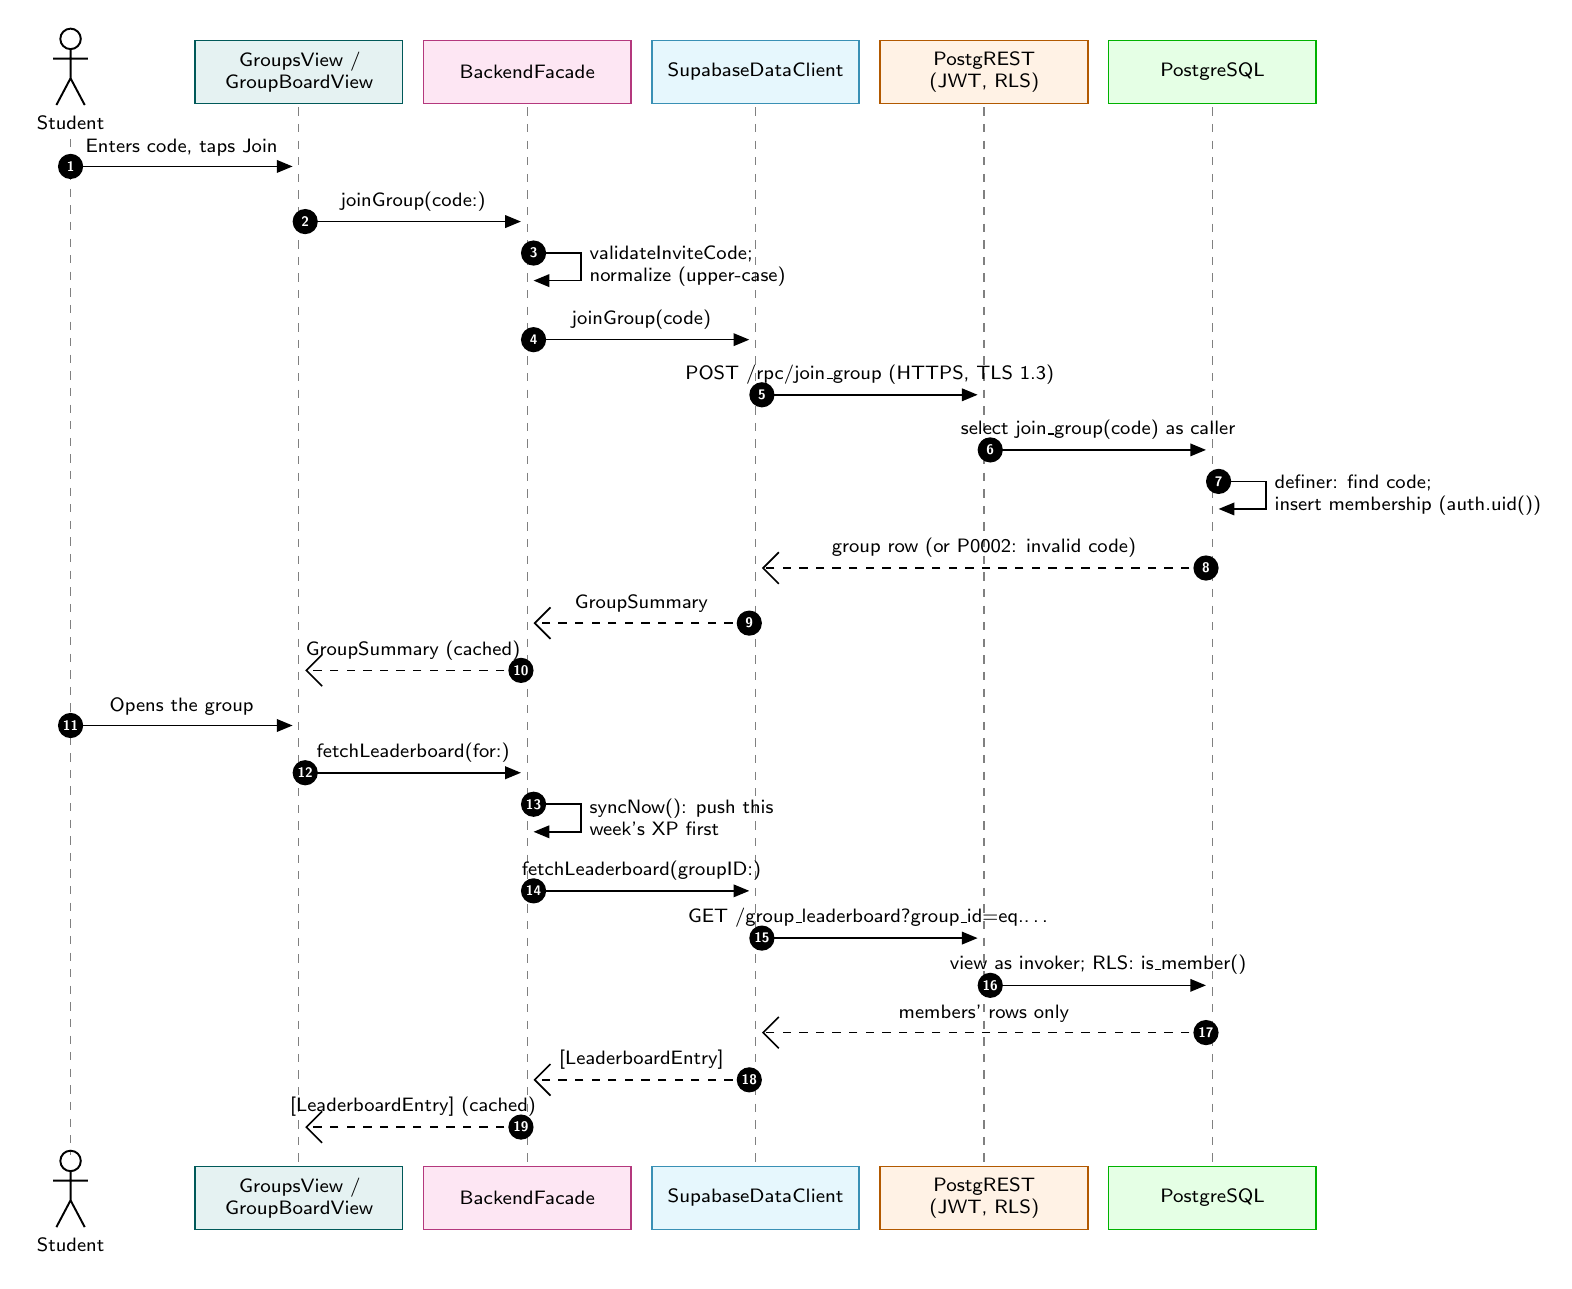
\begin{tikzpicture}[font=\sffamily\scriptsize]
  \def\xS{0}\def\xV{2.9}\def\xF{5.8}\def\xC{8.7}\def\xR{11.6}\def\xP{14.5}
  \def\ytop{0}\def\ybot{-14.3}
  \pic at (\xS,\ytop) {stickman};
  \node at (\xS,\ytop-0.65) {Student};
  \foreach \x/\n/\c in {\xV/{GroupsView /\\GroupBoardView}/teal,
                        \xF/BackendFacade/magenta,
                        \xC/SupabaseDataClient/cyan,
                        \xR/{PostgREST\\(JWT, RLS)}/orange,
                        \xP/{PostgreSQL}/green}{
    \node[draw=\c!70!black, fill=\c!10, align=center, minimum height=0.8cm,
          text width=2.4cm, line width=0.6pt] at (\x,\ytop) {\n};
    \node[draw=\c!70!black, fill=\c!10, align=center, minimum height=0.8cm,
          text width=2.4cm, line width=0.6pt] at (\x,\ybot) {\n};
    \draw[dashed, gray] (\x,\ytop-0.45) -- (\x,\ybot+0.45);
  }
  \draw[dashed, gray] (\xS,\ytop-0.85) -- (\xS,\ybot+0.55);
  \pic at (\xS,\ybot+0.05) {stickman};
  \node at (\xS,\ybot-0.6) {Student};
  \tikzset{sync/.style={line width=0.6pt, -{Triangle[length=2mm,width=1.6mm]}},
           ret/.style={line width=0.6pt, dashed, -{Straight Barb[length=2mm]}}}
  \newcommand{\gmsg}[6]{%
    \draw[#6] (#2,#4) -- node[above=2.5pt, inner sep=1pt] {#5} (#3,#4);
    \node[circle, fill=black, text=white, inner sep=0.5pt, minimum size=3.2mm,
          font=\sffamily\tiny\bfseries] at (#2,#4) {#1};}
  \newcommand{\gself}[4]{%
    \draw[sync] (#2+0.08,#3) -- ++(0.6,0) -- ++(0,-0.35) -- (#2+0.08,#3-0.35);
    \node[anchor=west, inner sep=1pt, align=left] at (#2+0.75,#3-0.17) {#4};
    \node[circle, fill=black, text=white, inner sep=0.5pt, minimum size=3.2mm,
          font=\sffamily\tiny\bfseries] at (#2+0.08,#3) {#1};}
  \gmsg{1}{\xS}{\xV-0.08}{-1.2}{Enters code, taps Join}{sync}
  \gmsg{2}{\xV+0.08}{\xF-0.08}{-1.9}{joinGroup(code:)}{sync}
  \gself{3}{\xF}{-2.3}{validateInviteCode;\\normalize (upper-case)}
  \gmsg{4}{\xF+0.08}{\xC-0.08}{-3.4}{joinGroup(code)}{sync}
  \gmsg{5}{\xC+0.08}{\xR-0.08}{-4.1}{POST /rpc/join\_group (HTTPS, TLS 1.3)}{sync}
  \gmsg{6}{\xR+0.08}{\xP-0.08}{-4.8}{select join\_group(code) as caller}{sync}
  \gself{7}{\xP}{-5.2}{definer: find code;\\insert membership (auth.uid())}
  \gmsg{8}{\xP-0.08}{\xC+0.08}{-6.3}{group row (or P0002: invalid code)}{ret}
  \gmsg{9}{\xC-0.08}{\xF+0.08}{-7.0}{GroupSummary}{ret}
  \gmsg{10}{\xF-0.08}{\xV+0.08}{-7.6}{GroupSummary (cached)}{ret}
  \gmsg{11}{\xS}{\xV-0.08}{-8.3}{Opens the group}{sync}
  \gmsg{12}{\xV+0.08}{\xF-0.08}{-8.9}{fetchLeaderboard(for:)}{sync}
  \gself{13}{\xF}{-9.3}{syncNow(): push this\\week's XP first}
  \gmsg{14}{\xF+0.08}{\xC-0.08}{-10.4}{fetchLeaderboard(groupID:)}{sync}
  \gmsg{15}{\xC+0.08}{\xR-0.08}{-11.0}{GET /group\_leaderboard?group\_id=eq.\ldots}{sync}
  \gmsg{16}{\xR+0.08}{\xP-0.08}{-11.6}{view as invoker; RLS: is\_member()}{sync}
  \gmsg{17}{\xP-0.08}{\xC+0.08}{-12.2}{members' rows only}{ret}
  \gmsg{18}{\xC-0.08}{\xF+0.08}{-12.8}{[LeaderboardEntry]}{ret}
  \gmsg{19}{\xF-0.08}{\xV+0.08}{-13.4}{[LeaderboardEntry] (cached)}{ret}
\end{tikzpicture}}
\caption{UML sequence diagram: join a group by invite code, then load its weekly leaderboard (UC-21, UC-22)}
\label{fig:sequence2}
\end{figure}

Figure~\ref{fig:sequence2} shows how group data crosses the trust boundary. The
student enters an invite code (1); the view calls the facade (2), which validates the
format and upper-cases it (3) before any request, then calls the adapter (4). The
adapter makes the app's only remote procedure call, \texttt{join\_group} (5). PostgREST
runs it as the signed-in caller (6). The function is \texttt{SECURITY DEFINER} with an
empty search path, so it can look up a code in a group the caller cannot yet see,
and it inserts exactly one membership row for \texttt{auth.uid()} (7); the caller
cannot pass a different user. An unknown code raises an error that the adapter maps
to ``No group has that code'' (8). The group is returned and cached for offline display
(9, 10). Opening the group (11, 12) first pushes the student's weekly XP so their own
row is current (13), then asks the adapter to read the \texttt{group\_leaderboard} view
(14, 15); like every remote call, it goes through \texttt{SupabaseDataClient}, the only
type that talks to Supabase (risk R7). The view is \texttt{security\_invoker}, so the
caller's Row Level Security applies: only groups the caller belongs to return rows
(16, 17), which is what NFR-25 requires. The adapter maps the rows to
\texttt{LeaderboardEntry} values (18), and the facade caches the board for offline
display before returning it (19). Steps 2--19 run
only when the student is signed in and online; otherwise the last cached board is shown
(the flows of UC-22).

% =====================================================================
\begin{figure}[!htbp]
\centering
\resizebox{\textwidth}{!}{%
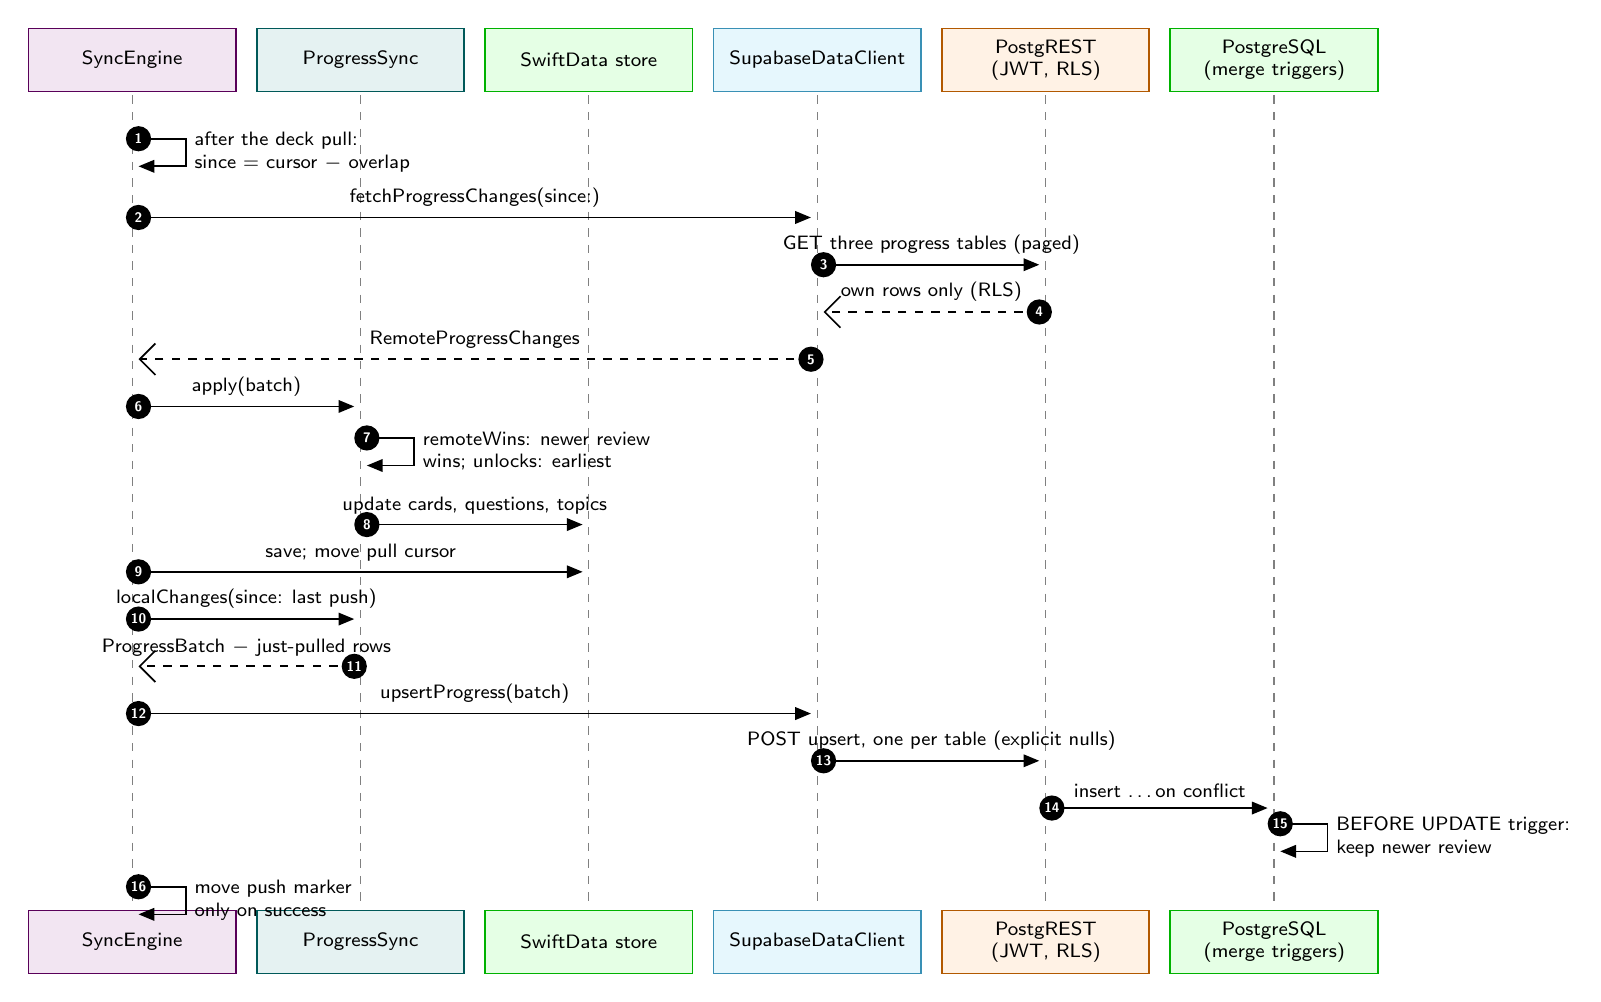
\begin{tikzpicture}[font=\sffamily\scriptsize]
  \def\xE{0}\def\xG{2.9}\def\xL{5.8}\def\xC{8.7}\def\xR{11.6}\def\xP{14.5}
  \def\ytop{0}\def\ybot{-11.2}
  \foreach \x/\n/\c in {\xE/SyncEngine/violet,
                        \xG/ProgressSync/teal,
                        \xL/{SwiftData store}/green,
                        \xC/SupabaseDataClient/cyan,
                        \xR/{PostgREST\\(JWT, RLS)}/orange,
                        \xP/{PostgreSQL\\(merge triggers)}/green}{
    \node[draw=\c!70!black, fill=\c!10, align=center, minimum height=0.8cm,
          text width=2.4cm, line width=0.6pt] at (\x,\ytop) {\n};
    \node[draw=\c!70!black, fill=\c!10, align=center, minimum height=0.8cm,
          text width=2.4cm, line width=0.6pt] at (\x,\ybot) {\n};
    \draw[dashed, gray] (\x,\ytop-0.45) -- (\x,\ybot+0.45);
  }
  \tikzset{sync/.style={line width=0.6pt, -{Triangle[length=2mm,width=1.6mm]}},
           ret/.style={line width=0.6pt, dashed, -{Straight Barb[length=2mm]}}}
  \newcommand{\pmsg}[6]{%
    \draw[#6] (#2,#4) -- node[above=2.5pt, inner sep=1pt] {#5} (#3,#4);
    \node[circle, fill=black, text=white, inner sep=0.5pt, minimum size=3.2mm,
          font=\sffamily\tiny\bfseries] at (#2,#4) {#1};}
  \newcommand{\pself}[4]{%
    \draw[sync] (#2+0.08,#3) -- ++(0.6,0) -- ++(0,-0.35) -- (#2+0.08,#3-0.35);
    \node[anchor=west, inner sep=1pt, align=left] at (#2+0.75,#3-0.17) {#4};
    \node[circle, fill=black, text=white, inner sep=0.5pt, minimum size=3.2mm,
          font=\sffamily\tiny\bfseries] at (#2+0.08,#3) {#1};}
  \pself{1}{\xE}{-1.0}{after the deck pull:\\since = cursor $-$ overlap}
  \pmsg{2}{\xE+0.08}{\xC-0.08}{-2.0}{fetchProgressChanges(since:)}{sync}
  \pmsg{3}{\xC+0.08}{\xR-0.08}{-2.6}{GET three progress tables (paged)}{sync}
  \pmsg{4}{\xR-0.08}{\xC+0.08}{-3.2}{own rows only (RLS)}{ret}
  \pmsg{5}{\xC-0.08}{\xE+0.08}{-3.8}{RemoteProgressChanges}{ret}
  \pmsg{6}{\xE+0.08}{\xG-0.08}{-4.4}{apply(batch)}{sync}
  \pself{7}{\xG}{-4.8}{remoteWins: newer review\\wins; unlocks: earliest}
  \pmsg{8}{\xG+0.08}{\xL-0.08}{-5.9}{update cards, questions, topics}{sync}
  \pmsg{9}{\xE+0.08}{\xL-0.08}{-6.5}{save; move pull cursor}{sync}
  \pmsg{10}{\xE+0.08}{\xG-0.08}{-7.1}{localChanges(since: last push)}{sync}
  \pmsg{11}{\xG-0.08}{\xE+0.08}{-7.7}{ProgressBatch $-$ just-pulled rows}{ret}
  \pmsg{12}{\xE+0.08}{\xC-0.08}{-8.3}{upsertProgress(batch)}{sync}
  \pmsg{13}{\xC+0.08}{\xR-0.08}{-8.9}{POST upsert, one per table (explicit nulls)}{sync}
  \pmsg{14}{\xR+0.08}{\xP-0.08}{-9.5}{insert \ldots on conflict}{sync}
  \pself{15}{\xP}{-9.7}{BEFORE UPDATE trigger:\\keep newer review}
  \pself{16}{\xE}{-10.5}{move push marker\\only on success}
\end{tikzpicture}}
\caption{UML sequence diagram: study-progress step of a sync cycle (FR-61)}
\label{fig:sequence3}
\end{figure}

Figure~\ref{fig:sequence3} shows the progress step that \texttt{SyncEngine} runs in
every sync cycle after decks are pulled, so a pulled card exists before its progress
arrives (1). It asks for progress rows changed since the last pull, minus a 2-second
overlap so rows committed at the same moment are not missed (2--5); Row Level Security returns only the
student's own rows. \texttt{ProgressSync} applies the merge rules (6, 7): a remote
review replaces the local one only if it is strictly newer, and a tier unlock keeps
the earlier date, so an unlock is never lost. The changes are saved and the pull cursor
moves (8, 9). Then the rows reviewed on this device since the last successful push
are collected, without the rows just pulled, so nothing is echoed back (10, 11), and
pushed in one upsert per table (12, 13). Optional columns are sent as explicit nulls:
an omitted \texttt{retired\_at} would leave a stale value on the server (the interface
fault in Section~\ref{sec:integration}). The database applies the same ``newer review
wins'' rule in a trigger (14, 15), so two devices converge whichever pushes first.
The push marker moves only after a successful push (16), so a failed cycle resends
its rows next time. Progress does not use the change queue (decision S32): rows are
compared by timestamp each cycle instead.

\section{UML State Diagram (Updated for Sprint 4)}
% =====================================================================
The deck synchronization lifecycle is unchanged since Sprint 2 and remains the
specification of the State pattern. Sprint 4 added no new state machine: study progress
(FR-61) is merged by timestamp in every sync cycle rather than moving through states,
and an exercise has only two screen states (answering and checked), which are local
view state and are never stored.


\begin{figure}[!htbp]
\centering
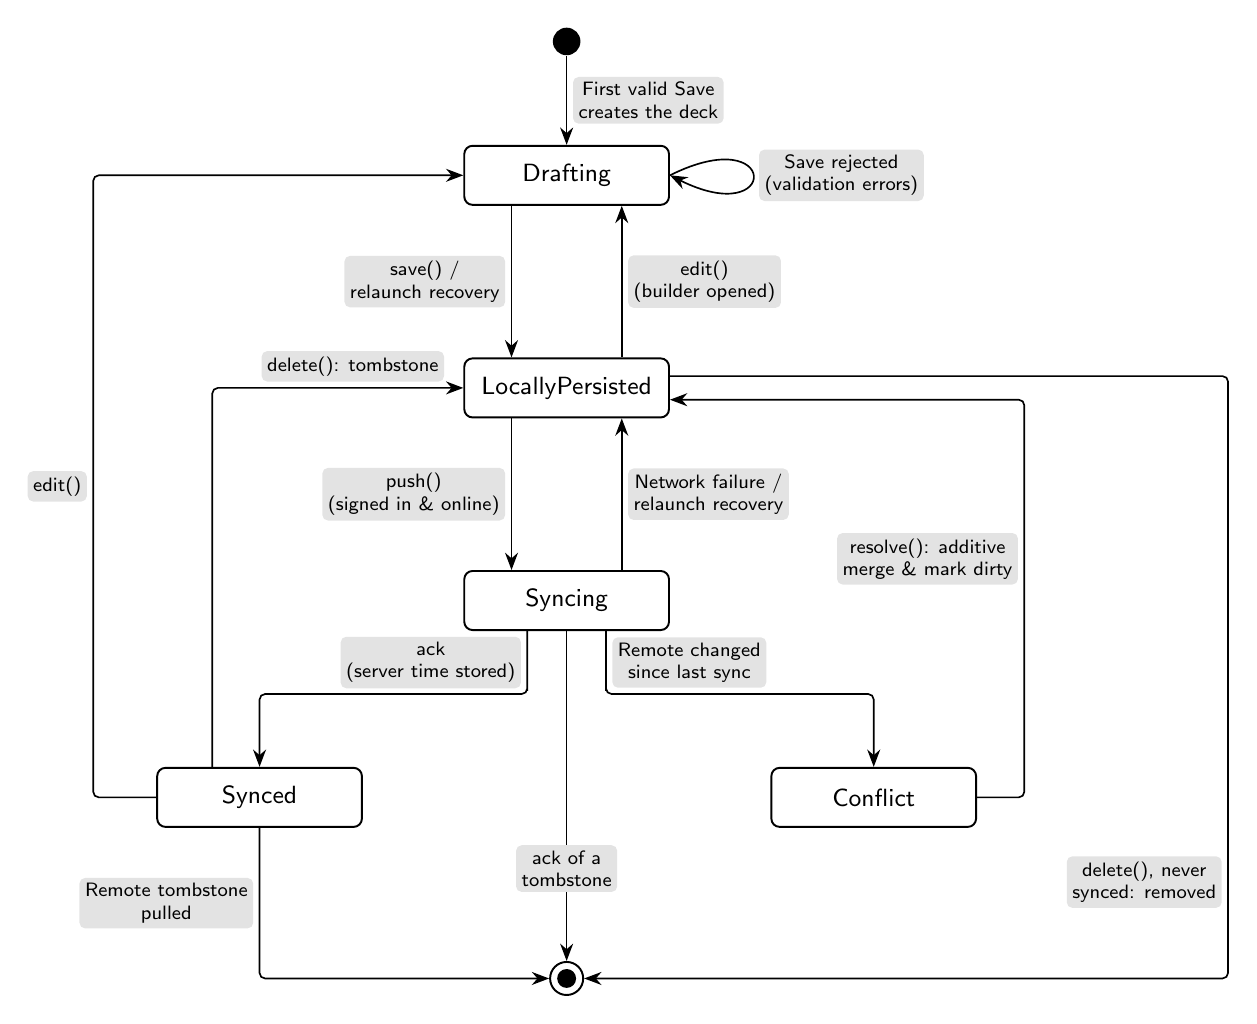
\begin{tikzpicture}[font=\sffamily\scriptsize]
  % States
  \node[circle, fill=black, minimum size=3.5mm, inner sep=0pt] (init) at (0,0) {};
  \node[state] (draft) at (0,-1.7)  {Drafting};
  \node[state] (lp)    at (0,-4.4)  {LocallyPersisted};
  \node[state] (sync)  at (0,-7.1)  {Syncing};
  \node[state] (done)  at (-3.9,-9.6){Synced};
  \node[state] (conf)  at (3.9,-9.6) {Conflict};
  \node[circle, draw, line width=0.7pt, minimum size=4.2mm, inner sep=0pt] (fin) at (0,-11.9) {};
  \node[circle, fill=black, minimum size=2.4mm, inner sep=0pt] at (fin) {};
  % Transitions
  \draw[trans] (init) -- node[glbl, right=2pt] {First valid Save\\creates the deck} (draft);
  \draw[trans] (draft.east) .. controls +(1.4,0.7) and +(1.4,-0.7) ..
        node[glbl, right=2pt] {Save rejected\\(validation errors)} (draft.east);
  \draw[trans] ([xshift=-7mm]draft.south) -- node[glbl, left=2pt] {save() /\\relaunch recovery} ([xshift=-7mm]lp.north);
  \draw[trans] ([xshift=7mm]lp.north) -- node[glbl, right=2pt] {edit()\\(builder opened)} ([xshift=7mm]draft.south);
  \draw[trans] ([xshift=-7mm]lp.south) -- node[glbl, left=2pt] {push()\\(signed in \& online)} ([xshift=-7mm]sync.north);
  \draw[trans] ([xshift=7mm]sync.north) -- node[glbl, right=2pt] {Network failure /\\relaunch recovery} ([xshift=7mm]lp.south);
  \draw[trans] ([xshift=-5mm]sync.south) |- node[glbl, pos=0.25, left=2pt] {ack\\(server time stored)} ++(0,-0.8) -| (done.north);
  \draw[trans] ([xshift=5mm]sync.south)  |- node[glbl, pos=0.25, right=2pt] {Remote changed\\since last sync} ++(0,-0.8) -| (conf.north);
  \draw[trans] (sync.south) -- node[glbl, pos=0.72] {ack of a\\tombstone} (fin.north);
  \draw[trans] (conf.east) -- ++(0.6,0) |- node[glbl, pos=0.3, left=2pt] {resolve(): additive\\merge \& mark dirty} ([yshift=-1.5mm]lp.east);
  \draw[trans] (done.west) -- ++(-0.8,0) |- node[glbl, pos=0.25, left=2pt] {edit()} (draft.west);
  \draw[trans] ([xshift=-6mm]done.north) |- node[glbl, pos=0.78, above=2pt] {delete(): tombstone} (lp.west);
  \draw[trans] ([yshift=1.5mm]lp.east) -- (8.4,-4.25) |- node[glbl, pos=0.42, left=2pt] {delete(), never\\synced: removed} (fin.east);
  \draw[trans] (done.south) |- node[glbl, pos=0.25, left=2pt] {Remote tombstone\\pulled} (fin.west);
\end{tikzpicture}
\caption{UML state diagram: FlashcardDeck sync lifecycle}
\label{fig:state}
\end{figure}

Figure~\ref{fig:state} models the lifecycle of a user-created \texttt{FlashcardDeck}
across five states: \emph{Drafting}, \emph{LocallyPersisted}, \emph{Syncing},
\emph{Synced}, and \emph{Conflict}. The deck model is created by its first valid save;
while a new deck is being written, the builder edits an in-memory draft, so a save that
fails validation leaves no deck behind and an existing deck stays in \emph{Drafting}.

A valid save moves the deck to \emph{LocallyPersisted}. When the student is signed in
and online, \texttt{SyncEngine} pushes it, moving it to \emph{Syncing}. A network
failure returns it to \emph{LocallyPersisted} for a retry with exponential backoff, so
no local changes are lost. A successful acknowledgment stores the server's update
timestamp and moves the deck to \emph{Synced}. If that timestamp has moved past the one
stored at the last sync, another device changed the deck, and it moves to
\emph{Conflict}. There the additive merge runs, and \texttt{resolve()} marks the deck
dirty and returns it to \emph{LocallyPersisted}, from which it is pushed again in the
same sync cycle. Editing a synced deck returns it to \emph{Drafting}.

Two recovery transitions run at app launch, so that a deck is never stranded: a deck
left in \emph{Syncing} by a terminated app returns to \emph{LocallyPersisted}, and so
does a deck persisted in \emph{Drafting}. A deck left in \emph{Conflict} is merged
again on the next push.

A deck may be deleted only from \emph{LocallyPersisted} or \emph{Synced}; deletion is
unavailable in \emph{Drafting}, \emph{Syncing}, and \emph{Conflict}, which prevents
orphaned remote records. A deck that has never synced is removed at once. A deck that
has synced before becomes a tombstone in \emph{LocallyPersisted} (a \emph{Synced} deck
moves there), and a delete operation is queued; the deck is removed when the server
acknowledges the tombstone (FR-12). A tombstone pulled from another device removes a
\emph{Synced} deck. Starter decks (FR-15) never enter this lifecycle: they cannot be
edited, deleted, or pushed, only hidden.

This diagram is the specification for the State pattern (Section~\ref{sec:state}).
Each state is implemented as a type, each transition as the return value of an
\texttt{on\ldots()} method, and each transition and each disallowed operation is
covered by a unit test (risk R9).

% =====================================================================
\section{UML Class Diagrams and Design Patterns (Updated for Sprint 4)}
% =====================================================================
Section~\ref{sec:domain} presents the core domain model and its Sprint 3 and Sprint 4
additions,
Sections~\ref{sec:factory} through~\ref{sec:facade} present one Gang of Four design
pattern from each category, and Section~\ref{sec:patternmap} maps every pattern
participant to its source lines in Appendix~B. Visibility is denoted by \texttt{+} (public), \texttt{-}
(private), and \texttt{\#} (protected).

\subsection{Core Domain Model}\label{sec:domain}
\begin{figure}[!htbp]
\centering
\begin{tikzpicture}
  \node[cls={orange}{6.0cm}] (vm) at (-3.0,0) {\ctitle{\textbf{DeckViewModel}}
    \nodepart{two}\raggedright +draft: DeckDraft\\ +fieldErrors: [ValidationField: String]\\ +uiState: UIState\\ \priv backend: DeckBackend
    \nodepart{three}\raggedright +createDeck(title, topic, cardData) : FlashcardDeck?\\ +updateDeck() : FlashcardDeck?\\ +save() : FlashcardDeck?\\ +addCard(after: UUID?) : UUID\\ +deleteCard(cardID: UUID)\\ +validateNow() : [FieldError]\\ (also duplicate, restore, move, toggleSnippet)};
  \node[cls={gray}{4.6cm}] (db) at (3.9,0.6) {\ctitle{\st{interface}\\\textbf{DeckBackend}}
    \nodepart{two}~
    \nodepart{three}\raggedright +saveDeck(draft) : FlashcardDeck\\ +deleteDeck(deck)\\ +setHidden(hidden, deck)};
  \node[cls={violet}{4.6cm}, anchor=north] (bf) at (3.9,-1.6) {\ctitle{\textbf{BackendFacade}}\nodepart{two}~\nodepart{three}\raggedright see Fig.~\ref{fig:facade}};
  \node[cls={magenta}{5.6cm}, anchor=north] (deck) at (-3.0,-5.0) {\ctitle{\textbf{FlashcardDeck}}
    \nodepart{two}\raggedright +id: UUID\\ +title: String\\ +topicId: String\\ +origin: DeckOrigin\\ +isHidden: Bool\\ +ownerId: UUID?\\ +syncState: DeckSyncStateKind\\ +deletedAt: Date?
    \nodepart{three}\raggedright +activeCards: [Flashcard] \{get\}\\ +cardCount: Int \{get\}\\ +masteryRate: Double \{get\}\\ +progressRate: Double \{get\}\\ \textasciitilde markDirty(at: Date)};
  \node[cls={cyan}{4.6cm}, anchor=north] (sds) at (3.9,-5.0) {\ctitle{\textbf{SwiftDataService}}
    \nodepart{two}\raggedright \priv context: ModelContext\\ \priv factory: FlashcardFactory
    \nodepart{three}\raggedright +apply(draft, ownerId) : DraftSaveResult\\ +fetch(id: UUID) : FlashcardDeck?\\ +fetchCard(id: UUID) : Flashcard?};
  \node[cls={teal}{5.6cm}, anchor=north] (card) at (-3.0,-11.0) {\ctitle{\textbf{Flashcard}}
    \nodepart{two}\raggedright +id: UUID\\ +prompt: String\\ +answer: String\\ +codeSnippet: CodeSnippet?\\ +difficulty: Difficulty?\\ +sortIndex: Int\\ +masteryScore: Int \{readOnly\}\\ +retiredAt: Date?
    \nodepart{three}\raggedright +updateMastery(rating: CardRating)\\ +resetMastery()\\ +toPayload() : FlashcardPayload};
  \node[cls={green}{4.0cm}, anchor=north] (cs) at (3.9,-11.0) {\ctitle{\st{struct}\\\textbf{CodeSnippet}}
    \nodepart{two}\raggedright +language: CodeLanguage\\ +source: String
    \nodepart{three}~};
  \draw[dep] (vm.east |- db.west) -- node[lbl] {\st{use}} (db.west);
  \draw[realize] (bf.north) -- (db.south);
  \draw[dep] (bf.south) -- node[lbl] {\st{use}} (sds.north);
  \draw[dep] (sds.west |- deck.north east) ++(0,-0.6) coordinate (p) (sds.west |- p) -- node[lbl] {\st{create}} (deck.east |- p);
  \draw[compo] (deck.south) -- node[lbl] {contains} (card.north)
        node[pos=0.12, right, font=\sffamily\scriptsize] {1}
        node[pos=0.88, right, font=\sffamily\scriptsize] {0..*};
  \draw[compo] (card.east |- cs.north west) ++(0,-0.5) coordinate (q) (card.east |- q) -- (cs.west |- q)
        node[pos=0.85, above, font=\sffamily\scriptsize] {0..1};
\end{tikzpicture}
\caption{UML class diagram: core domain model}
\label{fig:domain}
\end{figure}

\texttt{FlashcardDeck} owns its \texttt{Flashcard} instances through composition
(1 to 0..*): a card cannot exist without its deck, and deleting a deck deletes its
cards. A card owns at most one \texttt{CodeSnippet}, a value type stored with the card.
\texttt{DeckViewModel} (an \texttt{@Observable} class) edits an in-memory
\texttt{DeckDraft} rather than the stored deck, so an abandoned edit never touches the
store. It depends only on the \texttt{DeckBackend} protocol, which
\texttt{BackendFacade} implements, so its unit tests run against the real facade in
local-only mode with no network. The facade applies a saved draft through
\texttt{SwiftDataService}, which creates and updates cards through
\texttt{FlashcardFactory} (Section~\ref{sec:factory}).

\texttt{FlashcardDeck} stores a \texttt{topicId} that refers to the predefined topic
list, together with its \texttt{origin} (user or starter), \texttt{isHidden},
\texttt{ownerId}, and a \texttt{deletedAt} tombstone for synchronization. Its card
count and mastery rate are computed properties. Cards are attached through the
composition relationship, so no \texttt{addCard()} operation is needed. Validation
lives in \texttt{ModelValidator}, which the factory calls for every card, rather than
in the model classes. A card's payload is a typed \texttt{FlashcardPayload}, and mastery
changes take a \texttt{CardRating}.

\begin{figure}[!htbp]
\centering
\resizebox{\textwidth}{!}{%
\begin{tikzpicture}
  \node[cls={magenta}{5.0cm}] (prof) at (-5.2,0) {\ctitle{\st{V7 model}\\\textbf{UserProfile}}
    \nodepart{two}\raggedright +username: String (display name)\\ +avatarId: String?\\ +totalXP: Int\\ +pinnedTopicIds: [String]
    \nodepart{three}\raggedright +level: Int \{get\}};
  \node[cls={magenta}{4.4cm}] (award) at (0.4,0) {\ctitle{\st{V7 model}\\\textbf{BadgeAward}}
    \nodepart{two}\raggedright +badgeRaw: String \{unique\}\\ +earnedAt: Date
    \nodepart{three}~};
  \node[cls={gray}{4.4cm}] (badge) at (5.6,0) {\ctitle{\st{enum}\\\textbf{Badge}}
    \nodepart{two}\raggedright firstDeck, sevenDayStreak,\\ xp1000, weeklyChallenge
    \nodepart{three}~};
  \node[cls={orange}{5.0cm}, anchor=north] (be) at (5.6,-2.6) {\ctitle{\st{enum}\\\textbf{BadgeEvaluator}}
    \nodepart{two}~
    \nodepart{three}\raggedright +qualifying(facts) : Set$<$Badge$>$\\ +award(context: ModelContext)};
  \node[cls={orange}{5.4cm}, anchor=north] (sc) at (-5.2,-3.4) {\ctitle{\st{enum}\\\textbf{StreakCalculator}}
    \nodepart{two}~
    \nodepart{three}\raggedright +isGoalMet(day: DailyActivity) : Bool\\ +currentStreak(endingOn, activity, calendar) : Int};
  \node[cls={teal}{4.4cm}, anchor=north] (da) at (-5.2,-6.4) {\ctitle{\st{V3 model}\\\textbf{DailyActivity}}
    \nodepart{two}\raggedright +day: String\\ +quizAnswers: Int\\ +cardsRated: Int
    \nodepart{three}~};
  \node[cls={orange}{5.0cm}, anchor=north] (wc) at (0.4,-3.8) {\ctitle{\st{enum}\\\textbf{WeeklyChallenge}}
    \nodepart{two}\raggedright +goal = 15
    \nodepart{three}\raggedright +topicID(for: Date, topicIDs) : String?\\ +status(now, topicIDs, records) : Status?};
  \node[cls={teal}{4.4cm}, anchor=north] (qa) at (0.4,-6.8) {\ctitle{\st{V4 model}\\\textbf{QuizAnswerRecord}}
    \nodepart{two}\raggedright +topicId: String\\ +correct: Bool\\ +answeredAt: Date
    \nodepart{three}~};
  \node[cls={cyan}{4.4cm}, anchor=north] (gs) at (5.6,-5.9) {\ctitle{\st{struct}\\\textbf{GroupSummary}}
    \nodepart{two}\raggedright +id: UUID\\ +name: String\\ +inviteCode: String
    \nodepart{three}~};
  \node[cls={cyan}{4.4cm}, anchor=north] (le) at (5.6,-8.6) {\ctitle{\st{struct}\\\textbf{LeaderboardEntry}}
    \nodepart{two}\raggedright +userId: UUID\\ +displayName: String\\ +avatarId: String?\\ +xp: Int
    \nodepart{three}~};
  \draw[dep] (sc.south) -- node[lbl] {\st{use}} (da.north);
  \draw[dep] (wc.south) -- node[lbl] {\st{use}} (qa.north);
  \draw[dep] (be.west) -| node[lbl, pos=0.25] {\st{create}} (award.south);
  \draw[dep] (badge.south) -- node[lbl] {evaluates} (be.north);
  \draw[dep] (be.west) ++(0,-0.5) coordinate (bw) (bw) -- (wc.east |- bw);
  \draw[dep] (gs.south) -- node[lbl] {board of} (le.north);
\end{tikzpicture}}
\caption{UML class diagram: Sprint 3 domain additions (gamification and groups)}
\label{fig:domain3}
\end{figure}

Figure~\ref{fig:domain3} shows the types Sprint 3 added. Persisted state changed
in two schema versions. Version 7 removes the unused stored streak from
\texttt{UserProfile}, adds \texttt{avatarId} (FR-60), and adds \texttt{BadgeAward}, one
row per earned badge with its date, so a badge stays earned after the data behind it
changes. Version 8 (the study-session fix) lets \texttt{StudyProgressSnapshot} keep
each card's mastery score and the deck's progress at the start of a session, so the
summary can report the cards that moved up; \texttt{FlashcardDeck.progressRate} (the
sum of the cards' scores over five times the card count) is computed, not stored, as
is everything else in the figure. \texttt{StreakCalculator} derives the daily goal
and streak from \texttt{DailyActivity}; \texttt{WeeklyChallenge} derives the week's
topic and progress from \texttt{QuizAnswerRecord}; and \texttt{BadgeEvaluator} turns
those facts and the deck count and XP into the set of qualifying badges, inserting a
\texttt{BadgeAward} for each new one. All three are pure enumerations with no stored
state, in the style of \texttt{LevelCalculator} and \texttt{XPPolicy}, so they are
tested without a store. \texttt{GroupSummary} and \texttt{LeaderboardEntry} are value
types returned by the facade; group data is never stored in SwiftData, only cached for
offline display (\texttt{GroupCache}).

% ---------------------------------------------------------------------
\begin{figure}[!htbp]
\centering
\resizebox{\textwidth}{!}{%
\begin{tikzpicture}
  \node[cls={cyan}{5.2cm}] (ex) at (-5.2,0) {\ctitle{\st{struct}\\\textbf{Exercise}}
    \nodepart{two}\raggedright +id, topicId, title: String\\ +language: CodeLanguage\\ +prompt, code, explanation: String\\ +blanks: [ExerciseBlank]
    \nodepart{three}\raggedright +displayCode: String \{get\}\\ +markerCount: Int \{get\}};
  \node[cls={cyan}{3.6cm}, anchor=north] (blank) at (-5.2,-3.9) {\ctitle{\st{struct}\\\textbf{ExerciseBlank}}
    \nodepart{two}\raggedright +accepted: [String]
    \nodepart{three}~};
  \node[cls={orange}{5.2cm}] (loader) at (0.6,0) {\ctitle{\st{enum}\\\textbf{ExerciseLoader}}
    \nodepart{two}\raggedright +expectedSchemaVersion = 1
    \nodepart{three}\raggedright +load(from: Bundle) : [Exercise]\\ +decode(data, topicIds) : [Exercise]};
  \node[cls={orange}{5.6cm}, anchor=north] (val) at (0.6,-2.7) {\ctitle{\st{enum}\\\textbf{ExerciseValidator}}
    \nodepart{two}~
    \nodepart{three}\raggedright +check(answers, for: Exercise) : ExerciseResult\\ +check(answer, accepted) : BlankResult\\ +normalize(text) : String};
  \node[cls={cyan}{4.2cm}, anchor=north] (res) at (0.6,-6.0) {\ctitle{\st{struct}\\\textbf{ExerciseResult}}
    \nodepart{two}\raggedright +blanks: [BlankResult]
    \nodepart{three}\raggedright +passedCount: Int \{get\}\\ +allPassed: Bool \{get\}};
  \node[cls={gray}{3.6cm}, anchor=north] (br) at (-5.2,-6.0) {\ctitle{\st{enum}\\\textbf{BlankResult}}
    \nodepart{two}\raggedright passed, failed, empty
    \nodepart{three}~};
  \node[cls={orange}{5.0cm}] (ps) at (6.4,0) {\ctitle{\st{struct}\\\textbf{ProgressSync}}
    \nodepart{two}\raggedright +context: ModelContext
    \nodepart{three}\raggedright +localChanges(since: Date?) : ProgressBatch\\ +apply(batch: ProgressBatch)\\ +remoteWins(remote, over local) : Bool\\ +earliest(a, b) : Date?};
  \node[cls={cyan}{5.0cm}, anchor=north] (pb) at (6.4,-3.6) {\ctitle{\st{struct}\\\textbf{ProgressBatch}}
    \nodepart{two}\raggedright +cards: [CardProgressPayload]\\ +questions: [QuestionProgressPayload]\\ +topics: [TopicProgressPayload]
    \nodepart{three}\raggedright +isEmpty: Bool \{get\}};
  \node[cls={violet}{5.0cm}, anchor=north] (se) at (6.4,-6.6) {\ctitle{\st{class}\\\textbf{SyncEngine}}
    \nodepart{two}~
    \nodepart{three}\raggedright -syncProgress(remote, userID)};
  \draw[compo] (ex.south) -- node[pos=0.15, right, font=\sffamily\scriptsize] {1} node[pos=0.85, right, font=\sffamily\scriptsize] {1..*} (blank.north);
  \draw[dep] (loader.west) -- node[lbl] {\st{create}} (ex.east);
  \draw[dep] (loader.south) -- node[lbl] {normalize} (val.north);
  \draw[dep] (val.south) -- node[lbl] {\st{create}} (res.north);
  \draw[dep] (val.west) -| node[lbl, pos=0.25] {reads} (ex.south east);
  \draw[assoc] (res.west) -- node[lbl] {0..*} (br.east);
  \draw[dep] (se.north) -- node[lbl] {\st{use}} (pb.south);
  \draw[dep] (ps.south) -- node[lbl] {\st{create}} (pb.north);
\end{tikzpicture}}
\caption{UML class diagram: Sprint 4 additions (coding exercises and study-progress sync)}
\label{fig:domain4}
\end{figure}

Figure~\ref{fig:domain4} shows the types Sprint 4 added. None is a SwiftData model, so
there is no new schema version. The exercises are value types decoded from the
bundled \texttt{exercises.json}; \texttt{ExerciseLoader} rejects the whole file if any
exercise has an unknown topic, a duplicate identifier, a blank with no accepted answer,
or a number of \texttt{\_\_\_} markers that differs from its number of blanks.
\texttt{ExerciseValidator} is a pure enumeration in the style of \texttt{XPPolicy}:
one \texttt{check} per blank, each returning a \texttt{BlankResult}, so the view only
displays results. On the sync side, \texttt{ProgressSync} reads and writes the
existing progress models (\texttt{Flashcard}, \texttt{QuestionProgress},
\texttt{TopicProgress}) and exchanges \texttt{ProgressBatch} values with the adapter;
\texttt{SyncEngine} calls it once per cycle (Figure~\ref{fig:sequence3}).

\FloatBarrier
\subsection{Creational Pattern: Factory}\label{sec:factory}
\begin{figure}[!htbp]
\centering
\begin{tikzpicture}
  \foreach \x/\n/\name in {-5.4/sds/SwiftDataService, -1.8/sdl/StarterDeckLoader, 1.8/rca/RemoteChangeApplier, 5.4/cr/ConflictResolver}
    \node[cls={magenta}{3.0cm}] (\n) at (\x,0) {\ctitle{\textbf{\name}}\nodepart{two}~\nodepart{three}~};
  \node[cls={orange}{11.4cm}, anchor=north] (ff) at (0,-1.6) {\ctitle{\textbf{FlashcardFactory}}
    \nodepart{two}\raggedright \priv validator: ModelValidator\\ \priv now: () $\to$ Date
    \nodepart{three}\raggedright +createCard(id, prompt, answer, code?, difficulty?, sortIndex) : Flashcard\\ +createCard(from payload: FlashcardPayload) : Flashcard\\ +updateCard(card, prompt, answer, code?, difficulty?, sortIndex) : Bool\\ +applyRemote(payload: FlashcardPayload, to card: Flashcard)\\ \priv validatedSnippet(payload, id) : CodeSnippet?\\ \priv applyDefaults(payload) : FlashcardPayload};
  \node[cls={cyan}{4.4cm}, anchor=north] (fc) at (-2.4,-6.3) {\ctitle{\textbf{Flashcard}}
    \nodepart{two}\raggedright +id: UUID\\ +prompt: String\\ +answer: String\\ +codeSnippet: CodeSnippet?
    \nodepart{three}\raggedright \textasciitilde init(token: Token, \ldots)};
  \node[cls={gray}{3.6cm}, anchor=north] (tk) at (3.6,-6.3) {\ctitle{\textbf{FlashcardFactory.Token}}
    \nodepart{two}~\nodepart{three}\raggedright \priv init() (file-private)};
  \node[cls={green}{3.4cm}, anchor=north] (cs) at (-2.4,-9.4) {\ctitle{\st{struct}\\\textbf{CodeSnippet}}
    \nodepart{two}\raggedright +language: CodeLanguage\\ +source: String
    \nodepart{three}~};
  \foreach \n in {sds,sdl,rca,cr}
    \draw[dep] (\n.south) -- node[lbl] {\st{use}} (\n.south |- ff.north);
  \draw[dep] ([xshift=-2.4cm]ff.south) -- node[lbl] {\st{create}} (fc.north);
  \draw[dep] ([xshift=3.6cm]ff.south) -- node[lbl] {\st{create}} (tk.north);
  \draw[dep] (fc.east |- tk.west) -- node[lbl] {requires} (tk.west);
  \draw[compo] (fc.south) -- (cs.north) node[pos=0.5, right, font=\sffamily\scriptsize] {0..1};
\end{tikzpicture}
\caption{UML class diagram: Factory pattern (creational)}
\label{fig:factory}
\end{figure}

\textbf{Problem.} Flashcards are created or changed in four places: saving the deck
builder's draft, loading the bundled starter decks (FR-14), applying changes pulled
from the server, and merging a sync conflict. All four need identical handling:
normalizing text and code (line endings, indentation, trailing whitespace), applying
defaults, building the optional \texttt{CodeSnippet}, and validating against the card
rules, before a card is saved locally.

\textbf{Solution.} All card creation and content changes go through
\texttt{FlashcardFactory}. When the facade saves a draft,
\texttt{SwiftDataService.apply()} calls \texttt{createCard} and \texttt{updateCard};
\texttt{StarterDeckLoader} calls \texttt{createCard(from:)} and \texttt{updateCard} for
bundled cards; \texttt{RemoteChangeApplier} and \texttt{ConflictResolver} call
\texttt{createCard(from:)} and \texttt{applyRemote} for cards from the server. Each
operation normalizes its input, validates it through the factory's
\texttt{ModelValidator}, and throws field errors that the deck builder shows inline.

\textbf{Consequences.} Because every card is constructed and validated identically,
local, bundled, and remote content remain consistent. The rule that no card is created
outside the factory is enforced by the compiler rather than by code review:
\texttt{Flashcard}'s initializer requires a \texttt{FlashcardFactory.Token}, and only
the factory's source file can create one.

% ---------------------------------------------------------------------
\FloatBarrier
\subsection{Behavioral Pattern: State}\label{sec:state}
\begin{figure}[!htbp]
\centering
\begin{tikzpicture}
  \node[cls={magenta}{6.6cm}] (deck) at (0,0) {\ctitle{\textbf{FlashcardDeck} (context)}
    \nodepart{two}\raggedright \priv syncStateRaw: String (persisted)\\ +currentState: DeckSyncState \{get\}\\ +lastSyncedAt: Date?\\ +serverUpdatedAt: Date?
    \nodepart{three}\raggedright +save()\quad +edit()\quad +push()\quad +resolve()\\ +receive(result: RemoteResult)\\ +delete() : Bool\quad +editAndSave()\\ +recoverAfterLaunch() : Bool\\ +setState(state: DeckSyncState)};
  \node[cls={teal}{7.4cm}, anchor=north] (ds) at (0,-4.3) {\ctitle{\st{interface}\\\textbf{DeckSyncState}}
    \nodepart{two}\raggedright +kind: DeckSyncStateKind\\ +name: String
    \nodepart{three}\raggedright +onSave(deck, at) : DeckSyncState\\ +onEdit(deck) : DeckSyncState\\ +onPush(deck) : DeckSyncState\\ +onRemoteResponse(deck, result, at) : DeckSyncState\\ +onResolve(deck, at) : DeckSyncState\\ +onDelete(deck, at) : DeckSyncState?\\ (default for every event: no transition, return self)};
  \node[cls={orange}{2.25cm}, anchor=north] (s3) at ([yshift=-1.1cm]ds.south) {\ctitle{\textbf{SyncingState}}\nodepart{two}~\nodepart{three}~};
  \node[cls={cyan}{3.05cm}, left=0.35cm of s3]  (s2) {\ctitle{\textbf{LocallyPersistedState}}\nodepart{two}~\nodepart{three}~};
  \node[cls={orange}{2.25cm}, left=0.35cm of s2] (s1) {\ctitle{\textbf{DraftingState}}\nodepart{two}~\nodepart{three}~};
  \node[cls={violet}{2.25cm}, right=0.35cm of s3] (s4) {\ctitle{\textbf{SyncedState}}\nodepart{two}~\nodepart{three}~};
  \node[cls={red}{2.25cm}, right=0.35cm of s4]    (s5) {\ctitle{\textbf{ConflictState}}\nodepart{two}~\nodepart{three}~};
  \draw[dep] (deck.south) -- node[lbl] {currentState (rebuilt from syncStateRaw)} (ds.north);
  \draw[realize] (s1.north) |- ++(0,0.55) -| ([xshift=-2.6cm]ds.south);
  \draw[realize] (s2.north) |- ++(0,0.35) -| ([xshift=-1.3cm]ds.south);
  \draw[realize] (s3.north) -- (ds.south);
  \draw[realize] (s4.north) |- ++(0,0.35) -| ([xshift=1.3cm]ds.south);
  \draw[realize] (s5.north) |- ++(0,0.55) -| ([xshift=2.6cm]ds.south);
\end{tikzpicture}
\caption{UML class diagram: State pattern (behavioral)}
\label{fig:statepattern}
\end{figure}

\textbf{Problem.} A deck passes through five synchronization states
(Figure~\ref{fig:state}), and the same operation has different effects in each.
Saving a new deck creates it, whereas saving edits to a previously synchronized deck
must mark it dirty so that the local and remote copies can be merged. Implementing
these rules with conditional logic distributed across the codebase risks overwritten,
duplicated, or lost data.

\textbf{Solution.} Each state is a type conforming to the \texttt{DeckSyncState}
protocol, and \texttt{FlashcardDeck} is the context. SwiftData cannot store a protocol
value, so the deck persists only the state's kind (\texttt{syncStateRaw}) and rebuilds
the state object on demand (\texttt{currentState}). Each context operation forwards an
event to the current state, which performs the transition's effects and returns the
next state. A protocol extension supplies the default for every event: no transition,
so the state returns itself. For example, \texttt{SyncingState.onPush()} returns
itself because a push is already in progress. Each state overrides only the events
that have arrows in Figure~\ref{fig:state}; only \texttt{ConflictState} accepts
\texttt{resolve()}, and only \texttt{LocallyPersistedState} and \texttt{SyncedState}
allow \texttt{delete()}. Starter decks ignore every event.

\textbf{Consequences.} Each synchronization rule is defined in exactly one type. The
cost is five small types in place of a single enumeration, which increases the risk
of omitting a transition when a state is added. This risk is mitigated by keeping all
states in \texttt{DeckSyncState.swift} and unit-testing every transition and every
disallowed operation in Figure~\ref{fig:state} (risk R9).

% ---------------------------------------------------------------------
\FloatBarrier
\subsection{Structural Pattern: Fa\c{c}ade}\label{sec:facade}
\begin{figure}[!htbp]
\centering
\resizebox{\textwidth}{!}{%
\begin{tikzpicture}
  \node[cls={orange}{3.6cm}] (vm) at (-5.2,0) {\ctitle{\textbf{DeckViewModel}}
    \nodepart{two}\raggedright \priv backend: DeckBackend
    \nodepart{three}~};
  \node[cls={gray}{3.8cm}] (db) at (0,0) {\ctitle{\st{interface}\\\textbf{DeckBackend}}\nodepart{two}~\nodepart{three}~};
  \node[cls={teal}{3.6cm}] (views) at (5.2,0) {\ctitle{\textbf{SwiftUI views}}
    \nodepart{two}\raggedright (environment object)
    \nodepart{three}~};
  \node[cls={magenta}{9.4cm}, anchor=north] (bf) at (0,-1.7) {\ctitle{\textbf{BackendFacade}}
    \nodepart{two}\raggedright +authState: AuthState\\ +pendingCount: Int\\ +engine: SyncEngine\\ \priv auth: AuthProviding?\\ \textasciitilde context: ModelContext\\ \priv cursors: SyncCursorStore\\ \textasciitilde groupCache: GroupCache
    \nodepart{three}\raggedright \textit{core:} +start()\quad +handle(url) : Bool\quad +signInWithGoogle()\\ \quad +signOut(removingLocalDecks: Bool)\quad +syncPending()\\ \textit{+Decks:} +saveDeck(draft) : FlashcardDeck\quad +deleteDeck(deck)\\ \quad +deleteCard(card)\quad +setHidden(hidden, deck)\\ \textit{+Profile:} +updateProfile(displayName, avatarId)\\ \quad +submitFeedback(text)\quad +didResetProgress()\\ \textit{+Groups:} +fetchGroups()\quad +createGroup(name)\quad +joinGroup(code)\\ \quad +leaveGroup(group)\quad +fetchLeaderboard(for: UUID)};
  % The subsystem rows hang below the facade's real bottom edge, so a longer
  % operation list can never overlap them.
  \path (bf.south) ++(0,-1.3) coordinate (row1);
  \coordinate (xa) at (-6.4,0); \coordinate (xe) at (-1.9,0); \coordinate (xl) at (2.6,0);
  \node[cls={orange}{4.1cm}, anchor=north] (a) at (row1 -| xa) {\ctitle{\textbf{SupabaseAuthProvider}\\\st{AuthProviding}}
    \nodepart{two}~\nodepart{three}\raggedright +signIn(presenting:) : AppUser?\\ +signOut()\\ +authStateStream()};
  \node[cls={violet}{4.1cm}, anchor=north] (e) at (row1 -| xe) {\ctitle{\textbf{SyncEngine}}
    \nodepart{two}\raggedright \priv remote: RemoteDeckStore?\\ \priv reachability: Reachability
    \nodepart{three}\raggedright +syncNow() : Bool\\ +requestSync(after:)\\ +start()\qquad +stop()};
  \node[cls={green}{4.1cm}, anchor=north] (l) at (row1 -| xl) {\ctitle{\textbf{SwiftDataService}, \textbf{SyncQueue}}
    \nodepart{two}~\nodepart{three}\raggedright created per call on the\\ facade's ModelContext};
  \path (e.south) ++(0,-1.0) coordinate (row2);
  \coordinate (xr) at (-4.3,0); \coordinate (xn) at (0.5,0);
  \node[cls={cyan}{4.6cm}, anchor=north] (r) at (row2 -| xr) {\ctitle{\textbf{SupabaseDataClient}\\\st{RemoteDeckStore}}
    \nodepart{two}~\nodepart{three}\raggedright +upsertDecks(\_:)\qquad +upsertCards(\_:)\\ +fetchChanges(since:)\\ +fetchDeckVersions(ids:)\\ +fetchDeckSnapshot(id:)\\ +fetchProfile()\qquad +upsertProfile(\_:)\\ +appendSyncLog(\_:)\qquad +submitFeedback(\_:)\\ +fetchGroups()\qquad +createGroup(id:name:)\\ +joinGroup(code:)\qquad +leaveGroup(id:)\\ +fetchLeaderboard(groupID:)\\ +upsertWeeklyXP(weekStart:xp:)};
  \node[cls={violet}{3.4cm}, anchor=north] (n) at (row2 -| xn) {\ctitle{\textbf{NetworkMonitor}\\\st{Reachability}}
    \nodepart{two}\raggedright +isReachable: Bool
    \nodepart{three}\raggedright +changes()};
  \draw[dep] (vm.east) -- node[lbl] {\st{use}} (db.west);
  \draw[realize] (bf.north -| db.south) -- (db.south);
  \draw[dep] (views.south) |- node[lbl, pos=0.25] {\st{use}} ([yshift=-0.6cm]bf.north east);
  \draw[assoc] ([xshift=-2.6cm]bf.south) |- ++(0,-0.5) -| (a.north);
  \draw[assoc] ([xshift=-1.0cm]bf.south) |- ++(0,-0.75) -| (e.north);
  \draw[dep] ([xshift=2.0cm]bf.south)  |- node[lbl, pos=0.75] {\st{create}} ++(0,-0.75) -| (l.north);
  \draw[assoc] ([xshift=-0.9cm]e.south) |- ++(0,-0.5) -| (r.north);
  \draw[assoc] ([xshift=0.9cm]e.south)  |- ++(0,-0.5) -| (n.north);
  \begin{scope}[on background layer]
    \node[draw=gray, dashed, rounded corners=3pt, fit=(a)(e)(l)(r)(n), inner xsep=0.25cm, inner ysep=0.3cm] (wrap) {};
    \node[anchor=north east, font=\sffamily\scriptsize\itshape, text=gray!40!black] at (wrap.south east) {wrapped backend subsystem};
  \end{scope}
\end{tikzpicture}}
\caption{UML class diagram: Fa\c{c}ade pattern (structural)}
\label{fig:facade}
\end{figure}

\textbf{Problem.} Saving and synchronizing a deck involves several subsystems: the
Google Sign-In SDK, Supabase Auth for session tokens, the PostgREST data API, the
Keychain for the stored session, SwiftData for local storage, the sync queue, and a
reachability check before any network request. If screens and view models invoked these
subsystems directly, every screen would depend on the call order, token handling, and
offline behavior. The user interface would be coupled to Supabase and could not be
tested without a live backend.

\textbf{Solution.} \texttt{BackendFacade} is the single entry point to the backend
subsystem. \texttt{DeckViewModel} depends only on the facade's \texttt{DeckBackend}
protocol (save, delete, hide). Screens reach the facade as a SwiftUI environment object
for sign-in, sign-out, manual sync, sync status, and, since Sprint 3, profile editing,
defect reports, and groups. Internally, the facade saves
locally through \texttt{SwiftDataService}, queues changes in \texttt{SyncQueue}, and
hands synchronization to \texttt{SyncEngine}, which checks connectivity through
\texttt{NetworkMonitor} and pushes and pulls through \texttt{SupabaseDataClient}. The
Supabase and Google types sit behind the \texttt{AuthProviding} and
\texttt{RemoteDeckStore} protocols, and only the \texttt{Services/\allowbreak Backend/\allowbreak Supabase/}
folder imports them (checked by \texttt{check-imports.sh}). Session tokens, endpoint
URLs, and PostgREST responses are not exposed to the user interface. Screens read decks
directly from the local store with SwiftData queries, so the facade needs no fetch
operation.

\textbf{Consequences.} The user interface depends on one class rather than on each
subsystem, the backend provider can be replaced by changing only the adapter folder
(risk R7), and nothing is tested against a live backend: the view models run against
the facade in local-only mode, and the sync engine against mock implementations of the
protocols. The facade may accumulate unrelated backend
responsibilities and become a god class (risk R8). Sprint 3 tested this: the group and
feedback operations took it to 393 lines. It stays one type, limited to coordination,
but is now split by concern into four files: \texttt{BackendFacade.swift} (state,
lifecycle, authentication, sync; 231 lines) and the extensions
\texttt{BackendFacade+Decks.swift}, \texttt{+Profile.swift}, and \texttt{+Groups.swift}
(under 75 lines each). Members the extensions share are internal instead of private,
which is the cost of the split: Swift has no access level between file and module.

% =====================================================================
\section{Mapping of Design Patterns to Source Code}\label{sec:patternmap}
Table~\ref{tab:pattern-lines} maps each participant of the three patterns to the file
and line range where it is implemented, and to that file's subsection in Appendix~B,
whose listings carry the same line numbers. The table is generated, not typed: every
participant in the source is marked with a comment of the form
\texttt{// MARK: - [Pattern: Factory] Product}, and \texttt{scripts/gen-pattern-map.sh}
finds each marker, takes the declaration that follows it, and records the lines from
the marker to the declaration's closing brace. It is regenerated together with
Appendix~B after the code freeze, so the two cannot disagree.

{\singlespacing\footnotesize
% Generated by scripts/gen-pattern-map.sh on 9263ac8. Do not edit.
\begin{longtable}{@{}p{0.11\linewidth}p{0.22\linewidth}p{0.2\linewidth}p{0.27\linewidth}p{0.1\linewidth}@{}}
\caption{Design pattern participants mapped to source lines (Appendix B).}\label{tab:pattern-lines}\\
\toprule Pattern & Role & Participant & File (Appendix B) & Lines \\ \midrule \endfirsthead
\toprule Pattern & Role & Participant & File (Appendix B) & Lines \\ \midrule \endhead
Facade & Facade (decks) & \texttt{BackendFacade (extension)} & \texttt{Services/Backend/BackendFacade+Decks.swift} (\ref{appB:codey-Sources-Services-Backend-BackendFacade-Decks-swift}) & 5--92 \\
Facade & Facade (groups, leaderboard) & \texttt{BackendFacade (extension)} & \texttt{Services/Backend/BackendFacade+Groups.swift} (\ref{appB:codey-Sources-Services-Backend-BackendFacade-Groups-swift}) & 4--59 \\
Facade & Facade (profile, feedback) & \texttt{BackendFacade (extension)} & \texttt{Services/Backend/BackendFacade+Profile.swift} (\ref{appB:codey-Sources-Services-Backend-BackendFacade-Profile-swift}) & 5--43 \\
Facade & Facade (core: lifecycle, auth, sync) & \texttt{BackendFacade} & \texttt{Services/Backend/BackendFacade.swift} (\ref{appB:codey-Sources-Services-Backend-BackendFacade-swift}) & 8--279 \\
Facade & Subsystem (auth) & \texttt{AuthProviding} & \texttt{Services/Backend/BackendProtocols.swift} (\ref{appB:codey-Sources-Services-Backend-BackendProtocols-swift}) & 17--32 \\
Facade & Subsystem (remote store) & \texttt{RemoteDeckStore} & \texttt{Services/Backend/BackendProtocols.swift} (\ref{appB:codey-Sources-Services-Backend-BackendProtocols-swift}) & 212--251 \\
Facade & Client-facing interface & \texttt{DeckBackend} & \texttt{Services/Backend/DeckBackend.swift} (\ref{appB:codey-Sources-Services-Backend-DeckBackend-swift}) & 4--16 \\
Facade & Subsystem (local store) & \texttt{SwiftDataService} & \texttt{Services/Backend/SwiftDataService.swift} (\ref{appB:codey-Sources-Services-Backend-SwiftDataService-swift}) & 15--114 \\
Facade & Subsystem (sync) & \texttt{SyncEngine} & \texttt{Services/Sync/SyncEngine.swift} (\ref{appB:codey-Sources-Services-Sync-SyncEngine-swift}) & 7--362 \\
Facade & Subsystem (operation queue) & \texttt{SyncQueue} & \texttt{Services/Sync/SyncQueue.swift} (\ref{appB:codey-Sources-Services-Sync-SyncQueue-swift}) & 6--119 \\
Factory & Product & \texttt{Flashcard} & \texttt{Models/Decks/Flashcard.swift} (\ref{appB:codey-Sources-Models-Decks-Flashcard-swift}) & 6--86 \\
Factory & Client (builder saves) & \texttt{SwiftDataService} & \texttt{Services/Backend/SwiftDataService.swift} (\ref{appB:codey-Sources-Services-Backend-SwiftDataService-swift}) & 15--114 \\
Factory & Factory (creator) & \texttt{FlashcardFactory} & \texttt{Services/Decks/FlashcardFactory.swift} (\ref{appB:codey-Sources-Services-Decks-FlashcardFactory-swift}) & 8--170 \\
Factory & Creation input & \texttt{FlashcardPayload} & \texttt{Services/Decks/FlashcardPayload.swift} (\ref{appB:codey-Sources-Services-Decks-FlashcardPayload-swift}) & 4--50 \\
Factory & Client (starter decks) & \texttt{StarterDeckLoader} & \texttt{Services/Decks/StarterDeckLoader.swift} (\ref{appB:codey-Sources-Services-Decks-StarterDeckLoader-swift}) & 60--194 \\
Factory & Client (remote cards) & \texttt{RemoteChangeApplier} & \texttt{Services/Sync/ConflictResolver.swift} (\ref{appB:codey-Sources-Services-Sync-ConflictResolver-swift}) & 77--159 \\
State & Persisted state key & \texttt{DeckSyncStateKind} & \texttt{Models/Sync/DeckSyncStateKind.swift} (\ref{appB:codey-Sources-Models-Sync-DeckSyncStateKind-swift}) & 2--10 \\
State & State (interface) & \texttt{DeckSyncState} & \texttt{Services/Sync/DeckSyncState.swift} (\ref{appB:codey-Sources-Services-Sync-DeckSyncState-swift}) & 15--34 \\
State & Concrete state & \texttt{DraftingState} & \texttt{Services/Sync/DeckSyncState.swift} (\ref{appB:codey-Sources-Services-Sync-DeckSyncState-swift}) & 65--76 \\
State & Concrete state & \texttt{LocallyPersistedState} & \texttt{Services/Sync/DeckSyncState.swift} (\ref{appB:codey-Sources-Services-Sync-DeckSyncState-swift}) & 79--88 \\
State & Concrete state & \texttt{SyncingState} & \texttt{Services/Sync/DeckSyncState.swift} (\ref{appB:codey-Sources-Services-Sync-DeckSyncState-swift}) & 91--110 \\
State & Concrete state & \texttt{SyncedState} & \texttt{Services/Sync/DeckSyncState.swift} (\ref{appB:codey-Sources-Services-Sync-DeckSyncState-swift}) & 113--120 \\
State & Concrete state & \texttt{ConflictState} & \texttt{Services/Sync/DeckSyncState.swift} (\ref{appB:codey-Sources-Services-Sync-DeckSyncState-swift}) & 123--132 \\
State & Context & \texttt{FlashcardDeck (extension)} & \texttt{Services/Sync/DeckSyncState.swift} (\ref{appB:codey-Sources-Services-Sync-DeckSyncState-swift}) & 137--235 \\
\bottomrule
\end{longtable}

}

% =====================================================================
\section{UML Component Diagram (Updated for Sprint 4)}\label{sec:component}
% =====================================================================

\begin{figure}[!htbp]
\centering
\resizebox{\textwidth}{!}{%
\begin{tikzpicture}[font=\sffamily\scriptsize]
  \tikzset{wcomp/.style={comp, text width=3.6cm},
           ilbl/.style={font=\sffamily\scriptsize\itshape, inner sep=1.5pt}}
  % ---- Client subsystem
  \node[wcomp] (pres)  at (-5.8,0)    {\st{component}\\\textbf{Presentation}\\SwiftUI views and view models};
  \node[wcomp] (back)  at (0,0)       {\st{component}\\\textbf{Backend \& Sync}\\BackendFacade, SyncEngine, SyncQueue, ConflictResolver, DeckSyncState};
  \node[wcomp] (adapt) at (6.4,0)     {\st{component}\\\textbf{Supabase Adapter}\\SupabaseAuthProvider, SupabaseDataClient, KeychainSessionStorage, Google Sign-In SDK};
  \node[wcomp] (local) at (-5.8,-3.3) {\st{component}\\\textbf{Local Store}\\SwiftData container, SwiftDataService, FlashcardFactory};
  \node[wcomp] (net)   at (0,-3.3)    {\st{component}\\\textbf{Network Monitor}\\NetworkMonitor (NWPathMonitor)};
  \node[wcomp] (content) at (-11.4,0) {\st{component}\\\textbf{Bundled Content}\\QuestionBankLoader, StarterDeckLoader, ExerciseLoader, ExerciseValidator};
  \node[ball] (iEx) at (-8.6,0) {}; \node[ilbl, above=2pt of iEx] {Exercises};
  \draw[line width=0.6pt] (content.east) -- (iEx);
  \sock{iEx}{0} \draw[line width=0.6pt] (pres.west) -- ([shift={(0:0.24)}]iEx.center);
  % Provided interfaces (balls) and their providers
  \node[ball] (iDB)   at (-2.9,0.15)  {}; \node[ilbl, above=2pt of iDB] {DeckBackend};
  \node[ball] (iFA)   at (-2.9,-0.45) {}; \node[ilbl, below=2pt of iFA, align=center] {Facade API (auth,\\profile, groups)};
  \node[ball] (iMC)   at (-5.8,-1.65) {}; \node[ilbl, left=3pt of iMC] {ModelContext};
  \node[ball] (iRe)   at (0,-1.65)    {}; \node[ilbl, right=3pt of iRe] {Reachability};
  \node[ball] (iAP)   at (3.2,0.35)   {}; \node[ilbl, above=2pt of iAP] {AuthProviding};
  \node[ball] (iRDS)  at (3.2,-0.35)  {}; \node[ilbl, below=2pt of iRDS] {RemoteDeckStore};
  \draw[line width=0.6pt] (back.west |- iDB) -- (iDB);
  \draw[line width=0.6pt] (back.west |- iFA) -- (iFA);
  \draw[line width=0.6pt] (local.north) -- (iMC);
  \draw[line width=0.6pt] (net.north) -- (iRe);
  \draw[line width=0.6pt] (adapt.west |- iAP) -- (iAP);
  \draw[line width=0.6pt] (adapt.west |- iRDS) -- (iRDS);
  % Required interfaces (sockets)
  \sock{iDB}{180} \draw[line width=0.6pt] (pres.east |- iDB) -- ([shift={(180:0.24)}]iDB.center);
  \sock{iFA}{180} \draw[line width=0.6pt] (pres.east |- iFA) -- ([shift={(180:0.24)}]iFA.center);
  \sock{iMC}{90}  \draw[line width=0.6pt] (pres.south) -- ([shift={(90:0.24)}]iMC.center);
  \sock{iMC}{0}   \draw[line width=0.6pt] ([xshift=-1.2cm]back.south) |- ([shift={(0:0.24)}]iMC.center);
  \sock{iRe}{90}  \draw[line width=0.6pt] (back.south) -- ([shift={(90:0.24)}]iRe.center);
  \sock{iAP}{0}   \draw[line width=0.6pt] (back.east |- iAP) -- ([shift={(0:0.24)}]iAP.center);
  \sock{iRDS}{0}  \draw[line width=0.6pt] (back.east |- iRDS) -- ([shift={(0:0.24)}]iRDS.center);
  \node[anchor=south west, font=\sffamily\scriptsize\bfseries] (t1) at (-7.8,1.0) {\st{subsystem} Client App (iOS)};
  \begin{scope}[on background layer]
    \node[draw=magenta!60!black, fill=magenta!5, line width=0.6pt, inner xsep=0.3cm, inner ysep=0.3cm,
          fit=(t1)(pres)(back)(adapt)(local)(net)(content)] (cf) {};
  \end{scope}
  \foreach \n in {pres,back,adapt,local,net,content}{\compicon{\n}}

  % ---- Remote
  \node[wcomp] (google) at (-1.0,-7.9) {\st{component}\\\textbf{Google Identity}\\OAuth 2.0 / OpenID Connect};
  \node[wcomp] (gotrue) at (3.6,-7.9)  {\st{component}\\\textbf{Supabase Auth}\\(GoTrue)};
  \node[wcomp] (rest)   at (8.0,-7.9)  {\st{component}\\\textbf{PostgREST}\\enforces RLS policies};
  \node[wcomp] (db)     at (6.3,-11.1) {\st{component}\\\textbf{PostgreSQL}\\profiles, decks, flashcards, sync\_log, feedback\_reports, groups, group\_members, weekly\_xp, card/question/topic\_progress; join\_group()};
  \node[ball] (iOIDC) at (-1.0,-5.9) {}; \node[ilbl, left=3pt of iOIDC] {OIDC (HTTPS)};
  \node[ball] (iAuth) at (3.6,-5.9)  {}; \node[ilbl, right=3pt of iAuth] {Auth API (HTTPS)};
  \node[ball] (iRest) at (8.0,-5.9)  {}; \node[ilbl, right=3pt of iRest] {REST API (HTTPS)};
  \node[ball] (iSQL)  at (6.3,-9.5)  {}; \node[ilbl, below right=1pt and 3pt of iSQL] {SQL};
  \draw[line width=0.6pt] (google.north) -- (iOIDC);
  \draw[line width=0.6pt] (gotrue.north) -- (iAuth);
  \draw[line width=0.6pt] (rest.north) -- (iRest);
  \draw[line width=0.6pt] (db.north) -- (iSQL);
  \sock{iOIDC}{90} \draw[line width=0.6pt] ([xshift=-1.2cm]adapt.south) |- ++(0,-3.9) -| ([shift={(90:0.24)}]iOIDC.center);
  \sock{iAuth}{90} \draw[line width=0.6pt] (adapt.south) |- ++(0,-4.3) -| ([shift={(90:0.24)}]iAuth.center);
  \sock{iRest}{90} \draw[line width=0.6pt] ([xshift=1.2cm]adapt.south) |- ++(0,-4.3) -| ([shift={(90:0.24)}]iRest.center);
  \sock{iOIDC}{0}  \draw[line width=0.6pt] (gotrue.west) -- ++(-0.5,0) |- ([shift={(0:0.24)}]iOIDC.center);
  \sock{iSQL}{0}   \draw[line width=0.6pt] (rest.south) |- ([shift={(0:0.24)}]iSQL.center);
  \sock{iSQL}{180} \draw[line width=0.6pt] (gotrue.south) |- ([shift={(180:0.24)}]iSQL.center);
  \node[anchor=north west, align=left, font=\sffamily\scriptsize\bfseries] (t2) at (1.75,-10.0) {\st{subsystem}\\Remote Backend\\(Supabase)};
  \begin{scope}[on background layer]
    \node[draw=teal!60!black, fill=teal!5, line width=0.6pt, inner xsep=0.3cm, inner ysep=0.3cm,
          fit=(t2)(gotrue)(rest)(db)] (bf) {};
  \end{scope}
  \foreach \n in {google,gotrue,rest,db}{\compicon{\n}}
\end{tikzpicture}}
\caption{UML component diagram: client and backend subsystems with interfaces}
\label{fig:component}
\end{figure}

Figure~\ref{fig:component} shows the client and backend subsystems and the interfaces
between them in UML 2 ball-and-socket notation: a ball is an interface the component
provides, and a socket is an interface it requires. Each client interface is a protocol
or framework type in the code, so the diagram matches the implementation.

\textbf{Client subsystem.} The \emph{Presentation} component (SwiftUI views and their
view models) requires \texttt{DeckBackend}, the protocol through which the deck builder
saves, deletes, and hides decks, and the rest of the facade's API (sign-in and
sign-out, sync status, profile editing, defect reports, groups, and leaderboards),
and reads the local store directly through SwiftData's \texttt{ModelContext}. New in
Sprint 4, the \emph{Bundled Content} component groups the loaders of the JSON files
shipped with the app (question bank, starter decks, and the coding exercises) and the
pure \texttt{ExerciseValidator}; the exercise screens require it and nothing else, so
the exercises work with no store, account, or network. The \emph{Backend \& Sync} component provides
\texttt{DeckBackend} through \texttt{BackendFacade} and contains the sync queue, the
sync engine with its study-progress step (\texttt{ProgressSync}, FR-61), the conflict
resolver, and the deck state machine. It requires the local
store, \texttt{Reachability} from the \emph{Network Monitor}, and the two backend
protocols \texttt{AuthProviding} and \texttt{RemoteDeckStore}. The \emph{Supabase
Adapter} provides those two protocols; it is the only component that imports the
Supabase and Google Sign-In libraries (checked by \texttt{check-imports.sh}, risk R7),
and it stores the session in the iOS Keychain. Unit tests replace the adapter and the
network monitor with in-memory mocks, so the whole client is tested without a network.

\textbf{Backend subsystem.} The adapter requires three HTTPS interfaces: Google's OpenID
Connect endpoints, which return the ID token at sign-in; the \emph{Supabase Auth}
(GoTrue) API, which exchanges that token for a session; and the \emph{PostgREST} API for
decks, cards, the profile, the sync ledger, defect reports, groups, weekly XP, study
progress, the leaderboard view, and the \texttt{join\_group} function. Supabase Auth also requires Google's
OpenID Connect interface to verify the token. PostgREST and Supabase Auth require SQL
access to \emph{PostgreSQL}, and PostgREST evaluates the Row Level Security policies on
every request. Table~\ref{tab:interfaces} lists every interface.

\begin{table}[H]
\centering
\caption{Component interfaces}
\label{tab:interfaces}
\begin{tabularx}{\textwidth}{@{}L{2.8cm} Y Y@{}}
\toprule
\textbf{Component} & \textbf{Provided Interfaces} & \textbf{Required Interfaces} \\
\midrule
Presentation & -- & Exercises (Bundled Content); \texttt{DeckBackend}: save, delete, and hide decks; Facade API: auth, profile, feedback, groups, leaderboard; \texttt{ModelContext}: read decks, topics, and progress through SwiftData queries \\
Backend \& Sync & \texttt{DeckBackend} and the Facade API (implemented by \texttt{BackendFacade} and its extensions) & \texttt{ModelContext}; \texttt{Reachability}: connectivity changes; \texttt{AuthProviding}: sign-in and session state; \texttt{RemoteDeckStore}: batched upserts, change pulls, profile, sync ledger, feedback, groups, weekly XP, leaderboard \\
Local Store & \texttt{ModelContext}: the versioned SwiftData store (file-protected) & -- \\
Bundled Content & Exercises: decoded, validated exercises and answer checking (\texttt{ExerciseValidator}); the question-bank and starter-deck loaders are called by \texttt{DataSeeder} at launch & -- \\
Network Monitor & \texttt{Reachability} & -- \\
Supabase Adapter & \texttt{AuthProviding} (\texttt{SupabaseAuthProvider}); \texttt{RemoteDeckStore} (\texttt{SupabaseDataClient}) & OIDC; Auth API; REST API (all HTTPS, TLS 1.3); iOS Keychain (session storage) \\
Google Identity & OIDC: Google sign-in and ID-token verification & -- \\
Supabase Auth & Auth API: exchanges a Google ID token for a session, refreshes it & OIDC; SQL \\
PostgREST & REST API: \texttt{profiles}, \texttt{decks}, \texttt{flashcards}, \texttt{sync\_log}, \texttt{feedback\_reports} (insert only), \texttt{groups}, \texttt{group\_members}, \texttt{weekly\_xp}, \texttt{card\_progress}, \texttt{question\_progress}, \texttt{topic\_progress}, \texttt{group\_leaderboard} (view); RPC: \texttt{join\_group} & SQL (each request runs under the caller's RLS policies) \\
PostgreSQL & SQL & -- \\
\bottomrule
\end{tabularx}
\end{table}

% =====================================================================
\section{UML Deployment Diagram (Updated for Sprint 4)}\label{sec:deploy}
% =====================================================================

\begin{figure}[!htbp]
\centering
\resizebox{\textwidth}{!}{%
\begin{tikzpicture}[font=\sffamily\scriptsize]
  % ---- Client node
  \node[artifact, text width=3.0cm] (app) at (0,0) {\st{artifact}\\\textbf{Codey.app}\\(SwiftUI, view models, Google Sign-In and Supabase SDKs)};
  \node[artifact, text width=2.9cm] (sq)  at (-2.3,-2.6) {\st{database}\\SwiftData SQLite store\\(complete unless open)};
  \node[artifact] (kc)  at (2.3,-2.6)  {\st{artifact}\\iOS Keychain\\(Supabase session, this device only)};
  \draw[dep] ([xshift=-0.5cm]app.south) -- node[lbl, left=2pt] {local disk I/O} (sq.north);
  \draw[dep] ([xshift=0.5cm]app.south) -- node[lbl, right=2pt] {Security framework} (kc.north);
  \node[anchor=south, font=\sffamily\scriptsize\bfseries, align=center] (t1) at (0,0.9)
       {\st{device}\\Client Node: Apple iPhone / iOS Simulator (iOS 26+)};
  \begin{scope}[on background layer]
    \node[draw, line width=0.6pt, fill=magenta!6, inner sep=0.3cm, fit=(t1)(app)(sq)(kc)] (n1) {};
    \nodebox{n1}{magenta}
  \end{scope}

  % ---- Google node
  \node[artifact] (oidc) at (8.2,-7.2) {\st{service}\\Google OAuth 2.0 /\\OpenID Connect};
  \node[anchor=south, font=\sffamily\scriptsize\bfseries, align=center] (tg) at (8.2,-6.4)
       {\st{execution environment}\\Google Identity Platform};
  \begin{scope}[on background layer]
    \node[draw, line width=0.6pt, fill=yellow!8, inner sep=0.3cm, fit=(tg)(oidc)] (ng) {};
    \nodebox{ng}{yellow}
  \end{scope}

  % ---- Cloud node
  \node[artifact] (gt) at (-2.1,-7.3) {\st{service}\\GoTrue Auth Service};
  \node[artifact] (pr) at (2.1,-7.3)  {\st{service}\\PostgREST API Engine};
  \node[artifact] (rls) at (2.1,-9.4) {\st{service}\\Row Level Security (RLS) Filter};
  \draw[dep] (pr.south) -- node[lbl] {validates policy} (rls.north);
  \node[anchor=south, font=\sffamily\scriptsize\bfseries, align=center] (t2) at (0,-6.45)
       {\st{execution environment}\\Cloud Node: Supabase Platform (AWS container)};
  \begin{scope}[on background layer]
    \node[draw, line width=0.6pt, fill=teal!6, inner sep=0.3cm, fit=(t2)(gt)(pr)(rls)] (n2) {};
    \nodebox{n2}{teal}
  \end{scope}

  % ---- Data tier node
  \node[artifact, text width=2.2cm] (d0) at (-5.6,-13.4) {\st{table}\\Profiles};
  \node[artifact, text width=2.2cm] (d1) at (-2.8,-13.4) {\st{table}\\Flashcards};
  \node[artifact, text width=2.2cm] (d2) at (0,-13.4)    {\st{database}\\PostgreSQL Relational DB};
  \node[artifact, text width=2.2cm] (d3) at (2.8,-13.4)  {\st{table}\\Decks};
  \node[artifact, text width=2.2cm] (d4) at (5.6,-13.4)  {\st{table}\\Sync Ledger (sync\_log)};
  \node[artifact, text width=2.2cm] (d5) at (-5.6,-15.0) {\st{table}\\feedback\_reports (insert only)};
  \node[artifact, text width=2.2cm] (d6) at (-2.8,-15.0) {\st{table}\\groups};
  \node[artifact, text width=2.2cm] (d7) at (0,-15.0)    {\st{table}\\group\_members};
  \node[artifact, text width=2.2cm] (d8) at (2.8,-15.0)  {\st{table}\\weekly\_xp (+ group\_\allowbreak leaderboard view)};
  \node[artifact, text width=2.2cm] (d9) at (5.6,-15.0)  {\st{function}\\join\_group(code) (security definer)};
  \node[artifact, text width=2.2cm] (d10) at (-2.8,-16.6) {\st{table}\\card\_progress (FR-61)};
  \node[artifact, text width=2.2cm] (d11) at (0,-16.6)    {\st{table}\\question\_progress (FR-61)};
  \node[artifact, text width=2.2cm] (d12) at (2.8,-16.6)  {\st{table}\\topic\_progress (FR-61)};
  \node[anchor=south, font=\sffamily\scriptsize\bfseries, align=center] (t3) at (0,-12.6)
       {\st{node}\\Data Tier Node: Managed PostgreSQL Instance};
  \begin{scope}[on background layer]
    \node[draw, line width=0.6pt, fill=orange!6, inner sep=0.3cm, fit=(t3)(d0)(d1)(d2)(d3)(d4)(d5)(d6)(d7)(d8)(d9)(d10)(d11)(d12)] (n3) {};
    \nodebox{n3}{orange}
  \end{scope}

  % ---- Communication paths
  \draw[line width=0.8pt, -{Stealth[length=2.2mm]}] (n2.north |- n1.south) -- node[glbl] {\st{HTTPS / TLS 1.3}\\port 443} (n2.north);
  \draw[line width=0.8pt, -{Stealth[length=2.2mm]}] ([xshift=0.35cm]n1.east) -| node[glbl, pos=0.75] {\st{HTTPS}\\port 443} (ng.north);
  \draw[line width=0.8pt, -{Stealth[length=2.2mm]}] ([xshift=0.35cm]n2.east |- oidc.west) -- node[glbl, above=1pt] {\st{HTTPS}} (ng.west |- oidc.west);
  \draw[line width=0.8pt, -{Stealth[length=2.2mm]}] (n2.south) -- node[glbl] {\st{TCP / SSL}\\port 5432} (n3.north);
\end{tikzpicture}}
\caption{UML deployment diagram: client, cloud, identity provider, and data tier nodes}
\label{fig:deploy}
\end{figure}

Figure~\ref{fig:deploy} shows the four nodes on which Codey is deployed and the
artifacts each node hosts.
\begin{itemize}
  \item \textbf{Client node} (\st{device}): an iPhone or the iOS Simulator running
        iOS 26 or later. It hosts the \texttt{Codey.app} bundle (including the Google
        Sign-In and Supabase client libraries), the SwiftData SQLite store that
        supports offline use, and the iOS Keychain item that holds the Supabase
        session (FR-02). The store is encrypted with \emph{complete unless open} file
        protection, and the Keychain item is \emph{after first unlock, this device
        only}, so it is never included in a backup (NFR-04).
  \item \textbf{Identity provider node} (\st{execution environment}): Google's OAuth
        2.0 and OpenID Connect service. The app's Google Sign-In sheet obtains an ID
        token from it, and Supabase Auth verifies that token's signature against it.
  \item \textbf{Cloud node} (\st{execution environment}): the Supabase platform,
        running in AWS-hosted containers. It hosts the GoTrue authentication service
        and the PostgREST API engine. Every PostgREST request passes through the Row
        Level Security filter before reaching data (NFR-07).
  \item \textbf{Data tier node}: a managed PostgreSQL instance hosting the
        \texttt{profiles}, \texttt{decks}, and \texttt{flashcards} tables, the
        \texttt{sync\_log} ledger used to audit synchronization, and, since Sprint 3,
        the insert-only \texttt{feedback\_reports} table, the \texttt{groups},
        \texttt{group\_members}, and \texttt{weekly\_xp} tables, the
        \texttt{group\_leaderboard} view, the \texttt{join\_group} function, and,
        since Sprint 4, the \texttt{card\_progress}, \texttt{question\_progress},
        and \texttt{topic\_progress} tables, each with owner-only RLS, CHECK
        constraints that mirror the app, and a merge trigger (FR-61). Helper
        functions live in a \texttt{private} schema that PostgREST does not expose. The
        schema is versioned as ten migration files in \texttt{supabase/migrations}. Stored data is
        encrypted at rest (NFR-05). The Free plan includes no automated backups, so
        the team exports the database with \texttt{pg\_dump}
        (\texttt{scripts/backup.sh}) before schema changes (risk R11).
\end{itemize}

\textbf{Operations.} A GitHub Actions workflow (\texttt{supabase-keepalive.yml}) on
GitHub's hosted runners pings the REST API every three days so the Free-plan project is
not paused (risk R11). It uses only the public anon key, stored as a repository
secret. A second workflow (\texttt{test.yml}) runs the unit tests and the accessibility
audit on a macOS runner for every push and pull request to \texttt{main}.

\textbf{Communication paths.} Components on the client communicate through in-process
calls and, for the Keychain, through the Security framework. The client communicates
with the cloud node only over HTTPS, and its URL session refuses any protocol below
TLS 1.3 (NFR-06); it reaches Google over HTTPS during sign-in. The cloud node
connects to PostgreSQL over an encrypted TCP/SSL connection on port 5432, which is not
exposed to the client. Database credentials therefore remain within Supabase, and the
client only ever holds the public anon key and the signed-in user's session.

% =====================================================================
\section{Usage of Version Control (Updated for Sprint 4)}\label{sec:vc}
% =====================================================================
The project uses Git with one GitHub repository,
\texttt{https://github.com/raajbanga/codey}, owned by Raaj Banga (\texttt{raajbanga}).
The other two members were added as collaborators during Activity~8.1
(Table~\ref{tab:ghaccounts}). Each member set up GitHub Desktop on their own Apple
Silicon Mac for Activity~8.1; day-to-day work runs on the shared MacBook Pro
(Table~\ref{tab:hardware}), where command-line Git is used for merges between the
long-lived branches. Docker Hub
and other container registries are not used: the app is a native iOS binary built by
Xcode, and the backend is a managed service, so there is no container image to
publish.

\begin{table}[H]
\centering
\caption{GitHub accounts and client setup (Activity 8.1, Part 1)}
\label{tab:ghaccounts}
\begin{tabularx}{\textwidth}{@{}L{3.2cm} L{4.6cm} L{2.4cm} Y@{}}
\toprule
\textbf{Member} & \textbf{GitHub username} & \textbf{Desktop client} & \textbf{Operating system} \\
\midrule
Raaj Banga & \texttt{raajbanga} (owner, admin) & Installed, signed in & macOS (arm64) \\
Elnad Salcinovic & \texttt{elnadsalcinovic2005-oss} & Installed, signed in & macOS (arm64) \\
Arnav Bawankule & \texttt{TheRealAxnav} & Installed, signed in & macOS (arm64) \\
\bottomrule
\end{tabularx}
\end{table}

\subsection{Workflow}
\begin{itemize}
  \item \textbf{Branches.} Two long-lived branches: \texttt{dev} for day-to-day work
        and \texttt{main} for working states merged at the end of each stage or sprint. At the end of a stage or sprint,
        \texttt{dev} is squash-merged into \texttt{main} (one commit per stage, for
        example ``docs: reconcile Sprint 2 notes and design system (squash of dev)''), and \texttt{main} is merged
        back into \texttt{dev} so the two never diverge. Feature branches are not used:
        in Sprint 2 they drifted from \texttt{main} after squash merges.
  \item \textbf{The \texttt{activity8\_1} branch.} Activity~8.1 (clone, edit,
        commit, push, pull by each member) was done on a short-lived branch, merged
        into \texttt{dev} (\texttt{0b4deae}), and deleted.
  \item \textbf{Continuous integration (Sprint 4).} Every push to \texttt{dev} or
        \texttt{main} and every pull request to \texttt{main} runs
        \texttt{.github/workflows/test.yml}: repository checks, the 75 pgTAP database
        tests on a throwaway local Supabase database, and the app's unit tests and
        accessibility audit with a per-test report in the job summary
        (Section~\ref{sec:testplan}). In Sprint 3 CI ran only on \texttt{main}, so a
        problem on \texttt{dev} surfaced only at the end-of-sprint merge.
  \item \textbf{Sprint 4 merges.} \texttt{dev} had stopped at the Sprint 3 squash
        while the November 2--5 fixes went to \texttt{main}, so \texttt{main} was
        merged into \texttt{dev} first (\texttt{6bf7ac2}, Nov 9). Sprint 4 work was
        committed to \texttt{dev} and squash-merged into \texttt{main} at the end of
        the sprint, after which \texttt{main} was merged back into \texttt{dev}.
  \item \textbf{Pull request checklist.} \texttt{.github/pull\_request\_template.md}
        holds the security checklist (Activity~10.1, checklist item 1): tests pass, no
        secrets staged (\texttt{check-secrets.sh}), no tokens logged publicly, Supabase
        imports confined (\texttt{check-imports.sh}), validation limits in sync, RLS on
        every new table, migrations added and never edited, and a new schema version
        for any model change.
  \item \textbf{Commit messages.} A conventional title (\texttt{type(scope): summary},
        for example ``feat(groups): add groups, weekly leaderboard and challenge''), a
        bulleted summary of what changed, then any trailers. The requirement identifiers
        of each task are recorded in the project plan.
  \item \textbf{History cleanup.} On Nov 5, 2026 the history of every branch and tag was
        rewritten with \texttt{git filter-repo} and force-pushed. Commit messages were
        moved to the format above and \texttt{Co-authored-by} trailers were added. File
        contents, authors, and dates did not change, but every commit hash did. Hashes
        in this document are the new ones, unless marked as original.
  \item \textbf{Versioned infrastructure.} The Tuist manifests (\texttt{Project.swift},
        \texttt{Tuist/Package.swift}) generate the Xcode project, so no
        \texttt{.xcodeproj} is committed. The database schema is versioned as SQL
        migrations in \texttt{supabase/migrations}; a migration is never edited once
        applied. Secrets stay out of Git: \texttt{Config/Secrets.xcconfig} is
        gitignored, and the GitHub Actions keep-alive workflow reads the
        \texttt{SUPABASE\_URL} and \texttt{SUPABASE\_ANON\_KEY} repository secrets.
\end{itemize}

\subsection{Evidence}
Figure~\ref{fig:act81history} shows the Activity~8.1 commits of all three members in
GitHub Desktop after each member pulled (taken before the November 5 history cleanup,
so it shows the original messages). Table~\ref{tab:shortlog} counts commits by author
over the whole history.

\begin{figure}[!htbp]
\centering
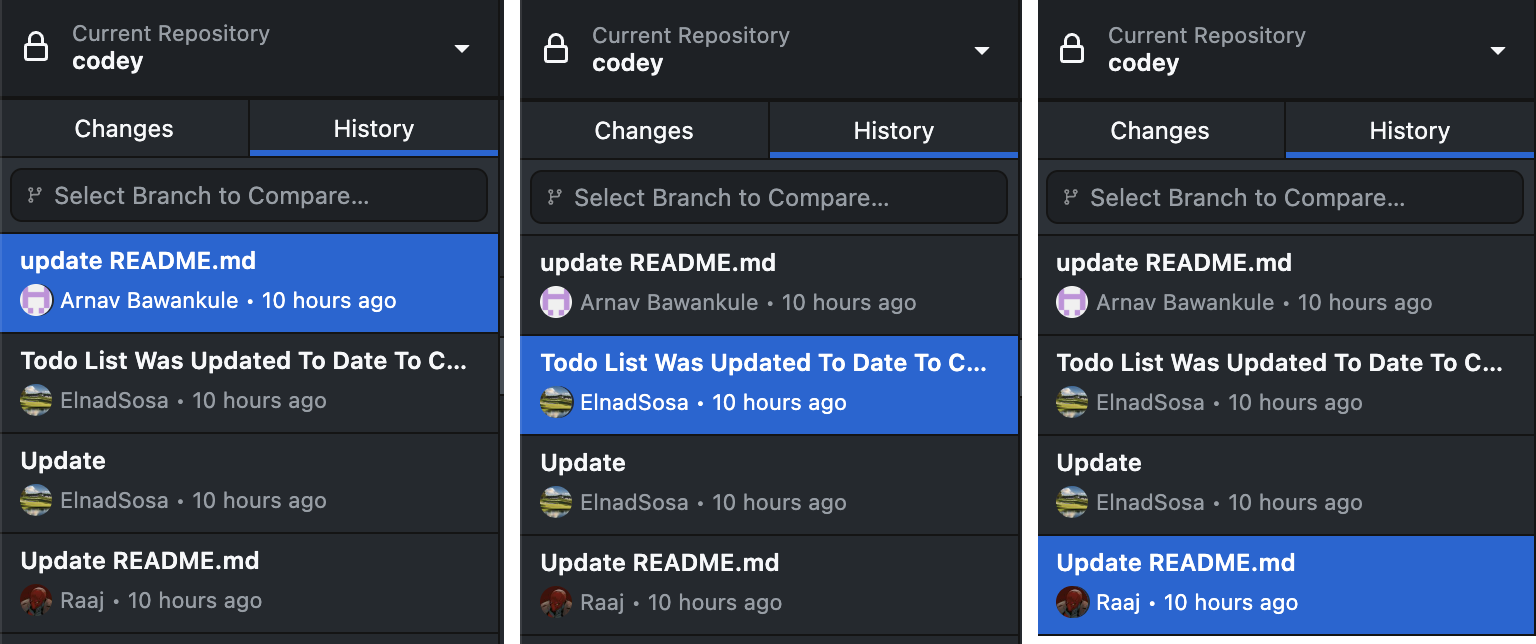
\includegraphics[width=\textwidth]{act81-history.png}
\caption{Activity 8.1: the History view on each member's machine after the pull, showing all three members' commits (original messages)}
\label{fig:act81history}
\end{figure}

\begin{table}[H]
\centering
\caption{Commits by author (\texttt{git shortlog -sn}, at the end of Sprint 4)}
\label{tab:shortlog}
\begin{tabularx}{\textwidth}{@{}L{4.2cm} l Y@{}}
\toprule
\textbf{Author} & \textbf{Commits} & \textbf{Notes} \\
\midrule
\multicolumn{3}{@{}l}{\tbd{run git shortlog -sn on main after the final merge}} \\
\bottomrule
\end{tabularx}
\end{table}

Most code was committed from one machine during pair-programming sessions, so the
commit counts understate the other members' share; the owner column of the Gantt
charts records who did each task. Since the November 5 history cleanup, commits carry
\texttt{Co-authored-by} trailers for the members who worked on them.

% =====================================================================
\section{Program Files and Configuration Files (Updated for Sprint 4)}\label{sec:files}
% =====================================================================
Table~\ref{tab:files} lists every file in the repository that the project uses:
Swift sources and tests, bundled data, build configuration, the database migrations,
scripts, the CI workflow, and the four documentation files that go with the code (the
READMEs, the design-system rules, and the pull request template), grouped by folder.
It is generated from \texttt{git ls-files} by \texttt{scripts/gen-file-table.py},
which stops if a file belongs to no group, so the table cannot silently miss a file.
Only the \texttt{docs/} folder (this document with its sources, figures, and
measurement data, the Sprint 2 document, and the course material), the project plan
(\texttt{todo.md}), and image assets (the app icon and the color sets generated by
\texttt{scripts/palette}) are not listed. Every listed file except
the documentation files has its own subsection in Appendix~B.

{\singlespacing\footnotesize
\IfFileExists{generated/file_table.tex}{% Generated by scripts/gen-file-table.py. Do not edit.
\begin{longtable}{@{}p{0.4\linewidth}p{0.08\linewidth}p{0.46\linewidth}@{}}
\caption{Program, configuration, and documentation files (376 files; all but the 5 Doc files are listed in Appendix~B)}\label{tab:files}\\
\toprule \textbf{Files} & \textbf{Type} & \textbf{Description} \\ \midrule
\endfirsthead
\toprule \textbf{Files} & \textbf{Type} & \textbf{Description} \\ \midrule
\endhead
\texttt{codey/Sources/CodeyApp.swift} & Source & App entry point: appearance and navigation-title setup, then LoadingView. \\
\texttt{codey/Sources/ContentView.swift} & Source & Root after boot: tab UI, onboarding cover, sync nudge when the app becomes active. \\
\texttt{codey/Sources/App/}: \texttt{AppAppearance.swift, AppConfig.swift, AppLaunchOptions.swift, LaunchTimer.swift, LoadingView.swift, Logging.swift} & Source & Boot sequence (store, seeding, badge catch-up), configuration from Info.plist, appearance preference, launch arguments, loggers, launch timer (NFR-01). \\
\texttt{codey/Sources/Models/Schema/}: \texttt{CodeyMigrationPlan.swift, CodeySchemaV1.swift, CodeySchemaV10.swift, CodeySchemaV11.swift, CodeySchemaV2.swift, CodeySchemaV3.swift, CodeySchemaV4.swift, CodeySchemaV5.swift, CodeySchemaV6.swift, CodeySchemaV7.swift, CodeySchemaV8.swift, CodeySchemaV9.swift} & Source & Versioned SwiftData schemas V1--V11 and the migration plan; shipped versions are never edited. \\
\texttt{codey/Sources/Models/Decks/}: \texttt{CardRating.swift, CodeLanguage.swift, CodeSnippet.swift, DeckOrigin.swift, Flashcard.swift, FlashcardDeck.swift} & Source & Deck and card models (FR-05--FR-08), code snippets, languages, ratings, deck origin. \\
\texttt{codey/Sources/Models/Progress/}: \texttt{BadgeAward.swift, DailyActivity.swift, QuestionProgress.swift, QuizAnswerRecord.swift, StudyProgressSnapshot.swift, TopicProgress.swift} & Source & Local progress models: question and topic progress, quiz answers, daily activity, study snapshots, badge awards (V7). \\
\texttt{codey/Sources/Models/Sync/}: \texttt{DeckSyncStateKind.swift, SyncOperation.swift} & Source & Persisted sync-state kind and queued sync operations. \\
\texttt{codey/Sources/Models/}: \texttt{ProfileAvatar.swift, Question.swift, Topic.swift, UserProfile.swift} & Source & Topics, questions and difficulty, user profile, avatar set (FR-04, FR-60). \\
\texttt{codey/Sources/ViewModels/}: \texttt{AskAISession.swift, CachedList.swift, DeckDraft.swift, DeckViewModel.swift, QuizViewModel.swift, StudySessionViewModel.swift} & Source & Observable view models for the deck builder, study sessions and quizzes, and the builder's draft types. \\
\texttt{codey/Sources/Services/Practice/}: \texttt{ChallengeLoader.swift, ChallengeRunner.swift, ExerciseLoader.swift, ExerciseValidator.swift, GatingConfig.swift, LeaderboardRanking.swift, QuestionPool.swift, QuizProgressStore.swift, SeededGenerator.swift, StudyPlanBuilder.swift, TierGate.swift} & Source & Adaptive practice: quiz builder, tier gates, gating thresholds, progress store, seeded RNG, weekly plan, leaderboard ranking; coding-exercise loader and validator (FR-39--FR-41). \\
\texttt{codey/Sources/Services/Gamification/}: \texttt{BadgeEvaluator.swift, LevelCalculator.swift, StreakCalculator.swift, WeeklyChallenge.swift, WeeklyXPStore.swift, XPPolicy.swift, XPRewards.swift} & Source & XP for answers, study, exercises and quest bonuses, levels, streaks and daily goal, badges, weekly challenge and weekly XP (FR-30--FR-35, FR-42, FR-43). \\
\texttt{codey/Sources/Services/Study/}: \texttt{StudyPool.swift, StudyQueue.swift} & Source & Study queue and study pool for flashcard sessions (FR-16--FR-18). \\
\texttt{codey/Sources/Services/Decks/}: \texttt{FlashcardFactory.swift, FlashcardPayload.swift, ModelValidator.swift, StableID.swift, StarterDeckLoader.swift} & Source & FlashcardFactory (Factory pattern), payloads, validator, starter-deck loader, stable IDs. \\
\texttt{codey/Sources/Services/Sync/}: \texttt{ConflictResolver.swift, DeckSyncState.swift, ProgressSync.swift, SyncCursorStore.swift, SyncEngine.swift, SyncQueue.swift} & Source & Sync engine, queue, cursors, conflict resolver, progress sync (FR-61), and the deck State pattern. \\
\texttt{codey/Sources/Services/AskAI/}: \texttt{AskAIPrompt.swift, OpenRouterClient.swift} & Source & Ask AI tutor: the only OpenRouter client, the system prompt, the chat session, and the answer-leak guard (FR-67, FR-68). \\
\texttt{codey/Sources/Services/Backend/Supabase/}: \texttt{KeychainSessionStorage.swift, SignInNonce.swift, SupabaseAuthProvider.swift, SupabaseDataClient+Content.swift, SupabaseDataClient.swift, SupabaseServices.swift, SupabaseTestClient.swift} & Source & The only folder that imports Supabase and GoogleSignIn: auth provider, data client, Keychain session storage, sign-in nonce, DEBUG stubbed-network test client. \\
\texttt{codey/Sources/Services/Backend/}: \texttt{AuthState.swift, BackendFacade+Decks.swift, BackendFacade+Groups.swift, BackendFacade+Profile.swift, BackendFacade.swift, BackendProtocols.swift, DeckBackend.swift, GroupCache.swift, NetworkMonitor.swift, SwiftDataService.swift} & Source & BackendFacade (Facade pattern) and its extensions, backend protocols, local store service, auth state, network monitor, group cache. \\
\texttt{codey/Sources/Services/Content/}: \texttt{ContentFiles.swift, ContentSeeder.swift} & Source & Content pipeline: ContentFiles (bundled, cached and downloaded content JSON) and ContentSeeder (validates a download and seeds it into the store). \\
\texttt{codey/Sources/Services/}: \texttt{BundledContentStamp.swift, DataSeeder.swift, LocalDataReset.swift, ModelContainerFactory.swift, QuestionBankLoader.swift} & Source & Model container factory, question-bank loader, data seeder, bundled-content stamp, local data reset. \\
\texttt{codey/Sources/DesignSystem/Tokens/}: \texttt{Colors.swift, Layout.swift, Motion.swift, Radius.swift, Spacing.swift, SyntaxRole.swift, TierStyle.swift, Typography.swift} & Source & Design tokens: colors, type, spacing, radius, motion, tier styles, syntax roles. \\
\texttt{codey/Sources/DesignSystem/Components/}: \texttt{AnswerOptionRow.swift, AppGlyph.swift, AskAIButton.swift, Bento.swift, CelebrationOverlay.swift, ChatBubble.swift, ChoiceChips.swift, CircleIconButton.swift, CloseButton.swift, CodeyButton.swift, CodeyCard.swift, CodeyChip.swift, CodeyOverlay.swift, CodeyPage.swift, EmptyStateView.swift, FlipCard.swift, FloatingPanel.swift, FormFeedback.swift, GameTiles.swift, HintBento.swift, Icon.swift, IconTable.swift, IconTile.swift, MasteryDots.swift, ProgressBar.swift, ProgressRing.swift, Session.swift, StatTile.swift, SwipeBack.swift, TierChipRow.swift, XPGainLabel.swift} & Source & Shared UI components built only from tokens. \\
\texttt{codey/Sources/DesignSystem/Markdown/}: \texttt{CardMarkdownComposition.swift, CardMarkdownView.swift, MarkdownFormatting.swift, MarkdownRichText.swift, MarkdownTextEditor.swift} & Source & Card Markdown rendering (the only Textual import) and the Markdown editor. \\
\texttt{codey/Sources/DesignSystem/CodeEditor/}: \texttt{CodeEditorView.swift, CodeyRunestoneTheme.swift} & Source & Runestone code editor and its theme (the only Runestone imports). \\
\texttt{codey/Sources/DesignSystem/Gallery/}: \texttt{ComponentGallery.swift} & Source & Component gallery previews (light, dark, large text). \\
\texttt{codey/Sources/Features/Home/}: \texttt{HomeComponents.swift, HomeLogic.swift, HomeView.swift} & Source & Play tab (the home dashboard): level, streak, quests, topic tiles with accuracy, and its pure logic (FR-36--FR-38, FR-53). \\
\texttt{codey/Sources/Features/Library/}: \texttt{LibraryView.swift} & Source & Library tab: every topic, and on each topic's page its quiz, coding exercises and decks. \\
\texttt{codey/Sources/Features/Decks/Builder/}: \texttt{BuilderSupport.swift, CardPageEditor.swift, CardPagerView.swift, DeckBuilderView.swift, DeckHeaderEditor.swift} & Source & Deck builder: header, card pager, card editor (UC-01, UC-02). \\
\texttt{codey/Sources/Features/Decks/}: \texttt{DeckDetailView.swift, DeckLibraryView.swift, DeckStatusChip.swift, DeckTile.swift} & Source & Deck library, deck detail, tiles, sync status chip (FR-48). \\
\texttt{codey/Sources/Features/Study/}: \texttt{CardRating+Display.swift, StudyCardView.swift, StudyLauncherSection.swift, StudySessionView.swift, StudySummaryView.swift} & Source & Study session screens: launcher, card, swipe rating, summary. \\
\texttt{codey/Sources/Features/Quiz/}: \texttt{ChallengeTiles.swift, ChallengeView.swift, ExerciseListView.swift, ExerciseView.swift, QuizModeView.swift, QuizRequest.swift, QuizSetupView.swift, QuizSummaryView.swift, QuizTopicStats.swift} & Source & Quiz setup panel, quiz run, summary, topic stats; coding-exercise tiles and exercise screen (FR-39--FR-41). \\
\texttt{codey/Sources/Features/AskAI/}: \texttt{AskAIChatView.swift} & Source & Ask AI chat panel and its button (FR-67). \\
\texttt{codey/Sources/Features/Profile/}: \texttt{BadgeViews.swift, FeedbackFormView.swift, ProfileEditorView.swift, ProfileSheet.swift} & Source & Profile sheet, profile editor, badges row, defect report form. \\
\texttt{codey/Sources/Features/Groups/}: \texttt{GroupBoardView.swift, GroupsView.swift} & Source & Groups list, create and join sheets, weekly leaderboard (FR-42, FR-50--FR-52). \\
\texttt{codey/Sources/Features/Onboarding/}: \texttt{OnboardingView.swift} & Source & Three-step first-launch onboarding. \\
\texttt{codey/Sources/Navigation/}: \texttt{RootView.swift, Router.swift, ViewModelHost.swift} & Source & Tab root and the router that owns tabs, sheets and covers. \\
\texttt{codey/Sources/Support/}: \texttt{Helpers.swift} & Source & Small generic helpers shared across features. \\
\texttt{codey/Tests/Performance/}: \texttt{PerfHarness.swift, PerformanceTests.swift} & Test & Performance suite TC-P01--TC-P07, the TC-P08 launch-store fixture, and the harness (opt-in, CODEY\_PERF=1). \\
\texttt{codey/Tests/}: \texttt{AppSettingsTests.swift, AskAITests.swift, BadgeEvaluatorTests.swift, BundledContentStampTests.swift, ChallengeTests.swift, ConflictResolverTests.swift, ContentFilesTests.swift, ContrastTests.swift, DataSeederTests.swift, DeckSyncStateTests.swift, DeckViewModelTests.swift, DesignSystemTests.swift, ExerciseLoaderTests.swift, ExercisePickerTests.swift, ExerciseValidatorTests.swift, FlashcardFactoryTests.swift, FlashcardMasteryTests.swift, FlashcardSchemaFileTests.swift, GoogleSignInLinkTests.swift, GroupsAndChallengeTests.swift, HomeLogicTests.swift, KeychainSessionStorageTests.swift, LevelCalculatorTests.swift, MarkdownRichTextTests.swift, MigrationTests.swift, ModelValidatorTests.swift, ProfileAndFeedbackTests.swift, ProgressHistorySyncTests.swift, ProgressSyncTests.swift, QuestionBankLoaderTests.swift, QuestionPoolTests.swift, QuestionProgressTests.swift, QuizViewModelTests.swift, SignInNonceTests.swift, StarterDeckLoaderTests.swift, StreakCalculatorTests.swift, StudyPlanBuilderTests.swift, StudyQueueTests.swift, StudySessionViewModelTests.swift, SupabaseDataClientTests.swift, SupabaseSchemaTests.swift, SyncEngineTests.swift, SyncQueueTests.swift, SyncTestSupport.swift, TestSupport.swift, TierGateTests.swift, XPPolicyTests.swift, XPRewardsTests.swift} & Test & Unit tests (Swift Testing) and shared fixtures and mocks. \\
\texttt{codey/UITests/}: \texttt{AccessibilityAuditUITests.swift, AskAIUITests.swift, DeckBuilderUITests.swift, ExerciseUITests.swift, ScreenTourUITests.swift, StudySessionUITests.swift, UITestNavigation.swift} & Test & XCTest UI tests: deck builder, study session, coding exercise, Ask AI (stubbed model), screen tour, accessibility audit. \\
\texttt{codey/Resources/Schemas/}: \texttt{flashcard.schema.json} & Resource & JSON Schema for a flashcard (FR-09); its limits match ModelValidator and SQL. \\
\texttt{codey/Resources/}: \texttt{challenges.json, exercises.json, questions-seed.json, starter-decks.json} & Resource & Bundled fallback copy of the content: question bank (8 topics, 176 questions), starter decks (12 decks, 144 cards), coding exercises (12). The source is the Supabase content\_* tables. \\
\texttt{Config/}: \texttt{Base.xcconfig, Secrets.example.xcconfig} & Config & Shared build settings and the secrets template; the real Secrets.xcconfig is gitignored. \\
\texttt{codey/codey.entitlements} & Config & Keychain access group, so Google sign-in keeps its session on Mac Catalyst. \\
\texttt{Project.swift} & Config & Tuist project: targets, Info.plist keys, dependencies. \\
\texttt{Tuist.swift} & Config & Tuist workspace configuration. \\
\texttt{Tuist/}: \texttt{Package.resolved, Package.swift} & Config & Swift package dependencies (pinned exact) and their resolved versions. \\
\texttt{.gitignore} & Config & Files kept out of Git (secrets, build output, backups). \\
\texttt{.mcp.json} & Config & Supabase MCP server for the project (used to run the live checks). \\
\texttt{supabase/migrations/}: \texttt{20261008022407\_profiles.sql, 20261008022417\_decks\_flashcards.sql, 20261008022422\_sync\_log.sql, 20261008022429\_rls.sql, 20261008022702\_lock\_down\_signup\_trigger.sql, 20261030200232\_avatar\_set\_feedback\_reports.sql, 20261030200303\_groups\_leaderboard.sql, 20261030200802\_s3\_advisor\_fixes.sql, 20261102182604\_weekly\_xp\_rate\_limit.sql, 20261110034534\_study\_progress.sql, 20261115045606\_avatar\_colors.sql, 20261115172929\_progress\_history.sql, 20261115194345\_card\_hidden.sql, 20261116002116\_content.sql, 20261117224554\_challenges.sql, 20261118035846\_more\_avatar\_colors.sql} & SQL & Database schema as ordered migrations: tables, CHECKs, RLS policies, groups, RPC, progress and history tables, public-read content\_* tables. \\
\texttt{supabase/seed.sql} & SQL & Content rows for the content\_* tables (8 topics, 192 questions, 25 exercises, 15 starter decks with 174 cards). \\
\texttt{supabase/challenges-seed.sql} & SQL & The 11 coding challenges with starters in four languages and every test, generated from supabase/content (S45). \\
\texttt{supabase/drill-hints.sql} & SQL & Two hints for each of the 55 drills (FR-74). \\
\texttt{supabase/functions/run-challenge/}: \texttt{drivers.ts, index.ts, judge.ts, judge\_test.ts} & Source & run-challenge Edge Function (Deno): limits, per-language test drivers, the judge, and its tests (FR-70, FR-71, NFR-33, NFR-34). \\
\texttt{supabase/content/challenges/binary-search/}: \texttt{challenge.json, solution.cpp, solution.java, solution.py, solution.swift, supabase/content/challenges/group-anagrams/challenge.json, supabase/content/challenges/group-anagrams/solution.cpp, supabase/content/challenges/group-anagrams/solution.java, supabase/content/challenges/group-anagrams/solution.py, supabase/content/challenges/group-anagrams/solution.swift, supabase/content/challenges/longest-substring/challenge.json, supabase/content/challenges/longest-substring/solution.cpp, supabase/content/challenges/longest-substring/solution.java, supabase/content/challenges/longest-substring/solution.py, supabase/content/challenges/longest-substring/solution.swift, supabase/content/challenges/max-subarray/challenge.json, supabase/content/challenges/max-subarray/solution.cpp, supabase/content/challenges/max-subarray/solution.java, supabase/content/challenges/max-subarray/solution.py, supabase/content/challenges/max-subarray/solution.swift, supabase/content/challenges/merge-intervals/challenge.json, supabase/content/challenges/merge-intervals/solution.cpp, supabase/content/challenges/merge-intervals/solution.java, supabase/content/challenges/merge-intervals/solution.py, supabase/content/challenges/merge-intervals/solution.swift, supabase/content/challenges/min-window/challenge.json, supabase/content/challenges/min-window/solution.cpp, supabase/content/challenges/min-window/solution.java, supabase/content/challenges/min-window/solution.py, supabase/content/challenges/min-window/solution.swift, supabase/content/challenges/order.json, supabase/content/challenges/product-except-self/challenge.json, supabase/content/challenges/product-except-self/solution.cpp, supabase/content/challenges/product-except-self/solution.java, supabase/content/challenges/product-except-self/solution.py, supabase/content/challenges/product-except-self/solution.swift, supabase/content/challenges/trapping-rain-water/challenge.json, supabase/content/challenges/trapping-rain-water/solution.cpp, supabase/content/challenges/trapping-rain-water/solution.java, supabase/content/challenges/trapping-rain-water/solution.py, supabase/content/challenges/trapping-rain-water/solution.swift, supabase/content/challenges/two-sum/challenge.json, supabase/content/challenges/two-sum/solution.cpp, supabase/content/challenges/two-sum/solution.java, supabase/content/challenges/two-sum/solution.py, supabase/content/challenges/two-sum/solution.swift, supabase/content/challenges/valid-palindrome/challenge.json, supabase/content/challenges/valid-palindrome/solution.cpp, supabase/content/challenges/valid-palindrome/solution.java, supabase/content/challenges/valid-palindrome/solution.py, supabase/content/challenges/valid-palindrome/solution.swift, supabase/content/challenges/valid-parentheses/challenge.json, supabase/content/challenges/valid-parentheses/solution.cpp, supabase/content/challenges/valid-parentheses/solution.java, supabase/content/challenges/valid-parentheses/solution.py, supabase/content/challenges/valid-parentheses/solution.swift, supabase/content/drill-hints.json} & Resource & Challenge sources: one folder per challenge with its JSON, tests and reference solutions in four languages, and the drill hints. \\
\texttt{supabase/tests/}: \texttt{challenges.sql, content.sql, history.sql, progress.sql, rls.sql} & SQL & pgTAP RLS and constraint tests (supabase test db). \\
\texttt{supabase/checks/}: \texttt{rls\_live\_check.sql} & SQL & The same checks for the live project (67 items, rolled back). \\
\texttt{supabase/config.toml} & Config & Supabase CLI settings for the local stack used by the pgTAP tests (seeding off). \\
\texttt{supabase/.gitignore} & Config & Keeps the Supabase CLI's local files out of Git. \\
\texttt{runner/}: \texttt{bootstrap.sh, configure-caddy.sh, push-secrets.sh, with-secrets.sh} & Script & Code-runner setup on EC2: Piston and Caddy bootstrap, secret creation, and moving the secrets to Supabase and GitHub without printing them. \\
\texttt{scripts/palette/}: \texttt{contrast.py, gen\_colors.py, palette.py, radix\_scales.json} & Script & Color palette, contrast checker, and asset-catalog generator (NFR-12). \\
\texttt{scripts/}: \texttt{backup.sh, challenges.ts, check-design-tokens.sh, check-imports.sh, check-release-build.sh, check-secrets.sh, gen-appendix-b.sh, gen-file-table.py, gen-pattern-map.sh, scripts/icons/icons.py, perf-launch.sh, perf-report.sh, render-app-icon.swift, test-report.py, test.sh} & Script & Repository checks, test runner and readable report, backups, icon rendering, performance runs, and the document generators. \\
\texttt{.github/workflows/}: \texttt{supabase-keepalive.yml, test.yml} & CI & GitHub Actions: tests and repository checks on every push to dev and main and every pull request to main (app, database, checks jobs); Supabase keep-alive every 3 days. \\
\texttt{README.md} & Doc & Repository overview, build summary, and the repository checks. \\
\texttt{codey/DESIGN\_SYSTEM.md} & Doc & Design-system rules: tokens, components, and what check-design-tokens.sh enforces. \\
\texttt{runner/SETUP.md} & Doc & Code-runner setup guide: EC2 instance, Elastic IP, budget alert, Piston, Caddy, secrets. \\
\texttt{supabase/README.md} & Doc & Supabase setup, migrations, RLS tests, operations, and the project's current state. \\
\texttt{.github/pull\_request\_template.md} & Doc & Merge checklist with the security items (Activity 10.1, SSC item 1). \\
\bottomrule
\end{longtable}
}{\tbd{run scripts/gen-file-table.py}}
}

% =====================================================================
\section{Project Security Issues (Updated for Sprint 4)}\label{sec:security}
% =====================================================================
Codey stores student progress on the phone and, for signed-in students, decks,
profiles, group memberships, weekly XP, and defect reports in Supabase. This section
summarizes the security requirements, the threat model (Activity~10.1), the design
principles applied, and the security tests re-run at the end of Sprint 4.

\subsection{Security Requirements}
The security non-functional requirements are NFR-04 to NFR-07 (encryption at rest on
the device and in the cloud, TLS 1.3 in transit, row ownership) and, added in
Sprint 3, NFR-21 to NFR-27 (Table~\ref{tab:nfr}): tokens only in the Keychain, no
secrets in the repository, server-side limits that mirror client validation, only the
two known hosts contacted, group data visible only to members, no test bypass in
Release builds, and a single exposed database function. Each names its verification
test, and Table~\ref{tab:sectests} records the results.

NFR-04 needs one clarification. The Activity~10.1 checklist listed a gap under item
13, because the store uses \emph{complete unless open} file protection while an
earlier version of NFR-04 asked for \emph{complete}. NFR-04 was amended in Sprint 2 to
\emph{complete unless open} on purpose (a sync in progress must be able to finish after
the device locks), so no gap remains; only the on-device check of the attribute is
outstanding (TC-S10, Table~\ref{tab:sectests}).

\subsection{Trust Boundary Analysis}
The critical trust boundary is between the iPhone app and the Supabase cloud (the
PostgREST API and PostgreSQL), crossed over the public internet. Everything on the
device side, including the app's own validation, must be assumed to be bypassable:
the public anon key ships inside the app and can be extracted to call the API
directly. Table~\ref{tab:boundary} records the main threat at this boundary and its
mitigations, updated for the Sprint 3 tables and function and the Sprint 4 progress tables.

\begin{table}[H]
\centering
\caption{Trust boundary: iPhone app $\to$ Supabase over the internet (Activity 10.1, updated)}
\label{tab:boundary}
\begin{tabularx}{\textwidth}{@{}Y Y@{}}
\toprule
\textbf{Threat: Broken Access Control (data tampering)} & \textbf{Mitigations} \\
\midrule
The extracted anon key is used to call the API directly. & Row Level Security on every table: a row is visible only to its owner (\texttt{owner\_id = auth.uid()}) or, for group data, to members of the same group. The anon role has no table access. \\
An attacker changes an \texttt{owner\_id}, \texttt{deck\_id}, or \texttt{group\_id} in a request to read, edit, or delete another user's data. & \texttt{owner\_id} and \texttt{created\_by} default to \texttt{auth.uid()} and are checked by RLS; group creation overwrites \texttt{created\_by} in a trigger; \texttt{join\_group} inserts a membership only for \texttt{auth.uid()}. \\
An attacker joins a group by guessing invite codes. & Codes are six characters from a 32-letter alphabet (about $1.1 \times 10^9$ codes), generated by the server. Each request tests one code, so guessing is impractical, and a correct guess grants only a seat on that group's weekly XP board. A server-side limit on join attempts is Sprint 4 hardening. \\
An attacker sends invalid or oversized data. & CHECK constraints mirror the app's limits (NFR-23); PostgREST sends parameterized queries, so SQL injection is not possible; the app never builds SQL. \\
A stolen session token is used to impersonate a user. & TLS 1.3 only; tokens only in the Keychain (\emph{after first unlock, this device only}) and never logged (NFR-21). \\
\bottomrule
\end{tabularx}
\end{table}

\subsection{Security Design Principles}
\begin{itemize}
  \item \textbf{Minimize the attack surface.} Only two external services (Supabase,
        Google). No custom server, open port, or admin screen. Database helper
        functions live in a \texttt{private} schema that PostgREST does not expose,
        and the sign-up trigger function and the dashboard's
        \texttt{rls\_auto\_enable()} are revoked from the API, so \texttt{join\_group}
        is the only callable function (NFR-27). It exists because joining needs to find
        a group the caller cannot see yet; it is \texttt{SECURITY DEFINER} with an
        empty \texttt{search\_path}, validates the code format, and can only insert
        the caller's own membership. Coding answers will be compared, not executed
        (R1). Supabase and Google imports are confined to one folder
        (\texttt{check-imports.sh}).
  \item \textbf{Least privilege.} The app uses only the anon and authenticated roles;
        the \texttt{service\_role} key is never in the app or the repository (NFR-22).
        Each user reads and writes only their own rows; group mates can read each
        other's display name, avatar, and weekly XP, nothing else. Defect reports are
        insert-only: users cannot read them back, not even their own. Google sign-in
        asks only for the basic profile and email scopes.
  \item \textbf{Defense in depth.} Input is checked in the app (\texttt{ModelValidator})
        and again by CHECK constraints; traffic is TLS 1.3; every request needs a valid
        session; RLS filters every row; data is encrypted at rest on the device (iOS
        file protection) and in the cloud (AES-256); and the secret scan and the pull
        request template's checklist run before each merge to \texttt{main}.
\end{itemize}

\subsection{Security Threat Model (Data Flow Diagram)}
Figure~\ref{fig:dfd} is the threat model as a data flow diagram: external entities
(rectangles), processes (circles), data stores (open rectangles), numbered data flows,
and trust boundaries (dashed red). Table~\ref{tab:stride} applies STRIDE to the flows
and elements that cross a boundary.

\begin{figure}[!htbp]
\centering
\resizebox{\textwidth}{!}{%
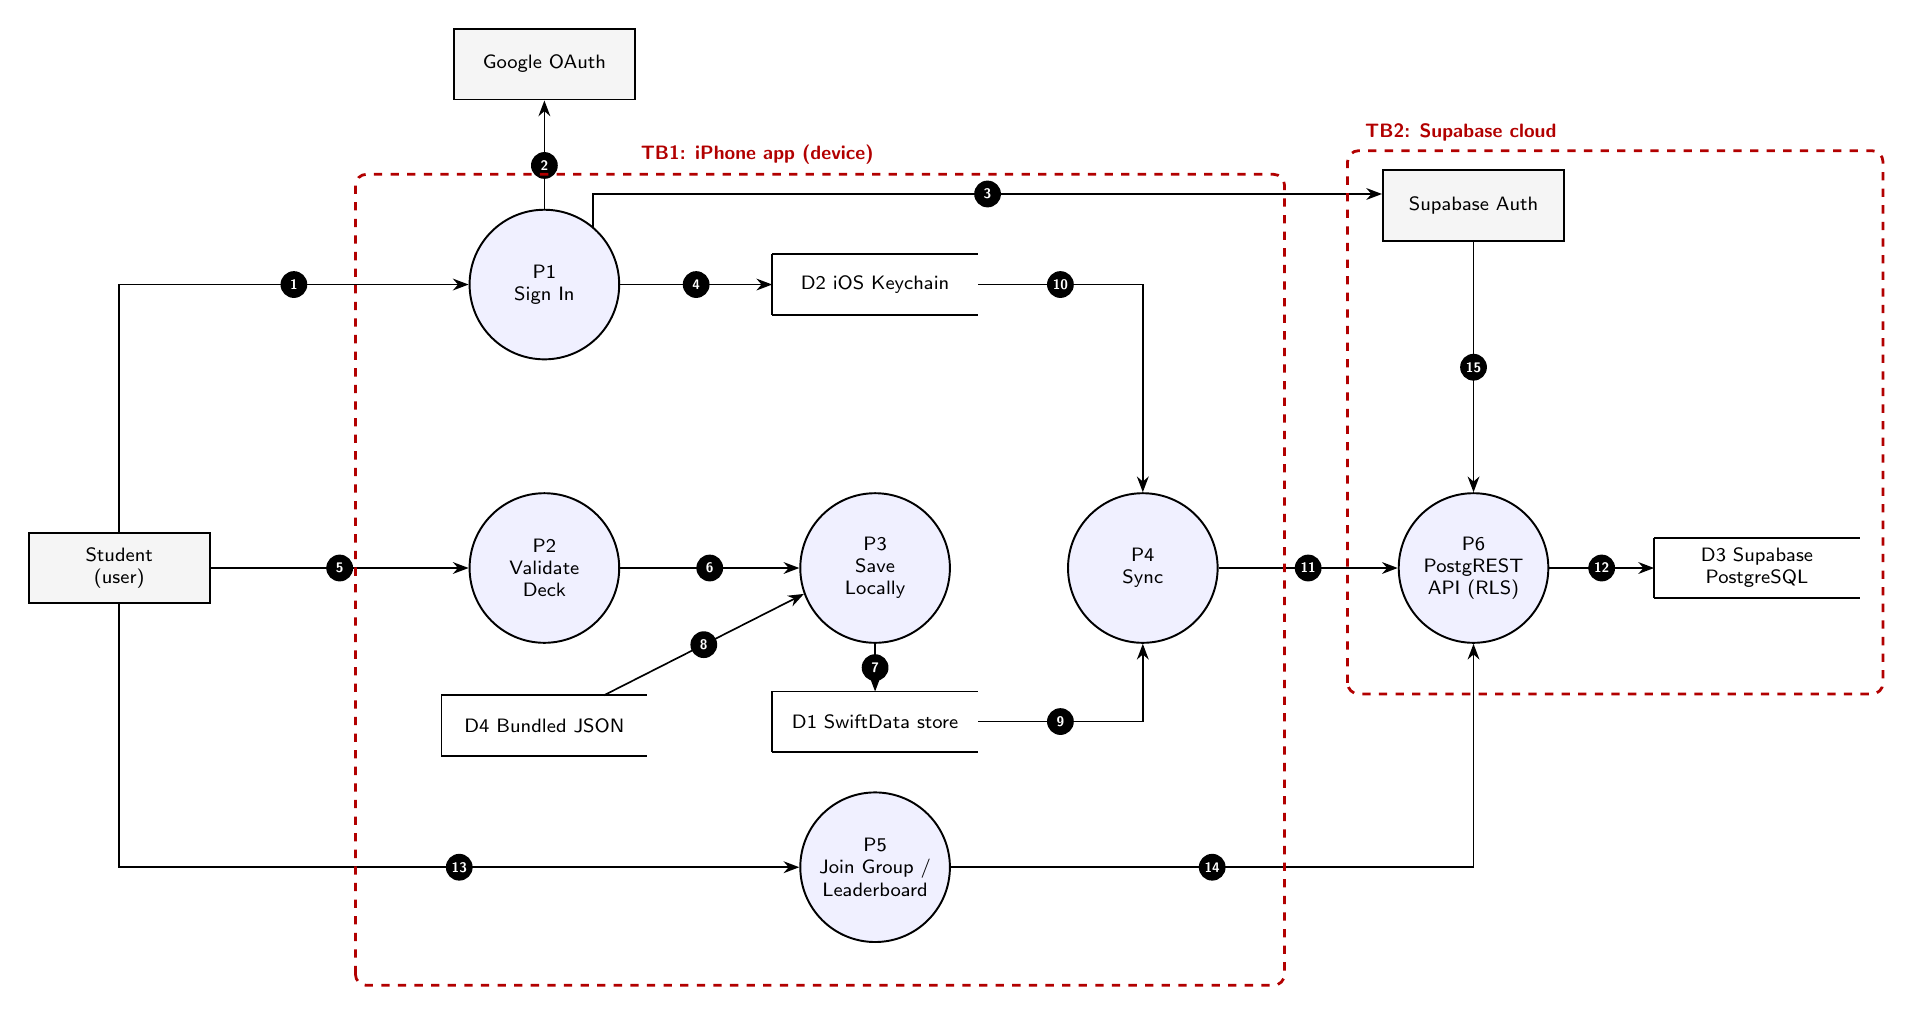
\begin{tikzpicture}[font=\sffamily\scriptsize,
    ent/.style={rectangle, draw, line width=0.7pt, fill=gray!8, minimum width=2.3cm, minimum height=0.9cm, align=center},
    proc/.style={circle, draw, line width=0.7pt, fill=blue!6, minimum size=1.9cm, align=center, inner sep=1pt},
    ds/.style={minimum width=2.6cm, minimum height=0.75cm, align=center, inner sep=2pt},
    fl/.style={line width=0.6pt, -{Stealth[length=2mm]}},
    fn/.style={circle, fill=black, text=white, inner sep=0.5pt, minimum size=3.4mm, font=\sffamily\tiny\bfseries},
    tb/.style={draw=red!70!black, dashed, line width=1pt, rounded corners=4pt}]
  % External entities
  \node[ent] (stu) at (-2.2,0) {Student\\(user)};
  \node[ent] (goo) at (3.2,6.4) {Google OAuth};
  \node[ent] (sau) at (15.0,4.6) {Supabase Auth};
  % Processes (device)
  \node[proc] (p1) at (3.2,3.6) {P1\\Sign In};
  \node[proc] (p2) at (3.2,0) {P2\\Validate\\Deck};
  \node[proc] (p3) at (7.4,0) {P3\\Save\\Locally};
  \node[proc] (p4) at (10.8,0) {P4\\Sync};
  \node[proc] (p5) at (7.4,-3.8) {P5\\Join Group /\\Leaderboard};
  % Processes (cloud)
  \node[proc] (p6) at (15.0,0) {P6\\PostgREST\\API (RLS)};
  % Data stores (open rectangles: top and bottom lines only)
  \node[ds] (d1) at (7.4,-1.95) {D1 SwiftData store};
  \node[ds] (d2) at (7.4,3.6) {D2 iOS Keychain};
  \node[ds] (d4) at (3.2,-2.0) {D4 Bundled JSON};
  \node[ds] (d3) at (18.6,0) {D3 Supabase\\PostgreSQL};
  \foreach \d in {d1,d2,d3,d4}{
    \draw[line width=0.7pt] (\d.north west) -- (\d.north east);
    \draw[line width=0.7pt] (\d.south west) -- (\d.south east);
    \draw[line width=0.7pt] (\d.north west) -- (\d.south west);}
  % Flows
  \draw[fl] (stu) |- node[fn, pos=0.75] {1} (p1);
  \draw[fl] (p1) -- node[fn, pos=0.4] {2} (goo);
  \draw[fl] (p1.50) |- node[fn, pos=0.75] {3} (sau.west |- 0,4.75);
  \draw[fl] (p1) -- node[fn] {4} (d2);
  \draw[fl] (stu) -- node[fn] {5} (p2);
  \draw[fl] (p2) -- node[fn] {6} (p3);
  \draw[fl] (p3) -- node[fn] {7} (d1);
  \draw[fl] (d4) -- node[fn] {8} (p3.200);
  \draw[fl] (d1) -| node[fn, pos=0.25] {9} (p4);
  \draw[fl] (d2) -| node[fn, pos=0.25] {10} (p4);
  \draw[fl] (p4) -- node[fn] {11} (p6);
  \draw[fl] (p6) -- node[fn] {12} (d3);
  \draw[fl] (stu) |- node[fn, pos=0.75] {13} (p5);
  \draw[fl] (p5) -| node[fn, pos=0.25] {14} (p6);
  \draw[fl] (sau) -- node[fn] {15} (p6);
  % Trust boundaries
  \draw[tb] (0.8,-5.3) rectangle (12.6,5.0);
  \node[anchor=south west, text=red!70!black, font=\sffamily\scriptsize\bfseries] at (4.3,5.0) {TB1: iPhone app (device)};
  \draw[tb] (13.4,-1.6) rectangle (20.2,5.3);
  \node[anchor=south west, text=red!70!black, font=\sffamily\scriptsize\bfseries] at (13.5,5.3) {TB2: Supabase cloud};
\end{tikzpicture}}
\caption{Security threat model as a data flow diagram (external entities, processes P1--P6, data stores D1--D4, numbered flows, trust boundaries TB1 and TB2)}
\label{fig:dfd}
\end{figure}

The numbered flows are: (1) the student starts sign-in; (2) the Google sign-in sheet
returns an ID token; (3) the token is exchanged with Supabase Auth for a session; (4)
the session is stored in the Keychain; (5) the student types deck text and code; (6)
the validated draft is passed on; (7) decks and progress are written to the store; (8)
bundled starter decks and questions are seeded; (9) queued changes and (10) the access
token are read by the sync engine; (11) batched upserts and pulls go to PostgREST over
HTTPS; (12) PostgREST queries PostgreSQL under the caller's RLS policies; (13) the
student enters an invite code or opens a board; (14) \texttt{join\_group} and the
leaderboard view are called; (15) PostgREST verifies the session's JWT issued by
Supabase Auth.

\begin{xltabular}{\textwidth}{@{}L{2.1cm} L{2.4cm} Y Y@{}}
\caption{STRIDE analysis of the threat model}\label{tab:stride}\\
\toprule
\textbf{Element / flow} & \textbf{STRIDE threat} & \textbf{Scenario} & \textbf{Mitigation} \\
\midrule
\endfirsthead
\multicolumn{4}{@{}l}{\small\itshape Table \thetable\ continued} \\
\toprule
\textbf{Element / flow} & \textbf{STRIDE threat} & \textbf{Scenario} & \textbf{Mitigation} \\
\midrule
\endhead
\bottomrule
\endfoot
Flows 2, 3, 15 & Spoofing & A forged ID token or session is presented. & Supabase Auth verifies Google's token signature; PostgREST verifies the JWT on every request. \\
Flows 11, 14 & Tampering, Information disclosure & A network attacker reads or alters traffic (public Wi-Fi). & TLS 1.3 minimum, no ATS exceptions (NFR-06); traffic capture TC-S09. \\
P6 / D3 & Elevation of privilege, Information disclosure & A user reads or writes another user's rows, or a non-member reads a group board. & RLS on all 11 tables; group policies via \texttt{private.is\_member()}; 48 live checks, 0 failures (TC-S01). \\
Flow 14 & Elevation of privilege & \texttt{join\_group} (definer rights) is abused to add another user or read other groups. & Inserts only \texttt{auth.uid()}; empty \texttt{search\_path}; returns only the joined group; revoked from anon. \\
D3 (\texttt{weekly\_xp}) & Tampering & A user writes an inflated weekly XP. & Own row only, CHECK $\le$ 22,500, server keeps the maximum, growth clamped to 600 XP per minute; accepted residual risk R13. \\
D2, flow 10 & Information disclosure & The session token leaks from storage or logs. & Keychain, this device only; logging audit: the 7 public log values are a launch duration, starter-deck keys and card IDs, sync event, state, and entity names, and tier names (NFR-21). \\
D1 & Information disclosure & A lost phone exposes progress and decks. & iOS Data Protection (\emph{complete unless open}). The offline group cache (group names, invite codes, member names) is in \texttt{UserDefaults}, which has the default protection, and is cleared on sign-out. \\
P2, flow 5 & Tampering, Denial of service & Oversized or malformed input crashes the app or the server. & Validator limits (title 60, text 500, code 2,000 characters and 80 lines), errors as values; CHECK constraints server-side. \\
Flow 11 & Repudiation & A user denies having pushed a change. & Append-only \texttt{sync\_log} with no update or delete policies. \\
P6 & Denial of service & Request flooding exhausts the Free plan. & Every write needs a signed-in session and passes RLS and CHECK constraints; usage is reviewed monthly against the Free-plan limits (NFR-20, R11). Weekly XP writes are pace-limited by a trigger (at most 600 XP per minute of server time, clamped rather than rejected; migration \texttt{weekly\_xp\_rate\_limit}). Other tables have no per-user rate limit, accepted for a class-sized user base (R11). \\
\end{xltabular}

\subsection{Security Test Cases}
Table~\ref{tab:sectests} lists the security test cases, built from the automated
checks of Activity~10.1, with the result of the Sprint 4 run. Activity~10.1 chose
tool-based analysis: each check is an automated, repeatable tool run, so results can
be compared sprint to sprint (NFR-18). The checks run on every change that touches
the backend and in full at the end of each sprint, and a failed check blocks the merge
to \texttt{main} until it is fixed and run again. Since Sprint 4, TC-S03, TC-S05,
TC-S11, TC-S12 and the unit tests behind TC-S06 and TC-S08 run in GitHub Actions on
every push to \texttt{main} and \texttt{dev} (Section~\ref{sec:vc}). TC-S01 and TC-S02
need the live project and are run by hand after each migration; TC-S09 and TC-S10
need Proxyman and a physical iPhone.

\begin{xltabular}{\textwidth}{@{}L{1.2cm} L{2.4cm} Y L{2.4cm} L{2.4cm} L{1.5cm}@{}}
\caption{Security test cases and Sprint 4 results}\label{tab:sectests}\\
\toprule
\textbf{ID} & \textbf{Item} & \textbf{Steps} & \textbf{Expected} & \textbf{Actual (date)} & \textbf{Status} \\
\midrule
\endfirsthead
\multicolumn{6}{@{}l}{\small\itshape Table \thetable\ continued} \\
\toprule
\textbf{ID} & \textbf{Item} & \textbf{Steps} & \textbf{Expected} & \textbf{Actual (date)} & \textbf{Status} \\
\midrule
\endhead
\bottomrule
\endfoot
TC-S01 & Row Level Security, live (NFR-07, NFR-25) & Run \texttt{supabase/checks/rls\_live\_check.sql} in the Supabase SQL editor (or through the Supabase MCP server); two simulated users and a non-member try to read, change, and delete each other's rows on all 11 tables; everything rolls back. & 0 of 57 checks fail & 0 of 57 failed (Nov 9) & Pass \\
TC-S02 & Security Advisor (NFR-27) & Run the Supabase Security Advisor after each migration; fix or justify each warning. & 0 unjustified warnings & 1 fixed (\texttt{rls\_auto\_enable}); 1 justified (\texttt{join\_group}) (Oct 30); \tbd{re-run after the progress migration} & \tbd{status} \\
TC-S03 & Secret scan (NFR-22) & \texttt{scripts/check-secrets.sh -{}-history}: key-shaped strings in tracked files and every commit, plus the real values from the local \texttt{Secrets.xcconfig}. & 0 findings & 0 key-shaped strings, 0 real values (CI, Nov 14) & Pass \\
TC-S04 & Static analysis & \texttt{xcodebuild analyze -scheme codey}; count security warnings. & 0 & 0 security findings; 22 warnings, all in third-party packages, 0 in Codey's sources (Nov 14) & Pass \\
TC-S05 & No test bypass in Release (NFR-26, SSC 12) & \texttt{scripts/check-release-build.sh}: build Release, search the binary's symbols and strings for the DEBUG-only names. & None found & None found (CI, Nov 14) & Pass \\
TC-S06 & Server limits match client (NFR-23) & \texttt{SupabaseSchemaTests}, \texttt{FlashcardSchemaFileTests}. & Pass & Pass in the 402-test run (Nov 14) & Pass \\
TC-S07 & Token storage and logging (NFR-21) & \texttt{KeychainSessionStorageTests}; search the source for public log values and \texttt{UserDefaults} writes of tokens. & Keychain only; no token logged & 7 public log values, none sensitive; no token in \texttt{UserDefaults} (Oct 30) & Pass \\
TC-S08 & TLS 1.3, no ATS exceptions (NFR-06) & \texttt{TransportSecurityTests}, \texttt{AppConfigTests} (Info.plist). & Pass & Pass in the 402-test run (Nov 14) & Pass \\
TC-S09 & Hosts and TLS on the wire (NFR-24) & Capture Simulator traffic with Proxyman during sign-in, sync, and a leaderboard load. & Only Supabase and Google, all TLS 1.3 & \tbd{result and date} & \tbd{status} \\
TC-S10 & File protection on device (NFR-04) & Install on an iPhone, read the store files' protection attribute. & \emph{complete unless open} & \tbd{result and date} & \tbd{status} \\
TC-S11 & SDK confinement (R7) & \texttt{scripts/check-imports.sh}. & Pass & Pass (CI, Nov 14) & Pass \\
TC-S12 & Database policies and triggers (NFR-07, NFR-25, FR-61) & \texttt{supabase test db}: pgTAP suites \texttt{rls.sql} and \texttt{progress.sql} against a fresh local database built from the 10 migrations. & 75 of 75 pass & 75 of 75 passed (CI, Nov 14) & Pass \\
\end{xltabular}

\subsection{Software Security Checklist}
Table~\ref{tab:ssc} is the project's security checklist from Activity~10.1 (items 1--5
and 21 of the course table, plus items 12, 13, 18, and 22), with the result at the end
of Sprint 4.

\begin{xltabular}{\textwidth}{@{}l L{2.5cm} Y L{4.2cm}@{}}
\caption{Software security checklist with Sprint 4 results}\label{tab:ssc}\\
\toprule
\textbf{\#} & \textbf{Item} & \textbf{Team approach} & \textbf{Actual result (Sprint 4)} \\
\midrule
\endfirsthead
\multicolumn{4}{@{}l}{\small\itshape Table \thetable\ continued} \\
\toprule
\textbf{\#} & \textbf{Item} & \textbf{Team approach} & \textbf{Actual result (Sprint 4)} \\
\midrule
\endhead
\bottomrule
\endfoot
1 & Security review in every phase & Security items in the PR template, checked before each merge to \texttt{main}; security walkthrough at each sprint review. & In use since Sprint 2; the Sprint 4 progress migration was checked against it before it was applied (Nov 9), and CI now runs the automated checks on every push. \\
2 & Security metrics and trace matrix & Security metrics compared sprint to sprint; security NFRs traced to test cases. & Sprint 3 vs Sprint 4 values in Table~\ref{tab:metrics}; NFR-21--27 traced to TC-S01--S12. \\
3 & Stakeholders and their security needs & Students: private, encrypted progress; client: no cost, team-written code; team: no leaked keys. & Complete; group mates see only name, avatar, and weekly XP. \\
4 & Usage context and operating environment & iPhone app, offline-capable, Supabase Free plan over the public internet, possibly public Wi-Fi. & Complete; NFR-03 to NFR-06. \\
5 & Language and OS risks shared before design & Swift is memory-safe; known risks: secrets in logs, ATS exceptions, tokens in \texttt{UserDefaults}, RLS off by default. & Complete; documented in \texttt{supabase/README.md}, the PR template, and the secrets template. \\
21 & Data from app server to database & RLS on every table; server-assigned owner; CHECK constraints; parameterized queries; SSL to Postgres; AES-256 at rest. & RLS on 11 of 11 tables; 57 live checks, 0 failed; 75 pgTAP tests pass in CI. \\
12 & No backdoors or bypass paths & Test sign-in compiled only in DEBUG; no admin screens; internal functions revoked from the API. & DEBUG guard in place; Release check finds none of the DEBUG-only names on every CI run (TC-S05). \\
13 & No secrets in code; no weak encryption & Keys only in the gitignored \texttt{Secrets.xcconfig}; secret scan; Keychain; Apple and Supabase encryption, no custom crypto. & Pattern scan 0 findings. The Sprint 2 ``gap'' is closed: NFR-04 was amended to \emph{complete unless open}. \\
18 & Secure connections & TLS 1.3 minimum in code; no ATS exceptions; traffic capture. & Code and tests pass; capture \tbd{TC-S09 result}. \\
22 & No default or improper configuration & RLS on every table; anon has no table access; Security Advisor each sprint; Google OAuth in Testing mode. & Advisor: 1 warning fixed, 1 justified (Oct 30); \tbd{re-run}. \\
\end{xltabular}

% =====================================================================
\section{System Performance (Updated for Sprint 4)}\label{sec:performance}
% =====================================================================
This section defines the performance requirements, the test cases and profiles that
measure them, the results, and the bottlenecks. Every number states how it was
measured. Following Activity~9.2, each scenario runs 10 times in a row; the first run
is discarded as a warm-up, and the mean, 95th percentile (p95), and standard deviation
of the other nine are reported. With nine samples the nearest-rank p95 is the slowest
kept run, which makes it a conservative bound.

\subsection{Performance Requirements}
Table~\ref{tab:perfreq} collects the performance requirements. NFR-01 and NFR-02 come
from the client's mandatory list and Activity~9.2; NFR-28 to NFR-32 were added in
Sprint 3 for the paths a student waits on. NFR-32 (leaderboard load) was retired in Sprint 4
(decision S33): it needed live test accounts, which were dropped. The thresholds are not arbitrary: each is
set from what the student experiences (a quiz or a save should feel instant, under
the roughly 100 ms at which a delay becomes noticeable), and each was checked against a
first baseline run before it was published.

\begin{table}[H]
\centering
\caption{Performance requirements}
\label{tab:perfreq}
\begin{tabularx}{\textwidth}{@{}l Y L{2.0cm} L{3.0cm}@{}}
\toprule
\textbf{ID} & \textbf{Requirement} & \textbf{Threshold} & \textbf{Test case} \\
\midrule
NFR-01 & Home dashboard ready after a cold launch & $\le$ 3 s (p95) & TC-P08 \\
NFR-02 & 100-card deck pushed to Supabase on Wi-Fi & $\le$ 5 s & TC-P07 (mock) \\
NFR-28 & Peak memory footprint, 100-card study session & $\le$ 150 MB & TC-P03 \\
NFR-29 & Build a 10-question quiz & $\le$ 50 ms (p95) & TC-P01 \\
NFR-30 & Validate and save a 100-card deck locally & $\le$ 250 ms (p95) & TC-P02 \\
NFR-31 & First render of a card with an 80-line snippet & $\le$ 100 ms (p95) & TC-P06 \\
\bottomrule
\end{tabularx}
\end{table}

\subsection{Performance Test Cases}
The test data follows Activity~9.2: the full bundled content (8 topics, 176 questions,
12 starter decks with 144 cards) plus generated user decks built through the real
\texttt{FlashcardFactory} and validator. A generated deck has 100 cards with Markdown
prompts and answers; every third card carries a 12-line Swift snippet, and tiers
rotate Easy, Medium, Hard. The suite is \texttt{codey/Tests/Performance}; it is
skipped in normal test runs and enabled with \texttt{CODEY\_PERF=1}, and
\texttt{scripts/perf-report.sh} runs it and writes the results to
\texttt{docs/source/perf/<tag>.csv} (\texttt{PERF\_TAG}, default \texttt{sprint4}), so
each sprint's results stay next to the earlier ones.

\textbf{Testing approach (Activity 9.2).} The team chose a hybrid approach. Internal
resources run inside the app or its test host: the XCTest-hosted
\texttt{PerformanceTests} with in-process timers and \texttt{task\_info}, the app's
own \texttt{LaunchTimer}, and Instruments for diagnosis. External resources observe
from outside: \texttt{perf-launch.sh} relaunches the app with \texttt{simctl} and
reads its log. Network Link Conditioner and the Supabase dashboard logs, also planned
in Activity~9.2, were for live network tests; those were dropped with the test
accounts (S33), so the network profile is measured against a mock with a fixed
latency. Every run used the iOS Simulator (Table~\ref{tab:hardware}); the device
checks are listed separately.

\begin{xltabular}{\textwidth}{@{}L{1.3cm} L{2.6cm} Y L{2.3cm} L{1.9cm}@{}}
\caption{Performance test cases}\label{tab:perftests}\\
\toprule
\textbf{ID} & \textbf{Scenario (test)} & \textbf{Input and steps} & \textbf{Metric} & \textbf{Expected} \\
\midrule
\endfirsthead
\multicolumn{5}{@{}l}{\small\itshape Table \thetable\ continued} \\
\toprule
\textbf{ID} & \textbf{Scenario (test)} & \textbf{Input and steps} & \textbf{Metric} & \textbf{Expected} \\
\midrule
\endhead
\bottomrule
\endfoot
TC-P01 & Quiz build (\texttt{quizBuild}) & Seeded store; create a mixed 10-question \texttt{QuizViewModel} for the first topic with a new seed each run (fetches + \texttt{QuestionPool.build}). & Time & p95 $\le$ 50 ms \\
TC-P02 & Deck save (\texttt{deckSave100Cards}) & Fresh in-memory store per run; \texttt{BackendFacade.saveDeck} of the 100-card draft (validate, factory, insert, queue 101 operations, save). & Time & p95 $\le$ 250 ms \\
TC-P03 & Study session (\texttt{studySession100CardsMemory}) & Seeded store with a saved 100-card deck; reveal and rate Easy until the session finishes. & Peak footprint; time & $\le$ 150 MB \\
TC-P04 & Question-bank seeding (\texttt{dataSeederCold}) & Empty store; decode \texttt{questions-seed.json} (83 KB) and upsert 8 topics and 176 questions. & Time & Informational \\
TC-P05 & Starter-deck seeding (\texttt{starterDeckSeed}) & Store with topics; decode \texttt{starter-decks.json} (66 KB) and create 144 cards through the factory. & Time & Informational \\
TC-P06 & Snippet render (\texttt{highlight80LineSnippet}) & Render a card with an 80-line Swift snippet off-screen (\texttt{ImageRenderer}, 390 pt wide): Markdown parse, Prism highlighting, layout. & Time & p95 $\le$ 100 ms \\
TC-P07 & Sync push (\texttt{syncPush100CardsMockRTT}) & Signed-in facade on a mock backend that waits 50 ms per request; save a 100-card deck, then one full sync cycle. & Time & $\le$ 5 s \\
TC-P08 & Cold launch (\texttt{perf-launch.sh}) & App installed on the booted Simulator, onboarding done, store with the starter decks and 5 user decks of 50 cards; terminate and relaunch 10 times; read \texttt{home-ready} from the log. & Time & p95 $\le$ 3 s \\
\end{xltabular}

\subsection{Performance Profile Definitions}
A profile is one user-facing path with the resources it is measured on:
\begin{itemize}
  \item \textbf{Launch profile} (TC-P04, TC-P05, TC-P08): process start to Home's first
        appearance, which includes opening the store, seeding bundled content, and the
        first SwiftData queries on Home. Measured: wall time.
  \item \textbf{Study profile} (TC-P03, TC-P06): a long study session and the most
        expensive card to draw. Measured: peak physical footprint (the value Xcode's
        memory gauge shows, read with \texttt{task\_info}), wall time.
  \item \textbf{Practice profile} (TC-P01): starting a quiz. Measured: wall time.
  \item \textbf{Authoring profile} (TC-P02): saving a large deck. Measured: wall time
        on the main actor, where the save runs.
  \item \textbf{Network profile} (TC-P07): pushing
        and pulling changes. Measured: wall time and the number of requests.
\end{itemize}
Measurements were taken on the iOS Simulator on the machine recorded in
Table~\ref{tab:hardware}, with the Release configuration (testability enabled) on an
iPhone 17 Simulator, iOS 27.0 runtime (24A5370g), on Nov 14, 2026 at commit
\texttt{535911e} (\texttt{perf/sprint4-environment.txt}). The Sprint 3 run (Oct 31,
\texttt{e12c8b6}) used the same Mac, Xcode, and runtime on macOS 27.2; its files are
kept for the comparison in Table~\ref{tab:perfcompare}.

\subsection{Results}
\IfFileExists{perf/sprint4.csv}{%
Table~\ref{tab:perfresults} and Figure~\ref{fig:perfchart} report the results.

\begin{table}[H]
\centering
\caption{Performance results (9 kept runs per scenario; times in ms). Peak MB is the whole test process on the Simulator, about 200~MB of which is iOS framework pages (Section~\ref{sec:bottlenecks}); Growth MB is the most one run of the scenario added to it.}
\label{tab:perfresults}
\resizebox{\textwidth}{!}{%
\pgfplotstabletypeset[col sep=comma, string type,
  create on use/tc/.style={create col/set list={TC-P02,TC-P06,TC-P01,TC-P04,TC-P05,TC-P03,TC-P07}},
  columns={tc,name,mean_ms,p95_ms,stddev_ms,peak_mb,growth_mb,threshold_ms},
  columns/tc/.style={column name=TC},
  every head row/.style={before row=\toprule, after row=\midrule},
  every last row/.style={after row=\bottomrule},
  columns/name/.style={column name=Scenario},
  columns/runs/.style={column name=Runs},
  columns/mean_ms/.style={column name=Mean},
  columns/p95_ms/.style={column name=p95},
  columns/stddev_ms/.style={column name=Std.\ dev.},
  columns/peak_mb/.style={column name=Peak MB},
  columns/growth_mb/.style={column name=Growth MB},
  columns/threshold_ms/.style={column name=Threshold}]{perf/sprint4.csv}}
\end{table}

\begin{figure}[!htbp]
\centering
\begin{tikzpicture}
\pgfplotstableread[col sep=comma]{perf/sprint4.csv}\perftable
\begin{axis}[xbar, xmode=log, log origin=infty, width=0.72\textwidth, height=8cm,
    xlabel={Time (ms, log scale)}, ylabel={Scenario},
    ytick={0,...,6}, yticklabels from table={\perftable}{name},
    yticklabel style={font=\scriptsize},
    enlarge y limits=0.08, legend style={at={(0.98,0.02)}, anchor=south east, font=\scriptsize}]
  \addplot table[x=mean_ms, y expr=\coordindex] {\perftable};
  \addplot table[x=p95_ms, y expr=\coordindex] {\perftable};
  \legend{Mean, p95}
\end{axis}
\end{tikzpicture}
\caption{Mean and p95 time per scenario. X-axis: time in milliseconds, log scale; Y-axis: scenario. The TC-P08 launch (4.23~s at p95) is reported in the text.}
\label{fig:perfchart}
\end{figure}
}{\tbd{run scripts/perf-report.sh and scripts/perf-launch.sh; the table and chart are
built from docs/source/perf/sprint4.csv}}

Against each requirement (p95 over 9 kept runs):
\begin{itemize}
  \item \textbf{NFR-01, launch (TC-P08): not met on the Simulator.} Home was ready
        4.23~s after process start (mean 4.20~s, standard deviation 22.5~ms,
        \texttt{docs/source/perf/sprint4-launch.csv}) against
        3~s, with the TC-P08 store (the starter decks plus five 50-card user decks,
        written by the \texttt{LaunchFixtureSeed} test before timing). An Instruments App Launch trace and the
        dynamic loader's log show where the time goes: about 3.3~s pass in the
        Simulator's loader (\texttt{dyld\_sim}) before any Codey code runs, loading
        about 1{,}600 iOS system images (counted with \texttt{DYLD\_PRINT\_LIBRARIES}).
        Codey's own work, from \texttt{main} to Home's first appearance, is about
        0.6~s: down from 1.0~s after the loading screen's 0.4~s minimum was
        removed and boot began skipping the starter-content reseed when the bundled
        content is unchanged (a SHA-256 stamp, \texttt{BundledContentStamp}).
        Sprint~4 is 0.41~s slower than Sprint~3 (3.82~s). A probe that logged the
        time at \texttt{main} split the Sprint~4 launch into 3.56~s before Codey's
        code and 0.62~s after it (means of 9 runs), so the app's own share did not
        change; the time before \texttt{main} grew by about 0.26~s. Of that,
        about 60~ms is the \texttt{-ObjC} linker flag added for BUG-01, which loads
        every Objective-C class of the statically linked packages (measured by
        launching a build without it: 4.17~s); the rest coincides with the macOS
        27.2.1 update of the Mac that hosts the Simulator. For scale,
        a one-view SwiftUI app reached its first view in 1.2--1.9~s on the same
        Simulator. On an iPhone those system images come from the shared cache, so
        the Simulator figure overstates launch; the requirement stays open until it
        is measured on a device: \tbd{iPhone cold-launch p95 and date}.
  \item \textbf{NFR-02, 100-card sync (TC-P07): met against the mock backend.} 0.42~s
        against 5~s, with 50~ms of latency per request; not measured live (S33).
  \item \textbf{NFR-28, memory (TC-P03): not met on the Simulator.} The whole test
        process peaked at 282.9~MB against 150~MB, while a full 100-card session
        added at most 1.5~MB to the footprint. About 205~MB of an idle Codey process on the
        Simulator is iOS framework data (\texttt{\_\_DATA\_CONST}, \texttt{\_\_DATA}, and
        mapped files) that a device keeps in the shared cache; the heap was about
        31~MB. So the session itself is cheap, but the requirement names the peak
        footprint, so it stays open until it is measured on the iPhone 16 Pro Max:
        \tbd{device peak footprint and date}. The test gates on the session's growth, which it can control on the
        Simulator, and reports both numbers.
  \item \textbf{NFR-29, quiz build (TC-P01): met.} 0.37~ms against 50~ms.
  \item \textbf{NFR-30, deck save (TC-P02): met.} 38.7~ms against 250~ms, a third
        faster than in Sprint~3 (57.9~ms): the Nov~2 refactor (\texttt{d549198}) replaced
        one store fetch per changed card (100 for this deck) with a lookup in the
        deck's own cards when the save queues them for sync.
  \item \textbf{NFR-31, 80-line render (TC-P06): met.} 13.8~ms against 100~ms.
\end{itemize}

Table~\ref{tab:perfcompare} compares the two sprints (p95, same Mac, Simulator, and
runtime). Two changes are real and explained above: the faster deck save and the
slower launch. The rest are small in absolute terms (the snippet render moved by
1.3~ms); the peak footprint rose by 12~MB while the session's own growth stayed at
1.5~MB, so the rise is in the process before the session starts, not in studying.

\begin{table}[H]
\centering
\caption{Performance, Sprint 3 vs Sprint 4 (p95 of 9 kept runs; peak is the whole Simulator process)}
\label{tab:perfcompare}
\begin{tabular}{@{}l l r r r@{}}
\toprule
\textbf{TC} & \textbf{Scenario} & \textbf{Sprint 3} & \textbf{Sprint 4} & \textbf{Change} \\
\midrule
TC-P01 & Quiz build & 0.39 ms & 0.37 ms & $-5\%$ \\
TC-P02 & Deck save, 100 cards & 57.9 ms & 38.7 ms & $-33\%$ \\
TC-P03 & Study session, 100 cards (peak) & 270.6 MB & 282.9 MB & $+5\%$ \\
TC-P04 & Question-bank seeding & 16.6 ms & 16.2 ms & $-3\%$ \\
TC-P05 & Starter-deck seeding & 15.3 ms & 15.0 ms & $-2\%$ \\
TC-P06 & 80-line snippet render & 15.1 ms & 13.8 ms & $-9\%$ \\
TC-P07 & Sync push, mock 50 ms & 407 ms & 422 ms & $+4\%$ \\
TC-P08 & Cold launch to Home & 3.82 s & 4.23 s & $+11\%$ \\
\bottomrule
\end{tabular}
\end{table}

\subsection{Hardware and Software Bottlenecks}\label{sec:bottlenecks}
The analysis below separates what the code costs from what the platform costs. The
request counts and data sizes are exact (read from the code and the bundled files);
the times come from the results above.
\begin{itemize}
  \item \textbf{Sync is bounded by round trips, not bandwidth (software).} A push of a
        new 100-card deck is one batched \texttt{upsertDecks} request, one batched
        \texttt{upsertCards} request with all 100 cards, and one \texttt{sync\_log}
        append; the same cycle then pulls changes, reads and possibly writes the
        profile, and pushes weekly XP, for 6 to 7 requests in total. The payload is a
        few tens of kilobytes, so on Wi-Fi the time is dominated by
        $\text{requests} \times \text{RTT}$: at the mock's 50 ms per request that is
        about 0.35 s, an order of magnitude under the 5 s limit. Sprint 2's batching
        (one request per table instead of one per card) is what keeps this flat as the
        deck grows; per-card requests would have needed 100 round trips, about 5 s at
        50 ms. TC-P07 measured 0.42 s at p95 (mean 0.40 s).
  \item \textbf{Launch work is seeding plus the first Home queries (software).} Every
        launch decodes 83 KB of questions and 66 KB of starter decks and upserts them
        by ID (176 questions, 144 cards through the factory). TC-P04 and TC-P05 put
        this at 16.2~ms and 15.0~ms (p95), about 5\% of the 0.6~s the app's own code
        takes and under 1\% of the 4.2~s TC-P08 measured. Because seeding is idempotent, an unchanged bundle could
        skip it with a content hash; that is the first optimization if NFR-01 is ever
        at risk.
  \item \textbf{First render of code is the most expensive UI path (software,
        third-party).} Highlighting runs Prism (JavaScript) through Textual on first
        display; an 80-line snippet measured 13.8~ms at p95 (TC-P06). The validator caps a
        snippet at 80 lines and 2,000 characters, which bounds this cost.
  \item \textbf{Simulator versus device (hardware).} All numbers come from the iOS
        Simulator, which runs the app natively on the Mac's Apple Silicon CPU with the
        Mac's memory and SSD, so CPU-bound times (TC-P01, P02, P04--P06) are likely
        lower than on an iPhone, and the Simulator does not enforce an iPhone's memory
        limit. Network times use a mock latency, not a radio. On this setup the
        Simulator also maps the iOS frameworks into each process as separate images
        (848 in an idle Codey process) instead of sharing them as a device does,
        which cost about 3.3~s per launch before \texttt{main} and about 200~MB of
        every process's footprint; this is what NFR-01 and the absolute TC-P03
        number measure on this setup. These are the reasons NFR-01 and NFR-28 are
        decided by the on-device check, \tbd{device results}.
\end{itemize}

\subsection{Corrective Actions}
The Activity~9.2 corrective plan applies when a requirement fails: profile the slow
path with Instruments (Time Profiler for launch, Allocations for memory), move heavy
work off the launch path, cut fetches to what the screen shows, batch requests, and
re-run the 10-run loop against the previous baseline. The first run at the freeze
failed two checks, and both were traced with that plan:
\begin{itemize}
  \item \textbf{TC-P03 (memory).} The first run read 267.6~MB against 150~MB. The
        footprint was already 248.9~MB during the first scenario of the suite, before
        any study session, so the number was the whole Simulator process, not the
        session. \texttt{footprint} on the running app attributed about 205~MB to iOS
        framework pages (see above). Action: the harness now also records each run's
        growth (every scenario now reports it), and TC-P03 gates on it; the re-run
        measured 1.2~MB. NFR-28 itself names the peak, so it stays open for the
        device measurement.
  \item \textbf{TC-P08 (launch).} 4.61~s against 3~s in the first run, with a smaller
        store; 4.19~s in the re-run with the full TC-P08 store; 3.82~s after the two
        fixes below. The Instruments trace placed
        about 3.3~s before \texttt{main}, in the Simulator's loader; updating the
        Simulator runtime's shared cache and rebooting the Simulator did not change
        it. Two fixes then cut the app's own share from about 1.0~s to about 0.6~s:
        the loading screen's 0.4~s minimum was dropped, and boot skips seeding when
        the bundled content is unchanged (a content hash). The remaining gap to 3~s
        is the Simulator's loader, so the device measurement decides NFR-01.
\end{itemize}
The one optimization that the measurements have confirmed so far is from Sprint 2:
batching the push into one request per table. With per-card requests, a 100-card
deck would take about 100 round trips (about 5~s at 50~ms each, right at the NFR-02
limit); batched, it takes 3 push requests and 6 to 7 for the whole cycle, measured at
0.41~s (TC-P07). The perf run also needed one test-only fix: two test files used a DEBUG-only test
helper (now \texttt{SupabaseTestClient}), so the Release test build did not compile;
they are now inside \texttt{\#if DEBUG}.

% =====================================================================
\section{Software Testing}\label{sec:testing}
% =====================================================================
This section is Codey's test plan and its results. It follows the levels of the
course (unit, integration, system, acceptance) and the phases of IEEE~1008 (plan,
design the test set, implement it, execute it, check termination, evaluate the
effort). Sprint~4 was the testing sprint: Activities~12.1, 12.2, 13.1, and 13.2 each
fed one subsection, and the defects found are listed in Section~\ref{sec:defects}.

\subsection{Test Plan and Checklist}\label{sec:testplan}
\textbf{Scope.} Everything in the app target and the database: the 66 functional
requirements (Table~\ref{tab:fr}) and the 31 active non-functional requirements
(Table~\ref{tab:nfr}). Out of scope: Apple's and Supabase's own code (SwiftUI,
SwiftData, PostgREST, Google Sign-In), which is exercised only through Codey's use of
it, and the retired NFR-32.

\textbf{Levels and tools.} Table~\ref{tab:testlevels} lists what each level tests,
with which tool, and where it runs. Every automated level runs with one command
(\texttt{scripts/test.sh}, Appendix~A), which prints each test's name, result, and
time, then the failures and the totals, and writes the per-suite counts to
\texttt{docs/source/tests/unit.csv}.

\begin{xltabular}{\textwidth}{@{}L{2.2cm} Y L{3.6cm} L{2.6cm}@{}}
\caption{Test levels, tools, and where they run}\label{tab:testlevels}\\
\toprule
\textbf{Level} & \textbf{What is tested} & \textbf{Tool} & \textbf{Runs} \\
\midrule
\endfirsthead
\toprule
\textbf{Level} & \textbf{What is tested} & \textbf{Tool} & \textbf{Runs} \\
\midrule
\endhead
\bottomrule
\endfoot
Unit & One type in isolation: models, rules, view models, loaders, validators. & Swift Testing (\texttt{codeyTests}), in-memory SwiftData & Every push (CI) and before each commit \\
Flow graph & Basis paths of two methods with branches and a loop. & Swift Testing, one test per path & With the unit tests \\
Integration & Two or more real components together with stubs at the edge: sync engine with the store and a mock backend; client with stubbed HTTP; the database's policies and triggers. & Swift Testing; pgTAP (\texttt{supabase test db}); live SQL check & Swift and pgTAP on every push (CI); live check after each migration \\
System & The whole app driven through its UI on a Simulator. & XCUITest (\texttt{codeyUITests}); scripted walkthroughs & UI tests in CI; walkthroughs at the end of the sprint \\
Acceptance & One scripted scenario per client mandate. & Scripted walkthrough by a non-author & Before the demonstration \\
Non-functional & Security (Section~\ref{sec:security}) and performance (Section~\ref{sec:performance}). & Scripts, analyzer, \texttt{PerformanceTests} & Per sprint \\
\end{xltabular}

\textbf{Environment.} A MacBook with Apple Silicon, Xcode~27 and the iOS~27
Simulator (iPhone~17, iPhone~17e, iPhone~18 Pro Max), the Supabase CLI~3.1.0 with
Docker (OrbStack) for the local database, and GitHub Actions (\texttt{macos-26} for
the app, Ubuntu for the database and repository checks) for CI
(Table~\ref{tab:hardware}). Tests use an in-memory store and never a real account;
the backend is replaced by \texttt{MockRemoteStore} or a stubbed URL session.

\textbf{Entry criteria.} The change builds without warnings in Codey's sources; the
repository checks pass (imports, design tokens, secrets); and the test cases for a new
requirement are written into the traceability matrix (Section~\ref{sec:trace}) before
its code is merged.

\textbf{Exit criteria.} All automated tests pass in CI on \texttt{dev} and on
\texttt{main}; line coverage of Models, ViewModels, and Services is at least 70\%
(NFR-16); 75 of 75 pgTAP tests and 0 of 57 live RLS checks fail; every Must
requirement has at least one passing test; every major defect is fixed, retested, and
has a regression test; and the acceptance scenarios pass.

\textbf{Roles and schedule.} AB owns the unit, integration, and security runs; ES owns
the system and acceptance runs and the UI audits; RB owns the plan and this section.
The tests were planned by Nov~18 and run by the code freeze on Nov~22
(Figure~\ref{fig:gantt4}). Table~\ref{tab:testchecklist} is the checklist the team
used.

\begin{xltabular}{\textwidth}{@{}L{0.6cm} Y L{4.2cm}@{}}
\caption{Software testing checklist}\label{tab:testchecklist}\\
\toprule
\textbf{\#} & \textbf{Item} & \textbf{Status (Nov 14)} \\
\midrule
\endfirsthead
\toprule
\textbf{\#} & \textbf{Item} & \textbf{Status (Nov 14)} \\
\midrule
\endhead
\bottomrule
\endfoot
1 & Test plan written: scope, levels, environment, entry and exit criteria, roles. & Done (this section) \\
2 & Every requirement traced to a test case and a suite (Tables~\ref{tab:rtm}, \ref{tab:tcmap}). & Done; 66 of 66 FRs traced \\
3 & Unit tests for every model, rule, view model, loader, and validator. & Done; 388 pass \\
4 & Basis-path tests for the two flow-graph methods. & Done; 8 of 8 paths covered \\
5 & Integration tests with stubs and drivers (Activity 12.2). & Done; Swift, pgTAP, live check \\
6 & UI tests on three screen sizes, Light and Dark, with the accessibility audit. & Done; 19 screens, 0 open issues \\
7 & Scripted system tests (Activity 13.1). & \tbd{results of the Nov 17 run} \\
8 & Acceptance tests by a non-author (Activity 13.2). & \tbd{results of the Nov 19 run} \\
9 & Security and performance re-runs. & Done on the Simulator; device checks \tbd{status} \\
10 & Defects logged with cause, fix, and regression test (Table~\ref{tab:defects}). & Done \\
11 & CI runs every automated level on \texttt{main} and \texttt{dev}. & Done since Nov 14 \\
\end{xltabular}

\subsection{Unit Tests}\label{sec:unittests}
Each unit test sets up one type with in-memory data, calls it, and checks the result
or state change; nothing touches the network, and SwiftData runs in memory. Tests are
named for the behavior they check (for example
\texttt{againRequeuesAtTheEndOnlyOnce}), and many are parameterized, so one test
function covers several inputs. Table~\ref{tab:unitresults} groups the 55 unit
suites by layer; the per-suite counts are in \texttt{docs/source/tests/unit.csv}.

\begin{table}[H]
\centering
\caption{Unit test results by layer (iPhone~17 Simulator, Nov 14)}
\label{tab:unitresults}
\begin{tabularx}{\textwidth}{@{}L{3.4cm} Y r r@{}}
\toprule
\textbf{Layer} & \textbf{Suites (examples)} & \textbf{Tests} & \textbf{Failed} \\
\midrule
Domain rules and models & \texttt{StudyQueueTests}, \texttt{TierGateTests}, \texttt{QuestionPoolTests}, \texttt{ModelValidatorTests}, \texttt{ExerciseValidatorTests}, \texttt{StreakCalculatorTests} (19 suites) & 128 & 0 \\
View models and navigation & \texttt{StudySessionViewModelTests}, \texttt{QuizViewModelTests}, \texttt{DeckViewModelTests}, \texttt{RouterTests} (4) & 51 & 0 \\
Content and persistence & \texttt{ExerciseLoaderTests}, \texttt{StarterDeckLoaderTests}, \texttt{DataSeederTests}, \texttt{MigrationTests} (9) & 51 & 0 \\
Sync and backend & \texttt{SyncEngineTests}, \texttt{DeckSyncStateTests}, \texttt{ProgressSyncTests}, \texttt{SupabaseDataClientTests}, \texttt{GroupsAndChallengeTests} (9) & 119 & 0 \\
Security and configuration & \texttt{KeychainSessionStorageTests}, \texttt{TransportSecurityTests}, \texttt{SignInNonceTests}, \texttt{AppConfigTests} (5) & 14 & 0 \\
Design system & \texttt{ContrastTests}, \texttt{ColorTokenTests}, \texttt{MarkdownFormattingTests} (7) & 25 & 0 \\
\midrule
\textbf{Total} & 53 suites run; \texttt{PerformanceTests} (7) and \texttt{LaunchFixtureSeed} (1) skipped unless enabled & \textbf{388} & \textbf{0} \\
\bottomrule
\end{tabularx}
\end{table}

Line coverage of the app, measured with \texttt{xccov} over the unit and UI tests
together, is 79.6\%: Models 97.8\%, ViewModels 94.1\%, Services 88.2\% (89.8\% for
the three layers NFR-16 names, against 70\%). The least covered folders are
DesignSystem (72.9\%) and Features (75.6\%): SwiftUI views, which the UI tests and
the audit walk reach only along their main paths. Compared with Sprint~3 (342 tests,
89.4\%), Sprint~4 added 46 unit tests, mostly for FR-61 and the coding exercises.

\subsection{Flow-Graph Coverage}\label{sec:flowgraph}
Two methods with real branching were drawn as control flow graphs, and each basis
path was given its own test. The cyclomatic complexity $V(G) = E - N + 2$ gives the
number of independent paths, and so the number of tests that cover every statement
and every branch. Both graphs are in Figure~\ref{fig:cfg}; shaded nodes are
decisions.

\textbf{StudyQueue.record(\_:)} (Activity~12.1) records a rating for the card on
screen and moves on; ``Again'' also re-queues the card at the end, but only once per
session (\texttt{Services/Study/StudyQueue.swift}, lines 45--52). Decisions: is there
a card on screen (node 1), is the rating Again (3), and has this card not been
repeated yet (4). \textbf{ExerciseValidator.check(answer:accepted:)} (FR-41) grades
one blank: an empty answer is reported as such, and otherwise the answer passes if it
matches any accepted answer after whitespace normalization. Decisions: is the answer
empty (1), is there another accepted answer to try (3, the loop), and does it match
(4).

\begin{figure}[!htbp]
\centering
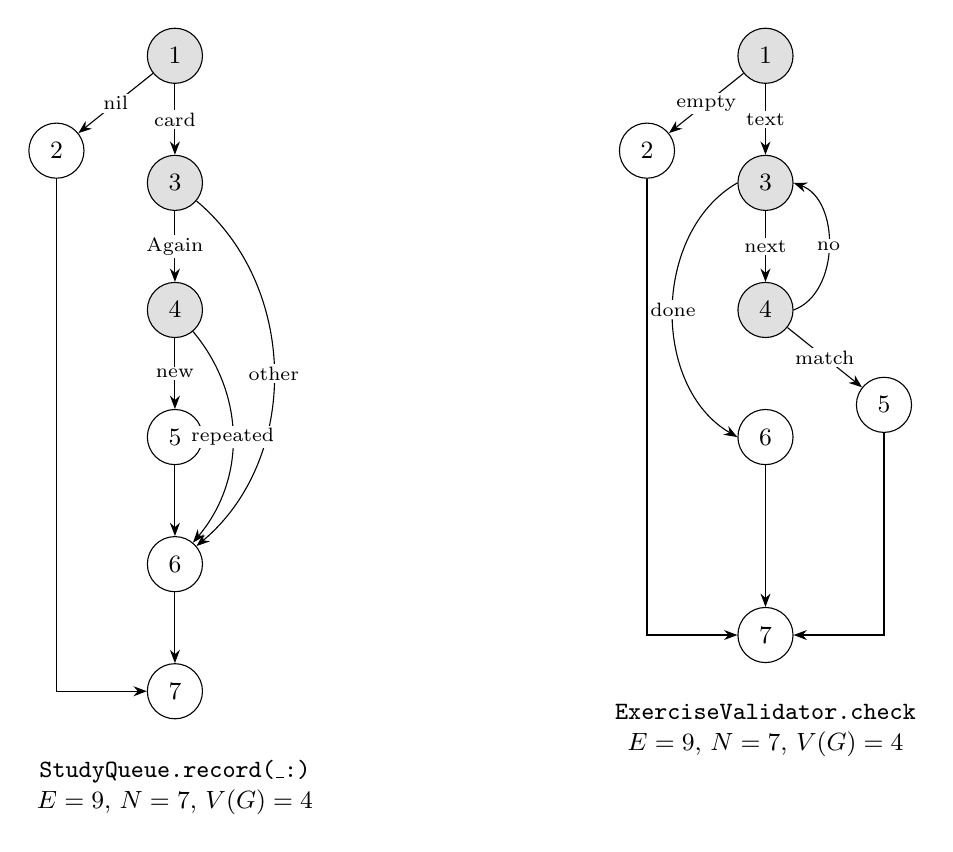
\begin{tikzpicture}[
    cfg/.style={circle, draw, minimum size=7mm, inner sep=0pt, font=\small},
    dec/.style={cfg, fill=black!12},
    lab/.style={font=\scriptsize, fill=white, inner sep=1pt},
    >=Stealth, node distance=9mm]
  % StudyQueue.record
  \node[dec] (a1) {1};
  \node[cfg, below left=7mm and 10mm of a1] (a2) {2};
  \node[dec, below=of a1] (a3) {3};
  \node[dec, below=of a3] (a4) {4};
  \node[cfg, below=of a4] (a5) {5};
  \node[cfg, below=of a5] (a6) {6};
  \node[cfg, below=of a6] (a7) {7};
  \draw[->] (a1) -- node[lab] {nil} (a2);
  \draw[->] (a1) -- node[lab] {card} (a3);
  \draw[->] (a3) -- node[lab] {Again} (a4);
  \draw[->] (a3) to[bend left=50] node[lab] {other} (a6);
  \draw[->] (a4) -- node[lab] {new} (a5);
  \draw[->] (a4) to[bend left=40] node[lab] {repeated} (a6);
  \draw[->] (a5) -- (a6);
  \draw[->] (a6) -- (a7);
  \draw[->] (a2) |- (a7);
  \node[below=4mm of a7, font=\small, align=center] {\texttt{StudyQueue.record(\_:)}\\$E=9$, $N=7$, $V(G)=4$};
  % ExerciseValidator.check
  \begin{scope}[xshift=7.5cm]
  \node[dec] (b1) {1};
  \node[cfg, below left=7mm and 10mm of b1] (b2) {2};
  \node[dec, below=of b1] (b3) {3};
  \node[dec, below=of b3] (b4) {4};
  \node[cfg, below right=7mm and 10mm of b4] (b5) {5};
  \node[cfg, below=of b4] (b6) {6};
  \node[cfg, below=18mm of b6] (b7) {7};
  \draw[->] (b1) -- node[lab] {empty} (b2);
  \draw[->] (b1) -- node[lab] {text} (b3);
  \draw[->] (b3) -- node[lab] {next} (b4);
  \draw[->] (b3.west) to[bend right=60] node[lab] {done} (b6.west);
  \draw[->] (b4) -- node[lab] {match} (b5);
  \draw[->] (b4.east) to[bend right=70] node[lab] {no} (b3.east);
  \draw[->] (b6) -- (b7);
  \draw[->] (b5) |- (b7);
  \draw[->] (b2) |- (b7);
  \node[below=4mm of b7, font=\small, align=center] {\texttt{ExerciseValidator.check}\\$E=9$, $N=7$, $V(G)=4$};
  \end{scope}
\end{tikzpicture}
\caption{Control flow graphs (shaded = decision). Left, \texttt{StudyQueue.record}: 1 card on screen?, 2 return, 3 rating is Again?, 4 not repeated yet?, 5 append and mark, 6 advance, 7 exit. Right, \texttt{ExerciseValidator.check}: 1 answer empty?, 2 return \texttt{.empty}, 3 another accepted answer?, 4 matches?, 5 return \texttt{.passed}, 6 return \texttt{.failed}, 7 exit.}
\label{fig:cfg}
\end{figure}

\begin{xltabular}{\textwidth}{@{}L{1.0cm} L{2.0cm} Y L{3.6cm} L{1.0cm}@{}}
\caption{Basis paths, inputs, and the tests that cover them}\label{tab:basispaths}\\
\toprule
\textbf{Path} & \textbf{Nodes} & \textbf{Input and expected result} & \textbf{Test} & \textbf{Result} \\
\midrule
\endfirsthead
\toprule
\textbf{Path} & \textbf{Nodes} & \textbf{Input and expected result} & \textbf{Test} & \textbf{Result} \\
\midrule
\endhead
\bottomrule
\endfoot
\multicolumn{5}{@{}l}{\textit{StudyQueue.record(\_:)} (\texttt{StudyQueueTests})} \\
Q1 & 1, 2, 7 & Finished queue $[a]$, \texttt{record(.again)}: nothing changes (position 1, cards $[a]$). & \texttt{recordingAfterFinishIsANoOp} & Pass \\
Q2 & 1, 3, 6, 7 & Queue $[a]$, \texttt{record(.good)}: position 1, no repeat, finished. Also Hard and Easy. & \texttt{goodRatingsWalkTheQueueAndFinish}, \texttt{onlyAgainRequeues} & Pass \\
Q3 & 1, 3, 4, 5, 6, 7 & Queue $[a, b]$, \texttt{record(.again)}: cards $[a, b, a]$, $a$ marked repeated, position 1. & \texttt{againRequeuesAtTheEndOnlyOnce} & Pass \\
Q4 & 1, 3, 4, 6, 7 & Same queue at the repeat of $a$, \texttt{record(.again)} again: cards stay $[a, b, a]$, finished. & \texttt{againRequeuesAtTheEndOnlyOnce} & Pass \\
\multicolumn{5}{@{}l}{\textit{ExerciseValidator.check(answer:accepted:)} (\texttt{ExerciseValidatorTests})} \\
V1 & 1, 2, 7 & Answer \texttt{""}, \texttt{"   "}, or only tabs and newlines: \texttt{.empty}. & \texttt{pathEmptyAnswer} (3 inputs) & Pass \\
V2 & 1, 3, 6, 7 & Answer \texttt{guard}, no accepted answers: \texttt{.failed}. & \texttt{pathNoAcceptedAnswers} & Pass \\
V3 & 1, 3, 4, 5, 7 & Answer \texttt{guard}, accepted \texttt{[guard]}: \texttt{.passed} on the first try. & \texttt{pathFirstAcceptedMatches} & Pass \\
V4 & 1, 3, 4, 3, 6, 7 & Answer \texttt{then}, accepted \texttt{[else]}: the loop ends with no match, \texttt{.failed}. & \texttt{pathNoMatchAfterLoop} & Pass \\
\end{xltabular}

The paths cover every node and every edge of both graphs, so statement and branch
coverage of the two methods is 100\%. Path coverage was not the only goal: further
tests check the cases the paths do not distinguish, such as a later accepted answer
matching (\texttt{laterAcceptedAnswerMatches}), spaces around operators
(\texttt{mid+1} accepted for \texttt{mid + 1}), and case sensitivity
(\texttt{Guard} fails).

\subsection{Integration Tests}\label{sec:integration}
\textbf{Plan (Activity~12.2).} The riskiest interface in Sprint~4 is the new progress
sync (FR-61): \texttt{SyncEngine} sends a \texttt{ProgressBatch} through
\texttt{SupabaseDataClient} to the \texttt{card\_progress},
\texttt{question\_progress}, and \texttt{topic\_progress} tables and pulls other
devices' rows back (Figure~\ref{fig:sequence3}). Both ends already existed, so the
team used the \emph{sandwich} strategy. The top half (the engine with the real
SwiftData store) runs against a stub, \texttt{MockRemoteStore}, which merges rows the
way the SQL triggers do and can fake a lost connection or a second device;
\texttt{MockAuth} stands in for a signed-in user. The bottom half (tables, triggers,
policies) is driven by SQL acting as the app: the pgTAP suite and the live RLS check.
The two halves meet in the client tests with a stubbed network and in a two-device
check on two Simulators. If something breaks, the layer that broke is known.

\textbf{Interface fault considered.} Swift's default encoder leaves a \texttt{nil}
field out of the JSON, and a Supabase upsert changes only the columns it receives.
When a card is un-retired, \texttt{retiredAt} is \texttt{nil}, so the server would keep
the old \texttt{retired\_at} and the other device would pull the card back as retired.
Each side passes its own unit tests; only the two together fail. Mitigation: the
progress row types encode every column, sending \texttt{nil} as an explicit JSON
\texttt{null}, and an integration test checks the request body
(\texttt{progressRowsSendRetiredAtAsExplicitNull}, added in Sprint~4 when the plan
showed it was missing).

\textbf{Entry criteria.} Unit tests of both sides pass with no open major defect; the
local Supabase stack runs with all 10 migrations; the stubs and drivers exist.
\textbf{Exit criteria.} All cases in Table~\ref{tab:inttests} pass; every defect found
is fixed and has a regression test; the known limits are written down (Reset Progress
is not sent to other devices; device clocks decide which review is the latest).

\begin{xltabular}{\textwidth}{@{}L{1.1cm} Y L{3.4cm} L{2.2cm}@{}}
\caption{Integration test cases and results}\label{tab:inttests}\\
\toprule
\textbf{ID} & \textbf{Components and check} & \textbf{Driver / stub} & \textbf{Result} \\
\midrule
\endfirsthead
\toprule
\textbf{ID} & \textbf{Components and check} & \textbf{Driver / stub} & \textbf{Result} \\
\midrule
\endhead
\bottomrule
\endfoot
IT-01 & \texttt{SyncEngine} + \texttt{SyncQueue} + \texttt{ConflictResolver} + SwiftData: push, pull, retry, conflict merge, offline queueing for decks and cards. & \texttt{SyncHarness}; \texttt{MockRemoteStore} & 25 of 25 pass \\
IT-02 & \texttt{SyncEngine} + \texttt{ProgressSync} + SwiftData: progress from a second device merges (newest review wins, unlocks never relock), offline then online. & \texttt{SyncHarness}; \texttt{MockRemoteStore.otherDeviceUpsert} & 13 of 13 pass \\
IT-03 & \texttt{SupabaseDataClient} + Supabase SDK: request bodies, explicit nulls, paging, error mapping. & Stubbed \texttt{URLProtocol} (\texttt{SupabaseTestClient}) & 11 of 11 pass \\
IT-04 & SwiftData schema V1--V8 + migration plan: each older store opens and keeps its data. & \texttt{MigrationTests} & 9 of 9 pass \\
IT-05 & Bundled content + store: seeding, the content stamp, starter decks, exercises. & \texttt{DataSeederTests}, \texttt{BundledContentStampTests} & 10 of 10 pass \\
IT-06 & App limits + database CHECK constraints agree. & \texttt{SupabaseSchemaTests}, \texttt{FlashcardSchemaFileTests} & 10 of 10 pass \\
IT-07 & Database tables + RLS + merge and rate-limit triggers, as a signed-in user. & pgTAP \texttt{rls.sql}, \texttt{progress.sql} & 75 of 75 pass (CI, Nov 14) \\
IT-08 & Live project: two users and a non-member against all 11 tables. & \texttt{rls\_live\_check.sql} & 0 of 57 fail (Nov 9) \\
IT-09 & Two Simulators, one account: a review on one shows on the other after one sync; sign-in with Google end to end. & By hand & Pass (Nov 10) \\
\end{xltabular}

IT-09 found BUG-02, a real fault of the kind the plan describes: both sides worked
alone, but together the sign-in failed (Table~\ref{tab:defects}).

\subsection{System Tests}\label{sec:systemtests}
System tests run the built app as a student would, on a Simulator, end to end.
Five are automated as XCUITests and run in CI; the rest are scripted walkthroughs
from Activity~13.1. The automated ones were run on the iPhone~17e, iPhone~17, and
iPhone~18 Pro Max Simulators; the audit walk (ST-06) runs in Light and Dark Mode.
\textbf{Entry:} unit and integration exit criteria met. \textbf{Exit:} every case
passes or has a logged defect with a decision.

\begin{xltabular}{\textwidth}{@{}L{1.0cm} L{3.0cm} Y L{2.4cm}@{}}
\caption{System test cases and results}\label{tab:systests}\\
\toprule
\textbf{ID} & \textbf{Scenario (FRs)} & \textbf{Steps and expected result} & \textbf{Result} \\
\midrule
\endfirsthead
\toprule
\textbf{ID} & \textbf{Scenario (FRs)} & \textbf{Steps and expected result} & \textbf{Result} \\
\midrule
\endhead
\bottomrule
\endfoot
ST-01 & Study a deck and resume (FR-16 to FR-18) & \texttt{StudySessionUITests}: open a starter deck, flip, rate by swipe, close mid-session, reopen; the session resumes on the same card. & Pass (automated) \\
ST-02 & Author and delete a deck (FR-05 to FR-13) & \texttt{DeckBuilderUITests}: create a deck with a Python snippet, save, find its tile; delete an unsynced deck from its detail screen. & Pass (automated) \\
ST-03 & Quiz with tiers, XP, streak, badge (FR-19 to FR-38) & New learner: onboarding, a 10-question quiz, then Home shows the XP, the streak, and the first badge; Medium unlocks after the retire threshold. & \tbd{result} \\
ST-04 & Offline use (FR-44 to FR-46, NFR-09) & Signed in, network off: study, answer a quiz, create a deck; network on: everything syncs, nothing is lost or duplicated. & \tbd{result} \\
ST-05 & Coding exercise (FR-39 to FR-41) & \texttt{ExerciseUITests}: Quiz tab, Coding Exercises, ``Exit early with guard''; one right and one wrong blank give Passed and Failed with the accepted answer; Try Again with both right gives ``All 2 tests passed''. & Pass (automated) \\
ST-06 & Every main screen is accessible (NFR-10 to NFR-12) & \texttt{AccessibilityAuditUITests}: walk 19 screens from onboarding to an answered question, run the system audit on each, in Light and Dark. & Pass, 0 open issues (automated) \\
ST-07 & Account, sync, groups (FR-01 to FR-03, FR-42, FR-50 to FR-53, FR-61) & Sign in with Google, sync, create a group, join it from a second account by code, see both on the weekly leaderboard, sign out. & Pass (Nov 10, by hand); \tbd{re-run} \\
\end{xltabular}

\subsection{Verification, Validation, and Acceptance}\label{sec:acceptance}
\textbf{Verification} asks whether the product was built right, against its
specification. Codey's verification is the traceability check: every requirement
names a test case, every test case names the suite that runs it
(Tables~\ref{tab:rtm}, \ref{tab:rtm-nfr}, \ref{tab:tcmap}), and the suites above
pass. All 66 functional requirements are implemented and traced to a passing test;
of the 31 active non-functional requirements, NFR-01 and NFR-28 wait on the device
measurement and NFR-24 on the traffic capture (Sections~\ref{sec:security} and
\ref{sec:performance}). Design reviews of each migration against the security
checklist (Table~\ref{tab:ssc}) are the other verification activity.

\textbf{Validation} asks whether the right product was built, for the client.
Following decision S34, it is done through acceptance tests rather than a peer
usability study: one scripted scenario per client mandate (Table~\ref{tab:accept}),
written from the mandate's wording, not from the code, and run by a team member who
did not build that feature, on a fresh install, as the demonstration will run.
\textbf{Plan:} run on Nov~19 (Activity~13.2); a scenario passes only if every
expected result is seen without help. \textbf{Exit:} all seven pass, or the client is
told which do not and why.

\begin{xltabular}{\textwidth}{@{}L{1.0cm} L{3.0cm} Y L{2.0cm}@{}}
\caption{Acceptance tests, one per client mandate}\label{tab:accept}\\
\toprule
\textbf{ID} & \textbf{Client mandate} & \textbf{Scenario and acceptance criterion} & \textbf{Result} \\
\midrule
\endfirsthead
\toprule
\textbf{ID} & \textbf{Client mandate} & \textbf{Scenario and acceptance criterion} & \textbf{Result} \\
\midrule
\endhead
\bottomrule
\endfoot
AT-01 & Adaptive tier rotation & Answer Easy questions in one topic until Medium unlocks; the next quiz mixes in Medium, and retired questions stop appearing. & \tbd{result} \\
AT-02 & XP, daily streaks, badges & Finish a study session and a quiz; XP and the streak rise on Home, and the first badge is awarded once. & \tbd{result} \\
AT-03 & Progress analytics and study plan & After two sessions, Home shows accuracy per topic and a study plan that names the weakest topic. & \tbd{result} \\
AT-04 & Offline use with cloud sync of decks & Create a deck in airplane mode; after reconnecting, it appears on a second device signed in to the same account. & \tbd{result} \\
AT-05 & Code-completion exercises & Open three exercises in different languages; wrong blanks show Failed and the accepted answer, right ones Passed, with an explanation. & \tbd{result} \\
AT-06 & Leaderboards and weekly challenges & Two accounts join one group; both appear on the weekly leaderboard with their XP, and the weekly challenge shows progress. & \tbd{result} \\
AT-07 & Offline sync of study results & Study on device A offline, reconnect; device B shows the same mastery and unlocks after one sync. & \tbd{result} \\
\end{xltabular}

\subsection{Defects Found}\label{sec:defects}
Table~\ref{tab:defects} lists the defects found in Sprint~4, how, and their fixes.
Each fix has a regression test, so the defect cannot return unnoticed. Three of the
entries are faults in the tests rather than the app; they are listed because a flaky
or blind test is a defect in the test plan.

\begin{xltabular}{\textwidth}{@{}L{1.1cm} Y L{2.4cm} Y L{2.2cm}@{}}
\caption{Defects found in Sprint 4}\label{tab:defects}\\
\toprule
\textbf{ID} & \textbf{Defect and cause} & \textbf{Found by} & \textbf{Fix} & \textbf{Regression test} \\
\midrule
\endfirsthead
\toprule
\textbf{ID} & \textbf{Defect and cause} & \textbf{Found by} & \textbf{Fix} & \textbf{Regression test} \\
\midrule
\endhead
\bottomrule
\endfoot
BUG-01 & Tapping ``Sign in with Google'' crashed (unrecognized selector): packages link statically, so the linker dropped an Objective-C category in AppAuth. & IT-09, Nov 10 & \texttt{-ObjC} linker flag on the app target (\texttt{1949cfe}). & \texttt{GoogleSignInLinkTests} \\
BUG-02 & Google signed in but Codey did not: Google Sign-In~10 always puts a nonce in the ID token, and Supabase rejects a token whose nonce it was not given. The free project had also paused after a week idle. & IT-09, Nov 10 & \texttt{SignInNonce}: SHA-256 to Google, raw value to Supabase; project restored; keep-alive job (\texttt{1949cfe}). & \texttt{SignInNonceTests} \\
BUG-03 & The exercise's code view was a selectable text view with no accessibility label, so VoiceOver read nothing for it. & ST-06 (audit), Nov 14 & Not selectable (the copy button covers copying) and labeled ``Swift code with 2 numbered blanks'' (\texttt{535911e}). & \texttt{AccessibilityAuditUITests} \\
TD-01 & No test checked that progress rows send \texttt{retired\_at} as an explicit null (the integration fault of Section~\ref{sec:integration}). & Activity~12.2 review & Test added (\texttt{535911e}). & \texttt{progressRowsSendRetiredAtAsExplicitNull} \\
TD-02 & \texttt{ExerciseUITests} failed on the iPhone~17e: the exercise row was not built yet in a lazy list below the fold. & ST-05, Nov 14 & Plain stack for the 12 rows; scroll until hittable (\texttt{535911e}). & ST-05 on 3 sizes \\
TD-03 & \texttt{ExerciseUITests} failed about 2 runs in 5 under load: the Simulator dropped a keystroke after the field had shown it. & Full CI-style run, Nov 14 & Hide the keyboard, re-check every blank's value, retype if needed, then tap Check (the same guard \texttt{DeckBuilderUITests} uses). & 5 of 5 consecutive passes \\
\end{xltabular}

% =====================================================================
\section{Concluding Remarks and Future Work}\label{sec:conclusion}
% =====================================================================
Codey now does what the client asked for. All 66 functional requirements are
implemented, including every client mandate: adaptive tier rotation, XP, streaks and
badges, progress analytics and a study plan, offline use with cloud sync of decks and,
since Sprint~4, of study results, leaderboards and weekly challenges, and
code-completion exercises. The app is covered by 388 unit tests, 6 UI tests over 19
screens, 75 database tests, and a 57-check live security test, all of which run with
one command and, except the live check, on every push. The team's main lessons were
practical ones: an integration can fail when both halves pass their own tests (the
explicit-null fault and BUG-02); a free backend that pauses when idle is a risk to
plan for, not a footnote (R11); and a test that fails one time in three is worth
fixing, because otherwise the team learns to ignore red.

Some things were deliberately left out, and are the natural next steps:
\begin{itemize}
  \item \textbf{Open-ended coding problems.} Exercises today compare each blank with
        accepted answers (R1). Running students' code would need a sandboxed
        execution service, which the Free plan and the client's no-cost constraint
        rule out for now.
  \item \textbf{Server-computed weekly XP.} The leaderboard trusts the client's XP,
        bounded only by the 600-XP-per-minute pace limit (R13, accepted). A ledger of
        answers kept and summed on the server would make the leaderboard
        tamper-proof.
  \item \textbf{Live performance tests.} NFR-02 was verified against a mock backend
        and NFR-32 was retired (S33). Dedicated test accounts would allow both, and
        a measurement on a cellular network.
  \item \textbf{Peer usability study.} Replaced by acceptance tests this sprint (S34);
        a task-success study with students would validate the design better than the
        team can.
  \item \textbf{Fuller sync.} Quiz history, daily activity, and badges stay on the
        device, and Reset Progress is not sent to other devices; device clocks decide
        the ``latest'' review.
  \item \textbf{Distribution.} Codey runs from Xcode. TestFlight distribution would
        need a paid developer account and moving the Google sign-in client to a Codey
        project.
\end{itemize}

% =====================================================================
\section*{Appendix A: Build Instructions}\label{sec:appA}
\addcontentsline{toc}{section}{Appendix A: Build Instructions}
% =====================================================================
These steps build and run the current version of Codey from a clean machine. Steps
A.2, A.3, A.8, and A.9 are repeated from a fresh checkout by continuous integration on
every push (\texttt{.github/workflows/test.yml}, Section~\ref{sec:vc}), on a clean
\texttt{macos-26} runner with no keys, which is the local-only mode of A.4; the last
such run on Nov 14, 2026 built the app and passed every unit and UI test. The database
steps were last run from scratch with the Supabase CLI on the same day (75 of 75 pgTAP
tests passed). \tbd{fresh-clone dry-run of the whole guide after the freeze, by whom}.

\textbf{A.1 Prerequisites.}
\begin{itemize}
  \item A Mac with Apple Silicon, running macOS 27 or later, with at least
        16 GB of memory.
  \item Xcode 27 (27.2 was used) from the Mac App Store, opened once to install its components, with
        the iOS 27 Simulator runtime (Xcode $\to$ Settings $\to$ Components).
  \item Homebrew (\texttt{https://brew.sh}), then Tuist:
        \texttt{brew install tuist} (version 4.214.1 was used).
  \item Git (included with Xcode's command line tools).
  \item Optional: the Supabase CLI (\texttt{brew install supabase/tap/supabase}, 3.1.0
        was used) and Docker or OrbStack for the local database tests, and
        \texttt{libpq} (\texttt{brew install libpq}) for \texttt{scripts/backup.sh}.
\end{itemize}

\textbf{A.2 Get the code.}
\begin{itemize}
  \item \texttt{git clone https://github.com/raajbanga/codey.git \&\& cd codey}
  \item \texttt{git checkout main} (the submitted state; \texttt{dev} has the latest work).
\end{itemize}

\textbf{A.3 Generate the Xcode workspace.}
\begin{itemize}
  \item \texttt{tuist install} downloads the pinned Swift packages
        (\texttt{Tuist/Package.swift}: Textual 0.5.0, Runestone 0.5.2,
        TreeSitterLanguages 0.1.10, supabase-swift 2.55.3, GoogleSignIn-iOS 10.0.0, and the
        test helpers xctest-dynamic-overlay 1.11.0 and swift-clocks 1.0.6).
  \item \texttt{tuist generate} creates \texttt{codey.xcworkspace} and opens it.
\end{itemize}

\textbf{A.4 Run without a backend (simplest).} Skip A.5--A.7. With no keys, the app
runs in local-only mode: everything except sign-in, sync, groups, and defect reports
works. Go to A.8.

\textbf{A.5 Secrets.} Copy \texttt{Config/Secrets.example.xcconfig} to
\texttt{Config/Secrets.xcconfig} (gitignored; never commit it) and fill in:
\begin{itemize}
  \item \texttt{SUPABASE\_URL}: Supabase $\to$ Project Settings $\to$ API $\to$ Project
        URL, written as \texttt{https:/\$()/\textit{ref}.supabase.co} because xcconfig
        treats \texttt{//} as a comment.
  \item \texttt{SUPABASE\_ANON\_KEY}: the \emph{anon public} key from the same page.
        Never use the \texttt{service\_role} key.
  \item \texttt{GOOGLE\_IOS\_CLIENT\_ID} and \texttt{GOOGLE\_REVERSED\_CLIENT\_ID}: the
        iOS OAuth client from A.7 and its reversed form
        (\texttt{com.googleusercontent.apps.\ldots}).
  \item \texttt{GOOGLE\_SERVER\_CLIENT\_ID}: the Web OAuth client from A.7.
\end{itemize}
Run \texttt{scripts/check-secrets.sh} to confirm nothing secret is tracked.

\textbf{A.6 Supabase project.}
\begin{itemize}
  \item Create a project on the Free plan (supabase.com), in the region nearest the
        users.
  \item Apply every file in \texttt{supabase/migrations} in filename order, either with
        the CLI (\texttt{supabase link -{}-project-ref \textit{ref}} then
        \texttt{supabase db push}) or by pasting each file into the SQL editor.
  \item Authentication $\to$ Sign In / Providers $\to$ Google: enable it and enter the
        Web client ID and secret from A.7; add the iOS client ID to the authorized
        client IDs.
  \item Run \texttt{supabase/checks/rls\_live\_check.sql} in the SQL editor; it must
        report 0 failed.
\end{itemize}
\texttt{supabase/README.md} has the same steps.

\textbf{A.7 Google Cloud OAuth.} In the Google Cloud console, create a project, configure
the OAuth consent screen in Testing mode with the team as test users, and create two
OAuth clients: an \emph{iOS} client with bundle ID \texttt{edu.wku.cs360.codey}, and a
\emph{Web} client whose ID and secret go into Supabase's Google provider.

\textbf{A.8 Build and run.} In Xcode, choose the \texttt{codey} scheme and an iPhone 17
Simulator, then Run (Command-R). From the command line:
\texttt{xcodebuild -workspace codey.xcworkspace -scheme codey -destination
'platform=iOS Simulator,name=iPhone 17' build}.

\textbf{A.9 Tests and checks.}
\begin{itemize}
  \item App tests: \texttt{scripts/test.sh} runs the unit tests and the accessibility
        audit on an iPhone~17 Simulator and prints each test's name, result, and time,
        then the failures and totals. Pass test filters to choose others, for example
        \texttt{scripts/test.sh -only-testing:codeyUITests} for all four UI suites (deck
        builder, study session, coding exercise, accessibility audit). Set
        \texttt{COVERAGE=1} for line coverage by folder, \texttt{CSV=\textit{path}} for
        per-suite counts, and \texttt{DESTINATION=\ldots} for another Simulator. The
        result bundle is \texttt{build/test.xcresult} and the full log
        \texttt{build/test.log}. On Xcode 27.1 and earlier, macOS may refuse the
        UI-test runner (R15); use Xcode 27.2.
  \item Database tests: \texttt{supabase db start} (builds a local database from the
        migrations), then \texttt{supabase test db} runs the 75 pgTAP tests in
        \texttt{supabase/tests}; \texttt{supabase stop} when done.
  \item Performance: \texttt{scripts/perf-report.sh} and, with the app installed on a
        booted Simulator, \texttt{scripts/perf-launch.sh}. Results go to
        \texttt{docs/source/perf/<tag>*.csv}; set \texttt{PERF\_TAG} (default
        \texttt{sprint4}) to keep each run apart.
  \item Repository checks: \texttt{scripts/check-imports.sh},
        \texttt{scripts/check-design-tokens.sh},
        \texttt{scripts/check-secrets.sh -{}-history},
        \texttt{scripts/check-release-build.sh}.
\end{itemize}

\textbf{A.10 Optional operations.} The coding exercises need no setup: they ship in
\texttt{codey/Resources/exercises.json} and are checked when the app loads them. Add the repository secrets \texttt{SUPABASE\_URL}
and \texttt{SUPABASE\_ANON\_KEY} on GitHub so the keep-alive workflow runs; back up
the database with \texttt{SUPABASE\_DB\_URL=\ldots{} scripts/backup.sh}.

\textbf{A.11 Troubleshooting.}
\begin{itemize}
  \item \emph{Packages fail to resolve or the project is stale}: \texttt{tuist clean},
        then \texttt{tuist install \&\& tuist generate}.
  \item \emph{Sign-in button missing}: a key in \texttt{Secrets.xcconfig} is empty, so
        the app is in local-only mode.
  \item \emph{Google sign-in returns to the app with an error}: the reversed client ID
        does not match the iOS client, or the account is not a listed test user.
\end{itemize}

% =====================================================================
\clearpage
\section*{Appendix B: Source Code and Configuration Files}\label{sec:appB}
\addcontentsline{toc}{section}{Appendix B: Source Code and Configuration Files}
% =====================================================================
This appendix lists every source and configuration file in the repository, one per
subsection, with line numbers; Table~\ref{tab:pattern-lines} refers to these line
numbers. It is generated by \texttt{scripts/gen-appendix-b.sh} from the final Sprint~4
commit \tbd{commit or tag after the freeze}. \texttt{Config/Secrets.xcconfig} (real keys) is never in the
repository and is not listed; \texttt{Secrets.example.xcconfig} shows its format.
Generated color sets and the app icon images are not source code and are omitted.

\setcounter{secnumdepth}{3}
\renewcommand{\thesubsubsection}{B.\arabic{subsubsection}}
\setcounter{subsubsection}{0}
\begingroup
\singlespacing
\ifcodelistings
\IfFileExists{generated/appendix_b.tex}{% Generated by scripts/gen-appendix-b.sh on 89d523b. Do not edit.
\subsection*{App}\addcontentsline{toc}{subsection}{App}
\subsubsection{codey/Sources/App/AppAppearance.swift}\label{appB:codey-Sources-App-AppAppearance-swift}
\lstinputlisting[language=Swift,basicstyle=\footnotesize\ttfamily]{../../codey/Sources/App/AppAppearance.swift}

\subsubsection{codey/Sources/App/AppConfig.swift}\label{appB:codey-Sources-App-AppConfig-swift}
\lstinputlisting[language=Swift,basicstyle=\footnotesize\ttfamily]{../../codey/Sources/App/AppConfig.swift}

\subsubsection{codey/Sources/App/AppLaunchOptions.swift}\label{appB:codey-Sources-App-AppLaunchOptions-swift}
\lstinputlisting[language=Swift,basicstyle=\footnotesize\ttfamily]{../../codey/Sources/App/AppLaunchOptions.swift}

\subsubsection{codey/Sources/App/LaunchTimer.swift}\label{appB:codey-Sources-App-LaunchTimer-swift}
\lstinputlisting[language=Swift,basicstyle=\footnotesize\ttfamily]{../../codey/Sources/App/LaunchTimer.swift}

\subsubsection{codey/Sources/App/LoadingView.swift}\label{appB:codey-Sources-App-LoadingView-swift}
\lstinputlisting[language=Swift,basicstyle=\footnotesize\ttfamily]{../../codey/Sources/App/LoadingView.swift}

\subsubsection{codey/Sources/App/Logging.swift}\label{appB:codey-Sources-App-Logging-swift}
\lstinputlisting[language=Swift,basicstyle=\footnotesize\ttfamily]{../../codey/Sources/App/Logging.swift}

\subsubsection{codey/Sources/CodeyApp.swift}\label{appB:codey-Sources-CodeyApp-swift}
\lstinputlisting[language=Swift,basicstyle=\footnotesize\ttfamily]{../../codey/Sources/CodeyApp.swift}

\subsubsection{codey/Sources/ContentView.swift}\label{appB:codey-Sources-ContentView-swift}
\lstinputlisting[language=Swift,basicstyle=\footnotesize\ttfamily]{../../codey/Sources/ContentView.swift}

\subsection*{Models}\addcontentsline{toc}{subsection}{Models}
\subsubsection{codey/Sources/Models/Decks/CardRating.swift}\label{appB:codey-Sources-Models-Decks-CardRating-swift}
\lstinputlisting[language=Swift,basicstyle=\footnotesize\ttfamily]{../../codey/Sources/Models/Decks/CardRating.swift}

\subsubsection{codey/Sources/Models/Decks/CodeLanguage.swift}\label{appB:codey-Sources-Models-Decks-CodeLanguage-swift}
\lstinputlisting[language=Swift,basicstyle=\footnotesize\ttfamily]{../../codey/Sources/Models/Decks/CodeLanguage.swift}

\subsubsection{codey/Sources/Models/Decks/CodeSnippet.swift}\label{appB:codey-Sources-Models-Decks-CodeSnippet-swift}
\lstinputlisting[language=Swift,basicstyle=\footnotesize\ttfamily]{../../codey/Sources/Models/Decks/CodeSnippet.swift}

\subsubsection{codey/Sources/Models/Decks/DeckOrigin.swift}\label{appB:codey-Sources-Models-Decks-DeckOrigin-swift}
\lstinputlisting[language=Swift,basicstyle=\footnotesize\ttfamily]{../../codey/Sources/Models/Decks/DeckOrigin.swift}

\subsubsection{codey/Sources/Models/Decks/Flashcard.swift}\label{appB:codey-Sources-Models-Decks-Flashcard-swift}
\lstinputlisting[language=Swift,basicstyle=\footnotesize\ttfamily]{../../codey/Sources/Models/Decks/Flashcard.swift}

\subsubsection{codey/Sources/Models/Decks/FlashcardDeck.swift}\label{appB:codey-Sources-Models-Decks-FlashcardDeck-swift}
\lstinputlisting[language=Swift,basicstyle=\footnotesize\ttfamily]{../../codey/Sources/Models/Decks/FlashcardDeck.swift}

\subsubsection{codey/Sources/Models/ProfileAvatar.swift}\label{appB:codey-Sources-Models-ProfileAvatar-swift}
\lstinputlisting[language=Swift,basicstyle=\footnotesize\ttfamily]{../../codey/Sources/Models/ProfileAvatar.swift}

\subsubsection{codey/Sources/Models/Progress/BadgeAward.swift}\label{appB:codey-Sources-Models-Progress-BadgeAward-swift}
\lstinputlisting[language=Swift,basicstyle=\footnotesize\ttfamily]{../../codey/Sources/Models/Progress/BadgeAward.swift}

\subsubsection{codey/Sources/Models/Progress/DailyActivity.swift}\label{appB:codey-Sources-Models-Progress-DailyActivity-swift}
\lstinputlisting[language=Swift,basicstyle=\footnotesize\ttfamily]{../../codey/Sources/Models/Progress/DailyActivity.swift}

\subsubsection{codey/Sources/Models/Progress/QuestionProgress.swift}\label{appB:codey-Sources-Models-Progress-QuestionProgress-swift}
\lstinputlisting[language=Swift,basicstyle=\footnotesize\ttfamily]{../../codey/Sources/Models/Progress/QuestionProgress.swift}

\subsubsection{codey/Sources/Models/Progress/QuizAnswerRecord.swift}\label{appB:codey-Sources-Models-Progress-QuizAnswerRecord-swift}
\lstinputlisting[language=Swift,basicstyle=\footnotesize\ttfamily]{../../codey/Sources/Models/Progress/QuizAnswerRecord.swift}

\subsubsection{codey/Sources/Models/Progress/StudyProgressSnapshot.swift}\label{appB:codey-Sources-Models-Progress-StudyProgressSnapshot-swift}
\lstinputlisting[language=Swift,basicstyle=\footnotesize\ttfamily]{../../codey/Sources/Models/Progress/StudyProgressSnapshot.swift}

\subsubsection{codey/Sources/Models/Progress/TopicProgress.swift}\label{appB:codey-Sources-Models-Progress-TopicProgress-swift}
\lstinputlisting[language=Swift,basicstyle=\footnotesize\ttfamily]{../../codey/Sources/Models/Progress/TopicProgress.swift}

\subsubsection{codey/Sources/Models/Question.swift}\label{appB:codey-Sources-Models-Question-swift}
\lstinputlisting[language=Swift,basicstyle=\footnotesize\ttfamily]{../../codey/Sources/Models/Question.swift}

\subsubsection{codey/Sources/Models/Schema/CodeyMigrationPlan.swift}\label{appB:codey-Sources-Models-Schema-CodeyMigrationPlan-swift}
\lstinputlisting[language=Swift,basicstyle=\footnotesize\ttfamily]{../../codey/Sources/Models/Schema/CodeyMigrationPlan.swift}

\subsubsection{codey/Sources/Models/Schema/CodeySchemaV1.swift}\label{appB:codey-Sources-Models-Schema-CodeySchemaV1-swift}
\lstinputlisting[language=Swift,basicstyle=\footnotesize\ttfamily]{../../codey/Sources/Models/Schema/CodeySchemaV1.swift}

\subsubsection{codey/Sources/Models/Schema/CodeySchemaV2.swift}\label{appB:codey-Sources-Models-Schema-CodeySchemaV2-swift}
\lstinputlisting[language=Swift,basicstyle=\footnotesize\ttfamily]{../../codey/Sources/Models/Schema/CodeySchemaV2.swift}

\subsubsection{codey/Sources/Models/Schema/CodeySchemaV3.swift}\label{appB:codey-Sources-Models-Schema-CodeySchemaV3-swift}
\lstinputlisting[language=Swift,basicstyle=\footnotesize\ttfamily]{../../codey/Sources/Models/Schema/CodeySchemaV3.swift}

\subsubsection{codey/Sources/Models/Schema/CodeySchemaV4.swift}\label{appB:codey-Sources-Models-Schema-CodeySchemaV4-swift}
\lstinputlisting[language=Swift,basicstyle=\footnotesize\ttfamily]{../../codey/Sources/Models/Schema/CodeySchemaV4.swift}

\subsubsection{codey/Sources/Models/Schema/CodeySchemaV5.swift}\label{appB:codey-Sources-Models-Schema-CodeySchemaV5-swift}
\lstinputlisting[language=Swift,basicstyle=\footnotesize\ttfamily]{../../codey/Sources/Models/Schema/CodeySchemaV5.swift}

\subsubsection{codey/Sources/Models/Schema/CodeySchemaV6.swift}\label{appB:codey-Sources-Models-Schema-CodeySchemaV6-swift}
\lstinputlisting[language=Swift,basicstyle=\footnotesize\ttfamily]{../../codey/Sources/Models/Schema/CodeySchemaV6.swift}

\subsubsection{codey/Sources/Models/Schema/CodeySchemaV7.swift}\label{appB:codey-Sources-Models-Schema-CodeySchemaV7-swift}
\lstinputlisting[language=Swift,basicstyle=\footnotesize\ttfamily]{../../codey/Sources/Models/Schema/CodeySchemaV7.swift}

\subsubsection{codey/Sources/Models/Schema/CodeySchemaV8.swift}\label{appB:codey-Sources-Models-Schema-CodeySchemaV8-swift}
\lstinputlisting[language=Swift,basicstyle=\footnotesize\ttfamily]{../../codey/Sources/Models/Schema/CodeySchemaV8.swift}

\subsubsection{codey/Sources/Models/Sync/DeckSyncStateKind.swift}\label{appB:codey-Sources-Models-Sync-DeckSyncStateKind-swift}
\lstinputlisting[language=Swift,basicstyle=\footnotesize\ttfamily]{../../codey/Sources/Models/Sync/DeckSyncStateKind.swift}

\subsubsection{codey/Sources/Models/Sync/SyncOperation.swift}\label{appB:codey-Sources-Models-Sync-SyncOperation-swift}
\lstinputlisting[language=Swift,basicstyle=\footnotesize\ttfamily]{../../codey/Sources/Models/Sync/SyncOperation.swift}

\subsubsection{codey/Sources/Models/Topic.swift}\label{appB:codey-Sources-Models-Topic-swift}
\lstinputlisting[language=Swift,basicstyle=\footnotesize\ttfamily]{../../codey/Sources/Models/Topic.swift}

\subsubsection{codey/Sources/Models/UserProfile.swift}\label{appB:codey-Sources-Models-UserProfile-swift}
\lstinputlisting[language=Swift,basicstyle=\footnotesize\ttfamily]{../../codey/Sources/Models/UserProfile.swift}

\subsection*{View models}\addcontentsline{toc}{subsection}{View models}
\subsubsection{codey/Sources/ViewModels/DeckDraft.swift}\label{appB:codey-Sources-ViewModels-DeckDraft-swift}
\lstinputlisting[language=Swift,basicstyle=\footnotesize\ttfamily]{../../codey/Sources/ViewModels/DeckDraft.swift}

\subsubsection{codey/Sources/ViewModels/DeckViewModel.swift}\label{appB:codey-Sources-ViewModels-DeckViewModel-swift}
\lstinputlisting[language=Swift,basicstyle=\footnotesize\ttfamily]{../../codey/Sources/ViewModels/DeckViewModel.swift}

\subsubsection{codey/Sources/ViewModels/QuizViewModel.swift}\label{appB:codey-Sources-ViewModels-QuizViewModel-swift}
\lstinputlisting[language=Swift,basicstyle=\footnotesize\ttfamily]{../../codey/Sources/ViewModels/QuizViewModel.swift}

\subsubsection{codey/Sources/ViewModels/StudySessionViewModel.swift}\label{appB:codey-Sources-ViewModels-StudySessionViewModel-swift}
\lstinputlisting[language=Swift,basicstyle=\footnotesize\ttfamily]{../../codey/Sources/ViewModels/StudySessionViewModel.swift}

\subsection*{Services}\addcontentsline{toc}{subsection}{Services}
\subsubsection{codey/Sources/Services/Backend/AuthState.swift}\label{appB:codey-Sources-Services-Backend-AuthState-swift}
\lstinputlisting[language=Swift,basicstyle=\footnotesize\ttfamily]{../../codey/Sources/Services/Backend/AuthState.swift}

\subsubsection{codey/Sources/Services/Backend/BackendFacade+Decks.swift}\label{appB:codey-Sources-Services-Backend-BackendFacade-Decks-swift}
\lstinputlisting[language=Swift,basicstyle=\footnotesize\ttfamily]{../../codey/Sources/Services/Backend/BackendFacade+Decks.swift}

\subsubsection{codey/Sources/Services/Backend/BackendFacade+Groups.swift}\label{appB:codey-Sources-Services-Backend-BackendFacade-Groups-swift}
\lstinputlisting[language=Swift,basicstyle=\footnotesize\ttfamily]{../../codey/Sources/Services/Backend/BackendFacade+Groups.swift}

\subsubsection{codey/Sources/Services/Backend/BackendFacade+Profile.swift}\label{appB:codey-Sources-Services-Backend-BackendFacade-Profile-swift}
\lstinputlisting[language=Swift,basicstyle=\footnotesize\ttfamily]{../../codey/Sources/Services/Backend/BackendFacade+Profile.swift}

\subsubsection{codey/Sources/Services/Backend/BackendFacade.swift}\label{appB:codey-Sources-Services-Backend-BackendFacade-swift}
\lstinputlisting[language=Swift,basicstyle=\footnotesize\ttfamily]{../../codey/Sources/Services/Backend/BackendFacade.swift}

\subsubsection{codey/Sources/Services/Backend/BackendProtocols.swift}\label{appB:codey-Sources-Services-Backend-BackendProtocols-swift}
\lstinputlisting[language=Swift,basicstyle=\footnotesize\ttfamily]{../../codey/Sources/Services/Backend/BackendProtocols.swift}

\subsubsection{codey/Sources/Services/Backend/DeckBackend.swift}\label{appB:codey-Sources-Services-Backend-DeckBackend-swift}
\lstinputlisting[language=Swift,basicstyle=\footnotesize\ttfamily]{../../codey/Sources/Services/Backend/DeckBackend.swift}

\subsubsection{codey/Sources/Services/Backend/GroupCache.swift}\label{appB:codey-Sources-Services-Backend-GroupCache-swift}
\lstinputlisting[language=Swift,basicstyle=\footnotesize\ttfamily]{../../codey/Sources/Services/Backend/GroupCache.swift}

\subsubsection{codey/Sources/Services/Backend/NetworkMonitor.swift}\label{appB:codey-Sources-Services-Backend-NetworkMonitor-swift}
\lstinputlisting[language=Swift,basicstyle=\footnotesize\ttfamily]{../../codey/Sources/Services/Backend/NetworkMonitor.swift}

\subsubsection{codey/Sources/Services/Backend/Supabase/KeychainSessionStorage.swift}\label{appB:codey-Sources-Services-Backend-Supabase-KeychainSessionStorage-swift}
\lstinputlisting[language=Swift,basicstyle=\footnotesize\ttfamily]{../../codey/Sources/Services/Backend/Supabase/KeychainSessionStorage.swift}

\subsubsection{codey/Sources/Services/Backend/Supabase/SupabaseAuthProvider.swift}\label{appB:codey-Sources-Services-Backend-Supabase-SupabaseAuthProvider-swift}
\lstinputlisting[language=Swift,basicstyle=\footnotesize\ttfamily]{../../codey/Sources/Services/Backend/Supabase/SupabaseAuthProvider.swift}

\subsubsection{codey/Sources/Services/Backend/Supabase/SupabaseDataClient.swift}\label{appB:codey-Sources-Services-Backend-Supabase-SupabaseDataClient-swift}
\lstinputlisting[language=Swift,basicstyle=\footnotesize\ttfamily]{../../codey/Sources/Services/Backend/Supabase/SupabaseDataClient.swift}

\subsubsection{codey/Sources/Services/Backend/Supabase/SupabaseServices.swift}\label{appB:codey-Sources-Services-Backend-Supabase-SupabaseServices-swift}
\lstinputlisting[language=Swift,basicstyle=\footnotesize\ttfamily]{../../codey/Sources/Services/Backend/Supabase/SupabaseServices.swift}

\subsubsection{codey/Sources/Services/Backend/Supabase/SupabaseTestAccounts.swift}\label{appB:codey-Sources-Services-Backend-Supabase-SupabaseTestAccounts-swift}
\lstinputlisting[language=Swift,basicstyle=\footnotesize\ttfamily]{../../codey/Sources/Services/Backend/Supabase/SupabaseTestAccounts.swift}

\subsubsection{codey/Sources/Services/Backend/SwiftDataService.swift}\label{appB:codey-Sources-Services-Backend-SwiftDataService-swift}
\lstinputlisting[language=Swift,basicstyle=\footnotesize\ttfamily]{../../codey/Sources/Services/Backend/SwiftDataService.swift}

\subsubsection{codey/Sources/Services/BundledContentStamp.swift}\label{appB:codey-Sources-Services-BundledContentStamp-swift}
\lstinputlisting[language=Swift,basicstyle=\footnotesize\ttfamily]{../../codey/Sources/Services/BundledContentStamp.swift}

\subsubsection{codey/Sources/Services/DataSeeder.swift}\label{appB:codey-Sources-Services-DataSeeder-swift}
\lstinputlisting[language=Swift,basicstyle=\footnotesize\ttfamily]{../../codey/Sources/Services/DataSeeder.swift}

\subsubsection{codey/Sources/Services/Decks/FlashcardFactory.swift}\label{appB:codey-Sources-Services-Decks-FlashcardFactory-swift}
\lstinputlisting[language=Swift,basicstyle=\footnotesize\ttfamily]{../../codey/Sources/Services/Decks/FlashcardFactory.swift}

\subsubsection{codey/Sources/Services/Decks/FlashcardPayload.swift}\label{appB:codey-Sources-Services-Decks-FlashcardPayload-swift}
\lstinputlisting[language=Swift,basicstyle=\footnotesize\ttfamily]{../../codey/Sources/Services/Decks/FlashcardPayload.swift}

\subsubsection{codey/Sources/Services/Decks/ModelValidator.swift}\label{appB:codey-Sources-Services-Decks-ModelValidator-swift}
\lstinputlisting[language=Swift,basicstyle=\footnotesize\ttfamily]{../../codey/Sources/Services/Decks/ModelValidator.swift}

\subsubsection{codey/Sources/Services/Decks/StableID.swift}\label{appB:codey-Sources-Services-Decks-StableID-swift}
\lstinputlisting[language=Swift,basicstyle=\footnotesize\ttfamily]{../../codey/Sources/Services/Decks/StableID.swift}

\subsubsection{codey/Sources/Services/Decks/StarterDeckLoader.swift}\label{appB:codey-Sources-Services-Decks-StarterDeckLoader-swift}
\lstinputlisting[language=Swift,basicstyle=\footnotesize\ttfamily]{../../codey/Sources/Services/Decks/StarterDeckLoader.swift}

\subsubsection{codey/Sources/Services/Gamification/BadgeEvaluator.swift}\label{appB:codey-Sources-Services-Gamification-BadgeEvaluator-swift}
\lstinputlisting[language=Swift,basicstyle=\footnotesize\ttfamily]{../../codey/Sources/Services/Gamification/BadgeEvaluator.swift}

\subsubsection{codey/Sources/Services/Gamification/LevelCalculator.swift}\label{appB:codey-Sources-Services-Gamification-LevelCalculator-swift}
\lstinputlisting[language=Swift,basicstyle=\footnotesize\ttfamily]{../../codey/Sources/Services/Gamification/LevelCalculator.swift}

\subsubsection{codey/Sources/Services/Gamification/StreakCalculator.swift}\label{appB:codey-Sources-Services-Gamification-StreakCalculator-swift}
\lstinputlisting[language=Swift,basicstyle=\footnotesize\ttfamily]{../../codey/Sources/Services/Gamification/StreakCalculator.swift}

\subsubsection{codey/Sources/Services/Gamification/WeeklyChallenge.swift}\label{appB:codey-Sources-Services-Gamification-WeeklyChallenge-swift}
\lstinputlisting[language=Swift,basicstyle=\footnotesize\ttfamily]{../../codey/Sources/Services/Gamification/WeeklyChallenge.swift}

\subsubsection{codey/Sources/Services/Gamification/WeeklyXPStore.swift}\label{appB:codey-Sources-Services-Gamification-WeeklyXPStore-swift}
\lstinputlisting[language=Swift,basicstyle=\footnotesize\ttfamily]{../../codey/Sources/Services/Gamification/WeeklyXPStore.swift}

\subsubsection{codey/Sources/Services/Gamification/XPPolicy.swift}\label{appB:codey-Sources-Services-Gamification-XPPolicy-swift}
\lstinputlisting[language=Swift,basicstyle=\footnotesize\ttfamily]{../../codey/Sources/Services/Gamification/XPPolicy.swift}

\subsubsection{codey/Sources/Services/LocalDataReset.swift}\label{appB:codey-Sources-Services-LocalDataReset-swift}
\lstinputlisting[language=Swift,basicstyle=\footnotesize\ttfamily]{../../codey/Sources/Services/LocalDataReset.swift}

\subsubsection{codey/Sources/Services/ModelContainerFactory.swift}\label{appB:codey-Sources-Services-ModelContainerFactory-swift}
\lstinputlisting[language=Swift,basicstyle=\footnotesize\ttfamily]{../../codey/Sources/Services/ModelContainerFactory.swift}

\subsubsection{codey/Sources/Services/Practice/GatingConfig.swift}\label{appB:codey-Sources-Services-Practice-GatingConfig-swift}
\lstinputlisting[language=Swift,basicstyle=\footnotesize\ttfamily]{../../codey/Sources/Services/Practice/GatingConfig.swift}

\subsubsection{codey/Sources/Services/Practice/LeaderboardRanking.swift}\label{appB:codey-Sources-Services-Practice-LeaderboardRanking-swift}
\lstinputlisting[language=Swift,basicstyle=\footnotesize\ttfamily]{../../codey/Sources/Services/Practice/LeaderboardRanking.swift}

\subsubsection{codey/Sources/Services/Practice/QuestionPool.swift}\label{appB:codey-Sources-Services-Practice-QuestionPool-swift}
\lstinputlisting[language=Swift,basicstyle=\footnotesize\ttfamily]{../../codey/Sources/Services/Practice/QuestionPool.swift}

\subsubsection{codey/Sources/Services/Practice/QuizProgressStore.swift}\label{appB:codey-Sources-Services-Practice-QuizProgressStore-swift}
\lstinputlisting[language=Swift,basicstyle=\footnotesize\ttfamily]{../../codey/Sources/Services/Practice/QuizProgressStore.swift}

\subsubsection{codey/Sources/Services/Practice/SeededGenerator.swift}\label{appB:codey-Sources-Services-Practice-SeededGenerator-swift}
\lstinputlisting[language=Swift,basicstyle=\footnotesize\ttfamily]{../../codey/Sources/Services/Practice/SeededGenerator.swift}

\subsubsection{codey/Sources/Services/Practice/StudyPlanBuilder.swift}\label{appB:codey-Sources-Services-Practice-StudyPlanBuilder-swift}
\lstinputlisting[language=Swift,basicstyle=\footnotesize\ttfamily]{../../codey/Sources/Services/Practice/StudyPlanBuilder.swift}

\subsubsection{codey/Sources/Services/Practice/TierGate.swift}\label{appB:codey-Sources-Services-Practice-TierGate-swift}
\lstinputlisting[language=Swift,basicstyle=\footnotesize\ttfamily]{../../codey/Sources/Services/Practice/TierGate.swift}

\subsubsection{codey/Sources/Services/QuestionBankLoader.swift}\label{appB:codey-Sources-Services-QuestionBankLoader-swift}
\lstinputlisting[language=Swift,basicstyle=\footnotesize\ttfamily]{../../codey/Sources/Services/QuestionBankLoader.swift}

\subsubsection{codey/Sources/Services/Study/StudyPool.swift}\label{appB:codey-Sources-Services-Study-StudyPool-swift}
\lstinputlisting[language=Swift,basicstyle=\footnotesize\ttfamily]{../../codey/Sources/Services/Study/StudyPool.swift}

\subsubsection{codey/Sources/Services/Study/StudyQueue.swift}\label{appB:codey-Sources-Services-Study-StudyQueue-swift}
\lstinputlisting[language=Swift,basicstyle=\footnotesize\ttfamily]{../../codey/Sources/Services/Study/StudyQueue.swift}

\subsubsection{codey/Sources/Services/Sync/ConflictResolver.swift}\label{appB:codey-Sources-Services-Sync-ConflictResolver-swift}
\lstinputlisting[language=Swift,basicstyle=\footnotesize\ttfamily]{../../codey/Sources/Services/Sync/ConflictResolver.swift}

\subsubsection{codey/Sources/Services/Sync/DeckSyncState.swift}\label{appB:codey-Sources-Services-Sync-DeckSyncState-swift}
\lstinputlisting[language=Swift,basicstyle=\footnotesize\ttfamily]{../../codey/Sources/Services/Sync/DeckSyncState.swift}

\subsubsection{codey/Sources/Services/Sync/SyncCursorStore.swift}\label{appB:codey-Sources-Services-Sync-SyncCursorStore-swift}
\lstinputlisting[language=Swift,basicstyle=\footnotesize\ttfamily]{../../codey/Sources/Services/Sync/SyncCursorStore.swift}

\subsubsection{codey/Sources/Services/Sync/SyncEngine.swift}\label{appB:codey-Sources-Services-Sync-SyncEngine-swift}
\lstinputlisting[language=Swift,basicstyle=\footnotesize\ttfamily]{../../codey/Sources/Services/Sync/SyncEngine.swift}

\subsubsection{codey/Sources/Services/Sync/SyncQueue.swift}\label{appB:codey-Sources-Services-Sync-SyncQueue-swift}
\lstinputlisting[language=Swift,basicstyle=\footnotesize\ttfamily]{../../codey/Sources/Services/Sync/SyncQueue.swift}

\subsection*{Design system}\addcontentsline{toc}{subsection}{Design system}
\subsubsection{codey/Sources/DesignSystem/CodeEditor/CodeEditorView.swift}\label{appB:codey-Sources-DesignSystem-CodeEditor-CodeEditorView-swift}
\lstinputlisting[language=Swift,basicstyle=\footnotesize\ttfamily]{../../codey/Sources/DesignSystem/CodeEditor/CodeEditorView.swift}

\subsubsection{codey/Sources/DesignSystem/CodeEditor/CodeyRunestoneTheme.swift}\label{appB:codey-Sources-DesignSystem-CodeEditor-CodeyRunestoneTheme-swift}
\lstinputlisting[language=Swift,basicstyle=\footnotesize\ttfamily]{../../codey/Sources/DesignSystem/CodeEditor/CodeyRunestoneTheme.swift}

\subsubsection{codey/Sources/DesignSystem/Components/AnswerOptionRow.swift}\label{appB:codey-Sources-DesignSystem-Components-AnswerOptionRow-swift}
\lstinputlisting[language=Swift,basicstyle=\footnotesize\ttfamily]{../../codey/Sources/DesignSystem/Components/AnswerOptionRow.swift}

\subsubsection{codey/Sources/DesignSystem/Components/AppGlyph.swift}\label{appB:codey-Sources-DesignSystem-Components-AppGlyph-swift}
\lstinputlisting[language=Swift,basicstyle=\footnotesize\ttfamily]{../../codey/Sources/DesignSystem/Components/AppGlyph.swift}

\subsubsection{codey/Sources/DesignSystem/Components/CelebrationOverlay.swift}\label{appB:codey-Sources-DesignSystem-Components-CelebrationOverlay-swift}
\lstinputlisting[language=Swift,basicstyle=\footnotesize\ttfamily]{../../codey/Sources/DesignSystem/Components/CelebrationOverlay.swift}

\subsubsection{codey/Sources/DesignSystem/Components/CloseButton.swift}\label{appB:codey-Sources-DesignSystem-Components-CloseButton-swift}
\lstinputlisting[language=Swift,basicstyle=\footnotesize\ttfamily]{../../codey/Sources/DesignSystem/Components/CloseButton.swift}

\subsubsection{codey/Sources/DesignSystem/Components/CodeyButton.swift}\label{appB:codey-Sources-DesignSystem-Components-CodeyButton-swift}
\lstinputlisting[language=Swift,basicstyle=\footnotesize\ttfamily]{../../codey/Sources/DesignSystem/Components/CodeyButton.swift}

\subsubsection{codey/Sources/DesignSystem/Components/CodeyCard.swift}\label{appB:codey-Sources-DesignSystem-Components-CodeyCard-swift}
\lstinputlisting[language=Swift,basicstyle=\footnotesize\ttfamily]{../../codey/Sources/DesignSystem/Components/CodeyCard.swift}

\subsubsection{codey/Sources/DesignSystem/Components/CodeyChip.swift}\label{appB:codey-Sources-DesignSystem-Components-CodeyChip-swift}
\lstinputlisting[language=Swift,basicstyle=\footnotesize\ttfamily]{../../codey/Sources/DesignSystem/Components/CodeyChip.swift}

\subsubsection{codey/Sources/DesignSystem/Components/EmptyStateView.swift}\label{appB:codey-Sources-DesignSystem-Components-EmptyStateView-swift}
\lstinputlisting[language=Swift,basicstyle=\footnotesize\ttfamily]{../../codey/Sources/DesignSystem/Components/EmptyStateView.swift}

\subsubsection{codey/Sources/DesignSystem/Components/FormFeedback.swift}\label{appB:codey-Sources-DesignSystem-Components-FormFeedback-swift}
\lstinputlisting[language=Swift,basicstyle=\footnotesize\ttfamily]{../../codey/Sources/DesignSystem/Components/FormFeedback.swift}

\subsubsection{codey/Sources/DesignSystem/Components/IconTile.swift}\label{appB:codey-Sources-DesignSystem-Components-IconTile-swift}
\lstinputlisting[language=Swift,basicstyle=\footnotesize\ttfamily]{../../codey/Sources/DesignSystem/Components/IconTile.swift}

\subsubsection{codey/Sources/DesignSystem/Components/MasteryDots.swift}\label{appB:codey-Sources-DesignSystem-Components-MasteryDots-swift}
\lstinputlisting[language=Swift,basicstyle=\footnotesize\ttfamily]{../../codey/Sources/DesignSystem/Components/MasteryDots.swift}

\subsubsection{codey/Sources/DesignSystem/Components/ProgressBar.swift}\label{appB:codey-Sources-DesignSystem-Components-ProgressBar-swift}
\lstinputlisting[language=Swift,basicstyle=\footnotesize\ttfamily]{../../codey/Sources/DesignSystem/Components/ProgressBar.swift}

\subsubsection{codey/Sources/DesignSystem/Components/ProgressRing.swift}\label{appB:codey-Sources-DesignSystem-Components-ProgressRing-swift}
\lstinputlisting[language=Swift,basicstyle=\footnotesize\ttfamily]{../../codey/Sources/DesignSystem/Components/ProgressRing.swift}

\subsubsection{codey/Sources/DesignSystem/Components/StatTile.swift}\label{appB:codey-Sources-DesignSystem-Components-StatTile-swift}
\lstinputlisting[language=Swift,basicstyle=\footnotesize\ttfamily]{../../codey/Sources/DesignSystem/Components/StatTile.swift}

\subsubsection{codey/Sources/DesignSystem/Components/TierChipRow.swift}\label{appB:codey-Sources-DesignSystem-Components-TierChipRow-swift}
\lstinputlisting[language=Swift,basicstyle=\footnotesize\ttfamily]{../../codey/Sources/DesignSystem/Components/TierChipRow.swift}

\subsubsection{codey/Sources/DesignSystem/Components/XPGainLabel.swift}\label{appB:codey-Sources-DesignSystem-Components-XPGainLabel-swift}
\lstinputlisting[language=Swift,basicstyle=\footnotesize\ttfamily]{../../codey/Sources/DesignSystem/Components/XPGainLabel.swift}

\subsubsection{codey/Sources/DesignSystem/Gallery/ComponentGallery.swift}\label{appB:codey-Sources-DesignSystem-Gallery-ComponentGallery-swift}
\lstinputlisting[language=Swift,basicstyle=\footnotesize\ttfamily]{../../codey/Sources/DesignSystem/Gallery/ComponentGallery.swift}

\subsubsection{codey/Sources/DesignSystem/Markdown/CardMarkdownComposition.swift}\label{appB:codey-Sources-DesignSystem-Markdown-CardMarkdownComposition-swift}
\lstinputlisting[language=Swift,basicstyle=\footnotesize\ttfamily]{../../codey/Sources/DesignSystem/Markdown/CardMarkdownComposition.swift}

\subsubsection{codey/Sources/DesignSystem/Markdown/CardMarkdownView.swift}\label{appB:codey-Sources-DesignSystem-Markdown-CardMarkdownView-swift}
\lstinputlisting[language=Swift,basicstyle=\footnotesize\ttfamily]{../../codey/Sources/DesignSystem/Markdown/CardMarkdownView.swift}

\subsubsection{codey/Sources/DesignSystem/Markdown/MarkdownFormatting.swift}\label{appB:codey-Sources-DesignSystem-Markdown-MarkdownFormatting-swift}
\lstinputlisting[language=Swift,basicstyle=\footnotesize\ttfamily]{../../codey/Sources/DesignSystem/Markdown/MarkdownFormatting.swift}

\subsubsection{codey/Sources/DesignSystem/Markdown/MarkdownTextEditor.swift}\label{appB:codey-Sources-DesignSystem-Markdown-MarkdownTextEditor-swift}
\lstinputlisting[language=Swift,basicstyle=\footnotesize\ttfamily]{../../codey/Sources/DesignSystem/Markdown/MarkdownTextEditor.swift}

\subsubsection{codey/Sources/DesignSystem/Tokens/Colors.swift}\label{appB:codey-Sources-DesignSystem-Tokens-Colors-swift}
\lstinputlisting[language=Swift,basicstyle=\footnotesize\ttfamily]{../../codey/Sources/DesignSystem/Tokens/Colors.swift}

\subsubsection{codey/Sources/DesignSystem/Tokens/Motion.swift}\label{appB:codey-Sources-DesignSystem-Tokens-Motion-swift}
\lstinputlisting[language=Swift,basicstyle=\footnotesize\ttfamily]{../../codey/Sources/DesignSystem/Tokens/Motion.swift}

\subsubsection{codey/Sources/DesignSystem/Tokens/Radius.swift}\label{appB:codey-Sources-DesignSystem-Tokens-Radius-swift}
\lstinputlisting[language=Swift,basicstyle=\footnotesize\ttfamily]{../../codey/Sources/DesignSystem/Tokens/Radius.swift}

\subsubsection{codey/Sources/DesignSystem/Tokens/Spacing.swift}\label{appB:codey-Sources-DesignSystem-Tokens-Spacing-swift}
\lstinputlisting[language=Swift,basicstyle=\footnotesize\ttfamily]{../../codey/Sources/DesignSystem/Tokens/Spacing.swift}

\subsubsection{codey/Sources/DesignSystem/Tokens/SyntaxRole.swift}\label{appB:codey-Sources-DesignSystem-Tokens-SyntaxRole-swift}
\lstinputlisting[language=Swift,basicstyle=\footnotesize\ttfamily]{../../codey/Sources/DesignSystem/Tokens/SyntaxRole.swift}

\subsubsection{codey/Sources/DesignSystem/Tokens/TierStyle.swift}\label{appB:codey-Sources-DesignSystem-Tokens-TierStyle-swift}
\lstinputlisting[language=Swift,basicstyle=\footnotesize\ttfamily]{../../codey/Sources/DesignSystem/Tokens/TierStyle.swift}

\subsubsection{codey/Sources/DesignSystem/Tokens/Typography.swift}\label{appB:codey-Sources-DesignSystem-Tokens-Typography-swift}
\lstinputlisting[language=Swift,basicstyle=\footnotesize\ttfamily]{../../codey/Sources/DesignSystem/Tokens/Typography.swift}

\subsection*{Features}\addcontentsline{toc}{subsection}{Features}
\subsubsection{codey/Sources/Features/Decks/Builder/BuilderSupport.swift}\label{appB:codey-Sources-Features-Decks-Builder-BuilderSupport-swift}
\lstinputlisting[language=Swift,basicstyle=\footnotesize\ttfamily]{../../codey/Sources/Features/Decks/Builder/BuilderSupport.swift}

\subsubsection{codey/Sources/Features/Decks/Builder/CardPageEditor.swift}\label{appB:codey-Sources-Features-Decks-Builder-CardPageEditor-swift}
\lstinputlisting[language=Swift,basicstyle=\footnotesize\ttfamily]{../../codey/Sources/Features/Decks/Builder/CardPageEditor.swift}

\subsubsection{codey/Sources/Features/Decks/Builder/CardPagerView.swift}\label{appB:codey-Sources-Features-Decks-Builder-CardPagerView-swift}
\lstinputlisting[language=Swift,basicstyle=\footnotesize\ttfamily]{../../codey/Sources/Features/Decks/Builder/CardPagerView.swift}

\subsubsection{codey/Sources/Features/Decks/Builder/CardThumbnailStrip.swift}\label{appB:codey-Sources-Features-Decks-Builder-CardThumbnailStrip-swift}
\lstinputlisting[language=Swift,basicstyle=\footnotesize\ttfamily]{../../codey/Sources/Features/Decks/Builder/CardThumbnailStrip.swift}

\subsubsection{codey/Sources/Features/Decks/Builder/DeckBuilderView.swift}\label{appB:codey-Sources-Features-Decks-Builder-DeckBuilderView-swift}
\lstinputlisting[language=Swift,basicstyle=\footnotesize\ttfamily]{../../codey/Sources/Features/Decks/Builder/DeckBuilderView.swift}

\subsubsection{codey/Sources/Features/Decks/Builder/DeckHeaderEditor.swift}\label{appB:codey-Sources-Features-Decks-Builder-DeckHeaderEditor-swift}
\lstinputlisting[language=Swift,basicstyle=\footnotesize\ttfamily]{../../codey/Sources/Features/Decks/Builder/DeckHeaderEditor.swift}

\subsubsection{codey/Sources/Features/Decks/DeckDetailView.swift}\label{appB:codey-Sources-Features-Decks-DeckDetailView-swift}
\lstinputlisting[language=Swift,basicstyle=\footnotesize\ttfamily]{../../codey/Sources/Features/Decks/DeckDetailView.swift}

\subsubsection{codey/Sources/Features/Decks/DeckLibraryView.swift}\label{appB:codey-Sources-Features-Decks-DeckLibraryView-swift}
\lstinputlisting[language=Swift,basicstyle=\footnotesize\ttfamily]{../../codey/Sources/Features/Decks/DeckLibraryView.swift}

\subsubsection{codey/Sources/Features/Decks/DeckStatusChip.swift}\label{appB:codey-Sources-Features-Decks-DeckStatusChip-swift}
\lstinputlisting[language=Swift,basicstyle=\footnotesize\ttfamily]{../../codey/Sources/Features/Decks/DeckStatusChip.swift}

\subsubsection{codey/Sources/Features/Decks/DeckTile.swift}\label{appB:codey-Sources-Features-Decks-DeckTile-swift}
\lstinputlisting[language=Swift,basicstyle=\footnotesize\ttfamily]{../../codey/Sources/Features/Decks/DeckTile.swift}

\subsubsection{codey/Sources/Features/Groups/GroupBoardView.swift}\label{appB:codey-Sources-Features-Groups-GroupBoardView-swift}
\lstinputlisting[language=Swift,basicstyle=\footnotesize\ttfamily]{../../codey/Sources/Features/Groups/GroupBoardView.swift}

\subsubsection{codey/Sources/Features/Groups/GroupsView.swift}\label{appB:codey-Sources-Features-Groups-GroupsView-swift}
\lstinputlisting[language=Swift,basicstyle=\footnotesize\ttfamily]{../../codey/Sources/Features/Groups/GroupsView.swift}

\subsubsection{codey/Sources/Features/Home/HomeComponents.swift}\label{appB:codey-Sources-Features-Home-HomeComponents-swift}
\lstinputlisting[language=Swift,basicstyle=\footnotesize\ttfamily]{../../codey/Sources/Features/Home/HomeComponents.swift}

\subsubsection{codey/Sources/Features/Home/HomeLogic.swift}\label{appB:codey-Sources-Features-Home-HomeLogic-swift}
\lstinputlisting[language=Swift,basicstyle=\footnotesize\ttfamily]{../../codey/Sources/Features/Home/HomeLogic.swift}

\subsubsection{codey/Sources/Features/Home/HomeView.swift}\label{appB:codey-Sources-Features-Home-HomeView-swift}
\lstinputlisting[language=Swift,basicstyle=\footnotesize\ttfamily]{../../codey/Sources/Features/Home/HomeView.swift}

\subsubsection{codey/Sources/Features/Onboarding/OnboardingView.swift}\label{appB:codey-Sources-Features-Onboarding-OnboardingView-swift}
\lstinputlisting[language=Swift,basicstyle=\footnotesize\ttfamily]{../../codey/Sources/Features/Onboarding/OnboardingView.swift}

\subsubsection{codey/Sources/Features/Profile/BadgeViews.swift}\label{appB:codey-Sources-Features-Profile-BadgeViews-swift}
\lstinputlisting[language=Swift,basicstyle=\footnotesize\ttfamily]{../../codey/Sources/Features/Profile/BadgeViews.swift}

\subsubsection{codey/Sources/Features/Profile/FeedbackFormView.swift}\label{appB:codey-Sources-Features-Profile-FeedbackFormView-swift}
\lstinputlisting[language=Swift,basicstyle=\footnotesize\ttfamily]{../../codey/Sources/Features/Profile/FeedbackFormView.swift}

\subsubsection{codey/Sources/Features/Profile/ProfileEditorView.swift}\label{appB:codey-Sources-Features-Profile-ProfileEditorView-swift}
\lstinputlisting[language=Swift,basicstyle=\footnotesize\ttfamily]{../../codey/Sources/Features/Profile/ProfileEditorView.swift}

\subsubsection{codey/Sources/Features/Profile/ProfileSheet.swift}\label{appB:codey-Sources-Features-Profile-ProfileSheet-swift}
\lstinputlisting[language=Swift,basicstyle=\footnotesize\ttfamily]{../../codey/Sources/Features/Profile/ProfileSheet.swift}

\subsubsection{codey/Sources/Features/Quiz/QuizModeView.swift}\label{appB:codey-Sources-Features-Quiz-QuizModeView-swift}
\lstinputlisting[language=Swift,basicstyle=\footnotesize\ttfamily]{../../codey/Sources/Features/Quiz/QuizModeView.swift}

\subsubsection{codey/Sources/Features/Quiz/QuizRequest.swift}\label{appB:codey-Sources-Features-Quiz-QuizRequest-swift}
\lstinputlisting[language=Swift,basicstyle=\footnotesize\ttfamily]{../../codey/Sources/Features/Quiz/QuizRequest.swift}

\subsubsection{codey/Sources/Features/Quiz/QuizSetupView.swift}\label{appB:codey-Sources-Features-Quiz-QuizSetupView-swift}
\lstinputlisting[language=Swift,basicstyle=\footnotesize\ttfamily]{../../codey/Sources/Features/Quiz/QuizSetupView.swift}

\subsubsection{codey/Sources/Features/Quiz/QuizSummaryView.swift}\label{appB:codey-Sources-Features-Quiz-QuizSummaryView-swift}
\lstinputlisting[language=Swift,basicstyle=\footnotesize\ttfamily]{../../codey/Sources/Features/Quiz/QuizSummaryView.swift}

\subsubsection{codey/Sources/Features/Quiz/QuizTopicsView.swift}\label{appB:codey-Sources-Features-Quiz-QuizTopicsView-swift}
\lstinputlisting[language=Swift,basicstyle=\footnotesize\ttfamily]{../../codey/Sources/Features/Quiz/QuizTopicsView.swift}

\subsubsection{codey/Sources/Features/Study/CardRating+Display.swift}\label{appB:codey-Sources-Features-Study-CardRating-Display-swift}
\lstinputlisting[language=Swift,basicstyle=\footnotesize\ttfamily]{../../codey/Sources/Features/Study/CardRating+Display.swift}

\subsubsection{codey/Sources/Features/Study/StudyCardView.swift}\label{appB:codey-Sources-Features-Study-StudyCardView-swift}
\lstinputlisting[language=Swift,basicstyle=\footnotesize\ttfamily]{../../codey/Sources/Features/Study/StudyCardView.swift}

\subsubsection{codey/Sources/Features/Study/StudyLauncherSection.swift}\label{appB:codey-Sources-Features-Study-StudyLauncherSection-swift}
\lstinputlisting[language=Swift,basicstyle=\footnotesize\ttfamily]{../../codey/Sources/Features/Study/StudyLauncherSection.swift}

\subsubsection{codey/Sources/Features/Study/StudySessionView.swift}\label{appB:codey-Sources-Features-Study-StudySessionView-swift}
\lstinputlisting[language=Swift,basicstyle=\footnotesize\ttfamily]{../../codey/Sources/Features/Study/StudySessionView.swift}

\subsubsection{codey/Sources/Features/Study/StudySummaryView.swift}\label{appB:codey-Sources-Features-Study-StudySummaryView-swift}
\lstinputlisting[language=Swift,basicstyle=\footnotesize\ttfamily]{../../codey/Sources/Features/Study/StudySummaryView.swift}

\subsection*{Navigation}\addcontentsline{toc}{subsection}{Navigation}
\subsubsection{codey/Sources/Navigation/RootView.swift}\label{appB:codey-Sources-Navigation-RootView-swift}
\lstinputlisting[language=Swift,basicstyle=\footnotesize\ttfamily]{../../codey/Sources/Navigation/RootView.swift}

\subsubsection{codey/Sources/Navigation/Router.swift}\label{appB:codey-Sources-Navigation-Router-swift}
\lstinputlisting[language=Swift,basicstyle=\footnotesize\ttfamily]{../../codey/Sources/Navigation/Router.swift}

\subsubsection{codey/Sources/Navigation/ViewModelHost.swift}\label{appB:codey-Sources-Navigation-ViewModelHost-swift}
\lstinputlisting[language=Swift,basicstyle=\footnotesize\ttfamily]{../../codey/Sources/Navigation/ViewModelHost.swift}

\subsection*{Support}\addcontentsline{toc}{subsection}{Support}
\subsubsection{codey/Sources/Support/Helpers.swift}\label{appB:codey-Sources-Support-Helpers-swift}
\lstinputlisting[language=Swift,basicstyle=\footnotesize\ttfamily]{../../codey/Sources/Support/Helpers.swift}

\subsection*{Unit tests}\addcontentsline{toc}{subsection}{Unit tests}
\subsubsection{codey/Tests/AppSettingsTests.swift}\label{appB:codey-Tests-AppSettingsTests-swift}
\lstinputlisting[language=Swift,basicstyle=\footnotesize\ttfamily]{../../codey/Tests/AppSettingsTests.swift}

\subsubsection{codey/Tests/BadgeEvaluatorTests.swift}\label{appB:codey-Tests-BadgeEvaluatorTests-swift}
\lstinputlisting[language=Swift,basicstyle=\footnotesize\ttfamily]{../../codey/Tests/BadgeEvaluatorTests.swift}

\subsubsection{codey/Tests/BundledContentStampTests.swift}\label{appB:codey-Tests-BundledContentStampTests-swift}
\lstinputlisting[language=Swift,basicstyle=\footnotesize\ttfamily]{../../codey/Tests/BundledContentStampTests.swift}

\subsubsection{codey/Tests/ConflictResolverTests.swift}\label{appB:codey-Tests-ConflictResolverTests-swift}
\lstinputlisting[language=Swift,basicstyle=\footnotesize\ttfamily]{../../codey/Tests/ConflictResolverTests.swift}

\subsubsection{codey/Tests/ContrastTests.swift}\label{appB:codey-Tests-ContrastTests-swift}
\lstinputlisting[language=Swift,basicstyle=\footnotesize\ttfamily]{../../codey/Tests/ContrastTests.swift}

\subsubsection{codey/Tests/DataSeederTests.swift}\label{appB:codey-Tests-DataSeederTests-swift}
\lstinputlisting[language=Swift,basicstyle=\footnotesize\ttfamily]{../../codey/Tests/DataSeederTests.swift}

\subsubsection{codey/Tests/DeckSyncStateTests.swift}\label{appB:codey-Tests-DeckSyncStateTests-swift}
\lstinputlisting[language=Swift,basicstyle=\footnotesize\ttfamily]{../../codey/Tests/DeckSyncStateTests.swift}

\subsubsection{codey/Tests/DeckViewModelTests.swift}\label{appB:codey-Tests-DeckViewModelTests-swift}
\lstinputlisting[language=Swift,basicstyle=\footnotesize\ttfamily]{../../codey/Tests/DeckViewModelTests.swift}

\subsubsection{codey/Tests/DesignSystemTests.swift}\label{appB:codey-Tests-DesignSystemTests-swift}
\lstinputlisting[language=Swift,basicstyle=\footnotesize\ttfamily]{../../codey/Tests/DesignSystemTests.swift}

\subsubsection{codey/Tests/FlashcardFactoryTests.swift}\label{appB:codey-Tests-FlashcardFactoryTests-swift}
\lstinputlisting[language=Swift,basicstyle=\footnotesize\ttfamily]{../../codey/Tests/FlashcardFactoryTests.swift}

\subsubsection{codey/Tests/FlashcardMasteryTests.swift}\label{appB:codey-Tests-FlashcardMasteryTests-swift}
\lstinputlisting[language=Swift,basicstyle=\footnotesize\ttfamily]{../../codey/Tests/FlashcardMasteryTests.swift}

\subsubsection{codey/Tests/FlashcardSchemaFileTests.swift}\label{appB:codey-Tests-FlashcardSchemaFileTests-swift}
\lstinputlisting[language=Swift,basicstyle=\footnotesize\ttfamily]{../../codey/Tests/FlashcardSchemaFileTests.swift}

\subsubsection{codey/Tests/GroupsAndChallengeTests.swift}\label{appB:codey-Tests-GroupsAndChallengeTests-swift}
\lstinputlisting[language=Swift,basicstyle=\footnotesize\ttfamily]{../../codey/Tests/GroupsAndChallengeTests.swift}

\subsubsection{codey/Tests/HomeLogicTests.swift}\label{appB:codey-Tests-HomeLogicTests-swift}
\lstinputlisting[language=Swift,basicstyle=\footnotesize\ttfamily]{../../codey/Tests/HomeLogicTests.swift}

\subsubsection{codey/Tests/KeychainSessionStorageTests.swift}\label{appB:codey-Tests-KeychainSessionStorageTests-swift}
\lstinputlisting[language=Swift,basicstyle=\footnotesize\ttfamily]{../../codey/Tests/KeychainSessionStorageTests.swift}

\subsubsection{codey/Tests/LevelCalculatorTests.swift}\label{appB:codey-Tests-LevelCalculatorTests-swift}
\lstinputlisting[language=Swift,basicstyle=\footnotesize\ttfamily]{../../codey/Tests/LevelCalculatorTests.swift}

\subsubsection{codey/Tests/MigrationTests.swift}\label{appB:codey-Tests-MigrationTests-swift}
\lstinputlisting[language=Swift,basicstyle=\footnotesize\ttfamily]{../../codey/Tests/MigrationTests.swift}

\subsubsection{codey/Tests/ModelValidatorTests.swift}\label{appB:codey-Tests-ModelValidatorTests-swift}
\lstinputlisting[language=Swift,basicstyle=\footnotesize\ttfamily]{../../codey/Tests/ModelValidatorTests.swift}

\subsubsection{codey/Tests/Performance/PerfHarness.swift}\label{appB:codey-Tests-Performance-PerfHarness-swift}
\lstinputlisting[language=Swift,basicstyle=\footnotesize\ttfamily]{../../codey/Tests/Performance/PerfHarness.swift}

\subsubsection{codey/Tests/Performance/PerformanceTests.swift}\label{appB:codey-Tests-Performance-PerformanceTests-swift}
\lstinputlisting[language=Swift,basicstyle=\footnotesize\ttfamily]{../../codey/Tests/Performance/PerformanceTests.swift}

\subsubsection{codey/Tests/ProfileAndFeedbackTests.swift}\label{appB:codey-Tests-ProfileAndFeedbackTests-swift}
\lstinputlisting[language=Swift,basicstyle=\footnotesize\ttfamily]{../../codey/Tests/ProfileAndFeedbackTests.swift}

\subsubsection{codey/Tests/QuestionBankLoaderTests.swift}\label{appB:codey-Tests-QuestionBankLoaderTests-swift}
\lstinputlisting[language=Swift,basicstyle=\footnotesize\ttfamily]{../../codey/Tests/QuestionBankLoaderTests.swift}

\subsubsection{codey/Tests/QuestionPoolTests.swift}\label{appB:codey-Tests-QuestionPoolTests-swift}
\lstinputlisting[language=Swift,basicstyle=\footnotesize\ttfamily]{../../codey/Tests/QuestionPoolTests.swift}

\subsubsection{codey/Tests/QuestionProgressTests.swift}\label{appB:codey-Tests-QuestionProgressTests-swift}
\lstinputlisting[language=Swift,basicstyle=\footnotesize\ttfamily]{../../codey/Tests/QuestionProgressTests.swift}

\subsubsection{codey/Tests/QuizViewModelTests.swift}\label{appB:codey-Tests-QuizViewModelTests-swift}
\lstinputlisting[language=Swift,basicstyle=\footnotesize\ttfamily]{../../codey/Tests/QuizViewModelTests.swift}

\subsubsection{codey/Tests/StarterDeckLoaderTests.swift}\label{appB:codey-Tests-StarterDeckLoaderTests-swift}
\lstinputlisting[language=Swift,basicstyle=\footnotesize\ttfamily]{../../codey/Tests/StarterDeckLoaderTests.swift}

\subsubsection{codey/Tests/StreakCalculatorTests.swift}\label{appB:codey-Tests-StreakCalculatorTests-swift}
\lstinputlisting[language=Swift,basicstyle=\footnotesize\ttfamily]{../../codey/Tests/StreakCalculatorTests.swift}

\subsubsection{codey/Tests/StudyPlanBuilderTests.swift}\label{appB:codey-Tests-StudyPlanBuilderTests-swift}
\lstinputlisting[language=Swift,basicstyle=\footnotesize\ttfamily]{../../codey/Tests/StudyPlanBuilderTests.swift}

\subsubsection{codey/Tests/StudyQueueTests.swift}\label{appB:codey-Tests-StudyQueueTests-swift}
\lstinputlisting[language=Swift,basicstyle=\footnotesize\ttfamily]{../../codey/Tests/StudyQueueTests.swift}

\subsubsection{codey/Tests/StudySessionViewModelTests.swift}\label{appB:codey-Tests-StudySessionViewModelTests-swift}
\lstinputlisting[language=Swift,basicstyle=\footnotesize\ttfamily]{../../codey/Tests/StudySessionViewModelTests.swift}

\subsubsection{codey/Tests/SupabaseDataClientTests.swift}\label{appB:codey-Tests-SupabaseDataClientTests-swift}
\lstinputlisting[language=Swift,basicstyle=\footnotesize\ttfamily]{../../codey/Tests/SupabaseDataClientTests.swift}

\subsubsection{codey/Tests/SupabaseIntegrationTests.swift}\label{appB:codey-Tests-SupabaseIntegrationTests-swift}
\lstinputlisting[language=Swift,basicstyle=\footnotesize\ttfamily]{../../codey/Tests/SupabaseIntegrationTests.swift}

\subsubsection{codey/Tests/SupabaseSchemaTests.swift}\label{appB:codey-Tests-SupabaseSchemaTests-swift}
\lstinputlisting[language=Swift,basicstyle=\footnotesize\ttfamily]{../../codey/Tests/SupabaseSchemaTests.swift}

\subsubsection{codey/Tests/SyncEngineTests.swift}\label{appB:codey-Tests-SyncEngineTests-swift}
\lstinputlisting[language=Swift,basicstyle=\footnotesize\ttfamily]{../../codey/Tests/SyncEngineTests.swift}

\subsubsection{codey/Tests/SyncQueueTests.swift}\label{appB:codey-Tests-SyncQueueTests-swift}
\lstinputlisting[language=Swift,basicstyle=\footnotesize\ttfamily]{../../codey/Tests/SyncQueueTests.swift}

\subsubsection{codey/Tests/SyncTestSupport.swift}\label{appB:codey-Tests-SyncTestSupport-swift}
\lstinputlisting[language=Swift,basicstyle=\footnotesize\ttfamily]{../../codey/Tests/SyncTestSupport.swift}

\subsubsection{codey/Tests/TestSupport.swift}\label{appB:codey-Tests-TestSupport-swift}
\lstinputlisting[language=Swift,basicstyle=\footnotesize\ttfamily]{../../codey/Tests/TestSupport.swift}

\subsubsection{codey/Tests/TierGateTests.swift}\label{appB:codey-Tests-TierGateTests-swift}
\lstinputlisting[language=Swift,basicstyle=\footnotesize\ttfamily]{../../codey/Tests/TierGateTests.swift}

\subsubsection{codey/Tests/XPPolicyTests.swift}\label{appB:codey-Tests-XPPolicyTests-swift}
\lstinputlisting[language=Swift,basicstyle=\footnotesize\ttfamily]{../../codey/Tests/XPPolicyTests.swift}

\subsection*{UI tests}\addcontentsline{toc}{subsection}{UI tests}
\subsubsection{codey/UITests/AccessibilityAuditUITests.swift}\label{appB:codey-UITests-AccessibilityAuditUITests-swift}
\lstinputlisting[language=Swift,basicstyle=\footnotesize\ttfamily]{../../codey/UITests/AccessibilityAuditUITests.swift}

\subsubsection{codey/UITests/DeckBuilderUITests.swift}\label{appB:codey-UITests-DeckBuilderUITests-swift}
\lstinputlisting[language=Swift,basicstyle=\footnotesize\ttfamily]{../../codey/UITests/DeckBuilderUITests.swift}

\subsubsection{codey/UITests/StudySessionUITests.swift}\label{appB:codey-UITests-StudySessionUITests-swift}
\lstinputlisting[language=Swift,basicstyle=\footnotesize\ttfamily]{../../codey/UITests/StudySessionUITests.swift}

\subsection*{Resources}\addcontentsline{toc}{subsection}{Resources}
\subsubsection{codey/Resources/Schemas/flashcard.schema.json}\label{appB:codey-Resources-Schemas-flashcard-schema-json}
\lstinputlisting[language=CodeyJSON,basicstyle=\footnotesize\ttfamily]{../../codey/Resources/Schemas/flashcard.schema.json}

\subsubsection{codey/Resources/questions-seed.json}\label{appB:codey-Resources-questions-seed-json}
\lstinputlisting[language=CodeyJSON,basicstyle=\scriptsize\ttfamily]{../../codey/Resources/questions-seed.json}

\subsubsection{codey/Resources/starter-decks.json}\label{appB:codey-Resources-starter-decks-json}
\lstinputlisting[language=CodeyJSON,basicstyle=\scriptsize\ttfamily]{../../codey/Resources/starter-decks.json}

\subsection*{Build configuration}\addcontentsline{toc}{subsection}{Build configuration}
\subsubsection{Config/Base.xcconfig}\label{appB:Config-Base-xcconfig}
\lstinputlisting[language=CodeyPlain,basicstyle=\footnotesize\ttfamily]{../../Config/Base.xcconfig}

\subsubsection{Config/Secrets.example.xcconfig}\label{appB:Config-Secrets-example-xcconfig}
\lstinputlisting[language=CodeyPlain,basicstyle=\footnotesize\ttfamily]{../../Config/Secrets.example.xcconfig}

\subsection*{Project manifests}\addcontentsline{toc}{subsection}{Project manifests}
\subsubsection{.gitignore}\label{appB:-gitignore}
\lstinputlisting[language=CodeyPlain,basicstyle=\footnotesize\ttfamily]{../../.gitignore}

\subsubsection{.mcp.json}\label{appB:-mcp-json}
\lstinputlisting[language=CodeyJSON,basicstyle=\footnotesize\ttfamily]{../../.mcp.json}

\subsubsection{Project.swift}\label{appB:Project-swift}
\lstinputlisting[language=Swift,basicstyle=\footnotesize\ttfamily]{../../Project.swift}

\subsubsection{Tuist.swift}\label{appB:Tuist-swift}
\lstinputlisting[language=Swift,basicstyle=\footnotesize\ttfamily]{../../Tuist.swift}

\subsubsection{Tuist/Package.resolved}\label{appB:Tuist-Package-resolved}
\lstinputlisting[language=CodeyJSON,basicstyle=\footnotesize\ttfamily]{../../Tuist/Package.resolved}

\subsubsection{Tuist/Package.swift}\label{appB:Tuist-Package-swift}
\lstinputlisting[language=Swift,basicstyle=\footnotesize\ttfamily]{../../Tuist/Package.swift}

\subsection*{Supabase backend}\addcontentsline{toc}{subsection}{Supabase backend}
\subsubsection{supabase/checks/rls\_live\_check.sql}\label{appB:supabase-checks-rls-live-check-sql}
\lstinputlisting[language=CodeySQL,basicstyle=\footnotesize\ttfamily]{../../supabase/checks/rls_live_check.sql}

\subsubsection{supabase/migrations/20261008022407\_profiles.sql}\label{appB:supabase-migrations-20261008022407-profiles-sql}
\lstinputlisting[language=CodeySQL,basicstyle=\footnotesize\ttfamily]{../../supabase/migrations/20261008022407_profiles.sql}

\subsubsection{supabase/migrations/20261008022417\_decks\_flashcards.sql}\label{appB:supabase-migrations-20261008022417-decks-flashcards-sql}
\lstinputlisting[language=CodeySQL,basicstyle=\footnotesize\ttfamily]{../../supabase/migrations/20261008022417_decks_flashcards.sql}

\subsubsection{supabase/migrations/20261008022422\_sync\_log.sql}\label{appB:supabase-migrations-20261008022422-sync-log-sql}
\lstinputlisting[language=CodeySQL,basicstyle=\footnotesize\ttfamily]{../../supabase/migrations/20261008022422_sync_log.sql}

\subsubsection{supabase/migrations/20261008022429\_rls.sql}\label{appB:supabase-migrations-20261008022429-rls-sql}
\lstinputlisting[language=CodeySQL,basicstyle=\footnotesize\ttfamily]{../../supabase/migrations/20261008022429_rls.sql}

\subsubsection{supabase/migrations/20261008022702\_lock\_down\_signup\_trigger.sql}\label{appB:supabase-migrations-20261008022702-lock-down-signup-trigger-sql}
\lstinputlisting[language=CodeySQL,basicstyle=\footnotesize\ttfamily]{../../supabase/migrations/20261008022702_lock_down_signup_trigger.sql}

\subsubsection{supabase/migrations/20261030200232\_avatar\_set\_feedback\_reports.sql}\label{appB:supabase-migrations-20261030200232-avatar-set-feedback-reports-sql}
\lstinputlisting[language=CodeySQL,basicstyle=\footnotesize\ttfamily]{../../supabase/migrations/20261030200232_avatar_set_feedback_reports.sql}

\subsubsection{supabase/migrations/20261030200303\_groups\_leaderboard.sql}\label{appB:supabase-migrations-20261030200303-groups-leaderboard-sql}
\lstinputlisting[language=CodeySQL,basicstyle=\footnotesize\ttfamily]{../../supabase/migrations/20261030200303_groups_leaderboard.sql}

\subsubsection{supabase/migrations/20261030200802\_s3\_advisor\_fixes.sql}\label{appB:supabase-migrations-20261030200802-s3-advisor-fixes-sql}
\lstinputlisting[language=CodeySQL,basicstyle=\footnotesize\ttfamily]{../../supabase/migrations/20261030200802_s3_advisor_fixes.sql}

\subsubsection{supabase/migrations/20261102182604\_weekly\_xp\_rate\_limit.sql}\label{appB:supabase-migrations-20261102182604-weekly-xp-rate-limit-sql}
\lstinputlisting[language=CodeySQL,basicstyle=\footnotesize\ttfamily]{../../supabase/migrations/20261102182604_weekly_xp_rate_limit.sql}

\subsubsection{supabase/tests/rls.sql}\label{appB:supabase-tests-rls-sql}
\lstinputlisting[language=CodeySQL,basicstyle=\footnotesize\ttfamily]{../../supabase/tests/rls.sql}

\subsection*{Scripts}\addcontentsline{toc}{subsection}{Scripts}
\subsubsection{scripts/backup.sh}\label{appB:scripts-backup-sh}
\lstinputlisting[language=CodeyBash,basicstyle=\footnotesize\ttfamily]{../../scripts/backup.sh}

\subsubsection{scripts/check-design-tokens.sh}\label{appB:scripts-check-design-tokens-sh}
\lstinputlisting[language=CodeyBash,basicstyle=\footnotesize\ttfamily]{../../scripts/check-design-tokens.sh}

\subsubsection{scripts/check-imports.sh}\label{appB:scripts-check-imports-sh}
\lstinputlisting[language=CodeyBash,basicstyle=\footnotesize\ttfamily]{../../scripts/check-imports.sh}

\subsubsection{scripts/check-release-build.sh}\label{appB:scripts-check-release-build-sh}
\lstinputlisting[language=CodeyBash,basicstyle=\footnotesize\ttfamily]{../../scripts/check-release-build.sh}

\subsubsection{scripts/check-secrets.sh}\label{appB:scripts-check-secrets-sh}
\lstinputlisting[language=CodeyBash,basicstyle=\footnotesize\ttfamily]{../../scripts/check-secrets.sh}

\subsubsection{scripts/gen-appendix-b.sh}\label{appB:scripts-gen-appendix-b-sh}
\lstinputlisting[language=CodeyBash,basicstyle=\footnotesize\ttfamily]{../../scripts/gen-appendix-b.sh}

\subsubsection{scripts/gen-file-table.py}\label{appB:scripts-gen-file-table-py}
\lstinputlisting[language=CodeyPython,basicstyle=\footnotesize\ttfamily]{../../scripts/gen-file-table.py}

\subsubsection{scripts/gen-pattern-map.sh}\label{appB:scripts-gen-pattern-map-sh}
\lstinputlisting[language=CodeyBash,basicstyle=\footnotesize\ttfamily]{../../scripts/gen-pattern-map.sh}

\subsubsection{scripts/palette/contrast.py}\label{appB:scripts-palette-contrast-py}
\lstinputlisting[language=CodeyPython,basicstyle=\footnotesize\ttfamily]{../../scripts/palette/contrast.py}

\subsubsection{scripts/palette/gen\_colors.py}\label{appB:scripts-palette-gen-colors-py}
\lstinputlisting[language=CodeyPython,basicstyle=\footnotesize\ttfamily]{../../scripts/palette/gen_colors.py}

\subsubsection{scripts/palette/palette.py}\label{appB:scripts-palette-palette-py}
\lstinputlisting[language=CodeyPython,basicstyle=\footnotesize\ttfamily]{../../scripts/palette/palette.py}

\subsubsection{scripts/perf-launch.sh}\label{appB:scripts-perf-launch-sh}
\lstinputlisting[language=CodeyBash,basicstyle=\footnotesize\ttfamily]{../../scripts/perf-launch.sh}

\subsubsection{scripts/perf-report.sh}\label{appB:scripts-perf-report-sh}
\lstinputlisting[language=CodeyBash,basicstyle=\footnotesize\ttfamily]{../../scripts/perf-report.sh}

\subsubsection{scripts/render-app-icon.swift}\label{appB:scripts-render-app-icon-swift}
\lstinputlisting[language=Swift,basicstyle=\footnotesize\ttfamily]{../../scripts/render-app-icon.swift}

\subsection*{Continuous integration}\addcontentsline{toc}{subsection}{Continuous integration}
\subsubsection{.github/workflows/supabase-keepalive.yml}\label{appB:-github-workflows-supabase-keepalive-yml}
\lstinputlisting[language=CodeyYAML,basicstyle=\footnotesize\ttfamily]{../../.github/workflows/supabase-keepalive.yml}

\subsubsection{.github/workflows/test.yml}\label{appB:-github-workflows-test-yml}
\lstinputlisting[language=CodeyYAML,basicstyle=\footnotesize\ttfamily]{../../.github/workflows/test.yml}

}{\tbd{run scripts/gen-appendix-b.sh}}
\else
\noindent\emph{This reading copy lists the files but leaves the code out; the listings
are in the full document, \texttt{Sprint3\_Documentation.pdf}, and in the repository at
\texttt{sprint3-final}.}
\renewcommand{\lstinputlisting}[2][]{}
% Headings with no listing after them cannot break across pages, so the
% reading copy lists each file as a numbered line instead.
\renewcommand{\subsubsection}[1]{\par\penalty0\refstepcounter{subsubsection}\noindent
  \makebox[3.2em][l]{\thesubsubsection}\texttt{#1}\par}
\IfFileExists{generated/appendix_b.tex}{% Generated by scripts/gen-appendix-b.sh on 89d523b. Do not edit.
\subsection*{App}\addcontentsline{toc}{subsection}{App}
\subsubsection{codey/Sources/App/AppAppearance.swift}\label{appB:codey-Sources-App-AppAppearance-swift}
\lstinputlisting[language=Swift,basicstyle=\footnotesize\ttfamily]{../../codey/Sources/App/AppAppearance.swift}

\subsubsection{codey/Sources/App/AppConfig.swift}\label{appB:codey-Sources-App-AppConfig-swift}
\lstinputlisting[language=Swift,basicstyle=\footnotesize\ttfamily]{../../codey/Sources/App/AppConfig.swift}

\subsubsection{codey/Sources/App/AppLaunchOptions.swift}\label{appB:codey-Sources-App-AppLaunchOptions-swift}
\lstinputlisting[language=Swift,basicstyle=\footnotesize\ttfamily]{../../codey/Sources/App/AppLaunchOptions.swift}

\subsubsection{codey/Sources/App/LaunchTimer.swift}\label{appB:codey-Sources-App-LaunchTimer-swift}
\lstinputlisting[language=Swift,basicstyle=\footnotesize\ttfamily]{../../codey/Sources/App/LaunchTimer.swift}

\subsubsection{codey/Sources/App/LoadingView.swift}\label{appB:codey-Sources-App-LoadingView-swift}
\lstinputlisting[language=Swift,basicstyle=\footnotesize\ttfamily]{../../codey/Sources/App/LoadingView.swift}

\subsubsection{codey/Sources/App/Logging.swift}\label{appB:codey-Sources-App-Logging-swift}
\lstinputlisting[language=Swift,basicstyle=\footnotesize\ttfamily]{../../codey/Sources/App/Logging.swift}

\subsubsection{codey/Sources/CodeyApp.swift}\label{appB:codey-Sources-CodeyApp-swift}
\lstinputlisting[language=Swift,basicstyle=\footnotesize\ttfamily]{../../codey/Sources/CodeyApp.swift}

\subsubsection{codey/Sources/ContentView.swift}\label{appB:codey-Sources-ContentView-swift}
\lstinputlisting[language=Swift,basicstyle=\footnotesize\ttfamily]{../../codey/Sources/ContentView.swift}

\subsection*{Models}\addcontentsline{toc}{subsection}{Models}
\subsubsection{codey/Sources/Models/Decks/CardRating.swift}\label{appB:codey-Sources-Models-Decks-CardRating-swift}
\lstinputlisting[language=Swift,basicstyle=\footnotesize\ttfamily]{../../codey/Sources/Models/Decks/CardRating.swift}

\subsubsection{codey/Sources/Models/Decks/CodeLanguage.swift}\label{appB:codey-Sources-Models-Decks-CodeLanguage-swift}
\lstinputlisting[language=Swift,basicstyle=\footnotesize\ttfamily]{../../codey/Sources/Models/Decks/CodeLanguage.swift}

\subsubsection{codey/Sources/Models/Decks/CodeSnippet.swift}\label{appB:codey-Sources-Models-Decks-CodeSnippet-swift}
\lstinputlisting[language=Swift,basicstyle=\footnotesize\ttfamily]{../../codey/Sources/Models/Decks/CodeSnippet.swift}

\subsubsection{codey/Sources/Models/Decks/DeckOrigin.swift}\label{appB:codey-Sources-Models-Decks-DeckOrigin-swift}
\lstinputlisting[language=Swift,basicstyle=\footnotesize\ttfamily]{../../codey/Sources/Models/Decks/DeckOrigin.swift}

\subsubsection{codey/Sources/Models/Decks/Flashcard.swift}\label{appB:codey-Sources-Models-Decks-Flashcard-swift}
\lstinputlisting[language=Swift,basicstyle=\footnotesize\ttfamily]{../../codey/Sources/Models/Decks/Flashcard.swift}

\subsubsection{codey/Sources/Models/Decks/FlashcardDeck.swift}\label{appB:codey-Sources-Models-Decks-FlashcardDeck-swift}
\lstinputlisting[language=Swift,basicstyle=\footnotesize\ttfamily]{../../codey/Sources/Models/Decks/FlashcardDeck.swift}

\subsubsection{codey/Sources/Models/ProfileAvatar.swift}\label{appB:codey-Sources-Models-ProfileAvatar-swift}
\lstinputlisting[language=Swift,basicstyle=\footnotesize\ttfamily]{../../codey/Sources/Models/ProfileAvatar.swift}

\subsubsection{codey/Sources/Models/Progress/BadgeAward.swift}\label{appB:codey-Sources-Models-Progress-BadgeAward-swift}
\lstinputlisting[language=Swift,basicstyle=\footnotesize\ttfamily]{../../codey/Sources/Models/Progress/BadgeAward.swift}

\subsubsection{codey/Sources/Models/Progress/DailyActivity.swift}\label{appB:codey-Sources-Models-Progress-DailyActivity-swift}
\lstinputlisting[language=Swift,basicstyle=\footnotesize\ttfamily]{../../codey/Sources/Models/Progress/DailyActivity.swift}

\subsubsection{codey/Sources/Models/Progress/QuestionProgress.swift}\label{appB:codey-Sources-Models-Progress-QuestionProgress-swift}
\lstinputlisting[language=Swift,basicstyle=\footnotesize\ttfamily]{../../codey/Sources/Models/Progress/QuestionProgress.swift}

\subsubsection{codey/Sources/Models/Progress/QuizAnswerRecord.swift}\label{appB:codey-Sources-Models-Progress-QuizAnswerRecord-swift}
\lstinputlisting[language=Swift,basicstyle=\footnotesize\ttfamily]{../../codey/Sources/Models/Progress/QuizAnswerRecord.swift}

\subsubsection{codey/Sources/Models/Progress/StudyProgressSnapshot.swift}\label{appB:codey-Sources-Models-Progress-StudyProgressSnapshot-swift}
\lstinputlisting[language=Swift,basicstyle=\footnotesize\ttfamily]{../../codey/Sources/Models/Progress/StudyProgressSnapshot.swift}

\subsubsection{codey/Sources/Models/Progress/TopicProgress.swift}\label{appB:codey-Sources-Models-Progress-TopicProgress-swift}
\lstinputlisting[language=Swift,basicstyle=\footnotesize\ttfamily]{../../codey/Sources/Models/Progress/TopicProgress.swift}

\subsubsection{codey/Sources/Models/Question.swift}\label{appB:codey-Sources-Models-Question-swift}
\lstinputlisting[language=Swift,basicstyle=\footnotesize\ttfamily]{../../codey/Sources/Models/Question.swift}

\subsubsection{codey/Sources/Models/Schema/CodeyMigrationPlan.swift}\label{appB:codey-Sources-Models-Schema-CodeyMigrationPlan-swift}
\lstinputlisting[language=Swift,basicstyle=\footnotesize\ttfamily]{../../codey/Sources/Models/Schema/CodeyMigrationPlan.swift}

\subsubsection{codey/Sources/Models/Schema/CodeySchemaV1.swift}\label{appB:codey-Sources-Models-Schema-CodeySchemaV1-swift}
\lstinputlisting[language=Swift,basicstyle=\footnotesize\ttfamily]{../../codey/Sources/Models/Schema/CodeySchemaV1.swift}

\subsubsection{codey/Sources/Models/Schema/CodeySchemaV2.swift}\label{appB:codey-Sources-Models-Schema-CodeySchemaV2-swift}
\lstinputlisting[language=Swift,basicstyle=\footnotesize\ttfamily]{../../codey/Sources/Models/Schema/CodeySchemaV2.swift}

\subsubsection{codey/Sources/Models/Schema/CodeySchemaV3.swift}\label{appB:codey-Sources-Models-Schema-CodeySchemaV3-swift}
\lstinputlisting[language=Swift,basicstyle=\footnotesize\ttfamily]{../../codey/Sources/Models/Schema/CodeySchemaV3.swift}

\subsubsection{codey/Sources/Models/Schema/CodeySchemaV4.swift}\label{appB:codey-Sources-Models-Schema-CodeySchemaV4-swift}
\lstinputlisting[language=Swift,basicstyle=\footnotesize\ttfamily]{../../codey/Sources/Models/Schema/CodeySchemaV4.swift}

\subsubsection{codey/Sources/Models/Schema/CodeySchemaV5.swift}\label{appB:codey-Sources-Models-Schema-CodeySchemaV5-swift}
\lstinputlisting[language=Swift,basicstyle=\footnotesize\ttfamily]{../../codey/Sources/Models/Schema/CodeySchemaV5.swift}

\subsubsection{codey/Sources/Models/Schema/CodeySchemaV6.swift}\label{appB:codey-Sources-Models-Schema-CodeySchemaV6-swift}
\lstinputlisting[language=Swift,basicstyle=\footnotesize\ttfamily]{../../codey/Sources/Models/Schema/CodeySchemaV6.swift}

\subsubsection{codey/Sources/Models/Schema/CodeySchemaV7.swift}\label{appB:codey-Sources-Models-Schema-CodeySchemaV7-swift}
\lstinputlisting[language=Swift,basicstyle=\footnotesize\ttfamily]{../../codey/Sources/Models/Schema/CodeySchemaV7.swift}

\subsubsection{codey/Sources/Models/Schema/CodeySchemaV8.swift}\label{appB:codey-Sources-Models-Schema-CodeySchemaV8-swift}
\lstinputlisting[language=Swift,basicstyle=\footnotesize\ttfamily]{../../codey/Sources/Models/Schema/CodeySchemaV8.swift}

\subsubsection{codey/Sources/Models/Sync/DeckSyncStateKind.swift}\label{appB:codey-Sources-Models-Sync-DeckSyncStateKind-swift}
\lstinputlisting[language=Swift,basicstyle=\footnotesize\ttfamily]{../../codey/Sources/Models/Sync/DeckSyncStateKind.swift}

\subsubsection{codey/Sources/Models/Sync/SyncOperation.swift}\label{appB:codey-Sources-Models-Sync-SyncOperation-swift}
\lstinputlisting[language=Swift,basicstyle=\footnotesize\ttfamily]{../../codey/Sources/Models/Sync/SyncOperation.swift}

\subsubsection{codey/Sources/Models/Topic.swift}\label{appB:codey-Sources-Models-Topic-swift}
\lstinputlisting[language=Swift,basicstyle=\footnotesize\ttfamily]{../../codey/Sources/Models/Topic.swift}

\subsubsection{codey/Sources/Models/UserProfile.swift}\label{appB:codey-Sources-Models-UserProfile-swift}
\lstinputlisting[language=Swift,basicstyle=\footnotesize\ttfamily]{../../codey/Sources/Models/UserProfile.swift}

\subsection*{View models}\addcontentsline{toc}{subsection}{View models}
\subsubsection{codey/Sources/ViewModels/DeckDraft.swift}\label{appB:codey-Sources-ViewModels-DeckDraft-swift}
\lstinputlisting[language=Swift,basicstyle=\footnotesize\ttfamily]{../../codey/Sources/ViewModels/DeckDraft.swift}

\subsubsection{codey/Sources/ViewModels/DeckViewModel.swift}\label{appB:codey-Sources-ViewModels-DeckViewModel-swift}
\lstinputlisting[language=Swift,basicstyle=\footnotesize\ttfamily]{../../codey/Sources/ViewModels/DeckViewModel.swift}

\subsubsection{codey/Sources/ViewModels/QuizViewModel.swift}\label{appB:codey-Sources-ViewModels-QuizViewModel-swift}
\lstinputlisting[language=Swift,basicstyle=\footnotesize\ttfamily]{../../codey/Sources/ViewModels/QuizViewModel.swift}

\subsubsection{codey/Sources/ViewModels/StudySessionViewModel.swift}\label{appB:codey-Sources-ViewModels-StudySessionViewModel-swift}
\lstinputlisting[language=Swift,basicstyle=\footnotesize\ttfamily]{../../codey/Sources/ViewModels/StudySessionViewModel.swift}

\subsection*{Services}\addcontentsline{toc}{subsection}{Services}
\subsubsection{codey/Sources/Services/Backend/AuthState.swift}\label{appB:codey-Sources-Services-Backend-AuthState-swift}
\lstinputlisting[language=Swift,basicstyle=\footnotesize\ttfamily]{../../codey/Sources/Services/Backend/AuthState.swift}

\subsubsection{codey/Sources/Services/Backend/BackendFacade+Decks.swift}\label{appB:codey-Sources-Services-Backend-BackendFacade-Decks-swift}
\lstinputlisting[language=Swift,basicstyle=\footnotesize\ttfamily]{../../codey/Sources/Services/Backend/BackendFacade+Decks.swift}

\subsubsection{codey/Sources/Services/Backend/BackendFacade+Groups.swift}\label{appB:codey-Sources-Services-Backend-BackendFacade-Groups-swift}
\lstinputlisting[language=Swift,basicstyle=\footnotesize\ttfamily]{../../codey/Sources/Services/Backend/BackendFacade+Groups.swift}

\subsubsection{codey/Sources/Services/Backend/BackendFacade+Profile.swift}\label{appB:codey-Sources-Services-Backend-BackendFacade-Profile-swift}
\lstinputlisting[language=Swift,basicstyle=\footnotesize\ttfamily]{../../codey/Sources/Services/Backend/BackendFacade+Profile.swift}

\subsubsection{codey/Sources/Services/Backend/BackendFacade.swift}\label{appB:codey-Sources-Services-Backend-BackendFacade-swift}
\lstinputlisting[language=Swift,basicstyle=\footnotesize\ttfamily]{../../codey/Sources/Services/Backend/BackendFacade.swift}

\subsubsection{codey/Sources/Services/Backend/BackendProtocols.swift}\label{appB:codey-Sources-Services-Backend-BackendProtocols-swift}
\lstinputlisting[language=Swift,basicstyle=\footnotesize\ttfamily]{../../codey/Sources/Services/Backend/BackendProtocols.swift}

\subsubsection{codey/Sources/Services/Backend/DeckBackend.swift}\label{appB:codey-Sources-Services-Backend-DeckBackend-swift}
\lstinputlisting[language=Swift,basicstyle=\footnotesize\ttfamily]{../../codey/Sources/Services/Backend/DeckBackend.swift}

\subsubsection{codey/Sources/Services/Backend/GroupCache.swift}\label{appB:codey-Sources-Services-Backend-GroupCache-swift}
\lstinputlisting[language=Swift,basicstyle=\footnotesize\ttfamily]{../../codey/Sources/Services/Backend/GroupCache.swift}

\subsubsection{codey/Sources/Services/Backend/NetworkMonitor.swift}\label{appB:codey-Sources-Services-Backend-NetworkMonitor-swift}
\lstinputlisting[language=Swift,basicstyle=\footnotesize\ttfamily]{../../codey/Sources/Services/Backend/NetworkMonitor.swift}

\subsubsection{codey/Sources/Services/Backend/Supabase/KeychainSessionStorage.swift}\label{appB:codey-Sources-Services-Backend-Supabase-KeychainSessionStorage-swift}
\lstinputlisting[language=Swift,basicstyle=\footnotesize\ttfamily]{../../codey/Sources/Services/Backend/Supabase/KeychainSessionStorage.swift}

\subsubsection{codey/Sources/Services/Backend/Supabase/SupabaseAuthProvider.swift}\label{appB:codey-Sources-Services-Backend-Supabase-SupabaseAuthProvider-swift}
\lstinputlisting[language=Swift,basicstyle=\footnotesize\ttfamily]{../../codey/Sources/Services/Backend/Supabase/SupabaseAuthProvider.swift}

\subsubsection{codey/Sources/Services/Backend/Supabase/SupabaseDataClient.swift}\label{appB:codey-Sources-Services-Backend-Supabase-SupabaseDataClient-swift}
\lstinputlisting[language=Swift,basicstyle=\footnotesize\ttfamily]{../../codey/Sources/Services/Backend/Supabase/SupabaseDataClient.swift}

\subsubsection{codey/Sources/Services/Backend/Supabase/SupabaseServices.swift}\label{appB:codey-Sources-Services-Backend-Supabase-SupabaseServices-swift}
\lstinputlisting[language=Swift,basicstyle=\footnotesize\ttfamily]{../../codey/Sources/Services/Backend/Supabase/SupabaseServices.swift}

\subsubsection{codey/Sources/Services/Backend/Supabase/SupabaseTestAccounts.swift}\label{appB:codey-Sources-Services-Backend-Supabase-SupabaseTestAccounts-swift}
\lstinputlisting[language=Swift,basicstyle=\footnotesize\ttfamily]{../../codey/Sources/Services/Backend/Supabase/SupabaseTestAccounts.swift}

\subsubsection{codey/Sources/Services/Backend/SwiftDataService.swift}\label{appB:codey-Sources-Services-Backend-SwiftDataService-swift}
\lstinputlisting[language=Swift,basicstyle=\footnotesize\ttfamily]{../../codey/Sources/Services/Backend/SwiftDataService.swift}

\subsubsection{codey/Sources/Services/BundledContentStamp.swift}\label{appB:codey-Sources-Services-BundledContentStamp-swift}
\lstinputlisting[language=Swift,basicstyle=\footnotesize\ttfamily]{../../codey/Sources/Services/BundledContentStamp.swift}

\subsubsection{codey/Sources/Services/DataSeeder.swift}\label{appB:codey-Sources-Services-DataSeeder-swift}
\lstinputlisting[language=Swift,basicstyle=\footnotesize\ttfamily]{../../codey/Sources/Services/DataSeeder.swift}

\subsubsection{codey/Sources/Services/Decks/FlashcardFactory.swift}\label{appB:codey-Sources-Services-Decks-FlashcardFactory-swift}
\lstinputlisting[language=Swift,basicstyle=\footnotesize\ttfamily]{../../codey/Sources/Services/Decks/FlashcardFactory.swift}

\subsubsection{codey/Sources/Services/Decks/FlashcardPayload.swift}\label{appB:codey-Sources-Services-Decks-FlashcardPayload-swift}
\lstinputlisting[language=Swift,basicstyle=\footnotesize\ttfamily]{../../codey/Sources/Services/Decks/FlashcardPayload.swift}

\subsubsection{codey/Sources/Services/Decks/ModelValidator.swift}\label{appB:codey-Sources-Services-Decks-ModelValidator-swift}
\lstinputlisting[language=Swift,basicstyle=\footnotesize\ttfamily]{../../codey/Sources/Services/Decks/ModelValidator.swift}

\subsubsection{codey/Sources/Services/Decks/StableID.swift}\label{appB:codey-Sources-Services-Decks-StableID-swift}
\lstinputlisting[language=Swift,basicstyle=\footnotesize\ttfamily]{../../codey/Sources/Services/Decks/StableID.swift}

\subsubsection{codey/Sources/Services/Decks/StarterDeckLoader.swift}\label{appB:codey-Sources-Services-Decks-StarterDeckLoader-swift}
\lstinputlisting[language=Swift,basicstyle=\footnotesize\ttfamily]{../../codey/Sources/Services/Decks/StarterDeckLoader.swift}

\subsubsection{codey/Sources/Services/Gamification/BadgeEvaluator.swift}\label{appB:codey-Sources-Services-Gamification-BadgeEvaluator-swift}
\lstinputlisting[language=Swift,basicstyle=\footnotesize\ttfamily]{../../codey/Sources/Services/Gamification/BadgeEvaluator.swift}

\subsubsection{codey/Sources/Services/Gamification/LevelCalculator.swift}\label{appB:codey-Sources-Services-Gamification-LevelCalculator-swift}
\lstinputlisting[language=Swift,basicstyle=\footnotesize\ttfamily]{../../codey/Sources/Services/Gamification/LevelCalculator.swift}

\subsubsection{codey/Sources/Services/Gamification/StreakCalculator.swift}\label{appB:codey-Sources-Services-Gamification-StreakCalculator-swift}
\lstinputlisting[language=Swift,basicstyle=\footnotesize\ttfamily]{../../codey/Sources/Services/Gamification/StreakCalculator.swift}

\subsubsection{codey/Sources/Services/Gamification/WeeklyChallenge.swift}\label{appB:codey-Sources-Services-Gamification-WeeklyChallenge-swift}
\lstinputlisting[language=Swift,basicstyle=\footnotesize\ttfamily]{../../codey/Sources/Services/Gamification/WeeklyChallenge.swift}

\subsubsection{codey/Sources/Services/Gamification/WeeklyXPStore.swift}\label{appB:codey-Sources-Services-Gamification-WeeklyXPStore-swift}
\lstinputlisting[language=Swift,basicstyle=\footnotesize\ttfamily]{../../codey/Sources/Services/Gamification/WeeklyXPStore.swift}

\subsubsection{codey/Sources/Services/Gamification/XPPolicy.swift}\label{appB:codey-Sources-Services-Gamification-XPPolicy-swift}
\lstinputlisting[language=Swift,basicstyle=\footnotesize\ttfamily]{../../codey/Sources/Services/Gamification/XPPolicy.swift}

\subsubsection{codey/Sources/Services/LocalDataReset.swift}\label{appB:codey-Sources-Services-LocalDataReset-swift}
\lstinputlisting[language=Swift,basicstyle=\footnotesize\ttfamily]{../../codey/Sources/Services/LocalDataReset.swift}

\subsubsection{codey/Sources/Services/ModelContainerFactory.swift}\label{appB:codey-Sources-Services-ModelContainerFactory-swift}
\lstinputlisting[language=Swift,basicstyle=\footnotesize\ttfamily]{../../codey/Sources/Services/ModelContainerFactory.swift}

\subsubsection{codey/Sources/Services/Practice/GatingConfig.swift}\label{appB:codey-Sources-Services-Practice-GatingConfig-swift}
\lstinputlisting[language=Swift,basicstyle=\footnotesize\ttfamily]{../../codey/Sources/Services/Practice/GatingConfig.swift}

\subsubsection{codey/Sources/Services/Practice/LeaderboardRanking.swift}\label{appB:codey-Sources-Services-Practice-LeaderboardRanking-swift}
\lstinputlisting[language=Swift,basicstyle=\footnotesize\ttfamily]{../../codey/Sources/Services/Practice/LeaderboardRanking.swift}

\subsubsection{codey/Sources/Services/Practice/QuestionPool.swift}\label{appB:codey-Sources-Services-Practice-QuestionPool-swift}
\lstinputlisting[language=Swift,basicstyle=\footnotesize\ttfamily]{../../codey/Sources/Services/Practice/QuestionPool.swift}

\subsubsection{codey/Sources/Services/Practice/QuizProgressStore.swift}\label{appB:codey-Sources-Services-Practice-QuizProgressStore-swift}
\lstinputlisting[language=Swift,basicstyle=\footnotesize\ttfamily]{../../codey/Sources/Services/Practice/QuizProgressStore.swift}

\subsubsection{codey/Sources/Services/Practice/SeededGenerator.swift}\label{appB:codey-Sources-Services-Practice-SeededGenerator-swift}
\lstinputlisting[language=Swift,basicstyle=\footnotesize\ttfamily]{../../codey/Sources/Services/Practice/SeededGenerator.swift}

\subsubsection{codey/Sources/Services/Practice/StudyPlanBuilder.swift}\label{appB:codey-Sources-Services-Practice-StudyPlanBuilder-swift}
\lstinputlisting[language=Swift,basicstyle=\footnotesize\ttfamily]{../../codey/Sources/Services/Practice/StudyPlanBuilder.swift}

\subsubsection{codey/Sources/Services/Practice/TierGate.swift}\label{appB:codey-Sources-Services-Practice-TierGate-swift}
\lstinputlisting[language=Swift,basicstyle=\footnotesize\ttfamily]{../../codey/Sources/Services/Practice/TierGate.swift}

\subsubsection{codey/Sources/Services/QuestionBankLoader.swift}\label{appB:codey-Sources-Services-QuestionBankLoader-swift}
\lstinputlisting[language=Swift,basicstyle=\footnotesize\ttfamily]{../../codey/Sources/Services/QuestionBankLoader.swift}

\subsubsection{codey/Sources/Services/Study/StudyPool.swift}\label{appB:codey-Sources-Services-Study-StudyPool-swift}
\lstinputlisting[language=Swift,basicstyle=\footnotesize\ttfamily]{../../codey/Sources/Services/Study/StudyPool.swift}

\subsubsection{codey/Sources/Services/Study/StudyQueue.swift}\label{appB:codey-Sources-Services-Study-StudyQueue-swift}
\lstinputlisting[language=Swift,basicstyle=\footnotesize\ttfamily]{../../codey/Sources/Services/Study/StudyQueue.swift}

\subsubsection{codey/Sources/Services/Sync/ConflictResolver.swift}\label{appB:codey-Sources-Services-Sync-ConflictResolver-swift}
\lstinputlisting[language=Swift,basicstyle=\footnotesize\ttfamily]{../../codey/Sources/Services/Sync/ConflictResolver.swift}

\subsubsection{codey/Sources/Services/Sync/DeckSyncState.swift}\label{appB:codey-Sources-Services-Sync-DeckSyncState-swift}
\lstinputlisting[language=Swift,basicstyle=\footnotesize\ttfamily]{../../codey/Sources/Services/Sync/DeckSyncState.swift}

\subsubsection{codey/Sources/Services/Sync/SyncCursorStore.swift}\label{appB:codey-Sources-Services-Sync-SyncCursorStore-swift}
\lstinputlisting[language=Swift,basicstyle=\footnotesize\ttfamily]{../../codey/Sources/Services/Sync/SyncCursorStore.swift}

\subsubsection{codey/Sources/Services/Sync/SyncEngine.swift}\label{appB:codey-Sources-Services-Sync-SyncEngine-swift}
\lstinputlisting[language=Swift,basicstyle=\footnotesize\ttfamily]{../../codey/Sources/Services/Sync/SyncEngine.swift}

\subsubsection{codey/Sources/Services/Sync/SyncQueue.swift}\label{appB:codey-Sources-Services-Sync-SyncQueue-swift}
\lstinputlisting[language=Swift,basicstyle=\footnotesize\ttfamily]{../../codey/Sources/Services/Sync/SyncQueue.swift}

\subsection*{Design system}\addcontentsline{toc}{subsection}{Design system}
\subsubsection{codey/Sources/DesignSystem/CodeEditor/CodeEditorView.swift}\label{appB:codey-Sources-DesignSystem-CodeEditor-CodeEditorView-swift}
\lstinputlisting[language=Swift,basicstyle=\footnotesize\ttfamily]{../../codey/Sources/DesignSystem/CodeEditor/CodeEditorView.swift}

\subsubsection{codey/Sources/DesignSystem/CodeEditor/CodeyRunestoneTheme.swift}\label{appB:codey-Sources-DesignSystem-CodeEditor-CodeyRunestoneTheme-swift}
\lstinputlisting[language=Swift,basicstyle=\footnotesize\ttfamily]{../../codey/Sources/DesignSystem/CodeEditor/CodeyRunestoneTheme.swift}

\subsubsection{codey/Sources/DesignSystem/Components/AnswerOptionRow.swift}\label{appB:codey-Sources-DesignSystem-Components-AnswerOptionRow-swift}
\lstinputlisting[language=Swift,basicstyle=\footnotesize\ttfamily]{../../codey/Sources/DesignSystem/Components/AnswerOptionRow.swift}

\subsubsection{codey/Sources/DesignSystem/Components/AppGlyph.swift}\label{appB:codey-Sources-DesignSystem-Components-AppGlyph-swift}
\lstinputlisting[language=Swift,basicstyle=\footnotesize\ttfamily]{../../codey/Sources/DesignSystem/Components/AppGlyph.swift}

\subsubsection{codey/Sources/DesignSystem/Components/CelebrationOverlay.swift}\label{appB:codey-Sources-DesignSystem-Components-CelebrationOverlay-swift}
\lstinputlisting[language=Swift,basicstyle=\footnotesize\ttfamily]{../../codey/Sources/DesignSystem/Components/CelebrationOverlay.swift}

\subsubsection{codey/Sources/DesignSystem/Components/CloseButton.swift}\label{appB:codey-Sources-DesignSystem-Components-CloseButton-swift}
\lstinputlisting[language=Swift,basicstyle=\footnotesize\ttfamily]{../../codey/Sources/DesignSystem/Components/CloseButton.swift}

\subsubsection{codey/Sources/DesignSystem/Components/CodeyButton.swift}\label{appB:codey-Sources-DesignSystem-Components-CodeyButton-swift}
\lstinputlisting[language=Swift,basicstyle=\footnotesize\ttfamily]{../../codey/Sources/DesignSystem/Components/CodeyButton.swift}

\subsubsection{codey/Sources/DesignSystem/Components/CodeyCard.swift}\label{appB:codey-Sources-DesignSystem-Components-CodeyCard-swift}
\lstinputlisting[language=Swift,basicstyle=\footnotesize\ttfamily]{../../codey/Sources/DesignSystem/Components/CodeyCard.swift}

\subsubsection{codey/Sources/DesignSystem/Components/CodeyChip.swift}\label{appB:codey-Sources-DesignSystem-Components-CodeyChip-swift}
\lstinputlisting[language=Swift,basicstyle=\footnotesize\ttfamily]{../../codey/Sources/DesignSystem/Components/CodeyChip.swift}

\subsubsection{codey/Sources/DesignSystem/Components/EmptyStateView.swift}\label{appB:codey-Sources-DesignSystem-Components-EmptyStateView-swift}
\lstinputlisting[language=Swift,basicstyle=\footnotesize\ttfamily]{../../codey/Sources/DesignSystem/Components/EmptyStateView.swift}

\subsubsection{codey/Sources/DesignSystem/Components/FormFeedback.swift}\label{appB:codey-Sources-DesignSystem-Components-FormFeedback-swift}
\lstinputlisting[language=Swift,basicstyle=\footnotesize\ttfamily]{../../codey/Sources/DesignSystem/Components/FormFeedback.swift}

\subsubsection{codey/Sources/DesignSystem/Components/IconTile.swift}\label{appB:codey-Sources-DesignSystem-Components-IconTile-swift}
\lstinputlisting[language=Swift,basicstyle=\footnotesize\ttfamily]{../../codey/Sources/DesignSystem/Components/IconTile.swift}

\subsubsection{codey/Sources/DesignSystem/Components/MasteryDots.swift}\label{appB:codey-Sources-DesignSystem-Components-MasteryDots-swift}
\lstinputlisting[language=Swift,basicstyle=\footnotesize\ttfamily]{../../codey/Sources/DesignSystem/Components/MasteryDots.swift}

\subsubsection{codey/Sources/DesignSystem/Components/ProgressBar.swift}\label{appB:codey-Sources-DesignSystem-Components-ProgressBar-swift}
\lstinputlisting[language=Swift,basicstyle=\footnotesize\ttfamily]{../../codey/Sources/DesignSystem/Components/ProgressBar.swift}

\subsubsection{codey/Sources/DesignSystem/Components/ProgressRing.swift}\label{appB:codey-Sources-DesignSystem-Components-ProgressRing-swift}
\lstinputlisting[language=Swift,basicstyle=\footnotesize\ttfamily]{../../codey/Sources/DesignSystem/Components/ProgressRing.swift}

\subsubsection{codey/Sources/DesignSystem/Components/StatTile.swift}\label{appB:codey-Sources-DesignSystem-Components-StatTile-swift}
\lstinputlisting[language=Swift,basicstyle=\footnotesize\ttfamily]{../../codey/Sources/DesignSystem/Components/StatTile.swift}

\subsubsection{codey/Sources/DesignSystem/Components/TierChipRow.swift}\label{appB:codey-Sources-DesignSystem-Components-TierChipRow-swift}
\lstinputlisting[language=Swift,basicstyle=\footnotesize\ttfamily]{../../codey/Sources/DesignSystem/Components/TierChipRow.swift}

\subsubsection{codey/Sources/DesignSystem/Components/XPGainLabel.swift}\label{appB:codey-Sources-DesignSystem-Components-XPGainLabel-swift}
\lstinputlisting[language=Swift,basicstyle=\footnotesize\ttfamily]{../../codey/Sources/DesignSystem/Components/XPGainLabel.swift}

\subsubsection{codey/Sources/DesignSystem/Gallery/ComponentGallery.swift}\label{appB:codey-Sources-DesignSystem-Gallery-ComponentGallery-swift}
\lstinputlisting[language=Swift,basicstyle=\footnotesize\ttfamily]{../../codey/Sources/DesignSystem/Gallery/ComponentGallery.swift}

\subsubsection{codey/Sources/DesignSystem/Markdown/CardMarkdownComposition.swift}\label{appB:codey-Sources-DesignSystem-Markdown-CardMarkdownComposition-swift}
\lstinputlisting[language=Swift,basicstyle=\footnotesize\ttfamily]{../../codey/Sources/DesignSystem/Markdown/CardMarkdownComposition.swift}

\subsubsection{codey/Sources/DesignSystem/Markdown/CardMarkdownView.swift}\label{appB:codey-Sources-DesignSystem-Markdown-CardMarkdownView-swift}
\lstinputlisting[language=Swift,basicstyle=\footnotesize\ttfamily]{../../codey/Sources/DesignSystem/Markdown/CardMarkdownView.swift}

\subsubsection{codey/Sources/DesignSystem/Markdown/MarkdownFormatting.swift}\label{appB:codey-Sources-DesignSystem-Markdown-MarkdownFormatting-swift}
\lstinputlisting[language=Swift,basicstyle=\footnotesize\ttfamily]{../../codey/Sources/DesignSystem/Markdown/MarkdownFormatting.swift}

\subsubsection{codey/Sources/DesignSystem/Markdown/MarkdownTextEditor.swift}\label{appB:codey-Sources-DesignSystem-Markdown-MarkdownTextEditor-swift}
\lstinputlisting[language=Swift,basicstyle=\footnotesize\ttfamily]{../../codey/Sources/DesignSystem/Markdown/MarkdownTextEditor.swift}

\subsubsection{codey/Sources/DesignSystem/Tokens/Colors.swift}\label{appB:codey-Sources-DesignSystem-Tokens-Colors-swift}
\lstinputlisting[language=Swift,basicstyle=\footnotesize\ttfamily]{../../codey/Sources/DesignSystem/Tokens/Colors.swift}

\subsubsection{codey/Sources/DesignSystem/Tokens/Motion.swift}\label{appB:codey-Sources-DesignSystem-Tokens-Motion-swift}
\lstinputlisting[language=Swift,basicstyle=\footnotesize\ttfamily]{../../codey/Sources/DesignSystem/Tokens/Motion.swift}

\subsubsection{codey/Sources/DesignSystem/Tokens/Radius.swift}\label{appB:codey-Sources-DesignSystem-Tokens-Radius-swift}
\lstinputlisting[language=Swift,basicstyle=\footnotesize\ttfamily]{../../codey/Sources/DesignSystem/Tokens/Radius.swift}

\subsubsection{codey/Sources/DesignSystem/Tokens/Spacing.swift}\label{appB:codey-Sources-DesignSystem-Tokens-Spacing-swift}
\lstinputlisting[language=Swift,basicstyle=\footnotesize\ttfamily]{../../codey/Sources/DesignSystem/Tokens/Spacing.swift}

\subsubsection{codey/Sources/DesignSystem/Tokens/SyntaxRole.swift}\label{appB:codey-Sources-DesignSystem-Tokens-SyntaxRole-swift}
\lstinputlisting[language=Swift,basicstyle=\footnotesize\ttfamily]{../../codey/Sources/DesignSystem/Tokens/SyntaxRole.swift}

\subsubsection{codey/Sources/DesignSystem/Tokens/TierStyle.swift}\label{appB:codey-Sources-DesignSystem-Tokens-TierStyle-swift}
\lstinputlisting[language=Swift,basicstyle=\footnotesize\ttfamily]{../../codey/Sources/DesignSystem/Tokens/TierStyle.swift}

\subsubsection{codey/Sources/DesignSystem/Tokens/Typography.swift}\label{appB:codey-Sources-DesignSystem-Tokens-Typography-swift}
\lstinputlisting[language=Swift,basicstyle=\footnotesize\ttfamily]{../../codey/Sources/DesignSystem/Tokens/Typography.swift}

\subsection*{Features}\addcontentsline{toc}{subsection}{Features}
\subsubsection{codey/Sources/Features/Decks/Builder/BuilderSupport.swift}\label{appB:codey-Sources-Features-Decks-Builder-BuilderSupport-swift}
\lstinputlisting[language=Swift,basicstyle=\footnotesize\ttfamily]{../../codey/Sources/Features/Decks/Builder/BuilderSupport.swift}

\subsubsection{codey/Sources/Features/Decks/Builder/CardPageEditor.swift}\label{appB:codey-Sources-Features-Decks-Builder-CardPageEditor-swift}
\lstinputlisting[language=Swift,basicstyle=\footnotesize\ttfamily]{../../codey/Sources/Features/Decks/Builder/CardPageEditor.swift}

\subsubsection{codey/Sources/Features/Decks/Builder/CardPagerView.swift}\label{appB:codey-Sources-Features-Decks-Builder-CardPagerView-swift}
\lstinputlisting[language=Swift,basicstyle=\footnotesize\ttfamily]{../../codey/Sources/Features/Decks/Builder/CardPagerView.swift}

\subsubsection{codey/Sources/Features/Decks/Builder/CardThumbnailStrip.swift}\label{appB:codey-Sources-Features-Decks-Builder-CardThumbnailStrip-swift}
\lstinputlisting[language=Swift,basicstyle=\footnotesize\ttfamily]{../../codey/Sources/Features/Decks/Builder/CardThumbnailStrip.swift}

\subsubsection{codey/Sources/Features/Decks/Builder/DeckBuilderView.swift}\label{appB:codey-Sources-Features-Decks-Builder-DeckBuilderView-swift}
\lstinputlisting[language=Swift,basicstyle=\footnotesize\ttfamily]{../../codey/Sources/Features/Decks/Builder/DeckBuilderView.swift}

\subsubsection{codey/Sources/Features/Decks/Builder/DeckHeaderEditor.swift}\label{appB:codey-Sources-Features-Decks-Builder-DeckHeaderEditor-swift}
\lstinputlisting[language=Swift,basicstyle=\footnotesize\ttfamily]{../../codey/Sources/Features/Decks/Builder/DeckHeaderEditor.swift}

\subsubsection{codey/Sources/Features/Decks/DeckDetailView.swift}\label{appB:codey-Sources-Features-Decks-DeckDetailView-swift}
\lstinputlisting[language=Swift,basicstyle=\footnotesize\ttfamily]{../../codey/Sources/Features/Decks/DeckDetailView.swift}

\subsubsection{codey/Sources/Features/Decks/DeckLibraryView.swift}\label{appB:codey-Sources-Features-Decks-DeckLibraryView-swift}
\lstinputlisting[language=Swift,basicstyle=\footnotesize\ttfamily]{../../codey/Sources/Features/Decks/DeckLibraryView.swift}

\subsubsection{codey/Sources/Features/Decks/DeckStatusChip.swift}\label{appB:codey-Sources-Features-Decks-DeckStatusChip-swift}
\lstinputlisting[language=Swift,basicstyle=\footnotesize\ttfamily]{../../codey/Sources/Features/Decks/DeckStatusChip.swift}

\subsubsection{codey/Sources/Features/Decks/DeckTile.swift}\label{appB:codey-Sources-Features-Decks-DeckTile-swift}
\lstinputlisting[language=Swift,basicstyle=\footnotesize\ttfamily]{../../codey/Sources/Features/Decks/DeckTile.swift}

\subsubsection{codey/Sources/Features/Groups/GroupBoardView.swift}\label{appB:codey-Sources-Features-Groups-GroupBoardView-swift}
\lstinputlisting[language=Swift,basicstyle=\footnotesize\ttfamily]{../../codey/Sources/Features/Groups/GroupBoardView.swift}

\subsubsection{codey/Sources/Features/Groups/GroupsView.swift}\label{appB:codey-Sources-Features-Groups-GroupsView-swift}
\lstinputlisting[language=Swift,basicstyle=\footnotesize\ttfamily]{../../codey/Sources/Features/Groups/GroupsView.swift}

\subsubsection{codey/Sources/Features/Home/HomeComponents.swift}\label{appB:codey-Sources-Features-Home-HomeComponents-swift}
\lstinputlisting[language=Swift,basicstyle=\footnotesize\ttfamily]{../../codey/Sources/Features/Home/HomeComponents.swift}

\subsubsection{codey/Sources/Features/Home/HomeLogic.swift}\label{appB:codey-Sources-Features-Home-HomeLogic-swift}
\lstinputlisting[language=Swift,basicstyle=\footnotesize\ttfamily]{../../codey/Sources/Features/Home/HomeLogic.swift}

\subsubsection{codey/Sources/Features/Home/HomeView.swift}\label{appB:codey-Sources-Features-Home-HomeView-swift}
\lstinputlisting[language=Swift,basicstyle=\footnotesize\ttfamily]{../../codey/Sources/Features/Home/HomeView.swift}

\subsubsection{codey/Sources/Features/Onboarding/OnboardingView.swift}\label{appB:codey-Sources-Features-Onboarding-OnboardingView-swift}
\lstinputlisting[language=Swift,basicstyle=\footnotesize\ttfamily]{../../codey/Sources/Features/Onboarding/OnboardingView.swift}

\subsubsection{codey/Sources/Features/Profile/BadgeViews.swift}\label{appB:codey-Sources-Features-Profile-BadgeViews-swift}
\lstinputlisting[language=Swift,basicstyle=\footnotesize\ttfamily]{../../codey/Sources/Features/Profile/BadgeViews.swift}

\subsubsection{codey/Sources/Features/Profile/FeedbackFormView.swift}\label{appB:codey-Sources-Features-Profile-FeedbackFormView-swift}
\lstinputlisting[language=Swift,basicstyle=\footnotesize\ttfamily]{../../codey/Sources/Features/Profile/FeedbackFormView.swift}

\subsubsection{codey/Sources/Features/Profile/ProfileEditorView.swift}\label{appB:codey-Sources-Features-Profile-ProfileEditorView-swift}
\lstinputlisting[language=Swift,basicstyle=\footnotesize\ttfamily]{../../codey/Sources/Features/Profile/ProfileEditorView.swift}

\subsubsection{codey/Sources/Features/Profile/ProfileSheet.swift}\label{appB:codey-Sources-Features-Profile-ProfileSheet-swift}
\lstinputlisting[language=Swift,basicstyle=\footnotesize\ttfamily]{../../codey/Sources/Features/Profile/ProfileSheet.swift}

\subsubsection{codey/Sources/Features/Quiz/QuizModeView.swift}\label{appB:codey-Sources-Features-Quiz-QuizModeView-swift}
\lstinputlisting[language=Swift,basicstyle=\footnotesize\ttfamily]{../../codey/Sources/Features/Quiz/QuizModeView.swift}

\subsubsection{codey/Sources/Features/Quiz/QuizRequest.swift}\label{appB:codey-Sources-Features-Quiz-QuizRequest-swift}
\lstinputlisting[language=Swift,basicstyle=\footnotesize\ttfamily]{../../codey/Sources/Features/Quiz/QuizRequest.swift}

\subsubsection{codey/Sources/Features/Quiz/QuizSetupView.swift}\label{appB:codey-Sources-Features-Quiz-QuizSetupView-swift}
\lstinputlisting[language=Swift,basicstyle=\footnotesize\ttfamily]{../../codey/Sources/Features/Quiz/QuizSetupView.swift}

\subsubsection{codey/Sources/Features/Quiz/QuizSummaryView.swift}\label{appB:codey-Sources-Features-Quiz-QuizSummaryView-swift}
\lstinputlisting[language=Swift,basicstyle=\footnotesize\ttfamily]{../../codey/Sources/Features/Quiz/QuizSummaryView.swift}

\subsubsection{codey/Sources/Features/Quiz/QuizTopicsView.swift}\label{appB:codey-Sources-Features-Quiz-QuizTopicsView-swift}
\lstinputlisting[language=Swift,basicstyle=\footnotesize\ttfamily]{../../codey/Sources/Features/Quiz/QuizTopicsView.swift}

\subsubsection{codey/Sources/Features/Study/CardRating+Display.swift}\label{appB:codey-Sources-Features-Study-CardRating-Display-swift}
\lstinputlisting[language=Swift,basicstyle=\footnotesize\ttfamily]{../../codey/Sources/Features/Study/CardRating+Display.swift}

\subsubsection{codey/Sources/Features/Study/StudyCardView.swift}\label{appB:codey-Sources-Features-Study-StudyCardView-swift}
\lstinputlisting[language=Swift,basicstyle=\footnotesize\ttfamily]{../../codey/Sources/Features/Study/StudyCardView.swift}

\subsubsection{codey/Sources/Features/Study/StudyLauncherSection.swift}\label{appB:codey-Sources-Features-Study-StudyLauncherSection-swift}
\lstinputlisting[language=Swift,basicstyle=\footnotesize\ttfamily]{../../codey/Sources/Features/Study/StudyLauncherSection.swift}

\subsubsection{codey/Sources/Features/Study/StudySessionView.swift}\label{appB:codey-Sources-Features-Study-StudySessionView-swift}
\lstinputlisting[language=Swift,basicstyle=\footnotesize\ttfamily]{../../codey/Sources/Features/Study/StudySessionView.swift}

\subsubsection{codey/Sources/Features/Study/StudySummaryView.swift}\label{appB:codey-Sources-Features-Study-StudySummaryView-swift}
\lstinputlisting[language=Swift,basicstyle=\footnotesize\ttfamily]{../../codey/Sources/Features/Study/StudySummaryView.swift}

\subsection*{Navigation}\addcontentsline{toc}{subsection}{Navigation}
\subsubsection{codey/Sources/Navigation/RootView.swift}\label{appB:codey-Sources-Navigation-RootView-swift}
\lstinputlisting[language=Swift,basicstyle=\footnotesize\ttfamily]{../../codey/Sources/Navigation/RootView.swift}

\subsubsection{codey/Sources/Navigation/Router.swift}\label{appB:codey-Sources-Navigation-Router-swift}
\lstinputlisting[language=Swift,basicstyle=\footnotesize\ttfamily]{../../codey/Sources/Navigation/Router.swift}

\subsubsection{codey/Sources/Navigation/ViewModelHost.swift}\label{appB:codey-Sources-Navigation-ViewModelHost-swift}
\lstinputlisting[language=Swift,basicstyle=\footnotesize\ttfamily]{../../codey/Sources/Navigation/ViewModelHost.swift}

\subsection*{Support}\addcontentsline{toc}{subsection}{Support}
\subsubsection{codey/Sources/Support/Helpers.swift}\label{appB:codey-Sources-Support-Helpers-swift}
\lstinputlisting[language=Swift,basicstyle=\footnotesize\ttfamily]{../../codey/Sources/Support/Helpers.swift}

\subsection*{Unit tests}\addcontentsline{toc}{subsection}{Unit tests}
\subsubsection{codey/Tests/AppSettingsTests.swift}\label{appB:codey-Tests-AppSettingsTests-swift}
\lstinputlisting[language=Swift,basicstyle=\footnotesize\ttfamily]{../../codey/Tests/AppSettingsTests.swift}

\subsubsection{codey/Tests/BadgeEvaluatorTests.swift}\label{appB:codey-Tests-BadgeEvaluatorTests-swift}
\lstinputlisting[language=Swift,basicstyle=\footnotesize\ttfamily]{../../codey/Tests/BadgeEvaluatorTests.swift}

\subsubsection{codey/Tests/BundledContentStampTests.swift}\label{appB:codey-Tests-BundledContentStampTests-swift}
\lstinputlisting[language=Swift,basicstyle=\footnotesize\ttfamily]{../../codey/Tests/BundledContentStampTests.swift}

\subsubsection{codey/Tests/ConflictResolverTests.swift}\label{appB:codey-Tests-ConflictResolverTests-swift}
\lstinputlisting[language=Swift,basicstyle=\footnotesize\ttfamily]{../../codey/Tests/ConflictResolverTests.swift}

\subsubsection{codey/Tests/ContrastTests.swift}\label{appB:codey-Tests-ContrastTests-swift}
\lstinputlisting[language=Swift,basicstyle=\footnotesize\ttfamily]{../../codey/Tests/ContrastTests.swift}

\subsubsection{codey/Tests/DataSeederTests.swift}\label{appB:codey-Tests-DataSeederTests-swift}
\lstinputlisting[language=Swift,basicstyle=\footnotesize\ttfamily]{../../codey/Tests/DataSeederTests.swift}

\subsubsection{codey/Tests/DeckSyncStateTests.swift}\label{appB:codey-Tests-DeckSyncStateTests-swift}
\lstinputlisting[language=Swift,basicstyle=\footnotesize\ttfamily]{../../codey/Tests/DeckSyncStateTests.swift}

\subsubsection{codey/Tests/DeckViewModelTests.swift}\label{appB:codey-Tests-DeckViewModelTests-swift}
\lstinputlisting[language=Swift,basicstyle=\footnotesize\ttfamily]{../../codey/Tests/DeckViewModelTests.swift}

\subsubsection{codey/Tests/DesignSystemTests.swift}\label{appB:codey-Tests-DesignSystemTests-swift}
\lstinputlisting[language=Swift,basicstyle=\footnotesize\ttfamily]{../../codey/Tests/DesignSystemTests.swift}

\subsubsection{codey/Tests/FlashcardFactoryTests.swift}\label{appB:codey-Tests-FlashcardFactoryTests-swift}
\lstinputlisting[language=Swift,basicstyle=\footnotesize\ttfamily]{../../codey/Tests/FlashcardFactoryTests.swift}

\subsubsection{codey/Tests/FlashcardMasteryTests.swift}\label{appB:codey-Tests-FlashcardMasteryTests-swift}
\lstinputlisting[language=Swift,basicstyle=\footnotesize\ttfamily]{../../codey/Tests/FlashcardMasteryTests.swift}

\subsubsection{codey/Tests/FlashcardSchemaFileTests.swift}\label{appB:codey-Tests-FlashcardSchemaFileTests-swift}
\lstinputlisting[language=Swift,basicstyle=\footnotesize\ttfamily]{../../codey/Tests/FlashcardSchemaFileTests.swift}

\subsubsection{codey/Tests/GroupsAndChallengeTests.swift}\label{appB:codey-Tests-GroupsAndChallengeTests-swift}
\lstinputlisting[language=Swift,basicstyle=\footnotesize\ttfamily]{../../codey/Tests/GroupsAndChallengeTests.swift}

\subsubsection{codey/Tests/HomeLogicTests.swift}\label{appB:codey-Tests-HomeLogicTests-swift}
\lstinputlisting[language=Swift,basicstyle=\footnotesize\ttfamily]{../../codey/Tests/HomeLogicTests.swift}

\subsubsection{codey/Tests/KeychainSessionStorageTests.swift}\label{appB:codey-Tests-KeychainSessionStorageTests-swift}
\lstinputlisting[language=Swift,basicstyle=\footnotesize\ttfamily]{../../codey/Tests/KeychainSessionStorageTests.swift}

\subsubsection{codey/Tests/LevelCalculatorTests.swift}\label{appB:codey-Tests-LevelCalculatorTests-swift}
\lstinputlisting[language=Swift,basicstyle=\footnotesize\ttfamily]{../../codey/Tests/LevelCalculatorTests.swift}

\subsubsection{codey/Tests/MigrationTests.swift}\label{appB:codey-Tests-MigrationTests-swift}
\lstinputlisting[language=Swift,basicstyle=\footnotesize\ttfamily]{../../codey/Tests/MigrationTests.swift}

\subsubsection{codey/Tests/ModelValidatorTests.swift}\label{appB:codey-Tests-ModelValidatorTests-swift}
\lstinputlisting[language=Swift,basicstyle=\footnotesize\ttfamily]{../../codey/Tests/ModelValidatorTests.swift}

\subsubsection{codey/Tests/Performance/PerfHarness.swift}\label{appB:codey-Tests-Performance-PerfHarness-swift}
\lstinputlisting[language=Swift,basicstyle=\footnotesize\ttfamily]{../../codey/Tests/Performance/PerfHarness.swift}

\subsubsection{codey/Tests/Performance/PerformanceTests.swift}\label{appB:codey-Tests-Performance-PerformanceTests-swift}
\lstinputlisting[language=Swift,basicstyle=\footnotesize\ttfamily]{../../codey/Tests/Performance/PerformanceTests.swift}

\subsubsection{codey/Tests/ProfileAndFeedbackTests.swift}\label{appB:codey-Tests-ProfileAndFeedbackTests-swift}
\lstinputlisting[language=Swift,basicstyle=\footnotesize\ttfamily]{../../codey/Tests/ProfileAndFeedbackTests.swift}

\subsubsection{codey/Tests/QuestionBankLoaderTests.swift}\label{appB:codey-Tests-QuestionBankLoaderTests-swift}
\lstinputlisting[language=Swift,basicstyle=\footnotesize\ttfamily]{../../codey/Tests/QuestionBankLoaderTests.swift}

\subsubsection{codey/Tests/QuestionPoolTests.swift}\label{appB:codey-Tests-QuestionPoolTests-swift}
\lstinputlisting[language=Swift,basicstyle=\footnotesize\ttfamily]{../../codey/Tests/QuestionPoolTests.swift}

\subsubsection{codey/Tests/QuestionProgressTests.swift}\label{appB:codey-Tests-QuestionProgressTests-swift}
\lstinputlisting[language=Swift,basicstyle=\footnotesize\ttfamily]{../../codey/Tests/QuestionProgressTests.swift}

\subsubsection{codey/Tests/QuizViewModelTests.swift}\label{appB:codey-Tests-QuizViewModelTests-swift}
\lstinputlisting[language=Swift,basicstyle=\footnotesize\ttfamily]{../../codey/Tests/QuizViewModelTests.swift}

\subsubsection{codey/Tests/StarterDeckLoaderTests.swift}\label{appB:codey-Tests-StarterDeckLoaderTests-swift}
\lstinputlisting[language=Swift,basicstyle=\footnotesize\ttfamily]{../../codey/Tests/StarterDeckLoaderTests.swift}

\subsubsection{codey/Tests/StreakCalculatorTests.swift}\label{appB:codey-Tests-StreakCalculatorTests-swift}
\lstinputlisting[language=Swift,basicstyle=\footnotesize\ttfamily]{../../codey/Tests/StreakCalculatorTests.swift}

\subsubsection{codey/Tests/StudyPlanBuilderTests.swift}\label{appB:codey-Tests-StudyPlanBuilderTests-swift}
\lstinputlisting[language=Swift,basicstyle=\footnotesize\ttfamily]{../../codey/Tests/StudyPlanBuilderTests.swift}

\subsubsection{codey/Tests/StudyQueueTests.swift}\label{appB:codey-Tests-StudyQueueTests-swift}
\lstinputlisting[language=Swift,basicstyle=\footnotesize\ttfamily]{../../codey/Tests/StudyQueueTests.swift}

\subsubsection{codey/Tests/StudySessionViewModelTests.swift}\label{appB:codey-Tests-StudySessionViewModelTests-swift}
\lstinputlisting[language=Swift,basicstyle=\footnotesize\ttfamily]{../../codey/Tests/StudySessionViewModelTests.swift}

\subsubsection{codey/Tests/SupabaseDataClientTests.swift}\label{appB:codey-Tests-SupabaseDataClientTests-swift}
\lstinputlisting[language=Swift,basicstyle=\footnotesize\ttfamily]{../../codey/Tests/SupabaseDataClientTests.swift}

\subsubsection{codey/Tests/SupabaseIntegrationTests.swift}\label{appB:codey-Tests-SupabaseIntegrationTests-swift}
\lstinputlisting[language=Swift,basicstyle=\footnotesize\ttfamily]{../../codey/Tests/SupabaseIntegrationTests.swift}

\subsubsection{codey/Tests/SupabaseSchemaTests.swift}\label{appB:codey-Tests-SupabaseSchemaTests-swift}
\lstinputlisting[language=Swift,basicstyle=\footnotesize\ttfamily]{../../codey/Tests/SupabaseSchemaTests.swift}

\subsubsection{codey/Tests/SyncEngineTests.swift}\label{appB:codey-Tests-SyncEngineTests-swift}
\lstinputlisting[language=Swift,basicstyle=\footnotesize\ttfamily]{../../codey/Tests/SyncEngineTests.swift}

\subsubsection{codey/Tests/SyncQueueTests.swift}\label{appB:codey-Tests-SyncQueueTests-swift}
\lstinputlisting[language=Swift,basicstyle=\footnotesize\ttfamily]{../../codey/Tests/SyncQueueTests.swift}

\subsubsection{codey/Tests/SyncTestSupport.swift}\label{appB:codey-Tests-SyncTestSupport-swift}
\lstinputlisting[language=Swift,basicstyle=\footnotesize\ttfamily]{../../codey/Tests/SyncTestSupport.swift}

\subsubsection{codey/Tests/TestSupport.swift}\label{appB:codey-Tests-TestSupport-swift}
\lstinputlisting[language=Swift,basicstyle=\footnotesize\ttfamily]{../../codey/Tests/TestSupport.swift}

\subsubsection{codey/Tests/TierGateTests.swift}\label{appB:codey-Tests-TierGateTests-swift}
\lstinputlisting[language=Swift,basicstyle=\footnotesize\ttfamily]{../../codey/Tests/TierGateTests.swift}

\subsubsection{codey/Tests/XPPolicyTests.swift}\label{appB:codey-Tests-XPPolicyTests-swift}
\lstinputlisting[language=Swift,basicstyle=\footnotesize\ttfamily]{../../codey/Tests/XPPolicyTests.swift}

\subsection*{UI tests}\addcontentsline{toc}{subsection}{UI tests}
\subsubsection{codey/UITests/AccessibilityAuditUITests.swift}\label{appB:codey-UITests-AccessibilityAuditUITests-swift}
\lstinputlisting[language=Swift,basicstyle=\footnotesize\ttfamily]{../../codey/UITests/AccessibilityAuditUITests.swift}

\subsubsection{codey/UITests/DeckBuilderUITests.swift}\label{appB:codey-UITests-DeckBuilderUITests-swift}
\lstinputlisting[language=Swift,basicstyle=\footnotesize\ttfamily]{../../codey/UITests/DeckBuilderUITests.swift}

\subsubsection{codey/UITests/StudySessionUITests.swift}\label{appB:codey-UITests-StudySessionUITests-swift}
\lstinputlisting[language=Swift,basicstyle=\footnotesize\ttfamily]{../../codey/UITests/StudySessionUITests.swift}

\subsection*{Resources}\addcontentsline{toc}{subsection}{Resources}
\subsubsection{codey/Resources/Schemas/flashcard.schema.json}\label{appB:codey-Resources-Schemas-flashcard-schema-json}
\lstinputlisting[language=CodeyJSON,basicstyle=\footnotesize\ttfamily]{../../codey/Resources/Schemas/flashcard.schema.json}

\subsubsection{codey/Resources/questions-seed.json}\label{appB:codey-Resources-questions-seed-json}
\lstinputlisting[language=CodeyJSON,basicstyle=\scriptsize\ttfamily]{../../codey/Resources/questions-seed.json}

\subsubsection{codey/Resources/starter-decks.json}\label{appB:codey-Resources-starter-decks-json}
\lstinputlisting[language=CodeyJSON,basicstyle=\scriptsize\ttfamily]{../../codey/Resources/starter-decks.json}

\subsection*{Build configuration}\addcontentsline{toc}{subsection}{Build configuration}
\subsubsection{Config/Base.xcconfig}\label{appB:Config-Base-xcconfig}
\lstinputlisting[language=CodeyPlain,basicstyle=\footnotesize\ttfamily]{../../Config/Base.xcconfig}

\subsubsection{Config/Secrets.example.xcconfig}\label{appB:Config-Secrets-example-xcconfig}
\lstinputlisting[language=CodeyPlain,basicstyle=\footnotesize\ttfamily]{../../Config/Secrets.example.xcconfig}

\subsection*{Project manifests}\addcontentsline{toc}{subsection}{Project manifests}
\subsubsection{.gitignore}\label{appB:-gitignore}
\lstinputlisting[language=CodeyPlain,basicstyle=\footnotesize\ttfamily]{../../.gitignore}

\subsubsection{.mcp.json}\label{appB:-mcp-json}
\lstinputlisting[language=CodeyJSON,basicstyle=\footnotesize\ttfamily]{../../.mcp.json}

\subsubsection{Project.swift}\label{appB:Project-swift}
\lstinputlisting[language=Swift,basicstyle=\footnotesize\ttfamily]{../../Project.swift}

\subsubsection{Tuist.swift}\label{appB:Tuist-swift}
\lstinputlisting[language=Swift,basicstyle=\footnotesize\ttfamily]{../../Tuist.swift}

\subsubsection{Tuist/Package.resolved}\label{appB:Tuist-Package-resolved}
\lstinputlisting[language=CodeyJSON,basicstyle=\footnotesize\ttfamily]{../../Tuist/Package.resolved}

\subsubsection{Tuist/Package.swift}\label{appB:Tuist-Package-swift}
\lstinputlisting[language=Swift,basicstyle=\footnotesize\ttfamily]{../../Tuist/Package.swift}

\subsection*{Supabase backend}\addcontentsline{toc}{subsection}{Supabase backend}
\subsubsection{supabase/checks/rls\_live\_check.sql}\label{appB:supabase-checks-rls-live-check-sql}
\lstinputlisting[language=CodeySQL,basicstyle=\footnotesize\ttfamily]{../../supabase/checks/rls_live_check.sql}

\subsubsection{supabase/migrations/20261008022407\_profiles.sql}\label{appB:supabase-migrations-20261008022407-profiles-sql}
\lstinputlisting[language=CodeySQL,basicstyle=\footnotesize\ttfamily]{../../supabase/migrations/20261008022407_profiles.sql}

\subsubsection{supabase/migrations/20261008022417\_decks\_flashcards.sql}\label{appB:supabase-migrations-20261008022417-decks-flashcards-sql}
\lstinputlisting[language=CodeySQL,basicstyle=\footnotesize\ttfamily]{../../supabase/migrations/20261008022417_decks_flashcards.sql}

\subsubsection{supabase/migrations/20261008022422\_sync\_log.sql}\label{appB:supabase-migrations-20261008022422-sync-log-sql}
\lstinputlisting[language=CodeySQL,basicstyle=\footnotesize\ttfamily]{../../supabase/migrations/20261008022422_sync_log.sql}

\subsubsection{supabase/migrations/20261008022429\_rls.sql}\label{appB:supabase-migrations-20261008022429-rls-sql}
\lstinputlisting[language=CodeySQL,basicstyle=\footnotesize\ttfamily]{../../supabase/migrations/20261008022429_rls.sql}

\subsubsection{supabase/migrations/20261008022702\_lock\_down\_signup\_trigger.sql}\label{appB:supabase-migrations-20261008022702-lock-down-signup-trigger-sql}
\lstinputlisting[language=CodeySQL,basicstyle=\footnotesize\ttfamily]{../../supabase/migrations/20261008022702_lock_down_signup_trigger.sql}

\subsubsection{supabase/migrations/20261030200232\_avatar\_set\_feedback\_reports.sql}\label{appB:supabase-migrations-20261030200232-avatar-set-feedback-reports-sql}
\lstinputlisting[language=CodeySQL,basicstyle=\footnotesize\ttfamily]{../../supabase/migrations/20261030200232_avatar_set_feedback_reports.sql}

\subsubsection{supabase/migrations/20261030200303\_groups\_leaderboard.sql}\label{appB:supabase-migrations-20261030200303-groups-leaderboard-sql}
\lstinputlisting[language=CodeySQL,basicstyle=\footnotesize\ttfamily]{../../supabase/migrations/20261030200303_groups_leaderboard.sql}

\subsubsection{supabase/migrations/20261030200802\_s3\_advisor\_fixes.sql}\label{appB:supabase-migrations-20261030200802-s3-advisor-fixes-sql}
\lstinputlisting[language=CodeySQL,basicstyle=\footnotesize\ttfamily]{../../supabase/migrations/20261030200802_s3_advisor_fixes.sql}

\subsubsection{supabase/migrations/20261102182604\_weekly\_xp\_rate\_limit.sql}\label{appB:supabase-migrations-20261102182604-weekly-xp-rate-limit-sql}
\lstinputlisting[language=CodeySQL,basicstyle=\footnotesize\ttfamily]{../../supabase/migrations/20261102182604_weekly_xp_rate_limit.sql}

\subsubsection{supabase/tests/rls.sql}\label{appB:supabase-tests-rls-sql}
\lstinputlisting[language=CodeySQL,basicstyle=\footnotesize\ttfamily]{../../supabase/tests/rls.sql}

\subsection*{Scripts}\addcontentsline{toc}{subsection}{Scripts}
\subsubsection{scripts/backup.sh}\label{appB:scripts-backup-sh}
\lstinputlisting[language=CodeyBash,basicstyle=\footnotesize\ttfamily]{../../scripts/backup.sh}

\subsubsection{scripts/check-design-tokens.sh}\label{appB:scripts-check-design-tokens-sh}
\lstinputlisting[language=CodeyBash,basicstyle=\footnotesize\ttfamily]{../../scripts/check-design-tokens.sh}

\subsubsection{scripts/check-imports.sh}\label{appB:scripts-check-imports-sh}
\lstinputlisting[language=CodeyBash,basicstyle=\footnotesize\ttfamily]{../../scripts/check-imports.sh}

\subsubsection{scripts/check-release-build.sh}\label{appB:scripts-check-release-build-sh}
\lstinputlisting[language=CodeyBash,basicstyle=\footnotesize\ttfamily]{../../scripts/check-release-build.sh}

\subsubsection{scripts/check-secrets.sh}\label{appB:scripts-check-secrets-sh}
\lstinputlisting[language=CodeyBash,basicstyle=\footnotesize\ttfamily]{../../scripts/check-secrets.sh}

\subsubsection{scripts/gen-appendix-b.sh}\label{appB:scripts-gen-appendix-b-sh}
\lstinputlisting[language=CodeyBash,basicstyle=\footnotesize\ttfamily]{../../scripts/gen-appendix-b.sh}

\subsubsection{scripts/gen-file-table.py}\label{appB:scripts-gen-file-table-py}
\lstinputlisting[language=CodeyPython,basicstyle=\footnotesize\ttfamily]{../../scripts/gen-file-table.py}

\subsubsection{scripts/gen-pattern-map.sh}\label{appB:scripts-gen-pattern-map-sh}
\lstinputlisting[language=CodeyBash,basicstyle=\footnotesize\ttfamily]{../../scripts/gen-pattern-map.sh}

\subsubsection{scripts/palette/contrast.py}\label{appB:scripts-palette-contrast-py}
\lstinputlisting[language=CodeyPython,basicstyle=\footnotesize\ttfamily]{../../scripts/palette/contrast.py}

\subsubsection{scripts/palette/gen\_colors.py}\label{appB:scripts-palette-gen-colors-py}
\lstinputlisting[language=CodeyPython,basicstyle=\footnotesize\ttfamily]{../../scripts/palette/gen_colors.py}

\subsubsection{scripts/palette/palette.py}\label{appB:scripts-palette-palette-py}
\lstinputlisting[language=CodeyPython,basicstyle=\footnotesize\ttfamily]{../../scripts/palette/palette.py}

\subsubsection{scripts/perf-launch.sh}\label{appB:scripts-perf-launch-sh}
\lstinputlisting[language=CodeyBash,basicstyle=\footnotesize\ttfamily]{../../scripts/perf-launch.sh}

\subsubsection{scripts/perf-report.sh}\label{appB:scripts-perf-report-sh}
\lstinputlisting[language=CodeyBash,basicstyle=\footnotesize\ttfamily]{../../scripts/perf-report.sh}

\subsubsection{scripts/render-app-icon.swift}\label{appB:scripts-render-app-icon-swift}
\lstinputlisting[language=Swift,basicstyle=\footnotesize\ttfamily]{../../scripts/render-app-icon.swift}

\subsection*{Continuous integration}\addcontentsline{toc}{subsection}{Continuous integration}
\subsubsection{.github/workflows/supabase-keepalive.yml}\label{appB:-github-workflows-supabase-keepalive-yml}
\lstinputlisting[language=CodeyYAML,basicstyle=\footnotesize\ttfamily]{../../.github/workflows/supabase-keepalive.yml}

\subsubsection{.github/workflows/test.yml}\label{appB:-github-workflows-test-yml}
\lstinputlisting[language=CodeyYAML,basicstyle=\footnotesize\ttfamily]{../../.github/workflows/test.yml}

}{}
\fi
\endgroup

\vfill
\begin{center}
\small\itshape We used AI to help create this document.
\end{center}

\end{document}
